\documentclass[11pt]{report}

\usepackage{epsf,epsfig,subfigure,latexsym,makeidx,latexsym,xspace,amssymb}

\usepackage[colorlinks]{hyperref}

\pagestyle{headings}


% LaTeX Size Stuff
% ----------------
\setlength{\topmargin}{-0.25in}
\setlength{\headheight}{10pt}
\setlength{\headsep}{30pt}
\setlength{\oddsidemargin}{0.0in}
\setlength{\evensidemargin}{0.0in}
\setlength{\textheight}{8.5in}
\setlength{\textwidth}{6.5in}
\setlength{\footskip}{50pt}
\setlength{\parskip}{2mm}               % space between paragraphs


% New Environments
% ----------------
\newtheorem{example}{Example}[section]
\newtheorem{exercise}{Exercise}[section]
\newcommand{\fillBox}{\hfill$\Box$}

\newcommand{\mt}[1]{#1}
% use this command if you dont want to see the MT stuff.
%\newcommand{\mt}[1]{}


\newenvironment{Prog}{\begin{tt}\begin{tabular}[c]{l}}{\end{tabular}\end{tt}}

\newcommand{\compatability}{{\bf ISO Compatability Note:\ }}
\newcommand{\portability}{{\bf Portability Note:\ }}
\newcommand{\demo}[1]{\hspace*{1.5cm}{\tt #1}}
\newcommand{\desc}[1]{\item[{\tt #1}]\hspace*{1mm}\newline}
\newcommand{\desce}[1]{\item[{\tt #1}]}
\newcommand{\ourrepeatitem}[1]{\item[{\mbox{\tt #1}}]\ \\ \vspace*{-.35in}}
\newcommand{\ouritem}[1]{\item[{\mbox{\tt #1}}]\ \\}
\newcommand{\ournewitem}[2]{\item[{\mbox{\tt #1}}]\hspace*{\fill}{\mbox{\sf #2}}\ \\}
\newcommand{\ourmoditem}[2]{\item[{\mbox{\tt #1}}]\hspace*{.5\fill}{\mbox{\tt #2}}\ \\}

\newcommand{\ourusageitem}[1]{\item[{\mbox{\tt #1}}]\ \\ \vspace*{-.25in}}
\newcommand{\ourisousageitem}[1]{\item[{\mbox{\tt #1}}]\hspace*{\fill}{\mbox{\sf ISO}}\ \\ \vspace*{-.25in}}
\newcommand{\ourusage}[1]{\begin{itemize} 
	                               \item {\bf Usage:} {\tt #1} 
	                               \end{itemize}}

\newcommand{\stuff}[1]{
        \begin{minipage}{4in}
        {\tt \samepage
        \begin{tabbing}
        \hspace{8mm} \= \hspace{6mm} \= \hspace{10mm} \= \hspace{55mm} \= \kill
        #1 \hfill
        \end{tabbing}
        }
        \end{minipage}
}


% Macro Abbrev
% ------------
\def\cut{\mbox{\tt '!'/0}}
\def\not{\mbox{${\tt '\backslash+'\!/1}$}}

\newcommand{\comment}[1]{}
\newcommand{\ourprolog}{XSB}
\newcommand{\smallourprolog}{xsb}
\newcommand{\version}{Version 3.0}
\newcommand{\LRD}{LRD-stratified}

\newcommand{\longline}{\noindent\rule{\textwidth}{.01in}}

\newcommand{\newsched}{Batched Scheduling}
\newcommand{\Newsched}{Batched Scheduling}
\newcommand{\NewSched}{Batched Scheduling}
\newcommand{\Oldsched}{Single Stack Scheduling}
\newcommand{\OldSched}{Single Stack Scheduling}
\newcommand{\oldsched}{Single Stack Scheduling}
\newcommand{\localsched}{Local Scheduling}
\newcommand{\Localsched}{Local Scheduling}
\newcommand{\LocalSched}{Local Scheduling}

\newcommand{\bi}{\begin{itemize}}
\newcommand{\ei}{\end{itemize}}

\newcommand{\refchap}[1]{Chapter~\ref{#1}}
\newcommand{\refsec}[1]{Section~\ref{#1}}
\newcommand{\refexam}[1]{Example~\ref{#1}}
\newcommand{\refexer}[1]{Exercise~\ref{#1}}


% Special Type Faces
% ------------------
\newcommand{\code}[1]{\textup{\texttt{#1}}}	% program code fragment
\newcommand{\cA}{{\cal A}}


% conditional pdf output stuff
% ----------------------------
%\newif\ifpdf
%\ifx\pdfoutput\undefined
%   \pdffalse
%\else
%   \pdfoutput=1
%   \pdftrue
%\fi
%
%\ifpdf
%    \newcommand{\xsblogo}{\epsfbox{xsb-logo.pdf}}
%\else
    \newcommand{\xsblogo}{\epsfbox{xsb-logo.eps}}
%\fi


%------------------------------------------------------------
% Predicate Index commands, based on:
% LATEX VERSION 2.09 <4 Aug 1988>
% Copyright (C) 1988 by Leslie Lamport
% Hacked by Steve Kelem, May 26, 1990
\makeatletter
%       ****************************************
%       *       PREDICATE INDEX COMMANDS       *
%       ****************************************
%
% \makepredindex ==
%   BEGIN
%    if \@filesw = T
%      then  open file \jobname.PDX as \@predindexfile
%          \predindex ==  BEGIN \@bsphack 
%                               \begingroup
%                                 \protect{X} == \string X\space  
%                                   %% added 3 Feb 87 for \predindex commands 
%                                   %% in \footnotes
%                                  re-\catcode special characters to 'other'
%                                  \@wrpredindex
%    fi
%   END  
%
%  \@wrpredindex{ITEM} ==
%    BEGIN
%        write of {\indexentry{ITEM}{page number}}
%      \endgroup
%      \@esphack
%    END

%  INITIALIZATION:
%
%  \predindex == BEGIN \@bsphack 
%                  \begingroup
%                     re-\catcode special characters (in case '%' there)
%                     \@index
%            END
%              
%  \@index{ITEM} == BEGIN \endgroup \@esphack END
%

\def\thepredindex#1{\@restonecoltrue\if@twocolumn\@restonecolfalse\fi
\columnseprule \z@
\columnsep 35pt\twocolumn[#1]
    \@mkboth{PREDICATE INDEX}{PREDICATE INDEX}\thispagestyle{plain}\parindent\z@
    \parskip\z@ plus .3pt\relax\let\item\@idxitem}

\def\endthepredindex{\if@restonecol\onecolumn\else\clearpage\fi}

\def\makepredindex{\if@filesw \newwrite\@predindexfile
  \immediate\openout\@predindexfile=\jobname.pdx
  \def\predindex{\@bsphack\begingroup
             \def\protect####1{\string####1\space}\@sanitize
             \@wrpredindex\@predindexfile}\typeout
  {Writing predicate index file \jobname.pdx }\fi}

\def\@wrpredindex#1#2{\let\thepage\relax
   \xdef\@gtempa{\write#1{\string
      \indexentry{#2}{\thepage}}}\endgroup\@gtempa
   \if@nobreak \ifvmode\nobreak\fi\fi\@esphack}

\def\predindex{\@bsphack\begingroup \@sanitize\@index}
\makeatother

\makepredindex
\makeindex
%------------------------------------------------------------

\begin{document}

\title{\bf The XSB System \\ \version \\ Volume 1: Programmer's Manual}

\author{{\epsfxsize=230pt \xsblogo}\\
        \ \\ \ \\
        {\em Konstantinos Sagonas} \\
        {\em Terrance Swift} \\
        {\em David S. Warren} \\ 
        {\em Juliana Freire} \\
        {\em Prasad Rao} \\
        {\em Baoqiu Cui} \\
        {\em Ernie Johnson} \\
        {\em Luis de Castro} \\
        {\em Rui F. Marques} \\
        {\em Steve Dawson} \\
        {\em Michael Kifer} \\
        \ \\
} 

\maketitle

\thispagestyle{empty}
\begin{center}
{\bf {\Large 
		Credits
            %=============%
}}
\end{center}

% Apologies to anyone I left out...  It wasn't intentional! TLS.

\begin{quote}
Day-to-day care and feeding of XSB including bug fixes, ports, and
configuration management has been done by Kostis Sagonas, David
Warren, Terrance Swift, Prasad Rao, Steve Dawson, Juliana Freire,
Ernie Johnson, Baoqiu Cui, Michael Kifer, Bart Demoen and Luis F.
Castro.

In \version, the core engine development of the SLG-WAM has been
mainly implemented by Terrance Swift, Kostis Sagonas, Prasad Rao,
Juliana Freire, Ernie Johnson, Luis Castro and Rui Marques.  The
breakdown, very roughly, was that Terrance Swift wrote the initial
tabling engine, the SLG-WAM, and builtins.  Prasad Rao reimplemented
the engine's tabling subsystem to use tries for variant-based table
access and Ernie Johnson extended and refactored these routines in a
number of ways, including adding call subsumption.  Kostis Sagonas
implemented most of tabled negation.  Juliana Freire revised the table
scheduling mechanism starting from Version~1.5.0 to create the batched
and local scheduling that is currently used.  Baoqiu Cui revised the
data structures used to maintain delay lists, and added attributed
variables to the engine.  Finally, Luis Castro rewrote the emulator to
use jump tables and wrote a heap-garbage collector for the SLG-WAM.
Rui Marques was mainly responsible for making XSB multi-threaded, as
well as for the concurrency control algorithms used for shared tables.

Other engine work includes the following.  Memory expansion code for
WAM stacks was written by Ernie Johnson and Bart Demoen.  Heap garbage
collection was written by Luis de Castro, Kostis Sagonis and Bart
Demoen.  Rui Marques improved the trailing of the SLG-WAM and rewrote
much of the engine to make it compliant with 64-bit architectures.
Assert and retract code was based on code written by Jiyang Xu and
significantly revised by David S. Warren, who added alternative,
multiple, and star indexing.  Trie assert/retract code, and trie
interning code was written by Prasad Rao, as was most code for
reclaiming table space. The current version of {\tt findall/3} was
re-written from scratch by Bart Demoen, as was XSB's throw and catch
mechanism.  64-bit floats were added by Charles Rojo.

In terms of Prolog code, Kostis Sagonas was responsible for HiLog
compilation and associated builtins as well as coding or revising many
standard predicates.  Steve Dawson implemented Unification Factoring.
The revision of XSB's I/O into ISO-compatable streams was done by
Michael Kifer and Terrance Swift.  The {\tt auto\_table} and {\tt
  suppl\_table} directives were written by Kostis Sagonas.  The DCG
expansion module was written by Kostis Sagonas for non-tabled code and
by Baoqiu Cui, Terrance Swift and David Warren for tabled code.  The
handling of the {\tt multifile} directive was written by Baoqiu
Cui. C.R. Ramakrishnan wrote the mode analyzer for XSB.  Michael Kifer
implemented the {\tt storage} module.

For configuration management, Michael Kifer rewrote parts of the XSB
code to make XSB configurable with GNU's Autoconf, implemented XSB's
package system, and integrated GPP with XSB's compiler.  GPP, the
source code preprocessor used by XSB, was written by Denis Auroux, who
also wrote the GPP manual reproduced in Appendix A.

The starting point of XSB (in 1990) was PSB-Prolog 2.0 by Jiyang Xu.
PSB-Prolog in its turn was based on SB-Prolog, primarily designed and
written by Saumya Debray, David S. Warren, and Jiyang Xu.  Thanks are
also due to Weidong Chen for his work on Prolog clause indexing for
SB-Prolog, to Richard O'Keefe, who contributed the Prolog code for the
Prolog reader and the C code for the tokenizer, and to Ciao Prolog
whose {\tt write\_term/[2,3]} we use.

... Now what did I forget this time ?

\end{quote}

%%% Local Variables: 
%%% mode: latex
%%% TeX-master: "manual1"
%%% End: 


\newpage
\thispagestyle{empty}
\pagenumbering{roman}
\tableofcontents
\newpage        % Just to avoid a silly LaTeX bug with \pagenumbering
  
\pagenumbering{arabic}


\chapter{Introduction}

\begin{quote}
{\it  ``If logic programmers developed sushi, they'd market it as
cold dead fish''.} 
\end{quote}
\ \\

Logic programming in its various guises: using Prolog with logical
constraints, or using Answer Set Programming, can provide a useful
mechanism for representing knowledge, particularly when a program
requires default knowledge.  However formal ontologies based on
description logics have also received a great deal of attention as
formalisms for knowledge representation.  Description logics have a
clear semantics as a subset of first-order logic in which determining
consistency (and implication) of a set of sentences is decidable.
Furthermore, the worst-case complexity of these problems is
well-understood for various description logics.  From a practical
point of view, a user's intuitions about object-oriented programming
are helpful when ontologies are first encountered, since information
in ontologies consists of descriptions of classes, objects and
relations.  In addition, ontologies can be readily visualized and, in
certain cases, manipulated by non-programmers using grapical
interfaces (e.g.~\cite{protege}, and many others).  This has led to a
profusion of systems based around description logics
(see~\cite{MolH03} for a review of some of these systems), and to
standard representations that allow such systems to exchange
knowledge, such as the recent OWL standard~\cite{SMVW02}.

The {\em CDF} system allows various sorts of support for management of
formal ontologies from within XSB.  The full version of CDF is called
the {\em Coherent Description System} which has been developed largely
by XSB, Inc and has been heavily used in commercial software systems
that extract information from free text, gather information from the
world-wide web; and classify input strings according to given
ontologies.  Many of these applications generate code based on
information in an ontology, with the result that CDF has formed the
basis for model-driven commercial architectures.  An open-source
version of CDF is called {\em Cold Dead Fish} and contains many,
though not all, of the features of the Coherent Description System.
In this manual we describe all of CDF and note in passing which parts
of it are open-source and which proprietary.

A high-level architecture of CDF is shown in Figure~\ref{fig:arch}.
CDF stores knowledge in a {\em CDF Instance} consisting of information
in the form of Prolog facts (called extensional facts), Prolog rules
(called intensional rules), or in various database-resident formats.
Throughout the CDF architecture, information produced by evaluating
intensional CDF rules is handled in the same manner as that produced
by asserting extensional CDF facts.  This includes query evaluation,
consistency checking, update, and other routines.  CDF intensional
rules themselves are executed upon being invoked by a goal.  Thus when
intensional rules are written in Prolog they avoid the
view-maintenance problems that arise when forward-chaining rules are
updated; when tabling is used CDF provides predicates that allow
tables to be abolished whenever a CDF instance changes.  In addition,
the goal orientation of the rules allows CDF to lazily obtain
information from databases; and the various CDF database interfaces
allow maintenance of ontologies that are too large for the virtual
memory of a given machine.

%--------------
\begin{figure}[htbp] 
\centering {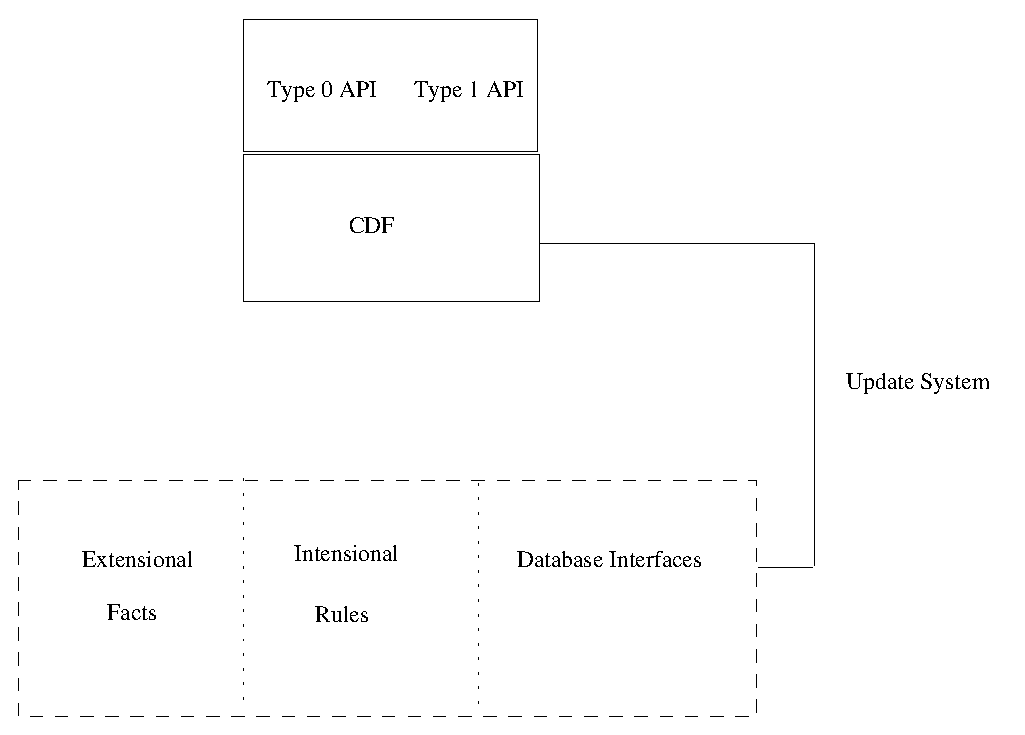
\epsfig{file=Figures/arch.eps,width=0.80\textwidth}}
\caption{A High-Level Architecture of CDF and XJ}
\label{fig:arch}
\end{figure}
%--------------

CDF instances can be classified either as Type-0 or a Type-1, each of
which has its own interface.  Type-0 instances are useful for storing
large amounts of information; and consistency and implication in
Type-0 instances is computable in polynomial time.  Type-0 instances
describe classes by existential and universal relations, qualified
number restrictions, and relational hierarchies, but descriptions omit
negation and disjunction. Type-0 instances also support a direct
product construction for objects and classes.  
\mycomment{
These product classes and objects can be useful for representing
certain types of non-binary relations, and are particularly useful for
incorporating knowledge represented as RDF facts \cite{}.  }
Information in Type-0 CDF instances is tightly coupled to XSB's
query mechanism, and CDF ensures that only the most specific answers
(according to a given inheritance hierarchy) are returned for any
Type-0 query.

Type-1 instances extend Type-0 instances to describe classes using
negation and disjunction, and thus permit descriptions that are
equivalent to an expressive description logic.  In fact, a Type-1 CDF
instance can be seen as a knowledge base in which various classes are
described via {\em class expressions}, which correspond to formulas in
description logics.  Reasoning in Type-1 instances is done via the CDF
theorem-prover.  Using the Type-1 API, users may ask whether a given
class or object is consistent, whether a given class expression is
consistent with a class or object; or whether a given class expression
is entailed by a given class or object.  The problems of determining
consistency or entailment of a Type-1 class expression have a high
degree of complexity.  To solve these problems the CDF theorem prover
uses several heuristics, but a determined (or unlucky) user can always
find class expressions that require a large amount of time to check.

Of course, ontology management systems require many features in
addition to reasoning and representation features \cite{MGPS03}.  We
mention some of these features.

\begin{itemize}
\item {\em A Semantic Checking System}.  CDF has various mechanisms for
ensuring consistency of objects and classes both at the Type-0 or
Type-1 level.  Various levels of consistency can be checked during
various operations on the CDF instance.
%
\item {\em A Component System}. Reusability of ontologies is supported
by the {\em component} structure of CDF.  An ontology component may be
maintained by separate users or organizations in different locations
and assembled in various ways by applications.
%
\item {\em A Concurrency System}. (Non open-source) Based on the
component structure, the {\em concurrency} mechanism for CDF allows
users to update their own CDF instances and to periodically update a
common store. Naturally, the various mechanisms in CDF for ensuring
consistency that are vital to ensuring coherency when users update
their systems concurrently.
%
\item {\em Database Interfaces}. (Non open-souce) CDF supports various
interfaces to databases so that CDF facts can be stored in a database
or mapped to database tables.
\end{itemize}

Based on these features, CDF can support user interfaces in a number
of ways.  One of the most convenient is to use a XSB/Java interface
such as InterProlog~\cite{Cale01} or JAXSB~(see
\texttt{http://xsb.sourceforge.net}) and then write a user interface in
Swing or some other Java Graphics library.  One of the easiest ways to
do this is to make use of the {\em XJ system} which allows Swing Gui
objects to be represented as Prolog terms (the XJ system is non
open-source) From a systems perspective, a graphical interface is then
written XJ library Swing widgets or specialized XJ-CDF Swing widgets.
CDF per-se has the following graphical packages and applications.
%
\begin{itemize}
%
\item {\em An XJ Caching System}. Adds and deletes to CDF are extended
with a notification mechanism so that Java Swing objects (created with
XJ, XSB's graphics system) reflect the state of CDF even when it
dynamically changes.
%
\item {\em A Visual Editor}. Finally,  CDF supports a graphical editor
that allows users both to visualize an ontology and to perform the
functions mentioned so far.
\end{itemize}
%
Extensional facts, intensional rules, updates, the Type-0 and Type-1
interfaces, consistency checking predicates and the full component
system are available as an open-source package for XSB.  Other
features, concurrency mechanisms, specialized database interfaces, XJ
support and the editor are not open-source.  The open-source code can
be obtained via \texttt{xsb.sourceforge.net}.  Inquiries about the full
Coherent Description System should be made to
\texttt{ode@xsb.com}.




\chapter{Getting Started with XSB} \label{quick_start}
%=====================================================

This section describes the steps needed to install XSB under UNIX and
under Windows.

\section{Installing XSB under UNIX}
%==================================
\label{installation_options}

If you are installing on a UNIX platform, the version of XSB that you
received may not include all the object code files so that an
installation will be necessary.  The easiest way to install XSB is to
use the following procedure.

\begin{enumerate}
\item	Decide in which directory in your file system you want to install
  XSB and copy or move XSB there.
\item Make sure that after you have obtained XSB by anonymous ftp (using
  the {\tt bin}ary option) or from the web, you have uncompressed it by
  following the instructions found in the file {\tt README}.
  
\item Note that after you uncompress and untar the XSB tar file, a
  subdirectory {\tt XSB} will be tacked on to the current directory. All
  XSB files will be located in that subdirectory.
  
  In the rest of this manual, let us use {\tt \$XSB\_DIR} to refer to this
  subdirectory.  Note the original directory structure of XSB must be
  maintained, namely, the directory {\tt \$XSB\_DIR} should contain all the
  subdirectories and files that came with the distribution. In particular,
  the following directories are required for XSB to work: \verb'emu',
  \verb'syslib', \verb'cmplib', \verb'lib', \verb'packages', \verb'build',
  and \verb'etc'.

\index{configuration}

\item Change directory to {\tt \$XSB\_DIR/build} and then run these commands:
  %%
  \begin{quote}
    \tt
    configure\\
    \tt
    makexsb
  \end{quote}
  %%
  %%$
  This is it!
  
  In addition, it is now possible to install XSB in a shared directory
  ({\it e.g.}, {\tt /usr/local}) for everyone to use.  In this situation,
  you should use the following sequence of commands:
  %%
  \begin{quote}
    \tt
    configure --prefix=\$SHARED\_XSB\\
    \tt
    makexsb\\
    \tt
    makexsb install
  \end{quote}
  %%$
  where {\tt \$SHARED\_XSB}  denotes the shared directory where XSB is
  installed.  In all cases, XSB can be run using the script
  %%$
  \begin{quote}
    \tt
    \$XSB\_DIR/bin/xsb
  \end{quote}
  However, if XSB is installed in a central location, the script for
  general use is:
  \begin{quote}
    \verb'<central-installation-directory>/<xsb-version>/bin/xsb'
  \end{quote}
\end{enumerate}
  %%

{\bf Important:} The XSB executable determines the location of the
libraries it needs based on the full path name by which it was invoked.
The ``smart script'' \verb|bin/xsb| also uses its full path name to
determine the location of the various scripts that it needs in order to
figure out the configuration of your machine.  Therefore, there are certain
limitations on how XSB can be invoked.

Here are some legal ways to invoke XSB:
%%
\begin{enumerate}
\item  invoking the smart script \verb|bin/xsb| or the XSB executable using
  their absolute or relative path name.
\item using an alias for \verb|bin/xsb| or the executable.
\item creating a new shell script that invokes either \verb|bin/xsb| or the
  XSB executable using their {\em full\/} path names. 
\end{enumerate}
%%

Here are some ways that are guaranteed to not work in some or all cases:
%%
\begin{enumerate}
\item  creating a hard link to either \verb|bin/xsb| or the executable and
  using {\it it\/} to invoke XSB. (Symbolic links should be ok.)
\item changing the relative position of either \verb|bin/xsb| or the
  XSB executable with respect to the rest of the XSB directory tree.
\end{enumerate}
%%

The configuration script allows many different options to be
specified.  A full listing can be obtained by typing {\tt
\$XSB\_DIR/build/configure --help}.
%%
\begin{description}
\item[Type of Machine.]  The configuration script automatically detects
  your machine and OS type, and builds XSB accordingly. Moreover, you can
  build XSB for different architectures while using the same tree and the
  same installation directory provided, of course, that these machines are
  sharing this directory, say using NFS or Samba. All you will have to do
  is to login to a different machine with a different architecture or OS
  type, and repeat the above sequence of comands.
  
  The configuration files for different architectures reside in different
  directories, and there is no danger of an architecture conflict.
  Moreover, you can keep using the same {\tt ./bin/xsb} script regardless
  of the architecture. It will detect your configuration and will use the
  right files for the right architecture! 

  If XSB is being built on a machine running Windows in which Cygwin
  is installed, Cygwin and Windows are treated as separate operating
  systems, as their APIs are completely different.  If no previous
  configuration has been made, the configure script will attempt to
  use {\tt gcc} and other Unix facilities, and therefore will compile
  the system under Cygwin.  If this behavior is not desired, the
  option {\tt --with-wind} (equivalently, {\tt --with-os=wind}) uses a
  Window compiler and API.  If a user wants to ensure the Cygwin
  compiler is used (say after a previous configuration for Windows),
  the option {\tt -without-wind} can be used.  See
  Section~\ref{quick:DOS} for more details.

\index{cc} \index{gcc} \index{acc}  
\item[Choice of the C Compiler and Other options] \label{cc} The {\tt
  configure} script will attempt to use {\tt gcc}, if it is available.
  Otherwise, it will revert to {\tt cc} or {\tt acc}.  Some versions
  of {\tt gcc} are broken for particular platforms, in which case you
  would have to give {\tt configure} an additional directive {\tt
    --with-cc} (or {\tt --with-acc}).  If you must use some special
  compiler, use {\tt --with-cc=your-own-compiler}.  You can also use
  the {\tt optimization-level} option to disable the default C
  compiler optimization level.  (or {\tt --disable-optimization} to
  disable all compiler optimizations).  {\tt --enable-debug}, and
  there are many other options.  Finally, the {\tt force64} option
  forces compilation to use 64 bit mode on 64-bit machines that
  default to 32 bit compilation.  Type {\tt configure --help} to see
  them all. Also see the file~\verb'$XSB_DIR/INSTALL' for more
  details.

\item[XSB and Site-specific Information] Using the option {\tt
  --prefix=PREFIX} installs architecture-independent files in the
  directory {\tt PREFIX}, e.g. {\tt /usr/local}, which can be useful
  if XSB is to be shared at a site.  Using the option {\tt
    --site-prefix=DIR} installs site-specific libraries in {\tt
    DIR/site}.  Other options indicate directories in which to search
  for site-specific static and dynamic libraries, and for include
  files.

\item[Multi-threading] \version{} of XSB is the first version that
  supports multi-threading.  The multi-threaded engine is slightly
  slower than the single-threaded engine, mostly due to its need for
  concurrency control.  To obtain the benefits of multiple threads on
  a platform that supports either Posix or Windows threads (i.e.
  nearly all platforms) users must configure XSB with the directive
  {\tt enable-mt}.  The multi-threaded engine works with other
  configuration options, multi-threading can be compiled with batched
  or local scheduling, with the ODBC or Interprolog interfaces, and so
  on.

%%$
\index{InterProlog Interface}
\index{Oracle Interface}
\index{SModels Interface}
\index{XASP}
\index{ODBC Interface}
\index{Tck/Tk}

\item[Interfaces] Certain interfaces must be designated at
configuration time, including those to Oracle, ODBC, Smodels, Tck/Tk,
and Libwww.  However, the XSB-calling-C interface interface does not
need to be specified at configuration time.  If you wish to use the
InterProlog Java interface that is based on {\tt jni}, you must
specify this at configuration time; otherwise if you wish to use the
sockets-based Interprolog interface, it does not need to be specified
at configuration time.  See Volume 2 and the InterProlog site {\tt
www.declarativa.com} for details of specific interfaces

While the XSB configuration mechanism can detect most include and
library paths, use of certain interfaces may require information about
particular directories.  In particular the {\tt
--site-static-libraries} option might be needed if compiling with
support for statically linked packages (such as Oracle) or if your
standard C libraries are in odd places. Alternately, dynamic libraries
on odd places may need to be speficied at configuation time using the
{\tt --site-dynamic-libraries} option.  and finally, the {\tt
--site-includes} option might be needed if your standard header files
(or your {\tt jni.h} file) are in odd places, or if XSB is compiled
with ODBC support.  Type {\tt configure --help} for more details.

%%$
\index{scheduling strategy}
\item[Type of Scheduling Strategy.]  The ordering of operations within
a tabled evaluation can drastically affect its performance.  XSB
provides two scheduling strategies: Batched Evaluation and Local
Evaluation.  Local Evaluation ensures that, whenever possible,
subgoals are fully evaluated before there answers are returned, and
provides superior behavior for programs in which tabled negation is
used.  Batched Evaluation evaluates queries to reduce the time to the
first answer of a query.  Both evaluation methods can be useful for
different programs.  Since Version 2.4, Local Evaluation has been the
default evaluation method for XSB.  Batched Evaluation can be chosen
via the {\tt --enable-batched-scheduling} configure option.  Detailed
explanations of the scheduling strategies can be found in
\cite{JFLP-Scheduling}, and further experimentation in \cite{CaSW02}.

%
\end{description}

Other options are of interest to advanced users who wish to experiment
with XSB, or to use XSB for large-scale projects.  In general, however
users need not concern themselves with these options.

\subsection{Possible Installation Problems}


\paragraph*{Lack of Space for Optimized Compilation of C Code}
When making the optimized version of the emulator, the temporary space
available to the C compiler for intermediate files is sometimes not
sufficient. For example on one of our SPARCstations that had very
little {\tt /tmp} space the {\tt "-O4"} option could not be used for
the compilation of files {\tt emuloop.c}, and {\tt tries.c}, without
changing the default {\tt tmp} directory and increasing the swap
space.  Depending on your C compiler, the amount and nature of {\tt
/tmp} and swap space of your machine you may or may not encounter
problems.  If you are using the SUN C compiler, and have disk space in
one of your directories, say {\tt dir}, add the following option to
the entries of any files that cannot be compiled:

\demo{       -temp=dir}

\noindent
If you are using the GNU C compiler, consult its manual pages
to find out how you can change the default {\tt tmp} directory or how you
can use pipes to avoid the use of temporary space during compiling.
Usually changing the default directory can be done by declaring/modifying
the {\tt TMPDIR} environment variable as follows:

\demo{       setenv TMPDIR dir}

\paragraph*{Missing XSB Object Files}
When an object (*.xwam) file is missing from the {\tt lib} directories
you can normally run the {\tt make} command in that directory to
restore it (instructions for doing so are given in Chapter
\ref{quick_start}).  However, to restore an object file in the
directories {\tt syslib} and {\tt cmplib}, one needs to have a
separate Prolog compiler accessible (such as a separate copy of
XSB), because the XSB compiler uses most of the files in these
two directories and hence will not function when some of them are
missing.  For this reason, distributed versions normally include all
the object files in {\tt syslib} and {\tt cmplib}.

\section{Installing XSB under Windows}
\subsection{Using Cygnus Software's \mbox{CygWin32}}
\label{quick:cygwin}

This is easy: just follow the Unix instructions. This is the preferred way to
run XSB under Windows, because this ensures that all features of XSB are
available.


\subsection{Using Microsoft Visual C++}
\label{quick:DOS}
%==========================================

\begin{enumerate}
\item 
   XSB will unpack into a subdirectory named {\tt xsb}.
   Assuming that you have {\tt XSB.ZIP} in the {\tt \$XSB\_DIR} directory,
   you can issue the command
\begin{verbatim}
   unzip386 xsb.zip
\end{verbatim}
   which will install XSB in the subdirectory {\tt xsb}.

 \item If you decide to move XSB to some other place, make sure that the
   entire directory tree is moved --- XSB executable looks for the files it
   needs relatively to its current position in the file system.

\end{enumerate}


You can compile XSB under Microsoft Visual C++ compiler 
to create a console-supported top loop or a DLL by following
these steps:

\begin{enumerate}

\item
   cd build

\item
  Type:\\
  {\tt makexsb\_wind "CFG=option" ["DLL=yes"] ["ORACLE=yes"] ["SITE\_LIBS=libraries"]}
  %%
  \begin{itemize}
  \item The items in square brackets are optional.
  \item The options for {\tt CFG} are: \emph{release} or \emph{debug}.  The
    latter is used when you want to compile XSB with debugging enabled.
  \item The other parameters to {\tt makexsb\_wind} are optional. The {\tt DLL}
    parameter tells Visual C++ to compile XSB as a DLL. The {\tt ORACLE}
    parameter compiles XSB with support for Oracle DBMS. If {\tt ORACLE} is
    specified, you {\bf must} also specify the necessary Oracle libraries
    using the parameter {\tt SITE\_LIBS}.
  \end{itemize}
  %%
   
 \item The above command will compile XSB as requested and will put the XSB 
   executable in:
%%
\[
 \tt
 \$XSB\_DIR\backslash config\backslash \mbox{\tt x86-pc-windows}\backslash bin
 \backslash xsb.exe
\]
%%
   If you requested to compile XSB as a DLL, then the DLL will be placed in
%%
\[
 \tt
 \$XSB\_DIR\backslash config\backslash \mbox{\tt x86-pc-windows}\backslash
 bin \backslash xsb.dll
\]
%%
\end{enumerate}
%%
{\bf Note}: the XSB executable and the DLL can coexist in the same source
tree structure. However, if you first compiled  XSB as an executable and
then want to compile it as a DLL (or vice versa), then you must run 
%%
\begin{verbatim}
 makexsb_wind  clean  
\end{verbatim}
%%
in between.


\section{Invoking XSB}
%=====================

Under Unix, XSB can be invoked by the command:
\begin{quote}
       \tt \$XSB\_DIR/bin/xsb
\end{quote}
%%$
if you have installed XSB in your private directory.
If XSB is instaled in a shared directory ({\it e.g.}, \$SHARED\_XSB
for the entire site (UNIX only), then you should use
\begin{quote}
       \tt \$SHARED\_XSB/bin/xsb
\end{quote}
%%
In both cases, you will find yourself in the top level interpreter.  
As mentioned above, this script automatically detects the system
configuration you are running on and will use the right files and
executables. (Of course, XSB should have been built for that architecture
earlier.)

Under Windows, you should invoke XSB by typing:
\[
 \tt
 \$XSB\_DIR\backslash config\backslash \mbox{\tt x86-pc-windows}\backslash bin
 \backslash xsb.exe
\]
%%


You may want to make an alias such as {\tt \smallourprolog} to the above
commands, for convenience, or you might want to put the directory where the
XSB command is found in the {\tt \$PATH} environment variable. However, you
should {\bf not} make hard links to this script or to the XSB executable.
If you invoke XSB via such a hard link, XSB will likely be confused and will
not find its libraries.  That said, you {\bf can} create other scripts and
call the above script from there.

Most of the ``standard'' Prolog predicates are supported by XSB, 
so those of you who consider yourselves champion entomologists, can try
to test them for bugs now.  Details are in Chapter~\ref{standard}.


\section{Compiling XSB programs}
%===============================

All source programs should be in files whose names have the 
suffix {\tt .P}.  One of the ways to compile a program from a file in 
the current directory and load it into memory, is to type the query:
\begin{verbatim}
     [my_file].
\end{verbatim}
where \verb'my_file' is the name of the file, or preferably, the name
of the module (obtained from the file name by deleting the suffix {\tt .P}).
To find more about the module system of XSB see Section~\ref{Modules}.

If you are eccentric (or you don't know how to use an editor) you can also 
compile and load predicates input directly from the terminal by using the
command:
\begin{verbatim}
     [user].
\end{verbatim}
A {\tt CTRL-d} or the atom \verb'end_of_file' followed by a period 
terminates the input stream.


\section{Sample XSB Programs}
%============================

If for some reason you don't feel like writing your own XSB programs, 
there are several sample XSB programs in the directory: 
{\tt \$XSB\_DIR/examples}.  All contain source code.

The entry predicates of all the programs in that directory are given
the names {\tt demo/0} (which prints out results) and {\tt go/0}
(which does not print results).\footnote{
  %%
  This convention does not apply to the subdirectories of the examples
  directory, which illustrate advanced features of XSB.
  %%
  }
%%
Hence, a sample session might look like
(the actual times shown below may vary and some extra information is given
using comments after the \% character):

{\footnotesize
 \begin{verbatim}
my_favourite_prompt> cd $XSB_DIR/examples
my_favourite_prompt> $XSB_DIR/bin/xsb
XSB Version 2.0 (Gouden Carolus) of June 27, 1999
[i586-pc-linux-gnu; mode: optimal; engine: slg-wam; scheduling: batched]
| ?- [queens].
[queens loaded]

yes
| ?- demo.

% ...... output from queens program .......

Time used: 0.4810 sec

yes
| ?- statistics.

memory (total)         1906488 bytes:       203452 in use,      1703036 free
  permanent space       202552 bytes
  glob/loc space        786432 bytes:          432 in use,       786000 free
    global                                     240 bytes
    local                                      192 bytes
  trail/cp space        786432 bytes:          468 in use,       785964 free
    trail                                      132 bytes
    choice point                               336 bytes
  SLG subgoal space          0 bytes:            0 in use,            0 free
  SLG unific. space      65536 bytes:            0 in use,        65536 free
  SLG completion         65536 bytes:            0 in use,        65536 free
  SLG trie space             0 bytes:            0 in use,            0 free
   (call+ret. trie           0 bytes,     trie hash tables            0 bytes)

      0 subgoals currently in tables
      0 subgoal check/insert attempts inserted     0 subgoals in the tables
      0 answer  check/insert attempts inserted     0 answers  in the tables

       Time: 0.610 sec. cputime,  18.048 sec. elapsetime

yes
| ?- halt.          % I had enough !!!

End XSB (cputime 1.19 secs, elapsetime 270.25 secs)
my_favourite_prompt>
 \end{verbatim}
}


\section{Exiting XSB}
%====================

If you want to exit XSB, issue the command \verb'halt.' or
simply type \verb'CTRL-d' at the XSB prompt. To exit XSB while it is
executing queries, strike \verb'CTRL-c' a number of times.


%%% Local Variables: 
%%% mode: latex
%%% TeX-master: "manual1"
%%% End: 

\chapter{System Description} \label{chap:system}
\label{system}

% TLS: changing object file extensions.
% TLS: discuss relative paths.

Throughout this chapter, we use \verb'$XSB_DIR' to refer to the
directory in which XSB was installed.

\section{Entering and Exiting XSB}
%=================================

After the system has been installed, the emulator's executable code appears 
in the file:
\begin{verbatim}
                     $XSB_DIR/bin/xsb
\end{verbatim}
If, after being built, XSB is later installed  at a central location,
\verb'$SHARED_XSB', the emulators executable code appears in
\begin{verbatim}
                     $SHARED_XSB/bin/xsb
\end{verbatim}
Either of these commands invokes XSB's top level interpreter which is
the most common way of using XSB.

\version{} of XSB can also directly execute object code files from the
command line interface.  Suppose you have a top-level routine {\tt go}
in a file {\tt foo.P} that you would like to run from the UNIX or
Windows command line.  As long as {\tt foo.P} contains a directive
{\tt :- go.}, and {\tt foo} has been compiled to an object file ({\tt
foo.xwam}), then
\begin{verbatim}
                       $XSB_DIR/bin/xsb -B foo.xwam
\end{verbatim}
will execute {\tt go}, loading the appropriate files as
needed~\footnote{In XSB, all extensions except '.pl' --- (default
'.P', '.H', '.xwam', '.D' (output by mode inferencing), and '.A'
(assembly dump) --- are defined in C and Prolog code using macros in
{\tt \$XSB\_DIR/emu/extensions\_xsb.h} and can be changed by a user if
desired.  Of course, such a step should not be taken lightly, as it
can cause severe compatability problems.}.
%
In fact the command
\verb'$XSB_DIR/bin/xsb' is equivalent to the command:
\begin{verbatim}
             $XSB_DIR/bin/xsb -B $XSB_DIR/syslib/loader.xwam
\end{verbatim}
%%$

There are several ways to exit XSB.  A user may issue the
command \verb'halt.' or \verb'end_of_file', or simply type
\verb'CTRL-d' at the XSB prompt.  To interrupt XSB
while it is executing a query, strike \verb'CTRL-c'.

\section{The System and its Directories}
%=======================================
When installed, The XSB system resides in a single directory that
contains several subdirectories.  For completeness, we review the
information in all subdirectories.  Normally, only the documentation
and files in the Prolog subdirectories, particularly {\tt examples},
{\tt lib}, and {\tt packages} will be of interest to users.
\begin{enumerate}
\item {\tt bin} contains scripts that call XSB executables
for various configurations.
%
\item {\tt build} contains XSB configuration scripts.  You may
already be familiar with the {\tt build} directory, which is used to
build XSB.
%
\item {\tt config} contains executables and other files specific to
particular configurations.
%
\item {\tt docs} contains the user manuals and other documentation,
including the technical documentation manual for developers.
%
\item {\tt emu} contains the C source code for the XSB emulator, for
I/O and for various interfaces.
%
\item {\tt etc} contains miscellaneous files used by XSB.
%
\item {\tt examples} contains some examples for Prolog, tabling,
HiLog and various interfaces.
%
\item {\tt cmplib} contains Prolog source and object code for the
compiler. 
%
\item {\tt gpp} contains a copy of the Gnu pre-processor used to
preprocess Prolog files.
%
\item {\tt lib} contains Prolog source and object code for extended
libraries. 
%
\item {\tt packages} The directory {\tt packages} contains the various
applications, such as FLORA, the XMC model checker and many others.
These applications are written in XSB and can be quite useful, but are
not part of the XSB system per se.
%
\item {\tt Prolog\_includes} contains include files for the Prolog
libraries, which are preprocessed using GPP.
%
\item {\tt syslib} contains Prolog source and object code for core XSB
libraries. 
\end{enumerate}

\noindent
All Prolog source programs are written in XSB, and all object (byte
code) files contain SLG-WAM instructions that can be executed by the
emulator.  These byte-coded instructions are machine-independent, so
usually no installation procedure is needed for the byte code files.

\section{File Names and XSB}  \label{sec:filenames}
%
\index{base file name}
\index{file designator}
Three files are associated with Prolog source code in
XSB~\footnote{Other types of files may be associated with foreign code
--- see Volume 2.}.
\begin{itemize}
\item A single {\it source} file, whose name is the {\em base file name} plus 
      the an extension suffix ``{\tt .P}'' or if a {\tt .P} file
      cannot be found , {\tt .pl}.   
\item An {\it object (byte-code)} file, whose name consists of the
base file name plus the suffix ``{\tt .xwam}''.
\item An optional {\it header} file, whose name is the base file name plus 
      the suffix ``{\tt .H}''.  When used, the header file normally
      contains file-level declarations and directives while the source
      file usually contains the actual definitions of the predicates
      defined in that module.
\end{itemize}
%
Most of the XSB system predicates, such as {\tt consult/\{1,2\}}, {\tt
compile/\{1,2\}} and others are somewhat flexible in how they allow
file designation.  A file may be designated by a {\em file designator}
which can be a base file name, a source file name; or the relative or
absolute paths to a base or source file name.  Unfortunately, the
exact semantics of a file designator differs among system predicates
in \version, as well as among platforms.

\section{The Module System of XSB} \label{Modules}
%========================================================
XSB has been designed as a module-oriented Prolog system.  Modules
provide a small step towards {\em logic programming ``in the large''}
that facilitates large programs or projects to be put together from
components which can be developed, compiled and tested separately.
Also module systems support the {\em principle of information hiding}
and can provide a basis for {\em data abstraction}.  The module system
of XSB is {\em file based} -- one module per file -- and {\em flat} --
modules cannot be nested.  In addition, XSB's module system is to some
extent {\em atom-based}, where any symbol in a module can be imported,
exported or be a local symbol, as opposed to the predicate-based ones
where this can be done only for predicate symbols~\footnote{Operator
  symbols can be exported as any other symbols, but their precedence
  must be redeclared in the importing module.}.

\index{module name}
By default, files are not treated as modules.  In order for a file to
be treated as a module, it must contain one or more {\it export
declarations}, which specify that a set of symbols appearing in that
module is visible and therefore can be used by any other module.  In
XSB, the {\em module name} is equal to the base file name in which the
module is defined.  Any file (either module or not) may also contain
{\it import declarations}, which allow symbols defined in and exported
by other modules to be used in the current module.  In addition, a
module can also contain {\it local declarations}, which specify that a
set of symbols are {\it visible by this module only}, and therefore
cannot be accessed by any other module.  Export, local, and import
declarations can appear anywhere in the source or header files and
have the following forms:

The module system of XSB is {\em file based} (one module per
file), {\em atom based} (where all non-predicate symbols are normally
assumed to be global to all modules), and {\em flat} (modules cannot

\demo{:- export $sym_1$, \ldots, $sym_l$. }

\demo{:- local $sym_1$, \ldots, $sym_m$. }

\demo{:- import $sym_1$, \ldots, $sym_n$ from $module$. }

\noindent
where $sym_i$ has the form $functor/arity$, and $module$ is a module
name.

We note that only exported symbols can be imported; for example
importing a local symbol will cause an {\tt environment conflict
error} when the file referred to by the import statement is loaded.
When a non-module file is loaded, its predicates and symbols are
loaded into the module {\tt usermod}, which is the working module of
the XSB interpreter.  Dynamically asserted code is also loaded into
{\tt usermod}.

For modules, the base file name is stored in its byte code file, which
means that if the byte code file is renamed, the base file name is not
altered, and hence may cause confusion to the user and/or the system.
However, byte code files generated for non-modules can be safely
renamed.

In order to understand the semantics of modules, the user should keep
in mind that in a module oriented system, the name of each symbol is
identified as if it were prefixed with its module name (equivalently
its base file name), hence two symbols of the same $functor/arity$ but
different module prefixes are distinct symbols.  Currently the
following set of rules is used to determine the module prefix of a
symbol:
\begin{itemize}
\item	Every predicate symbol appearing in a module (i.e. that appears as
	the head of some clause) is assumed by default to be {\em
	local} to that module unless it is declared otherwise (via an
	export or import declaration).  Symbols that are local to a
	given module are not visible to other modules.
\item	Every other symbol (essentially function symbols) in a module is
	assumed to be {\em global} (its module prefix is {\tt
	usermod}) unless declared otherwise.
\item	If a symbol is imported from another module (via an explicit import 
	declaration), the module prefix of the symbol is the module it
	is imported from; any other symbol takes the module where the
	symbol occurs as its module prefix.
\item	The XSB command-line interpreter treats {\tt usermod} as its
working module. 
\item	Symbols that are either defined in non-modules loaded into the
	system or that are dynamically created (by the use of standard
	predicates such as {\tt read/1, functor/3, '=..'/2}, etc) are
	contained in {\tt usermod}%
\footnote{The standard predicates of XSB are listed in {\tt
\$XSB\_DIR/syslib/std\_xsb.P}.}.  \index{standard predicates}
\end{itemize}
%
The following facts about the module system of XSB may not be
immediately obvious:
\begin{itemize}
\item   If users want to use a symbol from another module, they must
        explicitly import it otherwise the two symbols are different
        even if they are of the same $functor/arity$ form.
\item	A module can only export predicate symbols that are defined in
        that module.  As a consequence, a module {\em cannot} export
        predicate symbols that are imported from other modules.
        This happens because an {\tt import} declaration is just a
        request for permission to use a symbol from a module where
        its definition and an {\tt export} declaration appear.
\item   The implicit module for a particular symbol appearing in a
        module must be uniquely determined.  As a consequence, a
        symbol of a specific $functor/arity$ {\em cannot} be declared
        as both exported and local, or both exported and imported from
        another module, or declared to be imported from more than one
        module, etc.  These types of environment conflicts are
        detected at compile-time and abort the compilation.
\item   It is an error to import a symbol from a module that does not
        export it.  This error is {\em not\/} detected at compile-time
        but at run-time when a call to that symbol is made.  If the
        symbol is defined in, but not exported from the module that
	defines it, an environment conflict error will take place.
	If the symbol is not defined in that module an undefined
	predicate/function error will be be reported to the user.
	\index{errors!undefined predicate}
\item   In the current implementation, at any time only one symbol of
        a specific $functor/arity$ form can appear in a module.  As an
        immediate consequence of this fact, only one $functor/arity$
        symbol can be loaded into the current working module ({\tt
        usermod}).  An attempt to load a module that redefines that
        symbol results in a warning to the user and the newly loaded
        symbol {\em overrides} the definition of the previously loaded
        one.
\end{itemize}

\paragraph*{Usage inference and the module system}
The import and export statements of a module $M$ are used by the
compiler for inferring usage of predicates.  At compilation time, if a
predicate $P/N$ occurs as callable in the body of a clause defined in
$M$, but $P$ is neither defined in $M$ nor imported into $M$ from some
other module, a warning is issued that $P/N$ is undefined.  Here
``occurs as callable'' means that $P/N$ is found as a literal in the
body of a clause, or within a system meta-predicate, such as {\tt
assert/1}, {\tt findall/3}, etc.  Currently, occurrences of a term
inside user-defined meta-predicates are not considered as callable by
XSB's usage inference algorithm.  Alternatively, if $P/N$ is defined in
$M$, it is {\em used} if $P/N$ is exported by $M$, or if $P/N$ occurs
as callable in a clause for a predicate that is used in $M$.  The
compiler issues warnings about all unused predicates in a module.  On
the other hand, since all modules are compiled separately, the usage
inference algorithm has no way of checking whether a predicate
imported from a given module is actually exported by that module.

\index{xsbdoc}
\index{\texttt{document\_export/1}}
\index{\texttt{document\_import/1}}
Usage inference can be highly useful during code development for
ensuring that all predicates are defined within a set of files, for
eliminating dead code, etc.  In addition, import and export
declarations are used by the {\tt xsbdoc} documentation system to
generate manuals for code~\footnote{Further information on {\tt
xsbdoc} can be found in {\tt \$XSB\_DIR/packages/xsbdoc}.}.  For these
reasons, it is sometimes the case that usage inference is desired even
in situations where a given file is not ready to be made into a
module, or it is not appropriate for the file to be a module for some
other reason.  In such a case the directives {\tt document\_export/1}
and {\tt document\_import/1} can be used, and have the same syntax as 
{\tt export/1} and {\tt import/1}, respectively.  These directives
affect only usage inference and {\tt xsbdoc}.  A file is treated as a
module if and only if it includes an {\tt export/1} statement, and
only {\tt import/1} statements affect dynamic loading and name
resolution for predicates.

\section{Standard Predicates in XSB} \label{sec:standard}
%========================================================

Whenever XSB is invoked, a large set of {\em standard} predicates are
defined and can be called from the interpreter or other
interface~\footnote{Such predicates are sometimes called ``builtins''
in other Prologs.}.  These predicates include the various ISO
predicates~\cite{}, along with predicates for tabling, I/O and for
interaction with the operating system, for HiLog, and for other
functionality.  Standard predicates are declared in the file {\tt
\$XSB\_DIR/syslib/std\_xsb.P} and are covered in
Chapter~\ref{standard} of this manual.  If a user wishes to redefine a
standard predicate, she has several choices.  First, the appropriate
fact in {\tt \$XSB\_DIR/syslib/std\_xsb.P} should be commented out.
Once this is done, a user may define the predicate as any other user
predicate.  Alternately, the compiler option {\tt allow\_redefinition}
can be used to allow the compiler to redefine a standard predicate
(Section~\ref{sec:CompilerOptions}).  If a user wants to make a new
definition or new predicate standard, the safest course is to put the
predicate into a module in the {\tt lib} directory, and add or modify
an associated fact in {\tt \$XSB\_DIR/syslib/std\_xsb.P}.

%========================================================
\section{The Dynamic Loader and its Search Path} \label{LibPath}
\index{load search path}

XSB differs from some other Prolog system in its ability to {\tt
dynamically} load modules.  In XSB, the loading of user modules Prolog
libraries (such as the XSB compiler) is delayed until predicates in
them are actually needed, saving program space for large Prolog
applications.  Dynamic loading is done by default, unlike other
systems where it is not the default for non-system libraries.

When a predicate imported from another module (see
Section~\ref{Modules}) is called during execution, the dynamic loader
is invoked automatically if the module is not yet loaded into the
system, The default action of the dynamic loader is to search for the
byte code file of the module first in the system library directories
(in the order {\tt lib, syslib}, and then {\tt cmplib}), and finally
in the current working directory.  If the module is found in one of*sh
these directories, then it will be loaded ({\em on a first-found
basis}). Otherwise, an error message will be displayed on the current
error stream reporting that the module was not found.  Because system
modules are dynamically loaded, the time it takes to compile a file is
slightly longer the first time the compiler is invoked in a session
than for subsequent compilations.


\subsection{Changing the Default Search Path and the Packaging System}
%=========================================================

The default search path of the dynamic loader can easily be changed by
having a file named {\verb|.xsb/xsbrc.P|} in the user's home
directory.  User-supplied library directories are searched by the
dynamic loader {\em before} searching the default library directories.
\index{\texttt{library\_directory/1}}  The {\verb|.xsb/xsbrc.P|} file,
which is automatically consulted by the XSB interpreter, might look
like the following:
\begin{verbatim}
             :- assert(library_directory('./')).
             :- assert(library_directory('~/')).
             :- assert(library_directory('/usr/lib/sbprolog')).
\end{verbatim}
After loading the module of the above example, the current working
directory is searched first, then the user's home directory,, then
{\tt "/usr/lib/sbprolog/"}, and finally XSB's system library
directories ({\tt lib, syslib}, and {\tt cmplib}).  XSB also uses {\tt
library\_directory/1} for internal purposes.  For instance, before the
user's {\verb|.xsb/xsbrc.P|} is consulted, XSB puts the {\tt packages}
directory and the directory \verb|.xsb/config/$CONFIGURATION| on the
library search path.  The directory
\verb'.xsb/config/$CONFIGURATION' is used to store user libraries that
are machine or OS dependent. (\verb'$CONFIGURATION' for a machine is
something that looks like {\tt sparc-sun-solaris2.6} or {\tt
pc-linux-gnu}, and is selected by XSB automatically at run time).  

Note that the file {\verb|.xsb/xsbrc.P|} is not limited to setting the
library search path.  In fact, arbitrary Prolog code can go there.

We emphasize that in the presence of a {\verb|.xsb/xsbrc.P|} file {\em
it is the user's responsibility to avoid module name clashes with
modules in XSB's system library directories}.  Such name clashes can
cause unexpected behavior as system code may try to load a user's
predicates.  The list of module names in XSB's system library
directories can be found by looking through the directories {\tt
\$XSB\_DIR/\{syslib,cmplib,lib\}}.

\index{packages}
Apart from the user libraries, XSB now has a simple packaging system.
A {\em package\/} is an application consisting of one or more files that
are organized in a subdirectory of one of the XSB system or user libraries.
The system directory \verb|$XSB_DIR/packages| has several examples
%%$
of such packages, many of which are documented in Volume 2 of this
manual, or contain their own manuals.  Packages are convenient
as a means of organizing large XSB applications, and for simplifying
user interaction with such applications.  User-level packaging is
implemented through the predicate
%%
\begin{verbatim}
     bootstrap_userpackage(+LibraryDir, +PackageDir, +PackageName).
\end{verbatim}
%%
\index{\texttt{bootstrap\_userpackage/3}}
which must be imported from the {\tt packaging} module. 

To illustrate, suppose you wanted to create a package, {\tt foobar}, inside
your own library, {\tt my\_lib}. Here is a sequence of steps you can
follow:  
%%
\begin{enumerate}
\item Make sure that {\tt my\_lib}\ is on the library search path by putting
  an appropriate assert statement in your {\tt xsbrc.P}.
\item Make a subdirectory \verb|~/my_lib/foobar| and organize all the
  package files there. Designate one file, say, {\tt foo.P}, as the
  entry point, {\it i.e.}, the application file that must be loaded first.
\item Create the interface program \verb|~/my_lib/foobar.P| with the
  following content:
    %%
    \begin{verbatim}
           :- bootstrap_userpackage('~/my_lib', 'foobar', foobar), [foo].
    \end{verbatim}
    %%
  The interface program and the package directory do not need to have the
  same name, but it is convenient to follow the above naming schema.
\item Now, if you need to invoke the {\tt foobar} application, you can
  simply type \verb|[foobar].| at the XSB prompt. This is because both and
  \verb|~/my_lib/foobar| have already been automatically added to the
  library search path.
\item If your application files export many predicates, you can simplify
  the use of your package by having \verb|~/my_lib/foobar.P| import all
  these predicates, renaming them, and then exporting them. This provides a
  uniform interface to the {\tt foobar} module, since all the package
  predicates are can now be imported from just one module, {\tt foobar}.
\end{enumerate}
%%
In addition to adding the appropriate directory to the library search
path, the \verb|bootstrap_userpackage/3| predicate also adds
information to the predicate \verb|package_configuration/3|, so that
other applications could query the information about loaded packages.

Packages can also be unloaded using the predicate
\verb|unload_package/1|. For instance, 

%%
\begin{verbatim}
       :- unload_package(foobar).  
\end{verbatim}
%%
removes the directory \verb|~/my_lib/foobar| from the library search path
and deletes the associated information from \verb|package_configuration/3|.
\index{\texttt{unload\_package/1}}
\index{\texttt{package\_configuration/2}}

Finally, if you have developed and tested a package that you think is
generally useful and you would like to distribute it with XSB, please
contact {\tt xsb-development@sourceforge.net}.


\subsection{Dynamically loading predicates in the interpreter}
%=============================================================
Modules are usually loaded into an environment when they are consulted
(see Section~\ref{Consulting}).  Specific predicates from a module can
also be imported into the run-time environment through the standard
predicate {\tt import PredList from Module}\index{\texttt{import/1}}.
Here, {\tt PredList} can either be a Prolog list or a comma list.
(The {\tt import/1} can also be used as a directive in a source module
(see Section~\ref{Modules}). \index{standard predicates}

We provide a sample session for compiling, dynamically loading, and
querying a user-defined module named {\tt quick\_sort}.  For this
example we assume that {\tt quick\_sort.P} is a file in the current
working directory, and contains the definitions of the predicates {\tt
concat/3} and {\tt qsort/2}, both of which are exported.

{\footnotesize
\begin{verbatim}
             | ?- compile(quick_sort).
             [Compiling ./quick_sort]
             [quick_sort compiled, cpu time used: 1.439 seconds]

             yes
             | ?- import concat/3, qsort/2 from quick_sort. 

             yes
             | ?- concat([1,3], [2], L), qsort(L, S).

             L = [1,3,2]
             S = [1,2,3]

             yes.
\end{verbatim}
}

The standard predicate {\tt import/1} does not load the module 
containing the imported predicates, but simply informs the system 
where it can find the definition of the predicate when (and if) the
predicate is called.


\section{Command Line Arguments} \label{sec:EmuOptions}
%========================================================
\index{emulator!command line options}
\index{options!command line arguments}
\index{stacks!default sizes}
\index{stacks!expanding}
%========================================================

There are several command line options for the emulator. The general 
synopsis obtained by the command {\tt \$XSB\_DIR/bin/xsb --help} is: 
{\small 
\begin{verbatim}
xsb [flags] [-l] [-i]
xsb [flags] -n
xsb [flags] module
xsb [flags] -B boot_module [-D cmd_loop_driver] [-t] [-e goal]
xsb [flags] -B module_to_disassemble -d
xsb -[h | v]
xsb --help | --version | --nobanner | --quietload | --noprompt

memory management flags:
    -c tcpsize | -m glsize | -o complsize | -u pdlsize | -r | -g gc_type
miscellaneous flags:
    -s | -S | -T

module:
    Module to execute after XSB starts up.
    Module should have no suffixes, no directory part, and
    the file module.xwam must be on the library search path.
boot_module:
    This is a developer's option.
    The -B flags tells XSB which bootstrapping module to use instead
    of the standard loader.  The loader must be specified using its
    full pathname, and boot_module.xwam must exist.
module_to_disassemble:
    This is a developer's option.
    The -d flag tells XSB to act as a disassembler.
    The -B flag specifies the module to disassemble.
cmd_loop_driver:
    The top-level command loop driver to be used instead of the
    standard one.  Usually needed when XSB is run as a server.
 
             -i : bring up the XSB interpreter
        -e goal : evaluate goal when XSB starts up
             -l : the interpreter prints unbound variables using letters
             -n : used when calling XSB from C
             -B : specify the boot module to use in lieu of the standard loader
             -D : Sets top-level command loop driver to replace the default
             -t : trace execution at the SLG-WAM instruction level
                   (for this to work, build XSB with the --debug option)
             -d : disassemble the loader and exit
           -c N : allocate N KB for the trail/choice-point stack
           -m N : allocate N KB for the local/global stack
           -o N : allocate N KB for the SLG completion stack
           -u N : allocate N KB for the SLG unification stack
             -r : turn off automatic stack expansion
     -g gc_type : choose heap garbage collection ("none", "sliding", 
                                                  "indirection", or "copying") 
             -p : enable Prolog profiling thru use of profile_call/1
             -s : maintain detailed statistical information
             -S : set default tabling method to subsumption-based
             -T : print a trace of each called predicate
--max_threads N : maintain information for up to N threads
  -v, --version : print the version and configuration information about XSB
     -h, --help : print this help message
     --nobanner : don't show the XSB banner on startup
    --quietload : don't show the `module loaded' messages
     --noprompt : don't show prompt (for non-interactive use)

\end{verbatim}
}
The order in which these options appear makes no difference.

\begin{description}
\item[{\tt -i}] Brings up the XSB interpreter.  This is the normal use
        and because of this, use of this option is optional and is
        only kept for backwards compatibility.
\item[{\tt -e goal}] Pass {\tt goal}  to XSB at startup. This goal is evaluated
    right before the first prompt is issued. For instance, 
    \verb'xsb -e "write('Hello!'), nl."'
    will print a heart-warming message when XSB starts up.
\item[{\tt -l}] Forces the interpreter to print unbound variables as
	letters, as opposed to the default setting which prints
	variables as memory locations prefixed with an underscore.
	For example, starting XSB's interpreter with this option will
	print the following:
        \begin{verbatim}
                  | ?- Y = X, Z = 3, W = foo(X,Z).

                  Y = A
                  X = A
                  Z = 3
                  W = foo(A,3)
	\end{verbatim}
	as opposed to something like the following:
	\begin{verbatim}
                  | ?- Y = X, Z = 3, W = foo(X,Z).

                  Y = _10073976
                  X = _10073976
                  Z = 3
                  W = foo(_10073976,3);
	\end{verbatim}
\item[{\tt -n}] used in conjunction with the {\tt -i} option, to
    indicate that the usual read-eval-print top-loop is not to be
    entered, but instead will interface to a calling C program.  See
    the chapter {\it Calling XSB from C} in Volume 2  for details.
\item[{\tt -d}] Produces a disassembled dump of {\tt byte\_code\_file} to 
    {\tt stdout} and exits.
\item[{\tt -c} {\em size}] Allocates {\em initial  size\/} KBytes of space
    to the trail/choice-point stack area.  The trail stack grows
    upward from the bottom of the region, and the choice point stack
    grows downward from the top of the region.  Because this region is
    expanded automatically from Version 1.6.0 onward, this option
    is rarely needed.  Default initial size: 768 KBytes.
\item[{\tt -m} {\em size}] Allocates {\em size\/} KBytes
    of space to the local/global stack area.  The global stack grows 
    upward from the bottom of the region, and the local stack grows 
    downward from the top of the region.  Default: 768 KBytes.
\item[{\tt -o} {\em size}] Allocates {\em size\/} KBytes of space
    to the completion stack area.  Because this region is expanded
    automatically from Version 1.6.0 onward, this option is rarely
    needed. Default initial size 64 KBytes.
\item[{\tt -u} {\em size}] Allocates {\em size} KBytes of space
    to the unification (and table copy) stack.  Default 64 KBytes.
    (This option is rarely needed.)
\item[{\tt -D}] Tells XSB to use a top-level command loop driver specified
  here instead of the standard XSB interpreter. This is most useful when
  XSB is used as a server.
\item[{\tt -t}] Traces through code at SLG-WAM instruction level.
  This option is intended for developers and is not fully supported.
  It is also not available when the system is being used at the
  non-debug mode (see Section~\ref{debugging}).
\item[{\tt -r}] Turns off automatic stack expansion.
%
\index{garbage collection}
\item[{\tt -g gc\_type}] Chooses the heap garbage collection strategy
  that is employed; choice of the strategy is between {\tt "none"}
  (meaning perform no garbage collection), or garbage collection based
  on {\tt sliding} on {\tt copying}, or on {\tt indirection} (See
  \cite{CATmem@ISMM-98} for descriptions of the first two garbage
  collectors, and \cite{CaSC01} for a description of the third).
%
\item[{\tt -p}] Enables the engine to collect information that can be
  used for profiling.  See Volume 2 of this manual for details.
%
\item[{\tt -s}] Maintains information on the size of program stacks
  for the predicate {\tt statistics/0}.  This option may be expected
  to slow execution by around 10\%.  Default: off.  Note: this option
  is not available with the multi-threaded engine.
\item[{\tt -S}] Indicates that tabled predicates are to be evaluated
    using subsumption-based tabling as a default for tabled predicates
    whose tabling method is not specified by using {\tt
    use\_variant\_tabling/1} or {\tt use\_subsumptive\_tabling/1} (see
    Section \ref{sec:TablePred:Decl&Mod}).  If this option is not
    specified, variant-based tabling will be used as the default tabling
    method by XSB\@.
\item[{\tt -T}] Generates a trace at entry to each called predicate
    (both system and user-defined).  This option is available mainly
    for people who want to modify and/or extend XSB, and it is
    {\em not\/} the normal way to trace XSB programs.  For the
    latter, the standard predicates {\tt trace/0} or {\tt debug/0}
    should be used (see Chapter~\ref{debugging}).

    Note: This option is not available when the system is being used
    at the non-tracing mode (see Section~\ref{debugging}).
  \item[{\tt --maxthreads N}] Allows XSB to maintain information for
    up to {\tt N} threads.  This means that XSB can currently run {\tt
      N} threads that are active, or that are inactive, non-detached,
    and not yet joined.
  \item[{\tt --nobanner}] Start XSB without showing the startup banner.
    Useful in batch scripts and for interprocess communication (when XSB is
    launched as a subprocess).
  \item[{\tt --quietload}] Do not tell when a new module gets loaded. Again, is
    useful in non-interactive activities and for interprocess communication.
  \item[{\tt --noprompt}] Do not show the XSB prompt. This is useful only in batch
    mode and in interprocess communication when you do not want the prompt
    to clutter the picture.
\end{description}

\comment{
As an example, a program which uses more heap and local stack than the
default configuration of XSB might be run by invoking XSB with the command.
\begin{verbatim}
         xsb -m 2000
\end{verbatim}
}

\section{Memory Management}\label{memory_management}
\index{memory management}
\index{garbage collection}
%===================================================
All execution stacks are automatically expanded in \version{},
including the local stack/heap region, the trail/choice point region,
and the completion stack region.  For the main thread, each of these
regions begin with an initial value set by the user at the
command-line or with a default value -- see
Section~\ref{sec:EmuOptions}).  Execution stacks increase their size
until it is not possible to do so with available system memory.  At
that point XSB tries to find the maximal amount of space that will
still fit in system memory.  When a thread is created within an XSB
process, the size of the thread's execution stacks may be set by {\tt
  xsb\_thread\_create/3}, otherwise the default values indicated in
Section~\ref{sec:EmuOptions} are used.  In addtion, whenever a thread
exits, memory specific to that thread is reclaimed.

Heap garbage collection is automatically included in XSB
\cite{CaSC01,CATmem@ISMM-98}.  (To change the algorithm used for heap
garbage collection or to turn it off altogether, see the predicate
{\tt garbage\_collection/1} or Section~\ref{sec:EmuOptions} for
command-line options).  In \version{} the default behavior is indirect
garbage collection.  Starting with \version{}, heap garbage collection
may automatically invokes garbage collection of XSB's ``string''
table, which stores Prolog's atomic constants.  Expansion and garbage
collection of execution stacks can occur when multiple threads are
active; however string garbage collection will not be invoked if there
is more than one active XSB thread.

The program area (the area into which XSB byte-code is loaded) is also
dynamically expanded as needed.  For dynamic code (created using {\tt
  assert/1}, or the standard predicates {\tt load\_dyn/1} and {\tt
  load\_dync/1}) index size is also automatically reconfigured.  Space
reclaimed for dynamic code depends on several factors.  If there is
only one active thread, space is reclaimed for retracted clauses and
abolished predicates as long as (1) there are no choice points that
may backtrack into the retracted or abolished code, and (2) if the
dynamic predicate is tabled, all of its tables are completed.
Otherwise, the code is marked for later garbage collection by {\tt
  gc\_dynamic/0}.  If more than one thread is active, private
predicates behave as just described, however space reclamation for
shared predicates will be delayed until there is a single active
thread.

Space for tables is dynamically allocated as needed and reclaimed
through use of the predicates {\tt abolish\_all\_tables/0}, {\tt
  abolish\_table\_pred/1}, {\tt abolish\_table\_call/1} and other
predicates.  As with dynamic code, space for tables may be reclaimed
immediately or marked for later garbage collection depending on
whether choice points may backtrack into the abolished tables, on the
number of active threads, etc.  See
Section~\ref{sec:TablePred:Deleting} for details.

\section{Compiling, Consulting, and Loading} \label{Consulting}
%====================================================
Like other Prologs, XSB provides for both statically compiled code and
dynamically asserted code.  Unlike some Prologs, however, there is no
difference between compiled and consulted code.  Abstractly,
``Compiling'' in XSB means creation of a file containing SLG-WAM
byte-code; ``Consulting'' means loading such a byte-code file, (and
perhaps creating the file itsef, via compilation).  Compiled code may
be more optimized than asserted code, but certain types of indexing,
such as trie and star indexing are (currently) available only for
dynamically asserted predicates (see {\tt index/2}).

\index{\texttt{consult/[1,2]}}
The standard predicate {\tt consult/[1,2]} is the most convenient
method for entering static source code rules into XSB's
database~\footnote{In XSB, {\tt reconsult/[1,2]} is defined to have
the same actions as {\tt consult/\{1,2\}}.}.  {\tt consult/1} has the
form: 
%
\begin{center}
{\tt consult(+Files)}
\end{center}
%
in which {\tt Files} is either a file designator (see
Section~\ref{sec:filenames}) or a list of file designators.  {\tt
consult/1} compiles any files specified in {\tt Files} that have been
touched later than their byte-code files, and loads them into XSB.  In
addition the form
%
\begin{center}{\tt
	    [Files]. 
}\end{center}
%
Is an alternative syntax for {\tt consult(Files)}.

{\tt consult/2} has the form.
\begin{center}{\tt
	consult(+Files, +CompilerOptionList) }
\end{center} 
{\tt Files} is as in {\tt consult/1} and {\tt CompilerOptionList}
is a list of options that are to be passed to the compiler if it is
invoked (alternatively, these compiler options can be declared in the
files themselves, as in Section~\ref{the_compiler}.  {\tt consult/2}
is more general than {\tt consult/1}, and {\tt consult(Files)} is
defined as {\tt 	consult(FileName, [])}.

Consulting a file (module) conceptually consists of the following five
steps which are described in detail in the following paragraphs.
\begin{description}
\item[Name Resolution:] determine the file to be consulted, including
	directory and drive location and extension.
\item[Compilation:]  if the source file has changed later than the
	object file, compile the module using predicate {\tt
            compile/2} with the options specified.
\item[Loading:] load the object code of the file into memory. 
\item[Importing:] if the file is a module, import any the exported
	predicates of that module to {\tt usermod}.
\item[Query Execution:] execute any queries that the file may contain.
\end{description}

There are two steps to name resolution: determining the proper
directory prefix and determining the proper file extension.  When {\tt
FileName} is absolute (i.e. it contains a path from the file to the
root of the file system) determining the proper directory prefix is
straightforward.  If {\tt FileName} is relative, i.e. it conains a
{\tt '/'} in Unix or {\tt '/'} in Windows, {\tt FileName} is expanded
to a directory prefix in an OS-dependent way, resolving symbols like
{\tt '.'}, {\tt '..'} and {\tt '\~{}'} when applicable.  However, the
user may also enter a name without any directory prefix. In this case,
the directory prefix is a directory in the dynamic loader path (see
Section~\ref{LibPath}) where the source file exists.  Once the
directory prefix is determined, the file name is checked for an
extension.  If there is no extension the loader first checks for a
file in the directory with the {\tt .P} extension, (or {\tt .c} for
foreign modules) before searching for a file without the extension,
and finally for a file with a {\tt .pl} extension.  Note that since
directories in the dynamic loader path are searched in a predetermined
order (see Section~\ref{LibPath}), if the same file name appears in
more than one of these directories, the compiler will consult the
first one it encounters.

Compilation is performed if the update date of a source file ({\tt
*.P/.pl} or {\tt *.H}) is later than that of the the object file ({\tt
*.xwam}).
%%
%----------------------------------------------------------------------
\comment{
{\em and} if the source file is not larger than the default compile
size.  This default compile is set to be 5000 words (via a declaration
in {\tt cmplib/config.P}), but can be reset by the user.  If the
source file is larger than the default compile size, the file will be
loaded using {\tt load\_dyn/1}, and otherwise it will be compiled
({\tt load\_dyn/1} can also be called separately, see the Section {\it
Asserting Dynamic Code} for details).  While {\tt load\_dyn} gives
reasonably good execution times, compilation can always be done by
using {\tt compile/[1,2]} explicitly.  }
%----------------------------------------------------------------------
%%
Currently (\version), a foreign language module is compiled when at
least one of files {\tt *.c} or {\tt *.H} has been changed from the
time the corresponding object files have been created.

Once the file is compiled into byte-code, the byte-code for the file
is loaded into XSB's database.  After loading the file all exported
predicates of that module are imported into the current environment
(the current working module {\tt usermod}) if the file is a module.
For non-modules, all predicates are imported into the current working
module.  As the last part of loading, any queries --- that is, any
terms with principal functor {\tt '?-'/1}, or with the principal
functor {\tt ':-'/1} and that are not directives like the ones
described in Section~\ref{the_compiler} are executed in the order that
they are encountered.

Error conditions for {\tt consult(+File)} are as follows: 
\bi
\item 	{\tt File} is not instantiated
\bi
\item 	{\tt instantiation\_error}
\ei
%
\item 	{\tt File} is not an atom
\bi
\item 	{\tt type\_error(atom,File)}
\ei
%
\item {\tt File} has been loaded previously in the session {\em and}
  there is more than one active thread.  \bi
\item 	{\tt misc\_error}
\ei
\ei

\paragraph*{The multifile directive}
\index{\texttt{multifile/2}}
The default action upon loading a file or module is to delete all
previous byte-code for predicates defined in the file.  If this is not
the desired behavior, the user may add to the file a declaration
\begin{center}
{\tt :- multifile Predicate\_List .} \\
\end{center}
where {\tt Predicate\_List} is a list of predicates in {\em
functor/arity\/} form.  The effect of this declaration is to delete
{\em only\/} those clauses of {\tt predicate/arity} that were defined
in the file itself.  Issues to remember when using {\tt multifile} in
XSB \version{} are:
%
\begin{itemize}
\item If a predicate {\tt p/n} is to be defined in more than one file,
{\tt p/n} must be declared as multifile in each file in which it is
defined. 
%
\item The {\tt multifile} declaration should be trusted only for
static code.  Multifile declarations are not supported for code that
is dynamically loaded (via {\tt load\_dyn/\{1,2\}} or {\tt
load\_dync/\{1,2\}}).
%
\end{itemize}

Other predicates for loading files are {\tt ensure\_loaded/\{1,2\}}.  

\begin{description}
\ouritem{ensure\_loaded(+FileName)}\index{\texttt{ensure\_loaded/1}}
%
This predicate checks to see whether the object file for {\tt
FileName} is newer than the source code and header files for {\tt
FileName}, and compiles {\tt FileName} if not.  If {\tt FileName} is
loaded into memory, {\tt ensure\_loaded/1} does not reload it, unlike
{\tt consult/1} which will always reload
\end{description}
% 
{\tt ensure\_loaded/2} is documented in Section~\ref{sec:LoadDyn}.

\section{The Compiler} \label{the_compiler} \index{Compiler}
%========================================================

The XSB compiler translates XSB source files into
byte-code object files.  It is written entirely in Prolog.
Both the sources and the byte code\index{byte code!files!compiler}
for the compiler can be found in the XSB system directory
{\tt cmplib}\index{Compiler!\texttt{cmplib}}.
%
\index{GPP}
Prior to compiling, XSB filters the programs through \emph{GPP}, a 
preprocessor written by Denis Auroux (auroux@math.polytechnique.fr).
This preprocessor maintains high degree of compatibility with the C
preprocessor, but is more suitable for processing Prolog programs.
The preprocessor is invoked with the compiler option \verb|xpp_on|
as described below. The various features of GPP are described in
Appendix~\ref{gpp-man}.

XSB also allows the programmer to use preprocessors other than GPP.
However, the modules that come with XSB distribution require GPP.
This is explained below (see \verb|xpp_on| compiler option).

The following sections describe the various aspects of the compiler 
in more detail.


\subsection{Invoking the Compiler} \label{compiler_invoking}
\index{invoking the Compiler}\index{Compiler!invoking}
%=====================================================

The compiler is invoked directly at the interpreter level (or in a 
program) through the Prolog predicates {\tt compile/[1,2]}.  

\index{\texttt{compile/[1,2]}}
 {\tt compile/2} has the form: 
\begin{center}{\tt	
	compile(+Files, +OptionList)
}
\end{center}
in which {\tt Files} is either an absolute or relative filename or a
ground list of absolute or relative file names; and {\tt OptionList}
is a ground list of compiler options.  {\tt compile/2} compiles all
files specified, using the compiler options specified in {\tt
OptionList} (see Section~\ref{sec:CompilerOptions} below for the
precise details.)

\demo{$|$ ?- compile(Files).} 

\noindent
is just a notational shorthand for the query:

\demo{$|$ ?- compile(Files, []).}

The standard predicates {\tt consult/[1,2]} call {\tt compile/1} (if
necessary).  

The list of compiler options {\tt OptionList}, if specified, 
should be a proper Prolog list, i.e.\ a term of the form:
\begin{center}
	{\tt [ $option_1$, $option_2$, $\ldots$, $option_n$ ].}
\end{center}
where $option_i$ is one of the options described in
Section~\ref{sec:CompilerOptions}.

The source file name corresponding to a given module is obtained by 
concatenating a directory prefix and the extension {\tt .P} (or other
filenames, see Section~\ref{sec:filenames}) 
to the module name.  The directory prefix must be in the
dynamic loader path (see Section~\ref{LibPath}).
Note that these directories are searched in a predetermined
order (see Section~\ref{LibPath}), so if a module with the same name
appears in more than one of the directories searched, the compiler 
will compile the first one it encounters.  In such a case, the user can 
override the search order by providing an absolute path name.

If {\tt File} contains no extension, an attempt is made to compile the
file {\tt File.P} (or other extensions) before trying compiling the
file with name {\tt File}.

We recommend use of the extension {\tt .P} for Prolog source file to
avoid ambiguity.  Optionally, users can also provide a header file for
a module (denoted by the module name suffixed by {\tt .H}).  In such a
case, the XSB compiler will first read the header file (if it
exists), and then the source file.  Currently the compiler makes no
special treatment of header files.  They are simply included in the
beginning of the corresponding source files, and code can, in
principle, be placed in either.  
\comment{
In future versions of XSB the
header files may be used to check interfaces across modules, hence it
is a good programming practice to restrict header files to
declarations alone.
}
 
The result of the compilation (an SLG-WAM object code file) is stored
in a ($\langle$filename$\rangle$.xwam), but {\tt compile/[1,2]} does {\em
not\/} load the object file it creates.  (The standard predicates {\tt
consult/[1,2]} and {\tt reconsult/[1,2]} both recompile the source
file, if needed, and load the object file into the system.)  The
object file created is always written into the directory where the
source file resides (the user must therefore have write permission
in that directory).
 
If desired, when compiling a module (file), clauses and directives can be
transformed as they are read.  This is indeed the case for definite clause
grammar rules (see Chapter~\ref{DCGs}), but it can also be done for clauses
of any form by providing a definition for predicate {\tt term\_expansion/2}
(see Section~\ref{DCG_builtins}).

Predicates {\tt compile/[1,2]} can also be used to compile foreign
language modules.  In this case, the names of the source files should
have the extension {\tt .c} and a {\tt .P} file must {\em not\/}
exist.  A header file (with extension {\tt .H}) {\em must} be present
for a foreign language module (see the chapter {\it Foreign Language
Interface} in Volume 2).


\subsection{Compiler Options}\label{sec:CompilerOptions}
\index{Compiler!options}\index{options!Compiler}
%=================================================

Compiler options can be set in three ways: from a global list of
options ({\tt set\_global\_compiler\_options/1}), from the
compilation command ({\tt compile/2} and {\tt consult/2}), and
from a directive in the file to be compiled (see compiler directive
{\tt compiler\_options/1}).

\begin{description}
\ouritem{set\_global\_compiler\_options(+OptionsList)}
\index{\texttt{set\_global\_compiler\_options/1}} 
    {\tt OptionsList} is a list of compiler options (described below).
    Each can optionally be prefixed by \verb|+| or \verb|-|,
    indicating that the option is to be turned on, or off,
    respectively.  (No prefix turns the option on.)  This evaluable
    predicate sets the global compiler options in the way indicated.
    These options will be used in any subsequent compilation, unless
    they are 
    reset by another call to this predicate, overridden by options
    provided in the compile invocation, or overridden by options in
    the file to be compiled.
\end{description}

The following options are currently recognized by the compiler:
\begin{description}
\item[{\tt optimize}]\index{\texttt{optimize}}
	When specified, the compiler tries to optimize the object code.
	In \version, this option optimizes predicate calls, among other
	features, so execution may be considerably faster for recursive
	loops.  However,
	due to the nature of the optimizations, the user may not be able to
	trace all calls to predicates in the program.  
%%
	\comment{TLS: can no longer assert to static code
	Also the Prolog code
	should be {\em static}.  In other words, the user is {\em not} allowed
	to alter the entry point of these compiled predicates by asserting new
	clauses.  }
%%
	As expected, the compilation phase will also be slightly
	longer.  For these reasons, the use of the {\tt optimize} option may
	not be suitable for the development phase, but is
	recommended once the code has been debugged.


\item[{\tt xpp\_on}]\index{\texttt{xpp\_on}}\index{GPP}
  Filter the program through a preprocessor  before sending it to the XSB 
  compiler. By default (and for the XSB code itself), XSB uses GPP, a
  preprocessor developed by Denis Auroux (auroux@math.polytechnique.fr)
  that has high degree of compatibility with the C preprocessor, but is
  more suitable for Prolog syntax. In this case, the source code can
  include the usual C 
  preprocessor directives, such as \verb|#define|, \verb|#ifdef|, and
  \verb|#include|. This option can be specified both as a parameter to
  compile/2 and as part of the {\tt compiler\_options/1} directive inside
  the source file. See Appendix~\ref{gpp-man} for more details on GPP.

  When an \verb|#include "file"| statement is encountered,
  XSB directs GPP preprocessor to search for the files to include in the
  directories \verb|$XSB_DIR/emu| 
  %%$
  and \verb|$XSB_DIR/prolog_includes|.
  %%$
  \index{\texttt{xpp\_include\_dir}}
  %%
  However, additional directories can be added to this search path by
  asserting into the predicate \verb|xpp_include_dir/1|, {\bf which must
    be imported from module} {\tt parse}.
  
  Note that when compiling XSB programs, GPP searches the current directory
  and the directory of the parent file that contains the include-directive
  \emph{last}. If you want additional directories to be searched, then the
  following statements must be executed:
%%
\begin{verbatim}
    :- import xpp_include_dir/1 from parse.
    :- assert(xpp_include_dir('some-other-dir')).
\end{verbatim}
%%
  If you want Gpp to search directories in a different order,
  {\tt xpp\_options/1} can be used (see below).

   Note: if you assert something into this predicate then you must also {\tt
    retractall(xpp\_include\_dir(\_))} after that or else subsequent Prolog
  compilations might not work correctly.

  XSB predefines the constant {\tt XSB\_PROLOG}, which can be used for
  conditional compilation. For instance, you can write portable program
  to run under XSB and and other prologs that support C-style
  preprocessing and use conditional compilation to account for the
  differences: 
  %%
  \begin{samepage}
  \begin{verbatim}
#ifdef XSB_PROLOG
    XSB-specific stuff
#else
    other Prolog's stuff
#endif
    common stuff
  \end{verbatim}
  \end{samepage}
  %%

  \index{xpp\_program}
  %%
  However, as mentioned earlier, XSB lets the user filter programs (except
  the programs that belong to XSB distribution) through any preprocessor
  the user wants. To this end, one only needs to assert the appropriate
  command into the predicate \verb|xpp_program|, which should be imported
  from module {\tt parse}. The command should not include the file
  name---XSB appends the name of the file to be compiled to the command
  supplied by the user. For instance, executing
  %%
  \begin{verbatim}
   :- assert(xpp_program('/usr/bin/m4 -E -G')).
  \end{verbatim}
  %%
  before calling the compiler will have the effect that the next XSB
  program passed to the compiler will be first preprocessed by the M4 macro
  package. Note that the XSB compiler automatically clears out the
  {\tt xpp\_program} predicate, so there is no need to tidy up each time.
  But this also means that if you need to compile several programs with a
  non-standard preprocessor then you must specify that non-standard
  preprocessor each time the program is compiled.
  
\item[{\tt xpp\_options}] \index{\texttt{xpp\_options}} This dynamic predicate
  must be imported from module {\tt parse}.  If some atom is asserted into
  {\tt xpp\_options} then this atom is assumed to be the list of command
  line options to be used by the preprocessor (only the first asserted atom
  is ever considered). If this predicate is empty, then the default list of
  options is used (which is {\tt '-P -m -nostdinc -nocurinc'}, meaning: use
  Prolog mode and do not search the standard C directories and the
  directory of the parent file that contains the include-instruction).
  
  As mentioned earlier, when XSB invokes Gpp, it uses the option {\tt
    -nocurinc} so that Gpp will not search the directory of the parent file. 
  If a particular application requires that the parent file directory
  must be searched, then this can be accomplished by executing 
  {\tt assert(xpp\_options('-P -m -nostdinc'))}.
  
  Note: if you assert something into this predicate then you must also {\tt
    retractall(xpp\_options(\_))} after that or else subsequent Prolog
  compilations might not work correctly.
  
\item[{\tt xpp\_dump}] \index{\texttt{xpp\_dump}}
  %%
  This causes XSB to dump the output from the GPP preprocessor into a file.
  If the file being compiled is named {\tt file.P} then the dump file is
  named {\tt file.P\_gpp}. This option can be included in the list of
  options in the {\tt compiler\_options/1} directive, but usually it is
  used for debugging, as part of the {\tt compile/2} predicate. If {\tt
    xpp\_dump} is specified directly in the file using {\tt
    compiler\_options/1} directive, then it should \emph{not} follow the
  {\tt gpp\_on} option in the list (or else it will be ignored).

\item[{\tt quit\_on\_error}] \index{\texttt{quit\_on\_error}}
  This causes XSB to exit if compilation of a program end with an error.
  This option is useful when running XSB from a makefile, when it is
  necessary to stop the build process after an error has been detected. For
  instance, XSB uses this option during its own build process.


%-------------------------------
\index{tabling!compiler options}
%-------------------------------
\item[{\tt auto\_table}]\index{\texttt{auto\_table}} When specified as a
  compiler option, the effect is as described in
  Section~\ref{tabling_directives}.  Briefly, a static analysis is made to
  determine which predicates may loop under Prolog's SLD evaluation.  These
  predicates are compiled as tabled predicates, and SLG evaluation is used
  instead.
%qkostis
\item[{\tt suppl\_table}]\index{\texttt{suppl\_table}} The intention of this
  option is to direct the system to table for efficiency rather than
  termination.  When specified, the compiler uses tabling to ensure that no
  predicate will depend on more than three tables or EDB facts (as
  specified by the declaration {\tt edb} of
  Section~\ref{tabling_directives}).  The action of {\tt suppl\_table} is
  independent of that of {\tt auto\_table}, in that a predicate tabled by
  one will not necessarily be tabled by the other.  During compilation,
  {\tt suppl\_table} occurs after {\tt auto\_table}, and uses table
  declarations generated by it, if any.
%--------------------------------------
\index{specialization!compiler options}
%--------------------------------------
\item[{\tt spec\_repr}]\index{\texttt{spec\_repr}}
	When specified, the compiler performs specialization of partially
	instantiated calls by replacing their selected clauses with the
	representative of these clauses, i.e. it performs {\em folding\/}
	whenever possible.  We note in general, the code replacement
	operation is not always sound; i.e. there
	are cases when the original and the residual program are not
	computationally equivalent.  The compiler checks for sufficient (but
	not necessary) conditions that guarantee computational equivalence.
	If these conditions are not met, specialization is not performed
	for the violating calls.
\item[{\tt spec\_off}]\index{\texttt{spec\_off}}
	When specified, the compiler does not perform specialization of
	partially instantiated calls.
\item[{\tt unfold\_off}]\index{\texttt{unfold\_off}}
	When specified, singleton sets optimizations are not performed
	during specialization.  This option is necessary in \version\
	for the specialization of {\tt table} declarations that select
	only a single chain rule of the predicate.
%qtls ??
\item[{\tt spec\_dump}]\index{\texttt{spec\_dump}}
	Generates a {\tt module.spec} file, containing the result of
	specializing partially instantiated calls to predicates defined
	in the {\tt module} under compilation.  The result is in Prolog
	source code form.

%---------------------------------------------
\index{unification factoring!compiler options}
%---------------------------------------------
\item[{\tt ti\_dump}]\index{\texttt{ti\_dump}}
	Generates a {\tt module.ti} file containing the result of applying
	unification factoring to predicates defined in the {\tt module}
	under compilation.  The result is in Prolog source code form.
	See page~\pageref{transformational_indexing} for more information
	on unification factoring.
\item[{\tt ti\_long\_names}]\index{\texttt{ti\_long\_names}}
	Used in conjunction with {\tt ti\_dump}, generates names for
	predicates created by unification factoring that reflect the
	clause head factoring done by the transformation.
\comment{
\item[{\tt init\_var\_off}]\index{\texttt{init\_var\_off}}
	When specified, the compiler will give a warning (instead of an
	error) upon finding that a potentially uninitialized variable is
	being used.  {\em Potentially uninitialized variables\/} are
	variables that appear in only one branch of an {\sf or} or an
	{\sf if-then-else} goal in the body, and, furthermore, are used
	after that goal.
	In certain clauses, the variable may always be initialized after
	the {\sf or} or the {\sf if-then-else} goal, because the execution 
	cannot continue through the path of the branch that does not initialize
	the variable.  In these cases, the {\tt init\_var\_off} option can be
	useful, though the user is cautioned against careless use of this
	option.

	{\sc Warning:} The object-file generated by the compiler when this
		option is used may not execute correctly (or even cause
		XSB to core dump!) if the variable is indeed
		uninitialized when used.
}
%---------------------------------------------
\index{mode analysis!compiler options}
%---------------------------------------------
\item[{\tt modeinfer}]\index{\texttt{modeinfer}}
	This option is used to trigger mode analysis. For each module
	compiled,  the mode analyzer creates a  {\tt {\em module}.D} file
	that contains the mode information.

	{\sc Warning:}
	Occasionally, the analysis itself may take a long time. 
	As far as we have seen,
	the analysis times are longer than the rest of the compilation time
	only when the module contains recursive predicates of arity $\geq 10$.
	If the analysis takes an unusually long time
	(say, more than 4 times as long as the rest of the compilation)
	you may want to abort and restart compilation without {\tt modeinfer}.
	
\item[{\tt mi\_warn}]\index{\texttt{mi\_warn}}
	During mode analysis, the {\tt .D} files corresponding to the
	imported modules are read in. The option {\tt mi\_warn} is used
	to generate warning messages if these {\tt .D} files are 
	outdated --- {\em i.e.}, older
	than the last modification time of the source files.

\item[{\tt mi\_foreign}] This option is used {\em only\/} when mode analysis
	is performed on XSB system modules. This option is
	needed when analyzing {\tt standard} and {\tt machine} in
	{\tt syslib}.


\item[{\tt sysmod}] \index{standard predicates}
	Mainly used by developers when compiling system modules. If
	specified, standard predicates (see {\tt
	/\$XSB\_DIR/syslib/std\_xsb.P}) are automatically available
	for use only if they are primitive predicates (see the file
	{\tt \$XSB\_DIR/syslib/machine.P} for a current listing of
	primitive predicates.  When compiling in this mode,
	non-primitive standard predicates must be explicitly imported
	from the appropriate system module.  Also standard predicates 
	are permitted to be defined.
\item[{\tt allow\_redefinition}] \index{standard predicates}
	By default the compiler refuses to compile a file that
	contains clauses that would redefine a standard predicate
	(unless the {\tt sysmod} option is in effect.)  By specifying
	this option, the user can direct the compiler to quietly allow
	redefinition of standard predicates.

\item[{\tt verbo}] Compiles the files (modules) specified in ``verbose'' mode, 
	printing out information about the progress of the compilation of each 
	predicate.
\item[{\tt profile}] This option is usually used when modifying the
	XSB compiler.  When specified, the compiler prints out
	information about the time spent in each phase of the
	compilation process.

\item[{\tt asm\_dump, compile\_off}] Generates a textual representation of 
	the SLG-WAM assembly code and writes it into the file {\tt module.A}
	where {\tt module} is the name of the module (file) being compiled.  
	
	{\sc Warning:} This option was created for compiler debugging and is
		not intended for general use.  There might be cases where
		compiling a module with these options may cause generation
		of an incorrect {\tt .A} and {\tt .xwam} file.  In such cases,
		the user can see the SLG-WAM instructions that are
		generated for a module by compiling the module as usual and
		then using the {\tt -d module.xwam} command-line
		option of the 
		XSB emulator (see Section~\ref{sec:EmuOptions}).
\item[{\tt singleton\_warnings\_off}] Does not print out any warnings
	for singleton variables during compilation.  This option can
	be useful for compiling generated programs.
\item[{\tt index\_off}] When specified, the compiler does not generate indices
	for the predicates compiled.  
\end{description}


\subsection{Specialization}\label{specialization}
\index{Compiler!specialization}\index{specialization!Compiler}
%=============================================================

From Version 1.4.0 on, the XSB compiler automatically performs
specialization of partially instantiated calls.  Specialization can be
thought as a source-level program transformation of a program to a
residual program in which partially instantiated calls to predicates
in the original program are replaced with calls to specialized versions
of these predicates.  The expectation from this process is that the
calls in the residual program can be executed more efficiently that
their non-specialized counterparts.  This expectation is justified
mainly because of the following two basic properties of the
specialization algorithm:
\begin{description}
\item[Compile-time Clause Selection] The specialized calls of the
	residual program  directly select (at compile time) a subset
	containing only the clauses that the corresponding calls of the
	original program would otherwise have to examine during their
	execution (at run time).  By doing so, laying down unnecessary
	choice points is at least partly avoided, and so is the need to
	select clauses through some sort of indexing.
\item[Factoring of Common Subterms] Non-variable subterms of partially
	instantiated calls that are common with subterms in the heads
	of the selected clauses are factored out from these terms
	during the specialization process.  As a result, some head
	unification ({\tt get\_*} or {\tt unify\_*}) and some argument
	register ({\tt put\_*}) WAM instructions of the original
	program become unnecessary.  These instructions are eliminated
	from both the specialized calls as well as from the specialized
	versions of the predicates.
\end{description}
Though these properties are sufficient to get the idea behind
specialization, the actual specialization performed by the XSB
compiler can be better understood by the following example.  The
example shows the specialization of a predicate that checks if a list
of HiLog terms is ordered:
\begin{center}
\tt
\begin{tabular}{ccc}
\begin{tabular}{l}
ordered([]). \\
ordered([X]). \\
ordered([X,Y|Z]) :- \\
\ \ \ \ X @=< Y, ordered([Y|Z]). 
\end{tabular}
& $\longrightarrow$ &
\begin{tabular}{l}
ordered([]). \\
ordered([X]). \\
ordered([X,Y|Z]) :- \\
\ \ \ \ X @=< Y, \_\$ordered(Y, Z). \\
\\
:- index \_\$ordered/2-2. \\
\_\$ordered(X, []). \\
\_\$ordered(X, [Y|Z]) :- \\
\ \ \ \ X @=< Y, \_\$ordered(Y, Z).
\end{tabular}
\end{tabular}
\end{center}
The transformation (driven by the partially instantiated call
{\tt ordered([Y|Z])}) effectively allows predicate {\tt ordered/2}
to be completely deterministic (when used with a proper list as its
argument), and to not use any unnecessary heap-space for its
execution.  We note that appropriate {\tt :- index} directives are
automatically generated by the XSB compiler for all specialized
versions of predicates.

The default specialization of partially instantiated calls is without
any folding of the clauses that the calls select.  Using the {\tt
spec\_repr} compiler option (see Section~\ref{sec:CompilerOptions})
specialization with replacement of the selected clauses with the
representative of these clauses is performed.  Using this compiler
option, predicate {\tt ordered/2} above would be specialized as follows:
%%
\begin{center}
\begin{minipage}{4.1in}
\begin{verbatim}
ordered([]).
ordered([X|Y]) :- _$ordered(X, Y).

:- index _$ordered/2-2.
_$ordered(X, []).
_$ordered(X, [Y|Z]) :- X @=< Y, _$ordered(Y, Z).
\end{verbatim}
\end{minipage}
\end{center}
%%$
%%
We note that in the presense of cuts or side-effects, the code
replacement operation is not always sound, i.e.  there are cases when
the original and the residual program are not computationally equivalent
(with respect to the answer substitution semantics).  The compiler
checks for sufficient (but not necessary) conditions that guarantee
computational equivalence, and if these conditions are not met,
specialization is not performed for the violating calls.

The XSB compiler prints out messages whenever it specialises
calls to some predicate.  For example, while compiling a file
containing predicate {\tt ordered/1} above, the compiler would print
out the following message:
\begin{center}
{\tt	\% Specialising partially instantiated calls to ordered/1}
\end{center}
The user may examine the result of the specialization transformation
by using the {\tt spec\_dump} compiler option
(see Section~\ref{sec:CompilerOptions}).

Finally, we have to mention that for technical reasons beyond the scope of
this document, specialization cannot be transparent to the user; predicates
created by the transformation do appear during tracing.


\subsection{Compiler Directives}\label{compiler_directives}
\index{Compiler!directives}\index{directives!Compiler}
%=====================================================

Consider a directive
\begin{verbatim}
:- foo(a).
\end{verbatim}
That occurs in a file that is to be compiled.  There are two logical
interpretations of such a directive.
\begin{enumerate}
\item {\tt foo(a)} is to be executed upon loading the file; or
%
\item{\tt foo(a)} provides information used by the compiler in
compiling the file. 
\end{enumerate}

By default, the interpretation of a directive is as in case (1) {\em
except} in the case of the compiler directives listed in this section,
which as their name implies, are taken to provide information to the
compiler.  Some of the directives, such as the {\tt mode/1} directive,
have no meaning as an executable directive, while others, such as {\tt
import/2} do.  In fact as an executable directive {\tt import/2}
imports predicates into {\tt usermod}.  For such a directive, a 
statement beginning with {\tt ?-}, such as 
\begin{verbatim}
?- import foo/1 from myfile.
\end{verbatim}
indicates that the directive should be executed upon loading the file,
and should have no meaning to the compiler.  On the other hand, the
statement
\begin{verbatim}
:- import foo/1 from myfile.
\end{verbatim}
Indicates that {\tt foo/1} terms in the file to be compiled are to be
understood as {\tt myfile:foo/1}.  In other words, the statement is
used by the compiler and will not be executed upon loading.  For
non-compiler directives the use of {\tt ?-} and {\tt :-} has no effect
--- in both cases the directive is executed upon loading the file.

The following compiler directives are recognized in \version\ of XSB
\footnote{Any parallelisation directives ({\tt parallel}) are simply
ignored by the compiler, but do not result in syntax errors to enhance
compatibility with various other earlier versions of PSB-Prolog.}.

\subsubsection{Mode Declarations}\label{mode_declarations}
\index{modes!directives}\index{directives!modes}
%-----------------------------------------------------

The XSB compiler accepts {\tt mode} declarations of the form:

\demo{:- mode $ModeAnnot_1, \ldots, ModeAnnot_n$.}

\noindent
where each $ModeAnnot$ is a {\em mode annotation\/} (a {\em term
indicator\/} whose arguments are elements of the set {\tt
$\{$+,-,\#,?$\}$}).  From Version 1.4.1 on, {\tt mode} directives are
used by the compiler for tabling directives, a use which differs from
the standard use of modes in Prolog systems\footnote{The most common
uses of {\tt mode} declarations in Prolog systems are to reduce the
size of compiled code, or to speed up a predicate's execution.}.  See
Section~\ref{tabling_directives} for detailed examples.

Mode annotations have the following meaning:
\begin{description}
\item[{\tt +}]
	This argument is an input to the predicate.  In every invocation
	of the predicate, the argument position must contain a non-variable
	term.  This term may not necessarily be ground, but the 
	predicate is guaranteed not to alter this argument).

	\demo{:- mode see(+), assert(+).}
\item[{\tt -}]
	This argument is an output of the predicate.  In every
	invocation of the predicate the argument
	position {\em will always be a variable\/} (as opposed to 
	the {\tt \#} annotation below).
	This variable is unified with the value returned by the predicate.
	We note that Prolog does not enforce the requirement that output
	arguments should be variables; however, output unification is not
	very common in practice.

	\demo{:- mode cputime(-).}
\item[{\tt \#}]
	This argument is either:
	\begin{itemize}
	\item	An output argument of the predicate for which a non-variable
		value may be supplied for this argument position.  If such a
		value is supplied, the result in this position is unified with
		the supplied supplied value.  The predicate fails if this
		unification fails.  If a variable term is supplied, the
		predicate succeeds, and the output variable is unified with
		the return value.

		\demo{:- mode '='(\#,\#).}
	\item	An input/output argument position of a predicate that has
		only side-effects (usually by further instantiating that
		argument).  The {\tt \#} symbol is used to denote the $\pm$
		symbol that cannot be entered from the keyboard.
	\end{itemize}
\item[{\tt ?}]
	This argument does not fall into any of the above categories. 
        Typical cases would be the following:
	\begin{itemize}
	\item	An argument that can be used both as input and as output
		(but usually not with both uses at the same time).

		\demo{:- mode functor(?,?,?).}
	\item	An input argument where the term supplied can be a variable
		(so that the argument cannot be annotated as {\tt +}), or is
		instantiated to a term which itself contains uninstantiated
		variables, but the predicate is guaranteed {\em not\/} to
		bind any of these variables.

		\demo{:- mode var(?), write(?).}
	\end{itemize}
\end{description}
We try to follow these mode annotation conventions throughout this manual.

Finally, we warn the user that {\tt mode} declarations can be error-prone,
and since errors in mode declarations do not show up while running the
predicates interactively, unexpected behavior may be witnessed in compiled
code, optimized to take modes into account (currently not performed by
XSB)\@.  However, despite this danger, {\tt mode} annotations can be
a good source of documentation, since they express the programmer's
intention of data flow in the program.


\subsubsection{Tabling Directives}\label{tabling_directives}
\index{tabling!directives}\index{directives!tabling}
%-----------------------------------------------------
\index{\texttt{auto\_table}}
Memoization is often necessary to ensure that programs terminate, and
can be useful as an optimization strategy as well.  The underlying
engine of XSB is based on SLG, a memoization strategy, which,
in our version, maintains a table of calls and their answers for each
predicate declared as {\em tabled}.  Predicates that are not declared
as tabled execute as in Prolog, eliminating the expense of tabling
when it is unnecessary.

The simplest way to use tabling is to include the directive

\demo{:- auto\_table.}

\noindent
anywhere in the source file.  {\tt auto\_table} declares predicates
tabled so that the program will terminate.

To understand precisely how {\tt auto\_table} does this, it is
necessary to mention a few properties of SLG.  For programs which have
no function symbols, or where function symbols always have a limited
depth, SLG resolution ensures that any query will terminate after it
has found all correct answers.  In the rest of this section, we
restrict consideration to such programs.

Obviously, not all predicates will need to be tabled for a program to
terminate.  The {\tt auto\_table} compiler directive tables only those
predicates of a module which appear to static analysis to contain an
infinite loop, or which are called directly through {\tt tnot/1}.  It
is perhaps more illuminating to demonstrate these conditions through
an example rather than explaining them.  For instance, in the program.

%tls commented out minipage because latex was formatting badly,
\begin{center}
%\begin{minipage}{3in}
\begin{verbatim}
:- auto_table. 

p(a) :- s(f(a)). 

s(X) :- p(f(a)).

r(X) :- q(X,W),r(Y).

m(X) :- tnot(f(X)).

:- mode ap1(-,-,+).
ap1([H|T],L,[H|L1]) :- ap1(T,L,L1).

:- mode ap(+,+,-).
ap([],F,F).
ap([H|T],L,[H|L1]) :- ap(T,L,L1).

mem(H,[H|T]).
mem(H,[_|T]) :- mem(H,T).
\end{verbatim}
%\end{minipage}
\end{center}

\noindent
The compiler prints out the messages
\begin{verbatim}
% Compiling predicate s/1 as a tabled predicate
% Compiling predicate r/1 as a tabled predicate
% Compiling predicate m/1 as a tabled predicate
% Compiling predicate mem/2 as a tabled predicate
\end{verbatim}

Terminating conditions were detected for {\tt ap1/3} and {\tt ap/3}, but
not for any of the other predicates.

{\tt auto\_table} gives an approximation of tabled programs which we
hope will be useful for most programs.  The minimal set of tabled
predicates needed to insure termination for a given program is
undecidable.  
\comment{
Practically, refining the set of tabled predicates
deduced by {\tt auto\_table} is still an open research problem.
}
It should be noted that the presence of meta-predicates such as {\tt
call/1} makes any static analysis useless, so that the {\tt
auto\_table} directive should not be used in such cases.

Predicates can be explicitly declared as tabled as well, through the
{\tt table/1}.  When {\tt table/1} is used, the directive takes the
form

\demo{:- table(F/A).}

\noindent
where {\tt F} is the functor of the predicate to be tabled, and {\tt A} its
arity.  

\index{\texttt{suppl\_table}}
Another use of tabling is to filter out redundant solutions for
efficiency rather than termination.  In this case, suppose that the
directive {\tt edb/1} were used to indicate that certain predicates were
likely to have a large number of clauses.  Then the action of the declaration
{\tt :- suppl\_table} in the program:
\begin{verbatim}
:- edb(r1/2).
:- edb(r2/2).
:- edb(r3/2).

:- suppl_table.

join(X,Z):- r1(X,X1),r2(X1,X2),r3(X2,Z).
\end{verbatim}
would be to table {\tt join/2}.  The {\tt suppl\_table} directive is
the XSB analogue to the deductive database optimization, {\em
supplementary magic templates} \cite{BeRa91}.  {\tt suppl\_table/0} is
shorthand for {\tt suppl\_table(2)} which tables all predicates
containing clauses with two or more {\tt edb} facts or tabled
predicates.  By specifying {\tt suppl\_table(3)} for instance, only
predicates containing clauses with three or more {\tt edb} facts or
tabled predicates would be tabled.  This flexibility can prove useful
for certain data-intensive applications.


\subsubsection{Indexing Directives}\label{indexing_directives}
\index{indexing!directives}\index{directives!indexing}
%-------------------------------------------------------------

The XSB compiler by default generates an index on the principal 
functor of the first argument of a predicate.  Indexing on the appropriate 
argument of a predicate may significantly speed up its execution time.  
In many cases the first argument of a predicate may not be the most
appropriate argument for indexing and changing the order of arguments
may seem unnatural.  In these cases, the user may generate an index
on any other argument by means of an indexing directive.  This is a
directive of the form:

\demo{:- index Functor/Arity-IndexArg.}

\noindent
indicating that an index should be created for predicate 
{\tt Functor}/{\tt Arity} on its ${\tt IndexArg}^{\rm th}$ argument.
One may also use the form:

\demo{:- index(Functor/Arity, IndexArg, HashTableSize).}

\index{\texttt{index/2}}
\noindent
which allows further specification of the size of the hash table to use for
indexing this predicate if it is a {\em dynamic} (i.e., asserted) predicate.
For predicates that are dynamically loaded, this directive can be used to
specify indexing on more than one argument, or indexing on a combination
of arguments (see its description on page~\pageref{index_dynamic}).
For a compiled predicate the size of the hash table is computed automatically,
so {\tt HashTableSize} is ignored.

All of the values {\tt Functor}, {\tt Arity}, {\tt IndexArg} (and possibly
{\tt HashTableSize}) should be ground in the directive.  More specifically,
{\tt Functor} should be an atom, {\tt Arity} an integer in the range 0..255,
and {\tt IndexArg} an integer between 0 and {\tt Arity}.  If {\tt IndexArg}
is equal to~0, then no index is created for that predicate. An {\tt index}
directive may be placed anywhere in the file containing the predicate it
refers to.

As an example, if we wished to create an index on the third argument 
of predicate {\tt foo/5}, the compiler directive would be:

\demo{:- index foo/5-3.}


\subsubsection{Unification Factoring}\label{transformational_indexing}
\index{indexing!transformational}
When the clause heads of a predicate have portions of arguments common
to several clauses, indexing on the principal functor of one argument
may not be sufficient.  Indexing may be improved in such cases by the
use of unification factoring.  Unification Factoring is a program
transformation that ``factors out'' common parts of clause heads,
allowing differing parts to be used for indexing, as illustrated by
the following example:
\begin{center}
\tt
\begin{tabular}{ccc}
\begin{tabular}{l}
p(f(a),X) :- q(X). \\
p(f(b),X) :- r(X).
\end{tabular}
& $\longrightarrow$ &
\begin{tabular}{l}
p(f(X),Y) :- \_\$p(X,Y). \\
\_\$p(a,X) :- q(X). \\
\_\$p(b,X) :- r(X).
\end{tabular}
\end{tabular}
\end{center}
The transformation thus effectively allows $p/2$ to be indexed
on atoms $a/0$ and $b/0$.  Unification Factoring is transparent
to the user; predicates created by the transformation are internal
to the system and do not appear during tracing.

The following compiler directives control the use of unification
factoring:\footnote{Unification factoring was once called
transformational indexing, hence the abbreviation {\tt ti} in the
compiler directives}.
\begin{description}
\item[{\tt :- ti(F/A).}] Specifies that predicate $F/A$ should be
	compiled with unification factoring enabled.
\item[{\tt :- ti\_off(F/A).}] Specifies that predicate $F/A$ should be
	compiled with unification factoring disabled.
\item[{\tt :- ti\_all.}] Specifies that all predicates defined in the
	file should be compiled with unification factoring enabled.
\item[{\tt :- ti\_off\_all.}] Specifies that all predicates defined in
	the file should be compiled with unification factoring disabled.
\end{description}
By default, higher-order predicates (more precisely, predicates named
{\it apply\/} with arity greater than 1) are compiled with unification
factoring enabled.  It can be disabled using the {\tt ti\_off}
directive.  For all other predicates, unification factoring must be
enabled explicitly via the {\tt ti} or {\tt ti\_all} directive.  If
both {\tt :- ti(F/A).} ({\tt :- ti\_all.}) and {\tt :- ti\_off(F/A).}
({\tt :- ti\_off\_all.}) are specified, {\tt :- ti\_off(F/A).} ({\tt
:- ti\_off\_all.}) takes precedence.  Note that unification factoring
may have no effect when a predicate is well indexed to begin
with.  For example, unification factoring has no effect on the
following program:
\begin{center}
\tt
\begin{tabular}{l}
p(a,c,X) :- q(X). \\
p(b,c,X) :- r(X).
\end{tabular}
\end{center}
even though the two clauses have $c/0$ in common.  The user may
examine the results of the transformation by using the {\tt ti\_dump}
compiler option (see Section~\ref{sec:CompilerOptions}).

\subsubsection{Other Directives} \label{other-directives}
%==============================================

XSB has other directives not found in other Prolog systems.

\begin{description}
\desc{:- hilog $atom_1, \ldots, atom_n$.}
	Declares symbols $atom_1$ through $atom_n$ as HiLog symbols.
	The {\tt hilog} declaration should appear {\em before} any use of
	the symbols.  See Chapter~\ref{Syntax} for a purpose of this
 	declaration.
\desc{:- ldoption($Options$).}
        This directive is only recognized in the header file ({\tt .H} file) 
	of a foreign module. See the chapter {\it Foreign Language
Interface} in Volume 2 for its explanation.
\desc{:- compiler\_options($OptionsList$).}
	Indicates that the compiler options in the list $OptionsList$
	should be used to compile this file.  This must appear at the
	beginning of the file.  These options will override any others,
	including those given in the compilation command.  The options
	may be optionally prefixed with \verb|+| or \verb|-| to
	indicate that they should be set on or off.  (No prefix
	indicates the option should be set on.)

\end{description}

\subsection{Inline Predicates}\label{inline_predicates}
\index{Compiler!inlines}\index{inlines!Compiler}
%======================================================

{\em Inline predicates} represent ``primitive'' operations in the WAM.
Calls to inline predicates are compiled into a sequence of WAM
instructions in-line, i.e. without actually making a call to the
predicate.  Thus, for example, relational predicates (like {\tt >/2},
{\tt >=/2}, etc.) compile to, essentially, a subtraction followed by a
conditional branch.  As a resut, calls to inline predicates will not
be trapped by the debugger, and their evaluation will not be visible
during a trace of program execution.  Inline predicates are expanded
specially by the compiler and thus {\em cannot be redefined by the
user without changing the compiler}.  The user does not need to import
these predicates from anywhere.  There are available no matter what
options are specified during compiling.

Table~\ref{inlinepredicatetable} lists the inline predicates of
XSB \version.  Those predicates that start with \verb|_$|
are internal predicates that are also expanded in-line during
compilation.

\begin{table}[htbp]\centering{\tt
\begin{tabular}{lllll}
\verb|'='/2|    &\verb|'<'/2|	&\verb|'=<'/2|  &\verb|'>='/2| &\verb|'>'/2| \\
\verb|'=:='/2|  &\verb|'=\='/2|	&is/2           &\verb|'@<'/2| &\verb|'@=<'/2|\\
\verb|'@>'/2|	&\verb|'@>='/2|	&\verb|'=='/2|	&\verb|'\=='/2|&fail/0  \\
true/0		&var/1		&nonvar/1	&halt/0	       &'!'/0   \\
'\_\$cutto'/1	&'\_\$savecp'/1	&'\_\$builtin'/1
\end{tabular}}
\caption{The Inline Predicates of XSB}\label{inlinepredicatetable}
\end{table}

We warn the user to be cautious when defining predicates whose functor
starts with {\tt \_\$} since the names of these predicates may
interfere with some of XSB's internal predicates.  The situation may
be particularly severe for predicates like {\tt '\_\$builtin'/1} that
are treated specially by the XSB compiler.

\section{A Note on ISO Compatability} \label{sec:iso}

In \version, an effort has been made to ensure compatability with the
Prolog ISO standard.  In this section, we mention the differences with
the ISO standard.  XSB implements almost all ISO builtins, although
there are certain semantic differences between XSB's implementation
and that of the ISO standard in certain cases.

The main difference of XSB with the ISO standard is in terms of
parsing.  \version{} of XSB does not support full ISO syntax, nor does
it support multiple character sets.  Rectifying these limitations is a
priority for future releases.

A second difference involves XSB's implementation of ISO streams.  XSB
can create streams from several first class objects, including pipes,
atoms, and consoles in addition to files.  However by default, XSB
opens streams in binary mode, rather than text mode in opposition to
the ISO standard, which opens streams in text mode.  This makes no
difference in UNIX or LINUX, for which text and binary streams are
identical, but does make a difference in Windows, where text files are
processed more than binary files.

% TLS: how about floats?
% public/private

The final difference involves error handling in XSB.  XSB implements a
catch and throw mechanism that is similar to the ISO standard.  In
addition, XSB usually thows errors for ISO-predicates under the same
conditions as specified in the standard.  The only differences in
error handling are: (1) the type of error thrown may differ in XSB due
to an effort to minimize the amount of checking performed; and (2) ISO
may specify domain errors in some cases in which XSB throws type
errors.  The reasons for this have to do with XSB's nascent type
system, as described in Section~\ref{sec:types}.  The difference in
error terms should cause minimal portability problems, as it only
affects the type terms thrown at error, and these terms are
implementation-dependant as defined in the standard.




%%% Local Variables: 
%%% mode: latex
%%% TeX-master: "manual1"
%%% End: 

\chapter{Syntax} \label{Syntax}
%==============================

The syntax of XSB is taken from C-Prolog with extensions to support
HiLog~\cite{ChKW93}~\footnote{Sporadic attempts are made to make XSB
ISO-compliant, contact us if you have a problem with syntax.}, which
adds certain features of second-order syntax to Prolog.

\section{Terms} \label{TermSyntax}
%=================================
The data objects of the HiLog language are called {\em terms}.
A {\em HiLog term} can be constructed from any logical symbol or a term
followed by any finite number of arguments.  In any case, a {\em term}
is either a {\em constant}, a {\em variable}, or a {\em compound term}.

A {\em constant} is either a {\em number} (integer or floating-point) or an
{\em atom}.  Constants are definite elementary objects, and correspond to
proper nouns in natural language.


\subsection{Integers}
The printed form of an integer in HiLog consists of a sequence of digits
optionally preceded by a minus sign ({\tt '-'}).  These are normally 
interpreted as base $10$ integers.  It is also possible to enter integers
in other bases ($2$ through $36$); this can be done by preceding the digit
string by the base (in decimal) followed by an apostrophe ({\tt '}).  If a
base greater than $10$ is used, the characters {\tt A-Z} or {\tt a-z} are
used to stand for digits greater than $9$.

Using these rules, examples of valid integer representations in XSB are:
\begin{verbatim}
           1    -3456    95359    9'888    16'1FA4    -12'A0    20'
\end{verbatim}
representing respectively the following integers in decimal base:
\begin{verbatim}
           1    -3456    95359     728       8100      -120      0
\end{verbatim}

Note that the following:
\begin{verbatim}
                   +525     12'2CF4     37'12     20'-23
\end{verbatim}
are not valid integers of XSB.

A base of $0$ (zero) will return the ASCII code of the (single) character
after the apostrophe; for example,
\begin{verbatim}
                                 0'A = 65
\end{verbatim}


\subsection{Floating-point Numbers}
A HiLog floating-point number consists of a sequence of digits with an
embedded decimal point, optionally preceded by a minus sign ({\tt '-'}), and
optionally followed by an exponent consisting of uppercase or lowercase
{\tt 'E'} and a signed base $10$ integer.

Using these rules, examples of HiLog floating point numbers are:
\begin{verbatim}
              1.0    -34.56    817.3E12    -0.0314e26    2.0E-1
\end{verbatim}
Note that in any case there must be at least one digit before, and one digit
after, the decimal point.


\subsection{Atoms}
A HiLog atom is identified by its name, which is a sequence of up to 1000
characters (other than the null character).  Just like a Prolog atom, a HiLog
atom can be written in any of the following forms:
\begin{itemize}
\item Any sequence of alphanumeric characters (including {\tt '\_'}), starting
      with a lowercase letter.

\item Any sequence from the following set of characters (except of the
      sequence {\tt '/*'}, which begins a comment):
      \begin{verbatim}
                     + - * / \ ^ < > = ` ~ : . ? @ # &
      \end{verbatim}

\item Any sequence of characters delimited by single quotes, such as:
      \begin{verbatim}
                         'sofaki'    '%'    '_$op'
      \end{verbatim}
      If the single quote character is to be included in the sequence it must
      be written twice. For example:
      \begin{verbatim}
                             'don''t'      ''''
      \end{verbatim}

\item Any of the following:
      \begin{verbatim}
                                 !  ;  []  {}
      \end{verbatim}
      Note that the bracket pairs are special. While {\tt '[]'} and
      {\tt '$\{\}$'} are atoms, {\tt '['}, {\tt ']'}, {\tt '$\{$'},
      and  {\tt '$\}$'} are not.
      Like Prolog, the form {\tt [X]} is a special notation for lists
      (see Section~\ref{Lists}), while the form {\tt $\{$X$\}$} is
      just ``syntactic sugar'' for the term {\tt '$\{\}$'(X)}.
\end{itemize}

Examples of HiLog atoms are:
\begin{verbatim}
               h   foo   ^=..   ::=   'I am also a HiLog atom'   []
\end{verbatim}


\subsection{Variables}
Variables may be written as any sequence of alphanumeric characters
(including {\tt '\_'}) beginning with either a capital letter or {\tt '\_'}.
For example:
\begin{verbatim}
                      X   HiLog   Var1   _3   _List
\end{verbatim}

If a variable is referred to only once in a clause, it does not need to be
named and may be written as an {\em anonymous variable}, represented by a
single underscore character {\tt '\_'}.  Any number of anonymous variables
may appear in a HiLog clause; all of these variables are read as distinct
variables.  Anonymous variables are not special at runtime.


\subsection{Compound Terms}
Like in Prolog, the structured data objects of HiLog are {\em compound terms}
(or {\em structures}).  The external representation of a HiLog compound term
comprises a {\em functor} (called the {\em principal functor} or the
{\em name} of the compound term) and a sequence of one or more terms called
{\em arguments}.  Unlike Prolog where the functor of a term must be an atom,
in HiLog the functor of a compound term {\em can be any valid HiLog term}.
This includes numbers, atoms, variables or even compound terms.  Thus, since
in HiLog a compound term is just a term followed by any finite number of
arguments, all the following are valid external representations of HiLog
compound terms: 
\label{some_compound_terms}
\begin{verbatim}
          foo(bar)             prolog(a, X)              hilog(X)       
       123(john, 500)        X(kostis, sofia)         X(Y, Z, Y(W))   
      f(a, (b(c))(d))       map(double)([], [])     h(map(P)(A, B))(C)
\end{verbatim}

Like a functor in Prolog, a functor in HiLog can be characterized by
its {\em name} and its {\em arity} which is the number of arguments this
functor is applied to.  For example, the compound term whose principal functor
is {\tt 'map(P)'} of arity 2, and which has arguments {\tt L1}, and {\tt L2},
is written as:
\begin{verbatim}
                            map(P)(L1, L2)
\end{verbatim}

As in Prolog, when we need to refer explicitly to a functor we will normally
denote it by the form $Name/Arity$.  Thus, in the previous example, the functor
{\tt 'map(P)'} of arity 2 is denoted by:
\begin{verbatim}
                                 map(P)/2
\end{verbatim}
Note that a functor of arity 0 is represented as an atom.

In Prolog, a compound term of the form $p(t_1, t_2, \ldots, t_k)$ is usually
pictured as a tree in which every node contains the name $p$ of the functor
of the term and has exactly $k$ children each one of which is the root of the
tree of terms $t_1, t_2, \ldots, t_k$.

For example, the compound term
\begin{verbatim}
                 s(np(kostis), vp(v(loves), np(sofia)))
\end{verbatim}
would be pictured as the following tree:

\begin{minipage}{4.0in}
\begin{verbatim}
                                  s
                                /   \
                             np       vp
                             |       /  \
                             |      v     np
                             |      |     |
                          kostis  loves  sofia
\end{verbatim}
\end{minipage}

\noindent
The principal functor of this term is {\tt s/2}.  Its two arguments are also
compound terms.  In illustration, the principal functor of the second
argument is {\tt vp/2}.

Likewise, any external representation of a HiLog compound term
$t(t_1, t_2, \ldots, t_k)$ can be pictured as a tree in which every node
contains the tree representation of the name $t$ of the functor of the term
and has exactly $k$ children each one of which is the root of the tree of
terms $t_1, t_2, \ldots, t_k$.

Sometimes it is convenient to write certain functors as {\em operators}.
{\em Binary functors} (that is, functors that are applied to two arguments)
may be declared as {\em infix operators}, and {\em unary functors} (that is,
functors that are applied to one argument) may be declared as either 
{\em prefix or postfix operators}.  
Thus, it is possible to write the following:
\begin{verbatim}
                    X+Y     (P;Q)     X<Y      +X     P;
\end{verbatim}
More about operators in HiLog can be found in section~\ref{Operators}.


\subsection{Lists}\label{Lists}
As in Prolog, lists form an important class of data structures in HiLog.
They are essentially the same as the lists of Lisp: a list is either the atom
{\tt '[]'}, representing the empty list, or else a compound term with functor
{\tt '.'}  and two arguments which are the head and tail of the list
respectively, where the tail of a list is also a list.
Thus a list of the first three natural numbers is the structure:
\begin{verbatim}
                                  .
                                 / \
                                1    .
                                    / \
                                   2    .
                                       / \
                                      3   []
\end{verbatim}
which could be written using the standard syntax, as:
\begin{verbatim}
                             .(1,.(2,.(3,[])))
\end{verbatim}
but which is normally written in a special list notation, as:
\begin{verbatim}
                                  [1,2,3]
\end{verbatim}
Two examples of this list notation, as used when the tail of a list is a
variable, are:
\begin{verbatim}
                       [Head|Tail]      [foo,bar|Tail]
\end{verbatim}
which represent the structures:
\begin{verbatim}
                            .                .
                           / \              / \
                       Head   Tail        foo   .
                                               / \
                                             bar  Tail
\end{verbatim}
respectively.

Note that the usual list notation {\tt [H|T]} does not add any new power
to the language; it is simply a notational convenience and improves
readability. The above examples could have been written equally well as:
\begin{verbatim}
                      .(Head,Tail)      .(foo,.(bar,Tail))
\end{verbatim}

For convenience, a further notational variant is allowed for lists of
integers that correspond to ASCII character codes.  Lists written in this
notation are called {\em strings}.  For example,
\begin{verbatim}
                            "I am a HiLog string"
\end{verbatim}
represents exactly the same list as:
\begin{verbatim}
    [73,32,97,109,32,97,32,72,105,76,111,103,32,115,116,114,105,110,103]
\end{verbatim}


\section{From HiLog to Prolog} \label{HiLog2Prolog}
%==================================================
From the discussion about the syntax of HiLog terms, it is clear that the
HiLog syntax allows the incorporation of some higher-order constructs in
a declarative way within logic programs.  As we will show in this section,
HiLog does so  while retaining a clean first-order declarative semantics.
The semantics of HiLog is first-order, because every HiLog term (and formula)
is automatically {\em encoded (converted)} in predicate calculus in the way
explained below.

Before we briefly explain the encoding of HiLog terms, let us note that the 
HiLog syntax is a simple (but notationally very convenient) encoding for Prolog
terms, of some special form.  In the same way that in Prolog:
\begin{center}
{\tt	1 + 2}
\end{center}
is just an (external) shorthand for the term:
\begin{center}
{\tt  +(1, 2)} 
\end{center}
in the presence of an infix operator declaration for {\tt +} 
(see section~\ref{Operators}), so:
\begin{center}
{\tt  X(a, b)}
\end{center}
is just an (external) shorthand for the Prolog compound term:
\begin{center}
{\tt    apply(X, a, b)}
\end{center}
Also, in the presence of a {\tt hilog} declaration (see
section~\ref{other-directives}) for {\tt h}, the HiLog term whose external
representation is:
\begin{center}
{\tt  h(a, h, b)} 
\end{center}
is a notational shorthand for the term:
\begin{center}
{\tt apply(h, a, h, b)}
\end{center}
Notice that even though the two occurrences of {\tt h} refer to the same 
symbol, only the one where {\tt h} appears in a functor position is encoded
with the special functor {\tt apply/}$n, n \geq 1$.

The encoding of HiLog terms is performed based upon the existing declarations
of {\em hilog symbols}.  These declarations (see section~\ref{other-directives}),
determine whether an atom that appears in a functor position of an external 
representation of a HiLog term, denotes a functor or the first argument of a 
set of special functors {\tt apply}.  The actual encoding is as follows:
\begin{itemize}
\item	The encoding of any variable or parameter symbol (atom or number) that
	does not appear in a functor position is the variable or the symbol
	itself.
\item	The encoding of any compound term {\tt t} where the functor {\em f}
	is an atom that is not one of the hilog symbols (as a result of a
	previous {\tt hilog} declaration), is the compound term that has
	{\em f} as functor and has as arguments the encoding of the arguments
	of term {\em t}.  Note that the arity of the compound term that results
	from the encoding of {\em t} is the same as that of {\em t}.
\item	The encoding of any compound term {\tt t} where the functor {\em f}
	is either not an atom, or is an atom that is a hilog symbol, is a 
	compound term that has {\tt apply} as functor, has first argument
	the encoding of {\em f} and the rest of its arguments are obtained
	by encoding of the arguments of term{\em t}.  Note that in this case
	the arity of the compound term that results from the encoding of
	{\em t} is one more than the arity of {\em t}.
\end{itemize}

Note that the encoding of HiLog terms described above, implies that even
though the HiLog terms:
\begin{center}
\begin{minipage}{1.0in}
\begin{verbatim}
	p(a, b)
	h(a, b)
\end{verbatim}
\end{minipage}
\end{center}
externally appear to have the same form, in the presence of a {\tt hilog}
declaration for {\tt h} but not for {\tt p}, they are completely different.
This is because these terms are shorthands for the terms whose internal 
representation is: 
\begin{center}
\begin{minipage}{1.2in}
\begin{verbatim}
	    p(a, b)
	apply(h, a, b)
\end{verbatim}
\end{minipage}
\end{center}
respectively.  Furthermore, only {\tt h(a,b)} is unifiable with the HiLog term
whose external representation is {\tt X(a, b)}.

We end this short discussion on the encoding of HiLog terms with a small
example that illustrates the way the encoding described above is being done.
Assuming that the following declarations of parameter symbols have taken place,
\begin{center}
\begin{minipage}{1.6in}
\begin{verbatim}
 :- hilog h.
 :- hilog (hilog).
\end{verbatim}
\end{minipage}
\end{center}
before the compound terms of page~\pageref{some_compound_terms} were
read by XSB, the encoding of these terms in predicate calculus using
the described transformation is as follows:
\begin{center}
\begin{minipage}{4.5in}
\begin{verbatim}
      foo(bar)                    prolog(a,X) 
   apply(hilog,X)             apply(123,john,500)
apply(X,kostis,sofia)       apply(X,Y,Z,apply(Y,W))
  f(a,apply(b(c),d))       apply(map(double),[],[])  
        apply(apply(h,apply(map(P),A,B)),C)
\end{verbatim}
\end{minipage}
\end{center}


\section{Operators} \label{Operators}
%====================================
From a theoretical point of view, operators in Prolog are simply a notational
convenience and add absolutely nothing to the power of the language.
For example, in most Prologs {\tt '+'} is an infix operator, so
\begin{verbatim}
                                 2 + 1
\end{verbatim}
is an alternative way of writing the term {\tt +(2, 1)}.  That is, {\tt 2 + 1}
represents the data structure:
\begin{verbatim}
                                   +
                                  / \
                                 2   1
\end{verbatim}
and not the number 3.  (The addition would only be performed if the structure
were passed as an argument to an appropriate procedure, such as {\tt is/2}).
% tls we havent done this yet. described in section~\ref{Arithmetic}).

However, from a practical or a programmer's point of view, the existence of
operators is highly desirable, and clearly handy.

Prolog syntax allows operators of three kinds: {\em infix}, {\em prefix}, and
{\em postfix}.  An {\em infix} operator appears between its two arguments,
while a {\em prefix} operator precedes its single argument and a {\em postfix}
operator follows its single argument.

Each operator has a precedence, which is an integer from 1 to 1200.  The
precedence is used to disambiguate expressions in which the structure of the
term denoted is not made explicit through the use of parentheses.  The
general rule is that the operator with the highest precedence is the
principal functor.  Thus if {\tt '+'} has a higher precedence than {\tt '/'},
then the following
\begin{verbatim}
                           a+b/c     a+(b/c)
\end{verbatim}
are equivalent, and both denote the same term {\tt +(a,/(b,c))}. Note that
in this case, the infix form of the term {\tt /(+(a,b),c)} must be written
with explicit use of parentheses, as in:
\begin{verbatim}
                               (a+b)/c
\end{verbatim}

If there are two operators in the expression having the same highest
precedence, the ambiguity must be resolved from the {\em types} (and 
the implied {\em associativity}) of the operators.  The possible types
for an infix operator are
\begin{verbatim}
                          yfx     xfx     xfy
\end{verbatim}
Operators of type {\tt 'xfx'} are not associative.  Thus, it is required that
both of the arguments of the operator must be subexpressions of lower
precedence than the operator itself; that is, the principal functor of each
subexpression must be of lower precedence, unless the subexpression is written
in parentheses (which automatically gives it zero precedence).

Operators of type {\tt 'xfy'} are {\em right-associative}:  only the
first (left-hand) subexpression must be of lower precedence; the right-hand
subexpression can be of the same precedence as the main operator.
{\em Left-associative} operators (type {\tt 'yfx'}) are the other way around.

An atom named {\tt Name} can be declared as an operator of type {\tt
Type} and precedence {\tt Precedence} by the command;
\index{\texttt{op/3}}
\begin{verbatim}
                    :- op(Precedence, Type, Name).
\end{verbatim}
The same command can be used to redefine one of the predefined XSB
operators (obtainable via {\tt current\_op/3}).  However, it is not
allowed to alter the definition of the comma ({\tt ','}) operator.  An
operator declaration can be cancelled by redeclaring the {\tt Name}
with the same {\tt Type}, but {\tt Precedence} 0.

As a notational convenience, the argument {\tt Name} can also be a list of
names of operators of the same type and precedence.

It is possible to have more than one operator of the same name, so
long as they are of different kinds: infix, prefix, or postfix.  An
operator of any kind may be redefined by a new declaration of the same
kind.  For example, the built-in operators {\tt '+'} and {\tt '-'} are
as if they had been declared by the command:
\begin{verbatim}
                       :- op(500, yfx, [+,-]).
\end{verbatim}
so that:
\begin{verbatim}
                                  1-2+3
\end{verbatim}
is valid syntax, and denotes the compound term:
\begin{verbatim}
                                 (1-2)+3
\end{verbatim}
or pictorially:
\begin{verbatim}
                                    +
                                   / \
                                  -   3
                                 / \
                                1   2
\end{verbatim}

In XSB, the list functor {\tt '.'/2} is one of the standard operators,
that can be thought as declared by the command:
\begin{verbatim}
                          :- op(661, xfy, .).
\end{verbatim}
So, in XSB,
\begin{verbatim}
                                  1.2.[]
\end{verbatim}
represents the structure
\begin{verbatim}
                                    .
                                   / \
                                  1   .
                                     / \
                                    2   []
\end{verbatim}
Contrasting this picture with the picture above for {\tt 1-2+3} shows the
difference between {\tt 'yfx'} operators where the tree grows to the left,
and {\tt 'xfy'} operators where it grows to the right.  The tree cannot
grow at all for {\tt 'xfx'} type operators.  It is simply illegal to combine
{\tt 'xfx'} operators having equal precedences in this way.

If these precedence and associativity rules seem rather complex, remember
that you can always use parentheses when in any doubt.

In XSB, at the time when this is written, the possible types for
prefix operators are:
\begin{verbatim}
                      fx       fy       hx       hy
\end{verbatim}
and the possible types for postfix operators are:
\begin{verbatim}
                               xf       yf
\end{verbatim}

We end our discussion about operators by just mentioning that prefix operators
of type {\tt hx} and {\tt hy} are {\em proper HiLog operators}.  The discussion 
of proper HiLog operators and their properties is deferred for the manual
of a future version.


%=====================================================================

\chapter{Using Tabling in XSB: A Tutorial Introduction} 
\label{chap:TablingOverview}

XSB has two ways of evaluating predicates.  The default is to use
Prolog-style evaluation, but by using various declarations a
programmer can also use tabled resolution which allows for a
different, more declarative programming style than Prolog.  In this
section we discuss various aspects of tabling and how it is
implemented in XSB\@.  Our aim in this section is to provide a user
with enough information to be able to program productively in XSB\@.
It is best to read this tutorial with a copy of XSB handy, since much
of the information is presented through a series of exercises.

For the theoretically inclined, XSB uses SLG resolution which can
compute queries to non-floundering normal programs under the
well-founded semantics~\cite{VGRS91}, and is guaranteed to terminate
when these programs have the {\em bounded term-depth property}.  This
tutorial covers only enough of the theory of tabling to explain how to
program in XSB\@.  For those interested, the web site contains papers
covering in detail various aspects of tabling (often through the links
for individuals involved in XSB)\@.  An overview of SLG resolution,
and practical evaluation strategies for it, are provided
in~\cite{ChWa96,Swif99b,SaSW99,FSW98}.  The engine of XSB, the
SLG-WAM, is an extension of the WAM \cite{DHWa83,AitK90}, and is
described in~\cite{SaSw98,RRSSW98,JFLP-Scheduling,SaSW96,
ChSW95,CAT@PLILP-98,TST99,CuSW99b,CaSW02} as it is implemented in
\version{} and its performance analyzed. Examples of large-scale
applications that use tabling are overviewed in~\cite{syntactica,
semantica, CoDS96, DRW96, RRRSSW97, Boul97,CuSW99a,GSTPD00}.

%=====================================================================

\section{XSB as a Prolog System}
\label{tabling_env}

Before describing how to program using tabling it is perhaps
worthwhile to review some of the goals of XSB's implementation of
tabling*.  Among them are:
\begin{enumerate}
\item	To execute tabled predicates at the speed of compiled Prolog.
\item	To ensure that the speed of compiled Prolog is not slowed
	significantly by adding the option of tabling.
\item	To ensure that the functionality of Prolog is not compromised
 	by support for tabling.
\item   To provide Prolog functionality in tabled predicates and
	operators whenever it is semantically sensible to do so.
\item	To provide standard predicates to manipulate tables
	taken as data structures in themselves.
\end{enumerate}

Goals 1 and 2 are addressed by XSB's engine, which in \version{} is
based on a virtual machine called the SLG-WAM\@.  The overhead for SLD
resolution using this machine is small, and usually less than 5\%.
Thus when XSB is used simply as a Prolog system (i.e., no tabling is
used), it is reasonably competitive with other Prolog implementations
based on a WAM emulator written in C or assembly.  For example, when
compiled as a threaded interpreter (see Chapter~\ref{system}) XSB
\version\ is about two times slower than Quintus 3.1.1 or emulated
SICStus Prolog 3.1.
%
Goals 3, 4 and 5 have been nearly met, but there are a few instances
in which interaction of tabling with a Prolog construct has not been
accomplished, or is perhaps impossible.  Accordingly we discuss these
instances throughout this chapter.  XSB is still under development
however, so that future versions may support more transparent mixing
of Prolog and tabled code.
\comment{
 (e.g. allowing tabled predicates in the
scope of \verb|\+/1|) or adding Prolog functionality to tabled
predicates or operators (e.g. allowing non-ground negation in {\tt
tnot/1}).
}
%=====================================================================

\section{Definite Programs}
\label{sec:def}

Definite programs, also called \emph{Horn Clause Programs}, are Prolog
programs without negation or aggregation.  In XSB, this means without
the \verb|\+/1|, {\tt fail\_if/1}, {\tt not/1}, {\tt tnot/1} or aggregation 
operators.  Consider the Prolog program
\begin{center}
\begin{minipage}{3.8in}
\begin{verbatim}
path(X,Y) :- path(X,Z), edge(Z,Y).
path(X,Y) :- edge(X,Y).
\end{verbatim}						       
\end{minipage}
\end{center}
together with the query {\tt ?- path(1,Y)}.  This program has a
simple, declarative meaning: there is a path from {\tt X} to {\tt Y}
if there is a path from {\tt X} to some node {\tt Z} and there is an
edge from {\tt Z} to {\tt Y}, or if there is an edge from {\tt X} to
{\tt Y}\@.  Prolog, however, enters into an infinite loop when
computing an answer to this query.  The inability of Prolog to answer
such queries, which arise frequently, comprises one of its major
limitations as an implementation of logic.

A number of approaches have been developed to address this problem by
reusing partial answers to the query {\tt path(1,Y)}
\cite{Diet87,TaSa86,BMSU86,Viei89,Walk93}.  The ideas behind these
algorithms can be described in the following manner.  Calls to tabled
predicates, such as {\tt path(1,Y)} in the above example, are stored
in a searchable structure together with their proven instances.  This
collection of \emph{tabled subgoals} paired with their \emph{answers},
generally referred to as a \emph{table}, is consulted whenever a new
call, $C$, to a tabled predicate is issued.  If $C$ is sufficiently
similar to a tabled subgoal $S$, then the set of answers, $\cA$,
associated with $S$ may be used to satisfy $C$.
%\footnote{We use
%the term ``answer set'' to describe the set of answers associated with
%a given subgoal during a given state of computation.  As such, it has
%no relation to the use of the term ``answer set'' in the non-monotonic
%literature.}\@.  
In such instances, $C$ is resolved against the answers in $\cA$, and
hence we refer to $C$ as a \emph{consumer}\index{tabling!consumer} of
$\cA$ (or $S$)\@.  If there is no such $S$, then $C$ is entered into
the table and is resolved against program clauses as in
Prolog~---~i.e., using SLD~resolution.  As each answer is derived
during this process, it is inserted into the table entry associated
with $C$ if it contains information not already in $\cA$\@.  We hence
refer to $C$ as a \emph{generator}, or
\emph{producer}\index{tabling!producer, generator}, as resolution of
$C$ in this manner produces the answers stored in its table entry.  If
the answer is in fact added to this set, then it is additionally
scheduled to be returned to all consumers of $C$\@.  If instead it is
rejected as redundant, then the evaluation simply fails and backtracks
to generate more answers.

Notice that since consuming subgoals resolve against unique answers
rather than repeatedly against program clauses, tabling will terminate
whenever
\begin{enumerate}
\item a finite number of subgoals are encountered during query
      evaluation, and
\item each of these subgoals has a finite number of answers.
\end{enumerate}
Indeed, it can be proven that for any program with the \emph{bounded
term depth property}~---~roughly, where all terms generated in a
program have a maximum depth~---~SLG computation will terminate.
These programs include the important class of \emph{Datalog} programs.

%--------------------------------------------------------------------
Predicates can be declared tabled in a variety of ways.  A common form
is the compiler directive\index{\texttt{table/1}}
\[
	\verb|:- table | p_1/n_1, \ldots, p_k/n_k.
\]
where $p_i$ is a predicate symbol and $n_i$ is an integer representing
the arity of $p_i$.  For static predicates, this is directive added to
a file containing the predicate(s) to be tabled, compiles them to use
tabling.  For dynamic predicates, the executable directive 
\[
       \verb| ?- table | p/n.
\]
causes {\tt p/n} to be tabled if no clauses have been asserted for
{\tt p/n}.

\paragraph{Exercises}
Unless otherwise noted, the file
\textup{\texttt{\$XSB\_DIR/examples/table\_examples.P}} contains all
the code for the running examples in this section.  Invoke XSB with its
default settings (i.e., don't supply additional options) when working
through the following exercises.

\begin{exercise}
Consult \textup{\texttt{\$XSB\_DIR/examples/table\_examples.P}} into
XSB and and try the goal
\begin{verbatim}
         ?- path(1,X).
\end{verbatim}
and continue typing \verb|;<RETURN>| until you have exhausted all
answers.  Now, try rewriting the \code{path/2} predicate as it would
be written in Prolog~---~and without a tabling declaration.  Will it
now terminate for the provided {\tt edge/2} relation?  (Remember, in
XSB you can always hit \verb|<ctrl>-C| if you go into an infinite
loop).\fillBox
\end{exercise}

The return of answers in tabling aids in filtering out redundant
computations -- indeed it is this property which makes tabling
terminate for many classes of programs.  The {\em same generation}
program furnishes a case of the usefulness of tabling for optimizing a
Prolog program.

\begin{exercise} \label{ex:samegen}
If you are {\em still} curious, load in the file {\tt cyl.P} in the
\verb|$XSB_DIR/examples| directory using the command.
\begin{verbatim}
         ?- load_dync(cyl.P).
\end{verbatim}
and then type the query
\begin{verbatim}
         ?- same_generation(X,X),fail.
\end{verbatim}
Now rewrite the {\tt same\_generation/2} program so that it does not
use tabling and retry the same query.  What happens?  (Be
patient~---~or use \verb|<ctrl>-C|).\fillBox
\end{exercise}

\begin{exercise}
The file {\tt table\_examples.P} contains a set of facts
\begin{verbatim}
         ordered_goal(one).
         ordered_goal(two).
         ordered_goal(three).
         ordered_goal(four).
\end{verbatim}
Clearly, the query {\tt ?- ordered\_goal(X)} will return the answers
in the expected order.  {\tt table\_examples.P} also contains a predicate
\begin{verbatim}
         :- table table_ordered_goal/1.
         table_ordered_goal(X):- ordered_goal(X).
\end{verbatim}
which simply calls {\tt ordered\_goal/1} and tables its answers
(tabling is unnecessary in this case, and is only used for
illustration).  Call the query {\tt ?- table\_ordered\_goal(X)} and
backtrack through the answers.  In what order are the answers
returned?
\end{exercise}
%-------------------------------------------------------------------------
\comment{
\begin{exercise}
Consult this file into XSB and type the query
\begin{verbatim}
         ?- path(1,Y).
\end{verbatim}
and continue typing \verb|;<RETURN>| until you have exhausted all
answers.  Type the query again.  Can you guess why the order of
answers is different?  Now type
\begin{verbatim}
         ?- abolish_all_tables.
\end{verbatim}
and retry the \code{path/2} query.\fillBox
\end{exercise}
}
%-------------------------------------------------------------------------

The examples stress two differences between tabling and SLD resolution
beyond termination properties.  First, that each solution to a tabled
subgoal is returned only once~---~a property that is helpful not only
for {\tt path/2} but also for {\tt same\_generation/2} which
terminates in Prolog.  Second, because answers are sometimes obtained
using program clauses and sometimes using the table, answers may be
returned in an unaccustomed order.

\paragraph*{Tabling Dynamic Predicates}

Dynamic predicates may be tabled just as static predicates, as the
following exercise shows.

\begin{exercise}
For instance, restart XSB and at the prompt type the directive
\begin{verbatim}
         ?- table(dyn_path/2).
\end{verbatim}
and 
\begin{verbatim}
         ?- load_dyn(dyn_examples).
\end{verbatim}
Try the queries to {\tt path/2} of the previous examples.  Note that
it is important to dynamically load {\tt dyn\_examples.P} ---
otherwise the code in the file will be compiled without knowledge of
the tabling declaration.\fillBox
\end{exercise}

In general, as long as the directive {\tt table/1} is executed before
asserting (or dynamically loading) the predicates referred to in the
directive, any dynamic predicate can be tabled.

\paragraph*{Letting XSB Decide What to Table}
Other tabling declarations are also provided.  Often it is tedious to
decide which predicates must be tabled.  To address this, XSB can
automatically table predicates in files.  The declaration {\tt
  auto\_table}\index{\texttt{auto\_table}} chooses predicates to table
to assist in termination, while {\tt
  suppl\_table}\index{\texttt{suppl\_table}} chooses predicates to
table to optimize data-oriented queries.  Both are explained in
\refsec{sec:CompilerOptions}.~\footnote{The reader may have noted that
  {\tt table/1}, is referred to as a \emph{directive}, while {\tt
    auto\_table/0} and {\tt suppl\_table/0} were referred to as
  \emph{declarations}.  The difference is that at the command line,
  user can execute a directive but not a compiler declaration.}.

%--------------------------------------------------------------------

\subsection{Call Variance vs. Call Subsumption}
\label{sec:SimilarityMeasures}
\index{tabling!similarity measures}

The above description gives a general characterization of tabled
evaluation for definite programs but glosses over certain details.  In
particular, we have not specified the criteria for 
\begin{itemize}
\item {\em Call Similarity} -- whereby a newly issued call $C$ is
  determined to be ``sufficiently similar'' to a tabled subgoal $S$ so
  that $C$ can use the answers from the table of $S$ rather than
  re-deriving its own answers.  In the first case where $C$ uses
  answers of a tabled subgoal it is termed a consumer; in the second
  case when $C$ produces its own answers it is called a generator.
%
\item {\em Answer Similarity} -- whereby a derived answer to a tabled
  subgoal is determined to contain information similar to that already
  in the set of answers for that subgoal.
\end{itemize}
Different measures of similarity are possible.  XSB's engine supports
two measures for call similarity: variance and subsumption.  XSB's
engine supports a variance-based measure for answer similarity, but
allows users to program other measures in certain cases.  We discuss
call similarity here, but defer the discussion of answer similarity
until Section~\ref{sec:table-aggregation}).

% - - - - - - - - - - - - - - - - - - - - - - - - - - - - - - - - - -

\paragraph{Determining Call Similarity via Variance}
\index{tabling!variant-based} 
%
By default, XSB determines that a call $C$ is similar to a tabled
subgoal $S$ if $C$ is a variant of $S$~---~\footnote{Formally, $C$ and
  $S$ are variants if there are substitutions $\theta_1$ and
  $\theta_2$ such that the ranges of $\theta_1$ and $\theta_2$ consist
  only of variables, and $C\theta_1 = S$, and $S\theta_2 = C$.}.  As
an example {\tt p(X,Y,X)} is a variant of {\tt p(A,B,A)}, but not of
{\tt p(X,Y,Y)}, or {\tt p(X,Y,Z)}.  Varicance-based call similarity
was used in the original formulation of SLG resolution \cite{ChWa96}
for the evaluation of normal logic programs according to the
well-founded semantics and interacts well with many of Prolog's
extra-logical constructs.

Under variance-based call similarity, when a tabled call $C$ is made,
a search for a table entry containing a variant subgoal $S$ is
performed.  Notice that if such an $S$ should exist, then \emph{all}
of its answers are also answers to $C$, and therefore will be resolved
against it.  
\comment{
Likewise, when an answer $A$ is derived for a producing
subgoal $S$, $A$ is inserted into the answer set $\cA$ of $S$ if and
only if $A$ does not already exist in $\cA$~---~that is, if there is
no variant of $A$ already present in $\cA$\@.  The insertion of $A$,
therefore, leads to the return of $A$ to consumers of $S$\@.  However,
the return of only the most general answers to a consumer, referred to
as \emph{answer subsumption}, can be flexibly programmed as discussed
in Section~{\ref{sec:table-aggregation}}
}

% - - - - - - - - - - - - - - - - - - - - - - - - - - - - - - - - - -

\paragraph{Determining Call Similarity via Subsumption}
\index{tabling!subsumption-based}

Call similarity can also be based on subsumption.  A term $T_1$
\emph{subsumes} a term $T_2$ if $T_2$ is more specific than
$T_1$~\footnote{Formally, $T_1$ subsumes $T_2$ if there is a
  substitution $\theta$ whose domain consists only of variables from
  $T_1$ such that $T_1\theta = T_2$.}.  Furthermore, we say that $T_1$
\emph{properly subsumes} $T_2$ if $T_2$ is not a variant of $T_1$.
Under subsumption-based tabling, when a tabled call $C$ is issued, a
search is performed for a table entry containing a subsuming subgoal
$S$\@.  Notice that, if such an entry exists, then its answer set
$\cA$ logically contains all the solutions to satisfy $C$\@.  The
subset of answers $\cA' \subseteq \cA$ which unify with $C$ are said
to be \emph{relevant to} $C$\@.  Likewise, upon the derivation of an
answer $A$ for a producing subgoal $S$, $A$ is inserted into the
answer set $\cA$ of $S$ if and only if $A$ is not subsumed by some
answer $A'$ already present in $\cA$\@.

Notice that subsumption-based tabling permits greater reuse of
computed results, thus avoiding even more program resolution, and
thereby can lead to time and space performances superior to
variant-based tabling.  However, there is a downside to this paradigm.
First of all, subsumptively tabled predicates do not interact well
with certain Prolog constructs with which variant-tabled predicates
can (see Example~\ref{example:sub-fail} below).  Further, in the
current implementation of subsumption-based tabling, subsumptive
predicates may not take part in negative computations which result in
the \emph{delay} \index{tabling!subsumption-based!interaction with
  negation} of a literal containing a subsumptive subgoal (see
\refsec{sec:CurrentRestrictions}).  This requires subcomputations in
which subsumptive predicates take part to be LRD-stratified (see
Section~\ref{sec:lrd}).

\begin{example}
The terms $T_1$: {\tt p(f(Y),X,1)} and $T_2$:~{\tt p(f(Z),U,1)} are
\emph{variants} as one can be made to look like the other by a
renaming of the variables.  Therefore, each \emph{subsumes} the other. \\
\noindent The term $t_3$: {\tt p(f(Y),X,1)} \emph{subsumes} the term
$t_4$:~{\tt p(f(Z),Z,1)}.  However, they are \emph{not variants}.  Hence
$t_3$ \emph{properly subsumes}~$t_4$.\fillBox
\end{example}

The above examples show how a variant-based tabled evaluation can
reduce certain redundant subcomputations over SLD\@.  However, even
more redundancy can be eliminated, as the following example shows.

\begin{exercise} \label{ex:VarVsSub}
Begin by abolishing all tables in XSB, and then type the following query
\begin{verbatim}
	 ?- abolish_all_tables.
         ?- path(X,Y), fail.
\end{verbatim}
Notice that only a single table entry is created during the evaluation
of this query.  You can check that this is the case by invoking the
following query
\begin{verbatim}
         ?- get_calls_for_table(path/2,Call).
\end{verbatim}
Now evaluate the query
\begin{verbatim}
         ?- path(1,5), fail.
\end{verbatim}
and again check the subgoals in the table.  Notice that two more have
been added.  Further notice that these new subgoals are
\emph{subsumed} by that of the original entry.  Correspondingly, the
answers derived for these newer subgoals are already present in the
original entry.  You can check the answers contained in a table entry
by invoking \code{get\_returns\_for\_call/2} on a tabled subgoal.  For
example:
\begin{verbatim}
         ?- get_returns_for_call(p(1,_),Answer).
\end{verbatim}
Compare these answers to those of \code{p(X,Y)} and \code{p(1,5)}.
Notice that the same answer can, and in this case does, appear in
multiple table entries.

Now, let's again abolish all the tables and change the evaluation
strategy of \code{path/2} to use subsumption.
\begin{verbatim}
	 ?- abolish_all_tables.
         ?- use_subsumptive_tabling path/2.
\end{verbatim}
And re-perform the first few queries:
\begin{verbatim}
         ?- path(X,Y),fail.
	 ?- get_calls_for_table(path/2,Call).
	 ?- path(1,5).
	 ?- get_calls_for_table(path/2,Call).
\end{verbatim}
Notice that this time the table has not changed!  Only a single entry
is present, that for the original query \code{p(X,Y)}.
\end{exercise}
%
When using subsumption-based tabling, XSB is able to recognize a greater
range of ``redundant'' queries and thereby make greater use of
previously computed answers.  The result is that less program resolution
is performed and less redundancy is present in the table.  However,
subsumption is not a panacea.  The elimination of redundant answers
depends upon the presence of a subsuming subgoal in the table when the
call to \code{p(1,5)} is made.  If the order of these queries were
reversed, one would find that the same entries would be present in this
table as the one constructed under variant-based evaluation.

\paragraph{Declarations for Call Variance and Call Subsumption}
By default tabled predicate use call variance.  However,
subsumption-based tabling can be made the default by giving XSB the
\verb|-S| option at invocation (refer to \refsec{sec:EmuOptions}).
More versatile constructs are provided by XSB so that the tabling
method can be selected on a \emph{per predicate} basis.  Use of either
directive
\texttt{use\_variant\_tabling/1}\index{\texttt{use\_variant\_tabling/1}}
or
\texttt{use\_subsumptive\_tabling/1},\index{\texttt{use\_subsumptive\_tabling/1}}
described in \refsec{sec:TablePred:Decl&Mod}, ensures that a tabled
predicate is evaluated using the desired strategy regardless of the
default tabling strategy.

%----------------------------------------------------------------------

\subsection{Table Scheduling Strategies} \label{section:scheduling}
\index{tabling!scheduling strategies}
�
Recall that SLD resolution works by selecting a goal from a list of
goals to be proved, and selecting a program clause $C$ to resolve
against that goal.  During resolution of a top level goal $G$, if the
list of unresolved goals becomes empty, $G$ succeeds, while if there
is no program clause to resolve against the selected goal from the
list resolution against $G$ fails.  In Prolog clauses are selected in
the order they are asserted, while literals are selected in a
left-to-right selection strategy.  Other strategies are possible for
SLD, and in fact completeness of SLD for definite programs depends on
a non-fixed literal selection strategy.  This is why Prolog, which has
a fixed literal selection strategy is not complete for definite
programs, even when they have bounded term-depth.

Because tabling uses program clause resolution, the two parameters of
clause selection and literal selection also apply to tabling.  Tabling
makes use of a dynamic literal selection strategy for certain
non-stratified programs (via the delaying mechanism described in
Section~\ref{negation!unstratified}), but uses the same left-to-right
literal selection strategy as Prolog for definite programs.  However,
in tabling there is also a choice of when to return derived answers to
subgoals that consume these answers.  While full discussion of
scheduling strategies for tabling is not covered here
(see~\cite{JFLP-Scheduling}) we discuss two scheduling straqtegies
that have been implmented for XSB \version~\footnote{Many other
  scheduling strategies are possible.  For instance, \cite{FrSW97}
  describes a tabling strategy implemented for the SLG-WAM that
  emulates magic sets under semi-naive evaluation.  This scheduling
  strategy, however, is not available in \version{} of XSB.}.

\begin{itemize}

\item {\em Local Scheduling} Local Scheduling depends on the notion of
  a {\em subgoal dependency graph}.  For the state of a tabled
  evaluation, a non-completed tabled subgoal $S_1$ directly depends on
  a non-completed subgoal $S_2$ when $S_2$ is in the SLG tree for
  $S_1$ -- that is when $S_2$ is called by $S_1$ without any
  intervening tabled predicate.  The edges of the subgoal dependency
  graph are then these direct dependency relations, so that the
  subgoal dependency graph is directed.  As mentioned, the subgoal
  dependency graph reflects a given state of a tabled evaluation and
  so may changed as the evaluation proceeds, as new tabled subgoals
  are encountered, or encountered in different contexts, as tables
  complete, and so on.  As with any directed graph, the subgoal
  dependency graph can be divided up into strongly connected
  components, consisting of tabled subgoals that depend on one
  another.  Local scheduling then fully evaluates each maximal SCC (a
  SCC that does not depend on another SCC) before returning answers to
  any subgoal outside of the SCC~\footnote{XSB's implementation
    maintains a slight over-approximation of SCCs -- see
    \cite{JFLP-Scheduling}.}.

\item {\em Batched Scheduling} Unlike Local Scheduling, Batched
  Scheduling allows answers to be returned outside of a maximal SCC as
  they are derived, and thus resembles Prolog's tuple at a time
  scheduling.  
\end{itemize}

Both Local and Batched Scheduling have their advantages, and we list
points of comparison.

\begin{itemize}

\item {\em Time for left recursion} Batched Scheduling is somewhat
  faster than Local Scheduling for left recursion as Local Scheduling
  imposes overhead to prevent answers from being returned outside of
  a maximal SCC.  

\item {\em Time to first answer}  Because Batched Scheduling returns
  answers out of an SCC eagerly, it is faster to derive the first
  answer to a tabled predicate.

\item {\em Stack space} Local evaluation generally requires less space
  than batched evaluation as it fully explores a maximal SCC,
  completes the SCC's subgoals, reclaims space, and then moves on to a
  new SCC.  

\item {\em Integration with cuts} As discussed in
  Exercise~\ref{ex:nocut} and throughout Section~\ref{sec:cuts}, Local
  Scheduling integrates better with cuts, although this is partly
  because tabled subgoals may be fully evaluated before the cut takes
  effect. 

\item {\em Efficiency for call subsumption} Because Local Evaluation
  completes tables earlier than Batched Evaluation it may be faster
  for some uses of call subsumption, as subsumed calls can make use of
  completed subsuming tables.

\item {\em Negation and tabled aggregation} As will be shown below,
  Local Scheduling is superior for tabled aggregation as only optimal
  answers are returned out of a maximal SCC.  Local Scheduling also
  can be more efficient for non-stratified negation as it may allow
  delayed answers that are later simplified away to avoid being
  propagated.
\end{itemize}

On the whole, advantages of Local Scheduling outweigh the advantages of
Batched Scheduling, and for this reason Local Scheduling is the
default scheduling strategy for \version{} of XSB.  XSB can be
configured to use batched scheduling via the configuration option {\tt
  --enable-batched-scheduling} and remaking XSB\@.  This will not
affect the default version of XSB, which will also remain available.

%--------------------------------------------------------------------

\subsection{Interaction Between Prolog Constructs and Tabling}

Tabling integrates well with most non-pure aspects of Prolog.
Predicates with side-effects like {\tt read/1} and {\tt write/1} can
be used freely in tabled predicates as long as it is remembered that
only the first call to a goal will execute program clauses while the
rest will look up answers from a table.  However, other extra-logical
constructs like the cut (\texttt{!}) pose greater difficulties.
Subsumption-based tabling is also theoretically precluded from correct
interaction with certain meta-logical predicates.

\paragraph{Cuts and Tabling} \label{sec:cuts}
\index{tabling!cuts}

The semantics for cuts in Prolog is largely operational, and is
usually defined based on an ordered traversal of an SLD search tree.
Tabling, of course, has a different operational semantics than Prolog
-- it uses SLG trees rather than SLD trees, for instance -- so it is
not surprising that the interaction of tabling with cuts is
operational.  In Prolog, the semantics for a cut can be expressed in
the following manner: a cut executed in the body of a predicate $P$
frames from the top (youngest end) of the choice point stack down to
and including the call for $P$.  In XSB {\em a cut is allowed to
  succeed as long as it does not cut over a choice point for a
  non-completed tabled subgoal, otherwise, the computation aborts}.
This means, among other matters, that the validity of a cut depends on
the {\em scheduling strategy} used for tabling, that is on the
strategy used to determine when an answer is to be returned to a
consuming subgoal.  Scheduling strategy was discussed
Section~\ref{section:scheduling}: for now, we assume that XSB's
default local scheduling is used in the examples for cuts.

\begin{exercise} \label{ex:nocut}
Consider the program
\begin{verbatim}
:- table cut_p/1, cut_q/1, cut_r/0, cut_s/0.

cut_p(X) :- cut_q(X), cut_r.
cut_r :- cut_s.
cut_s :- cut_q(_).
cut_q(1).   cut_q(2).
\end{verbatim}
What solutions are derived for the goal {\tt ?- cut\_p(X)}\@?  Suppose
that {\tt cut\_p/1} were rewritten as
\begin{verbatim}
cut_p(X) :- cut_q(X), once(cut_r).
\end{verbatim}
How should this cut over a table affect the answers generated for {\tt
cut\_p/1}?  What happens if you rewrite {\tt cut\_p/1} in this way and
compile it in XSB?\fillBox
\end{exercise}

In Exercise \ref{ex:nocut}, {\tt cut\_p(1)} and {\tt cut\_p(2)} should
both be true.  Thus, the cut in the literal {\tt once(cut\_r)} must
not inadvertently cut away solutions that are demanded by {\tt
  cut\_p/1}.  In the default local scheduling of XSB \version{} tabled
subgoals are fully evaluated whenever possible before returning any of
their answers.  Thus the first call {\tt cut\_q(X)} in the body of the
clause for {\tt cut\_p/1} is fully evaluated before proceeding to the
goal {\tt once(cut\_r)}.  Because of this any choice points for {\tt
  cut\_q(X)} are to a completed table.  For other scheduling
strategies, such as batched scheduling, non-completed choice points
for {\tt cut\_p/1} may be present on the choice point stack so that the
cut would be disallowed.  In addition, it is also possible to
construct examples where a cut is allowed if call variance is used,
but not if call subsumption is used.

\begin{example}
A further example of using cuts in a tabled predicate is a tabled
meta-interpreter.
\begin{verbatim}
:- table demo/1.

demo(true).
demo((A,B)) :- !, demo(A), demo(B).
demo(C) :- call(C).
\end{verbatim}
More elaborate tabled meta-interpreters can be extremely useful, for
instance to implement various extensions of definite or normal
programs.\fillBox
\end{example}

In XSB's compilation, the cut above is compiled so that it is valid to
use with either local or batched (a non-default) evaluaiton.  An
example of a cut that is valid neither in batched nor in local
evaluation is as follows.

\begin{example} \label{ex:cutTable}
Consider the program
\begin{verbatim}
:- table cut_a/1, cut_b/1.

cut_a(X):- cut_b(X).
cut_a(a1).

cut_b(X):- cut_a(X).
cut_b(b1).
\end{verbatim}
For this program the goal {\tt ?- cut\_a(X)} produces two answers, as
expected: {\tt a1} and {\tt b1}.  However, replacing the first class
of the above program with 
\begin{verbatim}
cut_a(X):- once(cut_b(X)).
\end{verbatim}
will abort both in batched or in local evaluation.
\fillBox
\end{example}

To summarize, the behavior of cuts with tables depends on dynamic
operational properties, and we have seen examples of programs in which
a cut is valid in both local and batched scheduling, in local but not
batched scheduling, and in neither batched nor local scheduling.  In
general, any program and goal that allows cuts in batched scheulding
will allow them in local scheduling as well, and there are programs
for which cuts are allowed in local scheduling but not in batched.

Finally, we note that in \version{} of XSB a ``cut'' over tables
implicitly occurs when the user makes a call to a tabled predicate
from the interpreter level, but does not generate all solutions.  This
commonly occurs in batched scheduling, but can also occur in local
scheduling if an exception occurs.  In such a case, the user will see
the warning {\tt "Removing incomplete tables..."} appear.  Any
complete tables will not be removed.  They can be abolished by using
one of XSB's predicates for abolishing tables.

\paragraph{Subsumption-Based Tabling and Meta-Logical Predicates}
\index{tabling!subsumption-based!interaction with meta-logical predicates}

Meta-logical predicates like {\tt var/1} can be used to alter the
choices made during an evaluation.  However, this is dangerous when
used in conjunction with a paradigm that assumes that if a specific
relation holds~---~e.g., \texttt{p(a)}~---~then a more general
query~---~e.g., \texttt{p(X)}~---~will reveal this fact.

\begin{example}\label{example:sub-fail}
Consider the following simple program
\begin{verbatim}
        p(X) :- var(X), X = a.
\end{verbatim}
to which the queries
\begin{verbatim}
        ?- p(X).
        ?- p(a).
\end{verbatim}
are posed.  Let us compare the outcome of these queries when
\code{p/1} is (1)~a Prolog predicate, (2)~a variant-tabled predicate,
and (3)~a subsumptive-tabled predicate.

Both Prolog and variant-based tabling yield the same solutions: \code{X
= a}\, and\, \code{no}, respectively.  Under subsumption-based tabling,
the query \verb|?-|$\;$\code{p(X).} likewise results in the solution
\code{X = a}.  However, the query \verb|?-|$\;$\code{p(a).}  is subsumed
by the tabled subgoal \code{p(X)}~---~which was entered into the table
when that query was issued~---~resulting in the incorrect answer
\code{yes}.\fillBox
\end{example}
%
As this example shows, \emph{incorrect answers} can result from using
meta-logical with subsumptive predicates in this way.

%--------------------------------------------------------------------

\subsection{Potential Pitfalls in Tabling}
\label{sec:TablingPitfalls}

\paragraph{Over-Tabling}
While the judicious use of tabling can make some programs faster, its
indiscriminate use can make other programs slower.  Naively tabling
{\tt append/3}
\begin{center}
\begin{minipage}{3.5in}
\begin{verbatim}
append([],L,L).
append([H|T],L,[H|T1]) :- append(T,L,T1).
\end{verbatim}						       
\end{minipage}
\end{center}
is one such example.  Doing so can, in the worst case, copy $N$
sublists of the first and third arguments into the table, transforming
a linear algorithm into a quadratic one.

\begin{exercise} \label{ex:append}
If you need convincing that tabling can sometimes slow a query down,
type the query:
\begin{verbatim}
         ?- genlist(1000,L), prolog_append(L,[a],Out).
\end{verbatim}
and then type the query
\begin{verbatim}
         ?- genlist(1000,L), table_append(L,[a],Out).
\end{verbatim}
{\tt append/3} is a particularly bad predicate to table.  Type the query
\begin{verbatim}
         ?- table_append(L,[a],Out).
\end{verbatim}
leaving off the call to {\tt genlist/2}, and backtrack through a few answers.
Will {\tt table\_append/3} ever succeed for this predicate?  Why not?

Suppose DCG predicates (Section \ref{DCGs}) are defined to be tabled.
How is this similar to tabling append?\fillBox
\end{exercise}
%
We note that XSB has special mechanisms for handling tabled DCGs.  See
Section \ref{DCGs} for details.

\paragraph{Tabled Predicates and Tracing}
Another issue to be aware of when using tabling in XSB is tracing.
XSB's tracer is a standard 4-port tracer that interacts with the
engine at each call, exit, redo, and failure of a predicate (see
Chapter \ref{debugging}).  When tabled predicates are traced, these
events may occur in unexpected ways, as the following example shows.

\begin{exercise} \label{ex:scc}

Consider a tabled evaluation when the query {\tt ?- a(0,X)} is given
to the following program
\begin{verbatim}
:- table mut_ret_a/2, mut_ret_b/2.
mut_ret_a(X,Y) :- mut_ret_d(X,Y).
mut_ret_a(X,Y) :- mut_ret_b(X,Z),mut_ret_c(Z,Y).

mut_ret_b(X,Y) :- mut_ret_c(X,Y).
mut_ret_b(X,Y) :- mut_ret_a(X,Z),mut_ret_d(Z,Y).

mut_ret_c(2,2).      mut_ret_c(3,3).

mut_ret_d(0,1).	     mut_ret_d(1,2).     mut_ret_d(2,3).
\end{verbatim}
{\tt mut\_ret\_a(0,1)} can be derived immediately from the first
clause of {\tt mut\_ret\_a/2}.  All other answers to the query depend
on answers to the subgoal {\tt mut\_ret\_b(0,X)} which arises in the
evaluation of the second clause of {\tt mut\_ret\_a/2}.  Each answer
to {\tt mut\_ret\_b(0,X)} in turn depends on an answer to {\tt
mut\_ret\_a(0,X)}, so that the evaluation switches back and forth
between deriving answers for {\tt mut\_ret\_a(0,X)} and {\tt
mut\_ret\_b(0,X)}.

Try tracing this evaluation, using creep and skip.  Do you find the
behavior intuitive or not?\fillBox
\end{exercise}

%=====================================================================

\section{Normal Programs}

Normal programs extend definite programs to include default negation,
which posits a fact as false if all attempts to prove it fail.  As
shown in Example \ref{ex:Russell}, which presented one of Russell's
paradoxes as a logic program, the addition of default negation allows
logic programs to express contradictions.  As a result, some
assertions, such as {\tt shaves(barber,barber)} may be undefined,
although other facts, such as {\tt shaves(barber,mayor)} may be true.
Formally, the meaning of normal programs may be given using the {\em
well-founded semantics} and it is this semantics that XSB adopts for
negation (we note that in \version{} the well-founded semantics is
implemented only for variant-based tabling).

\subsection{Stratified Normal Programs}
\index{negation!stratified}

Before considering the full well-founded semantics, we discuss how XSB
can be used to evaluate programs with {\em stratified negation}.
Intuitively, a program uses stratified negation whenever there is no
recursion through negation.  Indeed, most programmers, most of the
time, use stratified negation.  
%Refining this intuition can lead to an
%array of stratification classes which we will discuss in Section
%\ref{sec:nonstrat}.

\begin{exercise} \label{ex:win1}
The program
\begin{verbatim}
         win(X):- move(X,Y),tnot(win(Y)).
\end{verbatim}
is stratified when the {\tt move/2} relation is a binary tree.  To see
this, load the files \textup{\texttt{tree1k.P}} and
\textup{\texttt{table\_examples.P}} from the directory
\textup{\texttt{\$XSB\_DIR/examples}} and type the query
%
\begin{verbatim}
         ?- win(1).
\end{verbatim}
{\tt win(1)} calls {\tt win(2)} through negation, {\tt win(2)} calls
{\tt win(4)} through negation, and so on, but no subgoal ever calls
itself recursively through negation.
\end{exercise}

The previous example of {\tt win/1} over a binary tree is a simple
instance of a stratified program, but it does not even require
tabling.  A more complex example is presented below.

\begin{exercise} \label{ex:lrd}
Consider the query {\tt ?- lrd\_s} to the following program
\begin{verbatim}
lrd_p:- lrd_q,tnot(lrd_r),tnot(lrd_s).
lrd_q:- lrd_r,tnot(lrd_p).
lrd_r:- lrd_p,tnot(lrd_q).
lrd_s:- tnot(lrd_p),tnot(lrd_q),tnot(lrd_r). 
\end{verbatim}
Should {\tt lrd\_s} be true or false?  Try it in XSB\@.  Using the
intuitive definition of ``stratified'' as not using recursion through
negation, is this program stratified?  Would the program still be
stratified if the order of the literals in the body of clauses for
{\tt lrd\_p}, {\tt lrd\_q}, or {\tt lrd\_r} were changed?
\end{exercise}

The rules for {\tt p}, {\tt q} and {\tt r} are involved in a positive
loop, and no answers are ever produced.  Each of these atoms can be
failed, thereby proving {\tt s}.  Exercise \ref{ex:lrd} thus
illustrates an instance of how tabling differs from Prolog in
executing stratified programs since Prolog would not fail finitely for
this program~\footnote{\LRD stratification may be reminiscent of the
  Subgoal Dependency Graphs of Section~\ref{section:scheduling} but
  differ in several respects, most notably in that stratification
  considers only cycles through negative dependencies.}.

\paragraph*{Completely Evaluated Subgoals}
\index{tabling!complete evaluation}

Knowing when a subgoal is completely evaluated can be useful when
programming with tabling.  Simply put, a subgoal $S$ is {\em completely
evaluated} if an evaluation can produce no more answers for $S$\@.  The
computational strategy of XSB makes great use of complete evaluation
so that understanding this concept and its implications can be of
great help to a programmer.

Consider a simple approach to incorporating negation into tabling.
Each time a negative goal is called, a separate table is opened for
the negative call.  This evaluation of the call is carried on to
termination.  If the evaluation terminates, its answers if any, are
used to determine the success of failure of the calling goal.  This
general mechanism underlies early formulations for tabling stratified
programs \cite{KeTo88,Seki89}.  Of course this method may not be
efficient.  Every time a new negative goal is called, a new table must
be started, and run to termination.  We would like to use information
already derived from the computation to answer a new query, if at all
possible --- just as with definite programs.

XSB addresses this problem by keeping track of the {\em state} of each
subgoal in the table.  A call can have a state of {\em complete}, {\em
incomplete} or {\em not\_yet\_called}.  
%The value $not\_yet\_called$
%means that there is in fact no table entry.  
Calls that do have table entries may be either $complete$ or
$incomplete$.  A subgoal in a table is marked $complete$ only after it
is determined to be completely evaluated; otherwise the subgoal is
$incomplete$.  If a tabled subgoal is not present in the table, it is
termed {\em not\_yet\_called}.  XSB contains predicates that allow a
user to examine the state of a given table (Section
\ref{sec:TablingPredicates}).

Using these concepts, we can overview how tabled negation is evaluated
for stratified programs.  If a literal {\tt tnot(S)} is called, where
{\tt S} is a tabled subgoal, the evaluation checks the state of {\tt
S}.  If {\tt S} is $complete$ the engine simply determines whether the
table contains an answer for {\tt S}.  Otherwise the engine $suspends$
the computation path leading to {\tt tnot(S)} until {\tt S} is
completed (and calls {\tt S} if necessary).  Whenever a suspended
subgoal {\tt tnot(S)} is completed with no answers, the engine resumes
the evaluation at the point where it had been suspended.  We note that
because of this behavior, tracing programs that heavily use negation
may produce behavior unexpected by the user.


\paragraph*{{\tt tnot/1} vs. \not }
\index{\texttt{tnot/1}}
\index{\texttt{$\backslash$+/1}}

Subject to some semantic restrictions, an XSB programmer can intermix
the use of tabled negation ({\tt tnot/1}) with Prolog's negation
(\not, or equivalently {\tt fail\_if/1} or {\tt not/1}).  These
restrictions are discussed in detail below --- for now we focus on
differences in behavior or these two predicates in stratified
programs.  Recall that ${\tt '\backslash+'(S)}$ calls $S$ and if $S$
has a solution, Prolog executes a cut over the subtree created by
${\tt '\backslash+'(S)}$, and fails.  {\tt tnot/1} on the other hand,
does not execute a cut, so that all subgoals in the computation path
begun by the negative call will be completely evaluated.  The major
reason for not executing the cut is to insure that XSB evaluates
ground queries to Datalog programs with negation with polynomial data
complexity.  As seen \cite{ChWa96}, this property cannot be preserved
if negation ``cuts'' over tables.

There are other small differences between {\tt tnot/1} and \not
illustrated in the following exercise.

\begin{exercise}
In general, making a call to non-ground negative subgoal in Prolog may
be unsound (cf. \cite{Lloy84}), but the following program illustrates
a case in which non-ground negation is sound.
\begin{verbatim}
ngr_p:- \+ ngr_p(_).
ngr_p(a).
\end{verbatim}
One tabled analog is 
\begin{verbatim}
:- table ngr_tp/1.
ngr_tp(a).

ngr_tp:- tnot(ngr_tp(_)).
\end{verbatim}
\version{} of XSB will flounder on the call to {\tt ngr\_tp}, but not
on the call to {\tt ngr\_p/0}.  On the other hand if {\tt sk\_not/1}
is used
\begin{verbatim}
ngr_skp:- sk_not(ngr_tp(_)).
\end{verbatim}
the nonground semantics is allowed.  
\end{exercise}

{\tt sk\_not/1} works by
asserting a new tabled subgoal, abstractly 
\begin{verbatim}
:- table '_$ngr_tp'
'_$skolem_ngr_tp' :- ngr_tp(_).
\end{verbatim}
to avoid the problem with variables.  In addition, since {\tt
  sk\_not/1} creates a new tabled predicate, it can be used to call
non-tabled predicates as well, ensuring tabling.

The description of {\tt tnot/1} in Section \ref{sec:control} describes
other small differences between \not and {\tt tnot/1} as implemented
in XSB\@.Before leaving the subject of stratification, we note that the
concepts of stratification also underly XSB's evaluation of tabled
findall: {\tt tfindall/3}.  Here, the idea is that a program is
stratified if it contains no loop through tabled findall (See the
description of predicate {\tt tfindall/3} on
page~\pageref{tfindall/3}).

\subsection{Non-stratified Programs}
\index{negation!unstratified}
\label{negation!unstratified}

As discussed above, in stratified programs, facts are either true or
false, while in non-stratified programs facts may also be undefined.
XSB represents undefined facts as {\em conditional answers}.

\paragraph*{Conditional Answers}
\index{tabling!conditional answers}

\begin{exercise}
Consider the behavior of the {\tt win/1} predicate from Exercise
\ref{ex:win1}.
\begin{verbatim}
         win(X):- move(X,Y),tnot(win(Y)).
\end{verbatim}
when the when the {\tt move/2} relation is a cycle.  Load the file
{\tt \verb|$XSB_DIR/examples|cycle1k.P} into XSB and again type the
query {\tt ?- win(1)}.  Does the query succeed?  Try {\tt
tnot(win(1))}.

Now query the table with the standard XSB predicate {\tt
get\_residual/2}, e.g. {\tt ?- get\_residual(win(1),X)}.  Can you guess
what is happening with this non-stratified program?
\end{exercise}

The predicate {\tt get\_residual/2} (Section \ref{sec:TablingPredicates})
unifies its first argument with a tabled subgoal and its second
argument with the (possibly empty) delay list of that subgoal.  The
truth of the subgoal is taken to be conditional on the truth of the
elements in the delay list.  Thus {\tt win(1)} is conditional on {\tt
tnot(win(2))}, {\tt win(2)} in {\tt tnot(win(3))} and so on until {\tt
win(1023)} which is conditional on {\tt win(1)}.

From the perspective of the well-founded semantics, {\tt win(1)} is
undefined.  Informally, true answers in the well-founded semantics are
those that have a (tabled) derivation.  False answers are those for
which all possible derivations fail --- either finitely as in Prolog
or by failing positive loops.  {\tt win(1)} fits in neither of these
cases -- there is no proof of {\tt win(1)}, yet it does not fail in
the sense given above and is thus undefined.

However this explanation does not account for why undefined answers
should be represented as conditional answers, or why a query with a
conditional answer {\em and} its negation should both succeed.  These
features arise from the proof strategy of XSB, which we now examine in
more detail.

\begin{exercise} \label{ex:simpl}
Consider the program
\begin{verbatim}
:- table simpl_p/1,simpl_r/0,simpl_s/0.
simpl_p(X):- tnot(simpl_s).

simpl_s:- tnot(simpl_r).
simpl_s:- simpl_p(X).

simpl_r:- tnot(simpl_s),simpl_r.
\end{verbatim}
Try the query {\tt ?- simpl\_p(X)}.  If you have a copy of XSB defined
using Batched Scheduling load the examples program and query {\tt ?-
  simpl\_p(X)} -- be sure to backtrack through all possible answers.
Now try the query again.  What could possibly account for the
difference in behavior between Local and Batched Scheduling?
\end{exercise}

At this point, it is worthwhile to examine closely the evaluation of
the program in Exercise \ref{ex:simpl}.  The query {\tt simpl\_p(X)}
calls {\tt simpl\_s} and {\tt simpl\_r} and executes the portion of
the program shown below in bold:
\begin{center}
\begin{tabular}{l}
{\bf simpl\_p(X):- tnot(simpl\_s).} \\
\\
{\bf simpl\_s:- tnot(simpl\_r).} \\
{\bf simpl\_s:- simpl\_p(X).} \\
\\
{\bf simpl\_r:- tnot(simpl\_s)},{\it simpl\_r.}
\end{tabular}
\end{center}
Based on evaluating only the bold literals, the three atoms are all
undefined since they are neither proved true, nor fail.  However if
the evaluation could only look at the literal in italics, {\em
  simpl\_r}, it would discover that {\em simpl\_r} is involved in a
positive loop and, since there is only one clause for {\em simpl\_r},
the evaluation could conclude that the atom was false.  This is
exactly what XSB does, it {\em delays} the evaluation of {\tt
  tnot(simpl\_s)} in the clause for {\tt simpl\_r} and looks ahead to
the next literal in the body of that clause.  This action of looking
ahead of a negative literal is called {\em delaying}.  A delayed
literal is moved into the {\em delay list} of a current path of
computation.  Whenever an answer is derived, the delay list of the
current path of computation is copied into the table.  If the delay
list is empty, the answer is unconditional; otherwise it is
conditional.  Of course, for definite programs any answers will be
unconditional --- we therefore omitted delay lists when discussing
such programs.

In the above program, delaying occurs for the negative literals in
clauses for {\tt simpl\_p(X)}, {\tt simpl\_s}, and {\tt simpl\_r}.
In the first two cases, conditional answers can be derived, while in
the third, {\tt simpl\_r} will fail as mentioned above.  Delayed
literals eventually become evaluated through {\em simplification}.
Consider an answer of the form 
\begin{verbatim}
simpl_p(X):- tnot(simpl_s)|
\end{verbatim}
where the {\tt |} is used to represent the end of the delay list.  If,
after the answer is copied into the table, {\tt simpl\_s} turns out to
be false, (after being initially delayed), the answer can become
unconditional.  If {\tt simpl\_s} turns out to be true, the answer
should be removed, it is false.

In fact, it is this last case that occurs in Exercise \ref{ex:simpl}.
The answer
\begin{verbatim}
simpl_p(X):- tnot(simpl_s)|
\end{verbatim}
is derived, and returned to the user (XSB does not currently print out
the delay list).  The answer is then removed through simplification so
that when the query is re-executed, the answer does not appear.

We will examine in detail how to alter the XSB interface so that
evaluation of the well-founded semantics need not be confusing.  It is
worthwhile to note that the behavior just described is uncommon.

\version\ of XSB handles dynamically stratified programs through
delaying negative literals when it becomes necessary to look to their
right in a clause, and then simplifying away the delayed literals when
and if their truth value becomes known.  However, to ensure
efficiency, literals are never delayed unless the engine determines
them to not to be stratified under the \LRD\ evaluation method.

\paragraph{When Conditional Answers are Needed} \label{sec:lrd}

A good Prolog programmer uses the order of literals in the body of a
clause to make her program more efficient.  However, as seen in the
previous section, delaying can break the order that literals are
evaluated within the body of a clause.  It then becomes natural to ask
if any guarantees can be made that XSB is not delaying literals
unnecessarily.

Such a guarantee can in fact be made, using the concept of {\em
dynamic stratification} \cite{Przy89d}.  Without going into the
formalism of dynamic stratification, we note that a program is
dynamically stratified if and only if it has a two-valued model.  It
is also known that computation of queries to dynamically
stratified programs is not possible under any fixed strategy for
selecting literals within the body of a clause.  In other words, some
mechanism for breaking the fixed-order literal selection strategy must
be used, such as delaying.

However, by redefining dynamic stratification to use an arbitrary
fixed-order literal selection strategy (such as the left-to-right
strategy of Prolog), a new kind of stratification is characterized,
called {\em Left-to-Right Dynamic Stratification}, or {\em
LRD-stratification}.  \LRD{} is not as powerful as dynamic
stratification, but is more powerful than other fixed-order
stratification methods, and it can be shown that for ground programs,
XSB delays only when programs are not \LRD.  In the language of
\cite{SaSW99} XSB is {\em delay minimal}.

\paragraph{Programming in the Well-founded Semantics}
\index{well-founded semantics}

XSB delays literals for non-\LRD{} programs and later simplifies them
away.  In Local Scheduling, all simplification will be done before the
first answer is returned to the user.  In Batched Scheduling it is
usually better to make a top-level call for a predicate, {\tt p} as
follows:
\begin{verbatim}
?- p,fail ; p.
\end{verbatim}
when the second {\tt p} in this query is called, all simplification on
{\tt p} will have been performed.  However, this query will succeed if
{\tt p} is true {\em or} undefined.

\begin{exercise} \label{ex:true-val}
Write a predicate {\tt wfs\_call(+Tpred,?Val)} such that if {\tt
Tpred} is a ground call to a tabled predicate, {\tt
wfs\_call(+Tpred,?Val)} calls {\tt Tpred} and unifies {\tt Val} with
the truth value of {\tt Tpred} under the well-founded semantics.
{\em Hint: use {\tt get\_residual/2}}.

How would you modify {\tt wfs\_call(?Tpred,?Val)} so that it properly
handled cases in which {\tt Tpred} is non-ground.
\end{exercise}

\paragraph*{Trouble in Paradise: Answer Completion}
\index{tabling!answer completion}

The engine for XSB performs both Prolog style and answer resolution,
along with delay and simplification.  What it does not do is to
perform an operation called {\em answer completion} which is needed in
certain (pathological?) programs.

\begin{exercise}
Consider the following program:
\begin{verbatim}
:- table ac_p/1,ac_r/0,ac_s/0.
ac_p(X):- ac_p(X).
ac_p(X):- tnot(ac_s).

ac_s:- tnot(ac_r).
ac_s:- ac_p(X).

ac_r:- tnot(ac_s),ac_r.
\end{verbatim}
Using either the predicate from Exercise \ref{ex:true-val} or some
other method, determine the truth value of {\tt ac\_p(X)}.  What
should the value be?  (hint: what is the value of {\tt ac\_s/1}?).
\end{exercise}

For certain programs, XSB will delay a literal (such as {\tt ac\_p(X)}
that it will not be able to later simplify away.  In such a case, an
operation, called {\em answer completion} is needed to remove the
clause
\begin{verbatim}
      ac_p(X):- ac_p(X)|
\end{verbatim}
Without answer completion, XSB may consider some answers to be
undefined rather than false.  It is thus is sound, but not complete
for terminating programs to the well-founded semantics.  Answer
completion is not available for \version{} of XSB, as it is expensive
and the need for answer completion arises rarely in practice.  However
answer completion will be included at some level in future versions of
XSB\@.

\subsection{On Beyond Zebra: Implementing Other Semantics for
Non-stratified Programs}
\index{stable models}

The Well-founded semantics is not the only semantics for
non-stratified programs.  XSB can be used to (help) implement other
semantics that lie in one of two classes.  1) Semantics that extend
the well-founded semantics to include new program constructs; or 2)
semantics that contain the well-founded partial model as a submodel.

An example of a semantics of class 1) is (WFSX) \cite{ADP95}, which
adds explicit (or provable) negation to the default negation used by
the Well-founded semantics.  The addition of explicit negation in
WFSX, can be useful for modeling problems in domains such as diagnosis
and hierarchical reasoning, or domains that require updates
\cite{LePe98}, as logic programs.  WFSX is embeddable into the
well-founded semantics; and this embedding gives rise to an XSB
meta-interpreter, or, more efficiently, to the preprocessor described
in Section {\it Extended Logic Programs} in Volume 2.  See
\cite{Swif99a} for an overview of the process of implementing
extensions of the well-founded semantics.

An example of a semantics of class 2) is the stable model semantics.
Every stable model of a program contains the well-founded partial
model as a submodel.  As a result, the XSB can be used to evaluate
stable model semantics through the {\em residual program}, to which we
now turn.

\paragraph*{The Residual Program}

Given a program $P$ and query $Q$, the residual program for $Q$ and
$P$ consists of all (conditional and unconditional) answers created in
the complete evaluation of $Q$\@.  

\begin{exercise} \label{ex:pos-delay}
Consider the following program.
\begin{verbatim}
     :- table ppgte_p/0,ppgte_q/0,ppgte_r/0,ppgte_s/0,
              ppgte_t/0,ppgte_u/0,ppgte_v/0.
     ppgte_p:- ppgte_q.          ppgte_p:- ppgte_r.

     ppgte_q:- ppgte_s.          ppgte_r:- ppgte_u.
     ppgte_q:- ppgte_t.          ppgte_r:- ppgte_v.

     ppgte_s:- ppgte_w.          ppgte_u:- undefined.
     ppgte_t:- ppgte_x.          ppgte_v:- undefined.

     ppgte_w:- ppgte(1).         ppgte_x:- ppgte(0).
     ppgte_w:- undefined.        ppgte_x:- undefined.

     ppgte(0).

     :- table undefined/0.
     undefined:- tnot(undefined).
\end{verbatim}
Write a routine that uses {\tt get\_residual/2} to print out the
residual program for the query {\tt ?- ppgte\_p,fail}.  Try altering the
tabling declarations, in particular by making {\tt ppgte\_q/0}, {\tt
ppgte\_r/0}, {\tt ppgte\_s/0} and {\tt ppgte\_t/0} non-tabled.  What
effect does altering the tabling declarations have on the residual
program?
\end{exercise}

When XSB returns a conditional answer to a literal $L$, it does not
propagate the delay list of the conditional answer, but rather delays
$L$ itself, even if $L$ does not occur in a negative loop.  This has
the advantage of ensuring that delayed literals are not propagated
exponentially through conditional answers.

\paragraph*{Stable Models}
\index{negation!stable models}

Stable models are one of the most popular semantics for non-stratified
programs.  The intuition behind the stable model semantics for a
ground program $P$ can be seen as follows.  Each negative literal $not
L$ in $P$ is treated as a special kind of atom called an {\em
assumption}.  To compute the stable model, a guess is made about
whether each assumption is true or false, creating an assumption set,
$A$\@.  Once an assumption set is given, negative literals do not need
to be evaluated as in the well-founded semantics; rather an evaluation
treats a negative literal as an atom that succeeds or fails depending
on whether it is true or false in $A$\@.

\begin{example}
Consider the simple, non-stratified program
\begin{center}
\begin{Prog}
writes\_manual(terry)-$\neg$writes\_manual(kostis),has\_time(terry). \\
writes\_manual(kostis)-$\neg$writes\_manual(terry),has\_time(kostis). \\
has\_time(terry). \\
has\_time(kostis). \\
\end{Prog}
\end{center}
there are two stable models of this program: in one {\tt
writes\_manual(terry)} is true, and in another {\tt
writes\_manual(kostis)} is true.  In the Well-Founded model, neither
of these literals is true.  The residual program for the above program
is
\begin{center}
\begin{Prog}
writes\_manual(terry)-$\neg$writes\_manual(kostis). \\
writes\_manual(kostis)-$\neg$writes\_manual(terry). \\
has\_time(terry). \\
has\_time(kostis). \\
\end{Prog}
\end{center}
\end{example}

Computing stable models is an intractable problem, meaning that any
algorithm to evaluate stable models may have to fall back on
generating possible assumption sets, in pathological cases.  For a
ground program, if it is ensured that residual clauses are produced
for {\em all} atoms, using the residual program may bring a
performance gain since the search space of algorithms to compute
stable models will be correspondingly reduced.  In fact, by using XSB
in conjunction with a Stable Model generator, Smodels \cite{NiSi97},
an efficient system has been devised for model checking of concurrent
systems that is 10-20 times faster than competing systems
\cite{LiRS98}.  In addition, using the XASP package (see the separate
manual, \cite{CaSW02a} in XSB's packages directory) a consistency
checker for description logics has also been created \cite{Swif04}.

\section{Tabled Aggregation} \label{sec:table-aggregation}
\index{tabled aggregation}
\index{\texttt{filterReduce/4}}
\index{\texttt{filterPO/4}}

The following shortest path predicate is a modification of the {\tt
path/2} predicate of Section \ref{sec:def}:
\begin{center}
\begin{minipage}{3.8in}
\begin{verbatim}
:- table path/3.
path(X,Y,C) :- path(X,Z,C1), edge(Z,Y,C2), C is C1 + C2.
path(X,Y,C) :- edge(X,Y,C).
\end{verbatim}						       
\end{minipage}
\end{center}

\begin{exercise}
{\tt path/3} has a simple declarative meaning: it computes the path
between two vertices of a graph along with the cost of the path.
Since {\tt path/3} is tabled would you expect it to terminate?  Try
the query {\tt ?- path(1,5,X)} over the graph provided in the file
{\tt table\_examples.P}.
\end{exercise}

If we could use tabling to compute the path with least cost, or the
shortest path, the program would not only omit extraneous information,
but it would also terminate.  Recall that for simple horn programs,
answer similarity is based on variance of answers.  This ensures
termination by only returning a given answer $A$ once, and failing on
subsequent derivations of $A$\@.  If the measure of answer similarity
could be extended so that the engine only returned a new answer if it
was minimal (compared to other answers in the table when it was
derived), termination could be ensured.  The XSB predicate, {\tt
  filterReduce(?Pred,+Binary\_operator,+Identity,Value)}, does just
this.

\begin{exercise}
The use of {\tt filterReduce/4} can be seen most easily through an
example such as the following, (which uses a closely related predicate
{\tt filterReduce1/4}).
\begin{center}
\begin{minipage}{3.8in}
\begin{verbatim}
shorter_path(X,Y,C) :- filterReduce1(sp(X,Y),min,infinity,C).

sp(X,Y,C) :- shorter_path(X,Z,C1),
             edge(Z,Y,C2),C is C1 + C2.
sp(X,Y,C) :- edge(X,Y,C).

min(X,Y,Y):- \+ number(X),!.
min(X,Y,X):- \+ number(Y),!.
min(One,Two,Min):- One > Two -> Min = Two ; Min = One.
\end{verbatim}						       
\end{minipage}
\end{center}
Note that the library predicate {\tt filterReduce1/4} is tabled, so
that neither {\tt sp/3} nor {\tt shorter\_path/3} need be tabled.  Now
try the query {\tt shorter\_path(1,5,C)}.
\end{exercise}

{\tt filterReduce1((?Pred,+Binary\_operator,+Identity,Value)}, forms a
new predicate out of {\tt Pred} and {\tt Value} to get a new predicate
to call.  {\tt Binary\_Operator} must define a binary function in
which the first two arguments determine the third.  {\tt Id} must be
the identity of {\tt Binary\_operator}.  {\tt Value} becomes the
result of applying {\tt Op} to all the elements in the table that are
variants of {\tt Pred}.  In our case, when a new answer {\tt
sp(X,Y,C)} is derived within {\tt filterReduce1/4}, the later
predicate returns only when {\tt C} is a shorter  path for {\tt X} and
{\tt Y} than any so far derived.

{\tt shorter\_path/4} terminates under both Local and Batched
Scheduling.  Under Batched Scheduling, which returns answers as they
are derived, non-optimal solutions are returned, and these solutions
can in principle be costly --- \cite{JFLP-Scheduling} cites a case in
which the shorter path program, which should be less than cubic in the
number of vertices in a graph, has exponential complexity because of
the non-optimal solutions that are returned.  Fortunately, this case
does not arise in Local Scheduling and even for Batched Scheduling
there is an easy solution.

\begin{exercise}
The actual {\tt shortest\_path} program has the following definition.
\begin{center}
\begin{minipage}{3.8in}
\begin{verbatim}
filterReduce(Call,Op,Id,Res) :- filterReduce1(Call,Op,Id,Res), fail.
filterReduce(Call,Op,Id,Res) :- filterReduce1(Call,Op,Id,Res).

shortest_path(X,Y,C) :- filterReduce(sp(X,Y),min,infinity,C).

sp(X,Y,C) :- shortest_path(X,Z,C1),
             edge(Z,Y,C2),C is C1 + C2.
sp(X,Y,C) :- edge(X,Y,C).

min(X,Y,Y):- \+ number(X),!.
min(X,Y,X):- \+ number(Y),!.
min(One,Two,Min):- One > Two -> Min = Two ; Min = One.
\end{verbatim}						       
\end{minipage}
\end{center}
Once again try the query {\tt shortest\_path(1,5,C)}.
\end{exercise}

By simply failing out of {\tt filterReduce1/4} and then rereading the
maximal value from the table, an efficient {\tt shortest\_path}
algorithm is derived, whose complexity is roughly cubic in the number
or vertices of the graph.  This solution is not general for all
predicates, but does work for deriving the shortest path.

{\tt filterReduce/4} is an extremely useful predicate.  It can write
database aggregation functions, such as min, max, count, sum, and
average.  However, it can also be used to implement paraconsistent and
quantitative reasoning through Generalized Annotated Programs
\cite{KiSu92}, as detailed in the section on GAPs in Volume 2 of this
manual.

Several predicates perform tabled aggregation besides {\tt
filterReduce/4}.  One of these is the predicate {\tt
filterPO1(?Pred,?Preference\_structure,+Partial\_order)}.  Analogously
to {\tt filterReduce1/4} if {\tt Pred} is an n-ary predicate, {\tt
filterPO/4} forms a (n+1)-ary predicate {\tt Pred1} whose last
argument is {\tt Preference\_structure} and whose functor and all
other arguments are determined by {\tt Pred}.  {\tt
filterPO(?Pred,?Preference\_structure,+Partial\_order)}, then calls
{\tt Pred1} and for each return of {\tt Pred1} fails if there is some
answer already in the table for {\tt filterPO1/4} such that the first
n arguments of {\tt Pred} in the tabled answer unify with the first n
arguments of {\tt Pred} in the return and whose preference structure
(last argument) is preferred to that of the return.  A case study in
the use of {\tt filterPO/4} to construct preference logic grammars can
be found in \cite{CuSW99a}.

%%% Local Variables: 
%%% mode: latex
%%% TeX-master: "manual1"
%%% End: 

%--------------------------------------------------------------------

\chapter{Standard Predicates} \label{standard}
%=============================================

This chapter describes standard predicates, which are always available
to the Prolog interpreter, and do not need to be imported or loaded
explicitly as do other Prolog predicates.  By default, it is a
compiler error to redefine standard predicates.  

\comment{This behavior can be overridden by allowing explicit
  redefinition of standard predicates (see Section~\ref{}); or
  alternatively the set of standard predicates can be easily
  reconfigured (Section~\ref{}).}

In the description below, certain standard predicates depend on HiLog
semantics; the description of such predicates have the token {\sf
HiLog} at the right of the page.  Similarly predicates that depend on
SLG evaluation are marked as {\sf Tabling}, and predicates whose
semantics is defined by the ISO standard (or whose implementation is
reasonably close to that definition) are marked as {\tt ISO}.
Occasionally, however, we include in this section predicates that are
not standard.  In such cases we denote their module in {\tt text} font
towards the middle of the page.

\paragraph*{A Note on Types} \label{sec:types}

Numerous proposals have been made concerning typing systems for Prolog
for the purposes of program analysis, correctness checking, etc.
Analysis-based typing systems are typically lattice-based, following
from their need to compare types to understand whether one type
includes another, or from the need to determine the most specific type
that is more general than two types.  In addition the ISO standard
specifies various types of allowable input or output arguments for
various predicates.

\version{} of XSB has the following approach to program typing.
Typing in an XSB program is done through a {\em type lattice},
generated by {\em primitive type elements}.  How a promitive type is
defined is somewhat separate from how it is used by a type lattice.
For our purposes we assume that each 1-ary type element is defined by
a predicate of arity 1 that is written in a pure enough style so that
its success or failure does not depend on the state of XSB or of any
external state.  Whether these types are recursive or not has no
bearing on the type lattice.  For instance, {\tt integer} or {\tt
listOfAtoms} are primitive type elements.  Similarly, {\tt variable},
{\tt ground} are also type elements.  We say that a given term {\tt
Term} satisfies a primitive type element {\tt t} if {\tt t(Term)}
succeeds.  Given primitive type elements, complex type elements can be
formed using the boolean operations, {\tt and}, {\tt or} and {\tt
not}.  As an example, {\tt integer or not(listOfAtoms)} is a
non-primitive type element.  There is also a product operation ({\tt
,}) on type elements, so that {\tt variable, integer or
not(listOfAtoms)} is a product of the above two types.  
Satisfiability is extended to complex type elements in the obvious
manner, and an n-ary typle of terms satisfies a n-ary product type if
each argument in the tuple satisfies the corresponding argument of the
product type.

The above description is not yet suitable for a type system as it
could not determine, for instance, that {\tt integer} is a subtype of
{\tt number}.  To determine this, an explicit {\em inclusion
statement} can be made indicating that one type is included in
another.  Thus given two elements in a type lattice with inclusion
statements, determining whether one element is more specific than
another can be done using techniques for propositional satisfiability
or stable model generation.

From an implementational level, types can be defined using the Cold
Dead Fish (CDF) package and inclusion can be detected using the CDF
theorem prover or XSB's Smodels inteterface.  However, for the
purposes in this section we use type elements to define inputs and
outputs of predicates, via {\tt usage statements}.  A usage statement
for an n-ary predicate {\tt p/n} consists of an n-ary product of
primitive types that should be satisfied on a call to {\tt p/n} along
with a n-ary product of primitive types that should hold on success of
{\tt p/n} given the types that hold at call.  If both the the product
types hold, the usage statement is satisfied.  Each successful call to
{\tt p/n} should satisfy one of the usage statements.

As defined, usage statements are very general: they can check not only
traditional Prolog types ({\tt atom}, {\tt integer}, etc), but also
non-Prolog types, such as the fact that the input to a given argument
should be a positive integer, and even instantiation patterns.  For
the various predicates defined in this section, we use the following
conventions for usages and error reporting.  {\bf domain}, {\bf type}
and {\bf instantiation} errors arise from the failure of an argument
of a predicate to satisfy the corresponding type element in the input
term of the usage statements.  All of these could be called type
errors given the system described above.  However to (partially)
conform to the ISO standard, we reserve the {\bf instantiation error}
to mean failure that occurs when an argument does not satisfy a type
in a boolean lattice generated by {\tt var} and {\tt ground}.  A {\bf
  type error} occurs when an argument does not satisfy a type in a
boolean lattice generated by other ISO types, such as {\tt integer},
{\tt atom}, etc.  A {\bf domain error} arises from other such errors.
We note that in certain cases, our designation of an error type may
differ from the ISO standard.

%--------------------------------------------------------------------------------------------------
\section{Input and Output}

XSB's I/O is based on ISO-style streams, although it also supports
older DEC-10 style file handling.  The use of streams provides a
unified interface to a number of different classes of sources and
sinks.  Currently these classes include textual and binary files,
console input and output, pipes, and atoms; in the future sockets and
urls may be handled under the stream interface.  When streams are
opened, certain actions may occur depending on the class of the source
or sink and on the wishes of the user.  For instance when a file {\tt
F} is opened for output mode, an existing file {\tt F} may be
truncated (in write mode) or not (in append mode).  In addition,
various operations may or may not be valid depending on the class of
stream.  For instance, repositioning is valid for an atom or file but
not a pipe or console.

XSB provides several default I/O streams, which make it easier for a
user to embed XSB in other applications.  These streams include the
default input and output streams.  They also include the standard
error stream, to which XSB writes all error messages.  By default the
standard error stream is the same as the standard output stream, but
it can be redirected either by UNIX shell-style I/O redirection or by
the predicates {\tt file\_reopen/4} and {\tt file\_clone/3}.
Similarly there is the standard warning stream (to which all system
warnings are written), the standard debugging stream (to which
debugging information is written), and the standard feedback stream
(for interpreter prompts, yes/no answers, etc).  All of these streams
are aliased by default to standard output, and can be redirected by
the predicates the predicates {\tt file\_reopen/4} and {\tt
file\_clone/3}.

Streams may also be aliased: the default input and output streams can
be denoted by {\tt user\_in} and {\tt user\_out} and they refer to the
process'es standard input and standard output streams. \footnote{For
backwards compatability, the default input stream can also be aliased
by {\tt user} or {\tt userin}, and the default output stream by {\tt
user} or {\tt userout}.}.

Streams are distinguished by their {\tt class} -- whether they are
file or atom, etc.; as well as by various properties.  These
properties include whether a stream is positionable or not and whether
a (file) stream is textual or binary.

\bi
\item {\tt Console} The default streams mentioned above are
console streams, which are textual and not repositionable.
%
\item {\tt File}  A file stream corresponds to an operating system
file and is repositionable.  On Windows, binary files and textual
files differ, while on UNIX they are the same.  
%
\item {\tt Atom} XSB can read from an atom, just as it can from a file.
Atoms are considered to be textual and repositionable.  Writing to
atoms via streams is not currently available in XSB, although 
the predicate {\tt term\_to\_atom/\{2,3\}} contains much of the
functionality that such streams would provide.

\item {\tt Pipe} XSB can also open pipes either directly, or as part
of its ability to spawn processes.  When made into streams, pipes are
textual and not repositionable.
\ei

%------------------------------------------------------------------------------------------------
\subsection{I/O Stream Implementation}

A user may note that XSB's I/O streams are small integers, but they
should not be confused with the file descriptors used by the OS.  The
OS file descriptors are objects returned by the C {\tt open} function;
XSB I/O streams indices into the internal XSB table of open files and
associated information. The OS does not know about XSB I/O streams,
while XSB (obviously) does know about the OS file descriptors. An OS
file descriptor may be returned by certain predicates (e.g.  {\tt
pipe\_open/2} or user-defined I/O).  In the former case, a file
descriptor can be promoted to XSB stream by {\tt open/\{3,4\}} and in
the latter by using the predicate {\tt fd2iostream/2}.

When it starts, XSB opens a number of standard I/O streams that it
uses to print results, errors, debugging info, etc. The descriptors
are described in the file {\tt prolog\_includes/standard.h}. This file
provides the following symbolic definitions:
%%
\begin{verbatim}
    #define STDIN            0
    #define STDOUT           1
    #define STDERR           2
    #define STDWARN          3    /* output stream for xsb warnings  */
    #define STDMSG           4    /* output for regular xsb messages */
    #define STDDBG           5    /* output for debugging info       */
    #define STDFDBK          6    /* output for XSB feedback
                                     (prompt/yes/no/Aborting/answers) */

    #define AF_INET     0     /* XSB-side socket request for Internet domain */
    #define AF_UNIX     1     /* XSB-side socket request for UNIX domain */
\end{verbatim}
%%
%------------------------------------------------------------------------------------------
\comment{
In addition, the file \verb|emu/file_modes_xsb.h| provides the definitions
for the file opening modes:
%%
\begin{verbatim}
    #define OREAD          0    /* open for read           */
    #define OWRITE         1    /* open for write          */
    #define OAPPEND        2    /* open for append         */
    #define OSTRINGR       3    /* open string for reading */
    #define OSTRINGW       4    /* open string for writing (not implemented) */
\end{verbatim}
%%
}
%------------------------------------------------------------------------------------------
These definitions can be used in user programs, if the following is
provided at the top of the source file:
%%
\begin{verbatim}
    compiler_options([xpp_on]).
    #include "standard.h"
\end{verbatim}
%%
(Note: the XSB preprocessor is not invoked on clauses typed into an
interactive XSB session, so the above applies only to programs loaded from
a file using {\tt consult} and such.)

\subsection{ISO Streams}

\begin{description}

\ournewitem{open(+SourceSink,+Mode,-Stream)}{ISO}\index{\texttt{open/3}}
%
{\tt open/1} creates a stream for the source or sink designated in
{\tt SourceSink}, and binds {\tt Stream} to a structure representing
that stream.  
%
\bi
\item If {\tt SourceSink} is an atom, or the term {\tt file(File)}
where {\tt File} is an atom, the stream is a file stream.  In this
case {\tt Mode} can be 
\bi
\item {\tt read} to create an input stream.  In Windows, whether the
file is textual or binary is determined by the file's properties.
%
\item {\tt write} to create an output stream.  Any previous file with
a similar path is removed and a (textual) file is created which becomes
a record of the output stream.  
%
\item {\tt write\_binary} to create an output stream.  Any previous file with
a similar path is removed and a file is created which becomes
a record of the output stream.  The file created is binary in Windows,
while in UNIX {\tt write\_binary} has the same effect as {\tt write}.
%
\item {\tt append} to create an output stream.  In this case the
output stream is appended to the contents of the file, if it exists,
and otherwise a new file is created for (textual) ouput
%
\item {\tt append\_binary} to create an output stream.  In this case the
output stream is appended to the contents of the file, if it exists,
and otherwise a new file is created for (binary) ouput
\ei
\item If {\tt SourceSink} is the term {\tt atom(Atom)} where {\tt
Atom} is an atom, the stream is an atom stream.  In this case {\tt
Mode} currently can only be {\tt read}.  This stream class, which
reads from interned atoms, is analogous to C's {\tt sscanf()}
function.
%
\item If {\tt SourceSink} is the term {\tt pipe(FIleDescriptor)}
where {\tt FileDescriptor} is an integer, then a pipe stream is opened
in the mode for {\tt FileDescriptor}.
\ei

\compatability This predicate extends the ISO definition of {\tt
open/3} to include strings and pipes as well as the file modes {\tt
write\_binary} and {\tt append\_binary}.

{\bf Error Cases}
\bi
\item 	{\tt SourceSink} or {\tt Mode} is not instantiated
\bi
\item 	{\tt instantiation\_error}
\ei
%
\item 	{\tt Mode} is not a valid I/O mode
\bi
\item 	{\tt domain\_error(io\_mode,Mode)}
\ei
%
\item 	{\tt SourceSink} is a file and cannot be opened, or opened in
the desired mode 
\bi
\item 	{\tt permission\_error(open,file,SourceSink)}
\ei
\ei

\ournewitem{open(+File,+Mode,-Stream.+Options)}{ISO}\index{\texttt{open/4}}
%
{\tt open/4} behaves as does {\tt open/3}, but allows a list of
options to be given.  The option {\tt alias(A)} allows the stream to
be aliased to an atom {\tt A}.  The ISO option {\tt type(T)} has no
effect on file streams in UNIX, which are always textual, but in
Windows if {\tt T} is {\tt binary} a binary file is opened.  The ISO
option {\tt reposition(Boolean)} currently has no effect on streams,
because whether or not the stream is repositionable or not depends on
the stream class.  And finally, the ISO option {\tt
eof\_action(Action)} currently has no effect on file streams.
Appropriate warnings are given if an option list includes these option
types.

{\bf Error Cases}  Error cases are the same as {\tt open/3} but with
the addition: 
\bi
\item {\tt Option\_list} contains an option {\tt O} that is not a stream
option.
\bi
\item {\tt domain\_error(stream\_option,O)}
\ei
\ei

\ournewitem{close(+Stream\_or\_alias.+OptionsList)}{ISO}\index{\texttt{close/2}}
%
{\tt close/2} closes the stream or alias {\tt Stream\_or\_alias}.
{\tt OptionsList} allows the user to declare whether a permission
error will be raised in XSB upon a resource or system error from the
closing function (e.g. {\tt fclose()} or other system function).  If
{\tt OptionsList} is non-empty and contains only terms unifying with
{\tt force(true)} then such an error will be ignored (possibly leading
to unacknowledged loss of data).  Otherwise, a permission error is
thrown if {\tt fclose()} or other system function returns an error
condition.  If the stream class of {\tt Stream\_or\_alias} is an atom,
then the only action taken is to close the stream itself -- the
interned atom itself is not affected.

{\bf Error Cases}
\bi
\item 	{\tt Stream\_or\_alias} is not instantiated to a stream term or alias.
\bi
\item 	{\tt domain\_error(stream\_or\_alias,Stream\_or\_alias)}
\ei
\item 	{\tt Stream\_or\_alias} is not associated with an open stream
\bi
\item 	{\tt existence\_error(stream,Stream\_or\_alias)}
\ei
\item {\tt OptionList} contains an option {\tt O} that is not a closing
option.
\bi
\item {\tt domain\_error(close\_option,O)}
\ei
\item {\tt OptionList} contains conflicting options
\bi
\item {\tt domain\_error(close\_option,OptionList)}
\ei
\item 	Closing the stream produces an error (and {\tt OptionsList} is
	a non-empty list containing terms of the form {\tt force(true)}).
\bi
\item 	{\tt permission\_error(close,file,Stream\_or\_alias)}
\ei
\ei

\ournewitem{close(+Stream\_or\_alias)}{ISO}\index{\texttt{close/1}}
%
{\tt close/1} closes the stream or alias {\tt Stream\_or\_alias}.
Behaves as  {\tt close(Stream\_or\_alias,[force(false)])}.

\ournewitem{set\_input(+Stream\_or\_alias)}{ISO}\index{\texttt{set\_input/1}}
    Makes file {\tt Stream\_or\_alias} the current input stream. 

{\bf Error Cases}
\bi
\item 	{\tt Stream\_or\_alias} is not instantiated to a stream term
or alias.
\bi
\item 	{\tt domain\_error(stream\_or\_alias,Stream\_or\_alias)}
\ei
\item 	{\tt Stream\_or\_alias} is not an open input stream
\bi
\item 	{\tt existence\_error(stream,Stream\_or\_alias)}
\ei
\ei

\ournewitem{set\_output(+Stream\_or\_alias)}{ISO}\index{\texttt{set\_output/1}}
    Makes file {\tt Stream\_or\_alias} the current output stream. 

{\bf Error Cases}
\bi
\item 	{\tt Stream\_or\_alias} is not instantiated to a stream term
or alias.
\bi
\item 	{\tt domain\_error(stream\_or\_alias,Stream\_or\_alias)}
\ei
\item 	{\tt Stream\_or\_alias} is not associated with an open output stream
\bi
\item 	{\tt existence\_error(stream,Stream\_or\_alias)}
\ei
\ei

\ournewitem{stream\_property(?Stream,?Property)}{ISO}
\index{\texttt{stream\_property/2}}
%
This predicate backtracks through the various stream properties that
unifiy with {\tt Property} for the stream {\tt Stream}.  Currently,
the following properties are defined.

\bi
\item {\tt stream\_class(C)} gives the stream class for a file:
i.e. {\tt file}, {\tt atom}, {\tt console} or {\tt pipe}.

\item {\tt file\_name(F)} is a property of {\tt Stream}, if
{\tt Stream} is a file stream and {\tt F} is the file name
associate with {\tt Stream}.  The full operating system
path is used.
%
\item {\tt type(T)} is a property of {\tt Stream}, if
{\tt Stream} is a file stream and {\tt T} is the file type
of {\tt Stream}: {\tt text} or {\tt binary}.
%
\item {\tt mode(M)} is a property of {\tt Stream}, if {\tt
M} represents the I/O mode with which {\tt Stream} was
opened: i.e. {\tt read}, {\tt write}, {\tt append}, {\tt
write\_binary}, etc., as appropriate for the class of {\tt
Stream}.
%
\item {\tt alias(A)}  is a property of {\tt Stream}, if
{\tt Stream} was opened with alias {\tt A}.
%
\item {\tt input}  is a property of {\tt Stream}, if {\tt
Stream} was opened in the I/O mode: {\tt read}.
% 
\item {\tt output}  is a property of {\tt Stream}, if {\tt
Stream} was opened in the I/O mode: {\tt write}, {\tt
append}, {\tt write\_binary}, or {\tt append\_binary}.
%
\item {\tt reposition(Bool)} is true, if {\tt Stream} is
repositionable, and false otherwise. 
%
\item {\tt end\_of\_stream(E)} returns {\tt at} if the end of stream
condition for {\tt Stream} is true, and {\tt not} otherwise.
%
\item {\tt position(Pos)} returns the current position of the stream
as determined by {\tt fseek{}} or the byte-offset of the current
stream within an atom.  In either case, if an end-of-strem condition
occurs, the token {\tt end\_of\_file} is returned.
%

%
\item {\tt eof\_action(Action)} is {\tt reposition} if the stream class
is {\tt console}, {\tt eof\_code} if the stream class is {\tt file},
and {\tt error} is the stream class is {\tt pipe} or {\tt atom}.
\end{itemize}

\ournewitem{flush\_output(+Stream\_or\_alias)}{ISO}
\index{\texttt{flush\_output/1}}
%
Any buffered data in {\tt Stream\_or\_aias}  gets flushed.  If
{\tt Stream} is not buffered (i.e. if it is of class {\tt
atom}), no action is taken.

{\bf Error Cases}
\bi
\item 	{\tt Stream} is not instantiated to a stream term or alias.
\bi
\item 	{\tt domain\_error(stream,Stream)}
\ei
\item 	{\tt Stream} is not associated with an open output stream 
\bi
\item 	{\tt existence\_error(stream,Stream)}
\ei
\item 	Flushing (i.e. {\tt fflush()}) returns an error.
\bi
\item 	{\tt permission\_error(flush,stream,Stream)}
\ei
\ei

\ournewitem{flush\_output}{ISO}
\index{\texttt{flush\_output/0}}
%
Any buffered data in the current output stream gets flushed.

\ournewitem{set\_stream\_position(+Stream\_or\_alias,+Position)}{ISO}
\index{\texttt{set\_stream\_position/2}}
%
If the stream associated with {\tt Stream\_or\_alias} is
repositionable (i.e. is a file or atom), sets the stream position
indicator for the next input or output operation. Position is a
positive integer, taken to be the number of bytes the stream is to be
placed from the origin.

{\bf Error Cases}
\bi
\item 	{\tt Stream\_or\_alias} is not instantiated to a stream term
or alias.
\bi
\item 	{\tt domain\_error(stream\_or\_alias,Stream\_or\_alias)}
\ei
\item 	{\tt Position} is not instantiated to a positive integer.
\bi
\item 	{\tt domain\_error(stream\_position,Position)}
\ei
\item 	{\tt Stream\_or\_alias} is not associated with an open stream
\bi
\item 	{\tt existence\_error(stream,Stream\_or\_alias)}
\ei
\item 	{\tt Stream\_or\_alias} is not repositionable, or
	repositioning returns an error. 
\bi
\item 	{\tt permission\_error(resposition,stream,Stream\_or\_alias)}
\ei
\ei

\ournewitem{at\_end\_of\_stream(+Stream\_or\_alias)}{ISO}
\index{\texttt{at\_end\_of\_stream/1}}
%
Succeeds if {\tt Stream\_or\_alias} has position at or past the end of
stream.

{\bf Error Cases}
\bi
\item 	{\tt Stream\_or\_alias} is not instantiated to a stream term
or aliasl
\bi
\item 	{\tt domain\_error(stream,Stream\_or\_alias)}
\ei
\item 	{\tt Stream\_or\_alias} is not an open stream
\bi
\item 	{\tt existence\_error(stream,Stream\_or\_alias)}
\ei
\ei
%

\ournewitem{at\_end\_of\_stream}{ISO}
\index{\texttt{at\_end\_of\_stream/0}}
%
Acts as {\tt at\_end\_of\_stream/1} but using the current input
stream.

\end{description}

\subsubsection{Other Predicates using ISO Streams}

\begin{description}

\ouritem{file\_reopen(+FileName,+Mode,+Stream,-RetCode)}
\index{\texttt{file\_reopen/1}}
    Takes an existing I/O stream, closes it, then opens it and
    attaches it to a file. This can be used to redirect I/O from any of the
    standard streams to a file. For instance, 
%%
\begin{verbatim}
    | ?- file_reopen('/dev/null', w, 3, Error).
\end{verbatim}
%%
    redirects all warnings to the Unix black hole. 

    On success, {\tt RetCode} is 0; on error, the return code is negative.

%-----------------------------------------------------------------------------
\comment{
% will be superceded by stream_property.
\ournewitem{file\_pos(+Stream, -Position)}{file\_io}
\index{\texttt{file\_pos/2}}
    Unifies {\tt Position} with the position inside the file indicated by
    {\tt IOport}.
}
%-----------------------------------------------------------------------------

\ouritem{file\_clone(+SrcStream,?DestStream,-RetCode)}
\index{\texttt{file\_clone/1}}
This is yet another way to redirect I/O. It is a Prolog interface to
the C {\tt dup} and {\tt dup2} system calls. If {\tt DestStream} is a
variable, then this call creates a new XSB I/O stream that is a clone
of {\tt SrcStream}. This means that I/O sent to either stream goes
to the same place. If {\tt DestStream} is not a variable, then it must
be a number corresponding to a valid I/O stream. In this case, XSB
closes {\tt DestStream} and makes it into a clone of {\tt
SrcStream}. 

For instance, suppose that 10 is a I/O Stream that is currently open
for writing to file {\tt foo.bar}.  Then 
%%
\begin{verbatim} 
| ?- file_clone(10,3,_).  
\end{verbatim} 
%% 
causes all messages sent to XSB standard warnings stream to go to file
{\tt foo.bar}. While this could be also done with {\tt file\_reopen},
there are things that only {\tt file\_clone} can do: 
%%
\begin{verbatim} 
| ?- file_clone(1,10,_). 
 \end{verbatim} 
%% 
This means that I/O stream 10 now becomes clone of standard
output. So, all subsequent I/O will now go to standard output instead
of {\tt foo.bar}.

On success, {\tt RetCode} is 0; on error, the return code is negative.

%-----------------------------------------------------------------------------

\ourmoditem{file\_truncate(+Stream, +Length, -Return)}{file\_io}
\index{\texttt{file\_truncate/3}}
    The regular file  referenced by the Stream{\tt Stream}
    is chopped to have the size of {\tt Length} bytes. Upon successful
    completion {\tt Return} is set to zero.

\portability Under Windows (including Cygwin) {\tt file\_truncate/2}
is implemented using {\tt \_chsize()}, while on Unix {\tt ftruncate()}
is used.  There are minor semantic differences between these two
system calls, which are reflected by the behavior of {\tt
file\_truncate/2} on different platforms.

\ouritem{tmpfile\_open(-Stream)}\index{\texttt{tmpfile\_open/1}}
    Opens a temporary file with a unique filename. The file is deleted
    when it is closed or when the program terminates.

\end{description}

\subsection{DEC-IO Style File Handling}

\begin{description}
\ouritem{see(+F)}\index{\texttt{see/1}}
    Makes file {\tt F} the current input stream. 
    \begin{itemize}
    \item If there is an open input stream associated with the file that 
          has {\tt F} as its file name, and that stream was opened previously
	  by {\tt see/1}, then it is made the current input stream.
    \item Otherwise, the specified file is opened for input and made the
          current input stream. If the file does not exist, {\tt see/1} 
	  fails.
    \end{itemize}
    Also note that different file names (that is, names which do not unify) 
    represent different input streams (even if these different file names 
    correspond to the same file).

{\bf Error Cases}
    \begin{description}
    \item[{\tt permission\_error(open,file,F)}]
    	File {\tt F} is directory or file is not readable. 
    \item[{\tt instantiation\_error}]
    	{\tt F} is not instantiated at the time of call. 
    \item[{\tt existence\_error(stream\_or\_path,F)}]
    	File {\tt F} does not exist. 
    \item[{\tt domain\_error(stream\_or\_path,F)}]
    	{\tt F} is not an atomic file identifier or stream identifier.
    \end{description}

\ouritem{seeing(?F)}\index{\texttt{seeing/1}}
    {\tt F} is unified with the name of the current input stream.
    This is exactly the same with predicate {\tt current\_input/1}
    described in Section~\ref{State}, and it is only provided for
    upwards compatibility reasons.

\ouritem{seen}\index{\texttt{seen/0}}
    Closes the current input stream. 
    Current input reverts to {\tt ``userin''} (the standard input stream).

\ouritem{tell(+F)}\index{\texttt{tell/1}}
    Makes file {\tt F} the current output stream. 
    \begin{itemize}
    \item If there is an open output stream associated with {\em F}  
          and that was opened previously 
          by {\tt tell/1}, then that stream is made the current output 
	  stream. 
    \item Otherwise, the specified file is opened for output and made the
          current output stream. If the file does not exist, it is created.
    \end{itemize}

    Also note that different file names (that is, names which do not unify) 
    represent different output streams (even if these different file names 
    correspond to the same file).

    The implementation of the ISO preducate {\tt set\_output/1}, is
    essentially that of {\tt tell/1}.

{\bf Error Cases}
    \begin {description}
    \item[{\tt permission\_error(write,file,F)}]
	File {\tt F} does not have write permission, or is a directory.
    \item[{\tt instantiation\_error}]
	{\tt F} is uninstantiated.
    \item[{\tt domain\_error(stream\_or\_path,F)}]
    	{\tt F} is not an atomic file identifier
    \end{description}

\ouritem{telling(?F)}\index{\texttt{telling/1}}
    {\tt F} is unified with the name of the current output stream.
    This predicate is exactly the same with predicate {\tt current\_output/1}
    described in Section~\ref{State}, and it is only provided for
    upwards compatibility reasons.

\ouritem{told}\index{\texttt{told/0}}
    Closes the current output stream. 
    Current output stream reverts to ``userout'' (the standard output stream).

\ouritem{file\_exists(+F)}\index{\texttt{file\_exists/1}}
    Succeeds if file {\tt F} exists. {\tt F} must be instantiated to
    an atom at the time of the call, or an error message is displayed on
    the standard error stream and the predicate aborts.

{\bf Error Cases}
    \begin {description}
    \item[{\tt instantiation\_error}]
	{\tt F} is uninstantiated.
    \end{description}

\end{description}


\subsection{Character I/O}
\begin{description}

\ournewitem{nl}{ISO}\index{\texttt{nl/0}}
A new line character is sent to the current output stream.

\ournewitem{nl(+Stream)}{ISO}\index{\texttt{nl/1}}
A new line character is sent to the designated output stream.

{\bf Error Cases}
\bi
\item 	{\tt Stream\_or\_alias} is not instantiated to a stream term or alias.
\bi
\item 	{\tt domain\_error(stream\_or\_alias,Stream\_or\_alias)}
\ei
\item 	{\tt Stream\_or\_alias} is not associated with an open stream
\bi
\item 	{\tt existence\_error(stream,Stream\_or\_alias)}
\ei
\ei

%-----------------------------
% Gets

\ournewitem{get\_char(+Stream\_or\_alias,?Char)}{ISO}
\index{\texttt{get\_char/2}}
   Unifies {\tt Char} with the next ASCII character from {\tt
   Stream\_or\_alias}, advancing the position of the stream.  {\tt
   Char} is unified with -1 if an end of file condition is detected.

{\bf Error Cases}
\bi
\item 	{\tt Stream\_or\_alias} is not instantiated to a stream term or alias.
\bi
\item 	{\tt domain\_error(stream\_or\_alias,Stream\_or\_alias)}
\ei
\item 	{\tt Stream\_or\_alias} is not associated with an open input stream
\bi
\item 	{\tt existence\_error(stream,Stream\_or\_alias)}
\ei
\item 	{\tt Char} is not a variable or character.
\bi
\item 	{\tt domain\_error(character\_or\_variable,Char)}
\ei
\ei

\ournewitem{get\_char(?Char)}{ISO}
\index{\texttt{get\_char/1}}
%
Behaves as {\tt get\_char/2}, but reads from the current input stream.

{\bf Error Cases}
\bi
\item 	{\tt Char} is not a variable or character.
\bi
\item 	{\tt domain\_error(character\_or\_variable,Char)}
\ei
\ei

\ournewitem{get\_code(+Stream\_or\_alias,?Code)}{ISO}
\index{\texttt{get\_code/2}}
   {\tt Code} unifies with the ASCII code of the next character from
   {\tt Stream\_or\_alias}.  The position of the stream is advanced.

{\bf Error Cases}
\bi
\item 	{\tt Stream\_or\_alias} is not instantiated to a stream term or alias.
\bi
\item 	{\tt domain\_error(stream\_or\_alias,Stream\_or\_alias)}
\ei
\item 	{\tt Stream\_or\_alias} is not associated with an open input stream
\bi
\item 	{\tt existence\_error(stream,Stream\_or\_alias)}
\ei
\item 	{\tt Code} is not a variable or character code
\bi
\item 	{\tt domain\_error(character\_code\_or\_variable,Code)}
\ei
\ei

\ournewitem{get\_code(?Code)}{ISO}
\index{\texttt{get\_code/1}}
Behaves as {\tt get\_code/2}, but reads from the current input stream.

{\bf Error Cases}
\bi
\item 	{\tt Code} is not a variable or character code
\bi
\item 	{\tt domain\_error(character\_code\_or\_variable,Code)}
\ei
\ei

\ouritem{get0(?N)}\index{\texttt{get0/1}} 
    {\tt N} is the ASCII code of the next character read from the
    current input stream (regarded as a text stream). If the current
    input stream reaches its end of file, a {\tt -1} is returned.
    This predicate does not check for errors, so that it is faster
    (and less safe) than, e.g. {\tt get\_code/1}.

\ouritem{get(?N)}\index{\texttt{get/1}} 
    {\tt N} is the ASCII code of the next non-blank printable
    character from the current input stream (regarded as a text
    stream).  If the current input stream reaches its end of file, a
    {\tt -1} is returned.

%------------------------------------
% Peeks

\ournewitem{peek\_char(+Stream\_or\_alias,?Char)}{ISO} 
\index{\texttt{peek\_char/2}}
{\tt Char} is the next ASCII character from {\tt Stream\_or\_alias}.
The position in {\tt Stream\_or\_alias} is unchanged.  {\tt Char} is
unified with -1 if an end of file condition is detected.

{\bf Error Cases}
\bi
\item 	{\tt Stream\_or\_alias} is not instantiated to a stream term or alias.
\bi
\item 	{\tt domain\_error(stream\_or\_alias,Stream\_or\_alias)}
\ei
\item 	{\tt Stream\_or\_alias} is not associated with an open input stream
\bi
\item 	{\tt existence\_error(stream,Stream\_or\_alias)}
\ei
\item 	{\tt Char} is not a variable or character.
\bi
\item 	{\tt domain\_error(character\_or\_variable,Char)}
\ei
\ei

\ournewitem{peek\_char(?Char)}{ISO} 
\index{\texttt{peek\_char/1}}
{\tt Char} is the next ASCII character from the current input stream.
The position in the current input stream is unchanged.  {\tt Char} is
unified with -1 if an end of file condition is detected.

{\bf Error Cases}
\bi
\item 	{\tt Char} is not a variable or character.
\bi
\item 	{\tt domain\_error(character\_or\_variable,Char)}
\ei
\ei

\ournewitem{peek\_code(+Stream\_or\_alias,?Code)}{ISO} 
\index{\texttt{peek\_code/2}}
{\tt Code} is the next ASCII coder from {\tt Stream\_or\_alias}.
The position in {\tt Stream\_or\_alias} is unchanged.  {\tt Code} is
unified with -1 if an end of file condition is detected.

{\bf Error Cases}
\bi
\item 	{\tt Stream\_or\_alias} is not instantiated to a stream term or alias.
\bi
\item 	{\tt domain\_error(stream\_or\_alias,Stream\_or\_alias)}
\ei
\item 	{\tt Stream\_or\_alias} is not associated with an open input stream
\bi
\item 	{\tt existence\_error(stream,Stream\_or\_alias)}
\ei
\item 	{\tt Code} is not a variable or character.
\bi
\item 	{\tt domain\_error(character\_code\_or\_variable,Code)}
\ei
\ei

\ournewitem{peek\_code(?Code)}{ISO} 
\index{\texttt{peek\_code/1}}
Behaves as {\tt peek\_code/1}, but the current input stream is used.

{\bf Error Cases}
\bi
\item 	{\tt Char} is not a variable or character.
\bi
\item 	{\tt domain\_error(character\_code\_or\_variable,Code)}
\ei
\ei

%----------------------------------------------
% Puts
%----------------------------------------------

\ournewitem{put\_char(+Stream,+Char)}{ISO}
\index{\texttt{put\_char/2}}
Puts the ASCII character {\tt Char} to {\tt Stream\_or\_alias}.

{\bf Error Cases}
\bi
\item 	{\tt Stream\_or\_alias} is not instantiated to a stream term or alias.
\bi
\item 	{\tt domain\_error(stream\_or\_alias,Stream\_or\_alias)}
\ei
\item 	{\tt Stream\_or\_alias} is not associated with an open input stream
\bi
\item 	{\tt existence\_error(stream,Stream\_or\_alias)}
\ei
\item 	{\tt Char} is a not a character
\bi
\item 	{\tt type\_error(character,Char)}
\ei
\ei

\ournewitem{put\_char(+Char)}{ISO}
\index{\texttt{put\_char/1}}
Puts the ASCII code of the character {\tt Char} to the current output
stream.

{\bf Error Cases}
\bi
\item 	{\tt Code} is a not a character.
\bi
\item 	{\tt type\_error(character,Char)}
\ei
\ei

\ournewitem{put\_code(+Stream,+Code)}{ISO}
\index{\texttt{put\_code/2}}
Puts the ASCII code of the character {\tt Char} to {\tt
Stream\_or\_alias}.

{\bf Error Cases}
\bi
\item 	{\tt Stream\_or\_alias} is not instantiated to a stream term or alias.
\bi
\item 	{\tt domain\_error(stream\_or\_alias,Stream\_or\_alias)}
\ei
\item 	{\tt Stream\_or\_alias} is not associated with an open input stream
\bi
\item 	{\tt existence\_error(stream,Stream\_or\_alias)}
\ei
\item 	{\tt Code} is a not a character code
\bi
\item 	{\tt type\_error(character\_code,Code)}
\ei
\ei


\ournewitem{put\_code(+Code)}{ISO}
\index{\texttt{put\_code/1}}
Puts the ASCII code {\tt Code} to the current output stream.
{\bf Error Cases}
\bi
\item 	{\tt Code} is a not a character code.
\bi
\item 	{\tt type\_error(character\_code,Code)}
\ei
\ei

\ouritem{put(+Code)}\index{\texttt{put/1}}
    Puts the ASCII character code {\tt N} to the current output stream.

{\bf Error Cases}
\bi
\item 	{\tt Code} is a not a character code.
\bi
\item 	{\tt type\_error(character\_code,Code)}
\ei
\ei

\ouritem{tab(+N)}\index{\texttt{tab/1}}
    Puts {\tt N} spaces to the current output stream. 

{\bf Error Cases}
\bi
\item 	{\tt Code} is a not a positiveInteger
\bi
\item 	{\tt domain\_error(positiveInteger,Code)}
\ei
\ei

\end{description}

%---------------------------------------------------------------------------------------------------------
\subsection{Term I/O}
\begin{description}
\ournewitem{read(?Term)}{ISO}\index{\texttt{read/1}}
    A HiLog term is read from the current or designated input stream,
    and unified with {\tt Term} according to the operator declarations
    in force.  (See Section~\ref{TermSyntax} for the definition and
    syntax of HiLog terms). The term must be delimited by a full stop
    (i.e. a ``.'' followed by a carriage-return, space or tab).
    Predicate {\tt read/1} does not return until a valid HiLog term is
    successfully read; that is, in the presense of syntax errors {\tt
    read/1} does not fail but continues reading terms until a term
    with no syntax errors is encountered.  If a call to {\tt
    read(Term)} causes the end of the current input stream to be
    reached, variable {\tt Term} is unified with the term {\tt
    end\_of\_file}.  In that case, further calls to {\tt read/1} for
    the same input stream will cause an error failure.

%TLS: This doesn't actually seem to be the behavior.  Exceptions:
% \begin{description} 
% \item[{\tt existence\_error}] {\tt end\_of\_file}
%  is reached before the current term is read.  
%\end{description} 
%
In \version, {\tt read/\{1,2\}} are non ISO-compliant in how they
handle syntax errors or their behavior when encountering an end of
file indicator.

%--------

\ournewitem{read(+Stream\_or\_alias, ?Term)}{ISO}\index{\texttt{read/2}}
	{\tt read/2} has the same behavior as {\tt read/1} but the
	input stream is explicitly designated by {\tt
	Stream\_or\_alias}.

{\bf Error Cases}
\bi
\item 	{\tt Stream\_or\_alias} is not instantiated to a stream term or alias.
\bi
\item 	{\tt domain\_error(stream\_or\_alias,Stream\_or\_alias)}
\ei
\item 	{\tt Stream\_or\_alias} is not associated with an open stream
\bi
\item 	{\tt existence\_error(stream,Stream\_or\_alias)}
\ei
\ei

%--------
\ournewitem{read\_canonical(-Term)}{ISO} 
\index{\texttt{read\_canonical/1}} 
Reads a term that is in canonical format from the current input stream
and returns it in {\tt Term}. On end-of-file, it returns the atom {\tt
end\_of\_file}.  If it encounters an error, it prints an error message
on stderr and returns the atom {\tt read\_canonical\_error}. This is
significantly faster than {\tt read/1}, but requires the input to be
in canonical form.

In \version, {\tt read\_canonical/\{1,2\}} are non ISO-compliant in how they
handle syntax errors or their behavior when encountering an end of
file indicator.

\ournewitem{read\_canonical(+Stream\_or\_alias),-Term)}{ISO} 
\index{\texttt{read\_canonical/2}} 
Behaves as {\tt read\_canonical/1}, but reads from {\tt Stream\_or\_alias}.

{\bf Error Cases}
\bi
\item 	{\tt Stream\_or\_alias} is not instantiated to a stream term or alias.
\bi
\item 	{\tt domain\_error(stream\_or\_alias,Stream\_or\_alias)}
\ei
\item 	{\tt Stream\_or\_alias} is not associated with an open input stream
\bi
\item 	{\tt existence\_error(stream,Stream\_or\_alias)}
\ei
\ei
%--------
\ournewitem{read\_term(?Term,?OptionsList)}{ISO}
\index{\texttt{read\_term/2}}
%
A term is read from the current input stream as in {\tt read/1}; but
{\tt OptionsList} is a (possibly empty) list of {\em read options}
that specifie additional behavior.  The read options include
\begin{itemize}
\item {\tt variables(Vars)}: once a term has been read, {\tt Vars} is a
list of the variables in the term, in left-to-right order. 
\item {\tt variable\_names(VN\_List)}: once a term has been read {\tt
VN\_List} is a list of non-anonymous variables in the term.  The
elements of the list have the form {\tt A = V} where {\tt V} is a
non-anonymous variable of the term, and {\tt A} is the string used to
denote the variable in the input stream.
\item {\tt singletons(VS\_List)}: once a term has been read {\tt
VN\_List} is a list of the non-anonymous {\tt singleton} varables in
the term.  The elements of the list have the form {\tt A = V} where
{\tt V} is a non-anonymous variable of the term, and {\tt A} is the
string used to denote the variable in the input stream.
\end{itemize}

{\bf Error Cases}
\bi
\item 	{\tt OptionsList} is a variable, or is a list containing a
	variable element. 
\bi 
\item instantiation\_error
\ei
\item     {\tt OptionsList} contains a non-variable element {\tt O} that is not
	a read option.
\bi
\item 	{\tt domain\_error(read\_option,O)}
\ei
\ei

%--------

\ournewitem{read\_term(+Stream\_or\_alias, ?Term,?OptionsList)}{ISO}
\index{\texttt{read\_term/3}}
%
{\tt read\_term/3} has the same behavior as {\tt read\_term/2} but
the input stream is explicitly designated using the first argument.

{\bf Error Cases} are the same as {\tt read\_term/2}, but with the
additional errors that may arise in stream checking.
\bi
\item 	{\tt Stream\_or\_alias} is not instantiated to a stream term or alias.
\bi
\item 	{\tt domain\_error(stream\_or\_alias,Stream\_or\_alias)}
\ei
\item 	{\tt Stream\_or\_alias} is not associated with an open stream
\bi
\item 	{\tt existence\_error(stream,Stream\_or\_alias)}
\ei
\ei

\ournewitem{write(?Term)}{ISO}\index{\texttt{write/1}}
    The HiLog term {\tt Term} is written to the current output stream, 
    according to the operator declarations in force.  Any uninstantiated 
    subterm of term {\tt Term} is written as an anonymous variable (an 
    underscore followed by a token).

    All {\em proper HiLog terms} (HiLog terms which are not also Prolog terms) 
    are not written in their internal Prolog representation.  Predicate 
    {\tt write/1} always succeeds without producing an error.

    HiLog (or Prolog) terms that are output by {\tt write/1} cannot in general be 
    read back using {\tt read/1}.  This happens for two reasons:
    \begin{itemize}
    \item The atoms appearing in term {\tt Term} are not quoted. In that case 
          the user must use {\tt writeq/1} or 
          {\tt write\_canonical/1} described below, which quote around atoms 
          whenever necessary.
    \item The output of {\tt write/1} is not terminated by a full-stop;
          therefore, if the user wants the term to be accepted as input to
          {\tt read/1}, the terminating full-stop must be explicitly sent 
          to the current output stream. 
    \end{itemize}

    Predicate {\tt write/1} treats terms of the form \verb|'$VAR'(N)|
    specially: it writes {\tt 'A'} if {\tt N}=0, {\tt 'B'} if {\tt
    N}=1, $\ldots$, {\tt 'Z'} if {\tt N}=25, {\tt 'A1'} if {\tt N}=26,
    etc.  Terms of this form are generated by {\tt numbervars/[1,3]}
    described in the section {\it Library Utilities} in Volume 2.
    \verb|'$VAR'(-1)| is written as the anonymous variable \verb|'_'|.

\ournewitem{write(+Stream\_or\_alias, ?Term)}{ISO}\index{\texttt{write/2}}
	{\tt write/2} has the same behavior as {\tt write/1} but the
	output stream is explicitly designated using the first argument.

{\bf Error Cases} are the same as {\tt read\_term/2}, but with the
additional errors that may arise in stream checking.
\bi
\item 	{\tt Stream\_or\_alias} is not instantiated to a stream term or alias.
\bi
\item 	{\tt domain\_error(stream\_or\_alias,Stream\_or\_alias)}
\ei
\item 	{\tt Stream\_or\_alias} is not associated with an open output stream
\bi
\item 	{\tt existence\_error(stream,Stream\_or\_alias)}
\ei
\ei

\ournewitem{writeq(?Term)}{ISO}\index{\texttt{writeq/1}}
    Acts as {\tt write(Term)}, but atoms and functors are quoted
    whenever necessary to make the result acceptable as input to {\tt
    read/1}\@. {\tt writeq/1} treats treats terms of the form
    \verb|'\VAR'(N)| the same way as {\tt write/1}, writing {\tt A} if
    {\tt N}= 0, etc. In addition, output is in accordance with current
    operator definitions.  {\tt writeq/1} always succeeds without
    producing an error.

\ournewitem{writeq(+Stream\_or\_alias, ?Term)}{ISO}
\index{\texttt{writeq/2}}
	{\tt writeq/2} has the same behavior as {\tt writeq/1} but the
	output stream is explicitly designated using the first argument.

{\bf Error Cases} 
\bi
\item 	{\tt Stream\_or\_alias} is not instantiated to a stream term or alias.
\bi
\item 	{\tt domain\_error(stream\_or\_alias,Stream\_or\_alias)}
\ei
\item 	{\tt Stream\_or\_alias} is not associated with an open output stream
\bi
\item 	{\tt existence\_error(stream,Stream\_or\_alias)}
\ei
\ei

\ournewitem{write\_canonical(?Term)}{ISO}\index{\texttt{write\_canonical/1}}
    This predicate is provided so that the HiLog term {\tt Term}, 
    if written to a file, can be read back using {\tt read/1} regardless of 
    special characters appearing in {\tt Term} or prevailing operator 
    declarations. Like {\tt write\_prolog/1}, {\tt write\_canonical/1} 
    writes all proper HiLog terms to the current output stream using the 
    standard Prolog syntax (see Section~\ref{TermSyntax} on the standard 
    syntax of HiLog terms). {\tt write\_canonical/1} also quotes atoms and 
    functors as {\tt writeq/1} does, to make them acceptable as input of 
    {\tt read/1}\@.  Operator declarations are not taken into consideration,
    and compound terms are therefore always written in the form:

		\[ \langle predicate\ name \rangle
			(\langle arg_1 \rangle, \ldots,
			 \langle arg_n \rangle) \]

    Unlike {\tt writeq/1}, {\tt write\_canonical/1} does not treat terms 
    of the form \verb|'$VAR'(N)| specially. It writes square bracket lists 
    using {\tt '.'/2} and {\tt []} (that is, {\tt [foo, bar]} is written 
    as \verb|'.'(foo,'.'(bar,[]))|).
%% $

\ournewitem{write\_canonical(+Stream\_or\_alias, ?Term)}{ISO}
\index{\texttt{write\_canonical/2}}
{\tt write\_canonical/2} has the same behavior as {\tt
write\_canonical/1} but the output stream is explicitly designated
using the first argument.

{\bf Error Cases} 
\bi
\item 	{\tt Stream\_or\_alias} is not instantiated to a stream term or alias.
\bi
\item 	{\tt domain\_error(stream\_or\_alias,Stream\_or\_alias)}
\ei
\item 	{\tt Stream\_or\_alias} is not associated with an open output stream
\bi
\item 	{\tt existence\_error(stream,Stream\_or\_alias)}
\ei
\ei


\ournewitem{write\_term(?Term,+Options)}{ISO}
\index{\texttt{write\_term/2}}
%
Outputs {\tt +Term} to the current output stream.
{\tt Stream} ({\tt write\_term/3}) according to the list of write
options, {\tt Options}.  The current set of write options which form a
superset of the ISO-standard write options, are as follows:
%
\begin{itemize}
%
\item {\tt quoted(+Bool)}.  If {\tt Bool = true}, then atoms and
    functors that can't be read back by {\tt read/1} are quoted, if
    {\tt Bool = false}, each atom and functor is written as its
    unquoted name. Default value is {\tt false}.
%
\item {\tt ignore\_ops(+Bool)}. If {\tt Bool = true} each compound term
is output in functional notation; curly brackets and list braces are
ignored, as are all explicitly defined operators.  If {\tt Bool =
false}, curly bracketed notation and list notation is enabled when
outputing compound terms, and all other operator notation is
enabed.  Default value is {\tt false}.
%
 \item {\tt numbervars(+Bool)}.  If {\tt Bool = true}, a term of the
form {\tt '\$VAR'(N)} where {\tt N} is an integer, is output as a
variable name consisting of a capital letter possibly followed by an
integer.  A term of the form {\tt '\$VAR'(Atom)} where {\tt Atom} is an
atom, is output as itself (without quotes).  Finally, a term of the
form {\tt '\$VAR'(String)} where {\tt String} is a character string, is
output as the atom corresponding to this character string.  If
{\tt bool} is {\tt false} this cases are not treated in any special
way.  Default value is {\tt false}.
%
% TLS: need predicate portray attribute, if we dont have it.
%
\comment{
\item {\tt portrayed(+Bool)}. If {\tt Bool = true}, then a call is made
to the predicate @pred{portray/1}, to
provide the user handlers for pretty printing some terms.  {\tt
portray_attribute/1} is called whenever an attributed variable is to
be printed, {\tt portray/1} is called whenever a non-variable term is
to be printed.  If either call succeeds, then it is assumed that the
term has been output, else it is printed as usual.  If {\tt bool} is
{\tt false}, these predicates are not called. Default value is {\tt
false}.  This option is set by the toplevel when writting the final
values of variables, and by the debugging package when writting the
goals in the tracing messages.  Thus you can vary the forms of these
messages if you wish.
}
\item {\tt max\_depth(+Depth)}. {\tt Depth} is a positive integer or
zero. If positive, it denotes the depth limit on printing compound
terms. If {\tt Depth} is zero, there is no limit. Default value is
{\tt 0} (no limit).
%
\item {\tt priority(+Prio)} {\tt Prio} is an integer between 1 and
1200.  If the term to be printed has higher priority than {\tt Prio},
it will be printed parenthesized.  Default value is 1200 (no term
parenthesized).
\end{itemize}

From the following examples it can be seen that {\tt
write\_term/\{2,3\}} can duplicate the behavior of a number of other
I/O predicates such as {\tt write/\{1,2\}}, {\tt writeq/\{1,2\}}, {\tt
write\_canonical/\{1,2\}}, etc.
{\small
\begin{verbatim}

| ?- write_term(f(1+2,'A',"string",'$VAR'(3),'$VAR'('Temp'),(multifile foo)),[]).
f(1 + 2,A,"string",$VAR(3),$VAR(Temp),(multifile foo))
yes

| ?- write_term(f(1+2,'A',"string",'$VAR'(3),'$VAR'('Temp'),(multifile foo)),
                [quoted(true)]).
f(1 + 2,'A',"string",'$VAR'(3),'$VAR'('Temp'),(multifile foo))
yes

| ?- write_term(f(1+2,'A',"string",'$VAR'(3),'$VAR'('Temp'),(multifile foo)),
                [quoted(true),ignore_ops(true),numbervars(true)]).
f(+(1,2),'A','.'(115,'.'(116,'.'(114,'.'(105,'.'(110,'.'(103,[])))))),D,Temp,(multifile foo))
yes

| ?- write_term(f(1+2,'A',"string",'$VAR'(3),'$VAR'('Temp'),(multifile foo)),
                [quoted(true),ignore_ops(true),numbervars(true),priority(1000)]).
f(+(1,2),'A','.'(115,'.'(116,'.'(114,'.'(105,'.'(110,'.'(103,[])))))),D,Temp,multifile(foo))
yes
\end{verbatim}
}

{\bf Error Cases} 
\bi
\item 	{\tt Options} is a variable
\bi
\item    {\tt instantiation\_error}
\ei
\item 	{\tt Options} neither a variable nor a list
\bi
\item    {\tt type\_error(list,Options)}
\ei
\item 	{\tt Options} contains a variable element, {\tt O}
\bi
\item    {\tt instantiation\_error}
\ei
\item 	{\tt Options} contains an element {\tt O} that is neither a variable
nor a write option.
\bi
\item    {\tt domain\_error(write\_option,O)}
\ei
\ei

\ournewitem{write\_term(+Stream\_or\_alias,?Term,+Options)}{ISO}
\index{\texttt{write\_term/3}}
% 
Behaves as {\tt write\_term/2}, but writes to {\tt Stream\_or\_alias}.

{\bf Error Cases} are the same as {\tt write\_term/2} but with these
additions.
\bi
\item 	{\tt Stream\_or\_alias} is not instantiated to a stream term
or alias.
\bi
\item 	{\tt domain\_error(stream\_or\_alias,Stream\_or\_alias)}
\ei
\item 	{\tt Stream\_or\_alias} is not associated with an open output stream
\bi
\item 	{\tt existence\_error(stream,Stream\_or\_alias)}
\ei
\ei


\ouritem{writeln(?Term)}\index{\texttt{writeln/1}}
    {\tt writeln(Term)} can be defined as {\tt write(Term), nl}.

\ouritem{writeln(+Stream,?Term)}\index{\texttt{writeln/2}}
    {\tt writeln(Term)} can be defined as {\tt write(Stream,Term),
    nl(Stream)}.

\ouritem{display(?Term)}\index{\texttt{display/1}}
    The HiLog term {\tt Term} is displayed on the terminal (standard output 
    stream), according to the operator declarations in force. In other words,
    {\tt display/1} is similar to {\tt write/1} but the result is always
    written on {\tt ``userout''}\@.  Like {\tt write/1}, {\tt display/1} 
    always succeeds without producing an error. After returning from a call 
    to this predicate, the current output stream remains unchanged.

\ournewitem{write\_prolog(?Term)}{HiLog}\index{\texttt{write\_prolog/1}}
    This predicate acts as does {\tt write/1} except that any HiLog
    term {\tt Term} is written as a Prolog term.  {\tt
    write\_prolog/1} outputs {\tt Term} according to the operator
    declarations in force.  Because of this, it differs from {\tt
    write\_canonical/1} described above, despite the fact that both
    predicates write HiLog terms as Prolog terms.

\ournewitem{write\_prolog(+Stream\_or\_alias,?Term)}{HiLog}
\index{\texttt{write\_prolog/2}}
	{\tt write\_prolog/2} has the same behavior as {\tt
	write\_prolog/1} but the output stream is explicitly
	designated using the first argument.

{\bf Error Cases} are the same as {\tt write\_term/2} but with these
additions.
\bi
\item 	{\tt Stream\_or\_alias} is not instantiated to a stream term
or alias.
\bi
\item 	{\tt domain\_error(stream\_or\_alias,Stream\_or\_alias)}
\ei
\item 	{\tt Stream\_or\_alias} is not associated with an open output stream
\bi
\item 	{\tt existence\_error(stream,Stream\_or\_alias)}
\ei
\ei

\end{description}

\subsection{Special I/O}

\begin{description}
\ouritem{fmt\_read(+Fmt,-Term,-Ret)}\index{\texttt{fmt\_read/3}}
\vspace{-7mm}
\ouritem{fmt\_read(+Stream,+Fmt,-Term,-Ret)}\index{\texttt{fmt\_read/4}}
%
    These predicates provides a routine for reading data from the
    current input file (which must have been already opened by using
    {\tt see/1}) according to a C format, as used in the C function
    {\tt scanf}. {\tt Fmt} must be a string of characters (enclosed in
    ") representing the format that will be passed to the C call to
    {\tt scanf}.  See the C documentation for {\tt scanf} for the
    meaning of this string.  The usual alphabetical C escape
    characters ({\it e.g.}, $\backslash n$) are recognized, but not
    the octal or the hexadecimal ones.  Another difference with C is
    that, unlike most C compilers, XSB insists that a single {\tt \%}
    in the format string signifies format conversion
    specification. (Some C compilers might output {\tt \%} if it is
    not followed by a valid type conversion spec.) So, to output {\tt
    \%} you must type {\tt \%\%}.  Format can also be an atom enclosed
    in single quotes. However, in that case, escape sequences are not
    recognized and are printed as is.

    {\tt Term} is a term ({\it e.g.}, {\tt args(X,Y,Z)})  whose arguments
    will be unified with the field values read in.  (The functor symbol of {\tt
    Term} is ignored.)  Special syntactic sugar is provided for the case
    when the format string contains only one format specifier: If {\tt
    Term} is a variable, {\tt X}, then the predicate behaves as if {\tt
    Term} were {\tt arg(X)}.

  If the number of arguments exceeds the number of format specifiers, a
  warning is produced and the extra arguments remain uninstantiated.
  If the number of format specifiers exceeds the number of arguments, then
  the remainder of the format string (after the last matching specifier) is
  ignored.
  
  Note that floats do not unify with anything.  {\tt Ret} must be a
  variable and it will be assigned a return value by the predicate: a
  negative integer if end-of-file is encountered; otherwise the number of
  fields read (as returned by {\tt scanf}.)
  
  {\tt fmt\_read} cannot read strings (that correspond to the {\tt \%s}
  format specifier) that are longer than 16K. Attempting to read longer
  strings will cause buffer overflow. It is therefore recommended that one
  should use size modifiers in format strings ({\it e.g.}, {\tt \%2000s}),
  if such long strings might occur in the input.

\ouritem{fmt\_write(+Fmt,+Term)}\index{\texttt{fmt\_write/2}}
\vspace{-7mm}
\ouritem{fmt\_write(+Stream,+Fmt,+Term)}\index{\texttt{fmt\_write/3}}
    This predicate provides a routine for writing data to the current
    output file (which must have been already opened by using {\tt
    tell/1}) according to a C format, as used in the C function {\tt
    printf}.  {\tt Fmt} must be a string of characters (enclosed in ")
    representing the format that will be passed to the C call to {\tt
    printf}.  See the C documentation for {\tt printf} for the meaning
    of this string.  The usual alphabetical C escape characters ({\it
    e.g.}, $\backslash n$) are recognized, but not the octal or the
    hexadecimal ones.

    In addition to the usual C conversion specifiers, {\tt \%S} is also
    allowed. The corresponding argument can be any Prolog term. This
    provides an easy way to print the values of Prolog variables, etc.  
    Also {\tt \%!} is supported and indicates that the corresponding argument
    is to be ignored and will generate nothing in the output.

    Another difference with C is that, unlike most C compilers, XSB insists
    that a single {\tt \%} in the format string signifies format conversion
    specification. (Some C compilers might output {\tt \%} if it is not
    followed by a valid type conversion spec.) So, to output {\tt \%}
    you must type {\tt \%\%}.
    
    Format can also be an atom, but then escape sequences are not
    recognized.

    {\tt Term} is a term ({\it e.g.}, {\tt args(X,Y,Z)}) whose arguments
    will be output. The functor symbol of {\tt Term} is ignored.
    
    Special syntactic sugar is provided for the following cases: If {\tt
      Term} is a variable, {\tt X}, then it is ignored and only the format
    string is printed. If {\tt Term} is a string, integer or a float, then
    it is assumed that this is the only argument to be printed, {\it i.e.},
    it is equivalent to specifying {\tt arg(Term)}.

    If the number of format specifiers is greater than the number of
    arguments to be printed, an error is issued. If the number of arguments
    is greater, then a warning is issued.

\ouritem{fmt\_write\_string(-String,+Fmt,+Term)}
\index{\texttt{fmt\_write\_string/3}}
    This predicate works like the C function {\tt sprintf}. It takes the
    format string and substitutes the values from the arguments of {\tt
      Term} ({\it e.g.}, {\tt args(X,Y,Z)}) for the formatting instructions
    \%s, \%d, etc. Additional syntactic sugar, as in \verb|fmt_write|, is
    recognized. The result is available in {\tt String}. {\tt Fmt} is a
    string or an atom that represents the format, as in
    {\tt fmt\_write}.
    
    If the number of format specifiers is greater than the number of
    arguments to be printed, an error is issued. If the number of arguments
    is greater, then a warning is issued.

    {\tt fmt\_write\_string} requires that the printed size of each
    argument ({\it e.g.}, X,Y,and Z above) must be less than 16K. Longer
    arguments are cut to that size, so some loss of information is possible.
    However, there is no limit on the total size of the output (apart from
    the maximum atom size imposed by XSB).

\ouritem{file\_read\_line\_list(-String)}
\index{\texttt{file\_read\_line\_list/1}}
A line read from the current input stream is converted into a list of
character codes.  This predicate 
%is \emph{much} more efficient than
%{{\tt fget\_line/3}} (see below), and 
avoids interning an atom as does {\tt file\_read\_line\_atom/3}, and so is
recommended when speed is important.  This predicate fails on reaching
the end of file.

\ouritem{file\_read\_line\_list(Stream\_or\_alias,-CharList)}
\index{\texttt{file\_read\_line\_list/2}}
Acts as does {\tt file\_read\_line\_list}, but uses {\tt Stream\_or\_atom}.

{\bf Error Cases} 
\bi
\item 	{\tt Stream\_or\_alias} is not instantiated to a stream term
or alias.
\bi
\item 	{\tt domain\_error(stream\_or\_alias,Stream\_or\_alias)}
\ei
\item 	{\tt Stream\_or\_alias} is not associated with an open input stream
\bi
\item 	{\tt existence\_error(stream,Stream\_or\_alias)}
\ei
\ei

\ouritem{file\_read\_line\_atom(-Atom)}
\index{\texttt{file\_read\_line\_atom/1}}
%
Reads a line from the current (textual) input stream, returning it as
{\tt Atom}.  This predicate fails on reaching the end of file.

\ouritem{file\_read\_line\_atom(+Stream\_or\_alias,-Atom)}
\index{\texttt{file\_read\_line\_atom/2}}
Like {\tt file\_read\_line\_atom/1} but reads from {\tt Stream\_or\_alias}.
%
{\bf Error Cases} 
\bi
\item 	{\tt Stream\_or\_alias} is not instantiated to a stream term
or alias.
\bi
\item 	{\tt domain\_error(stream\_or\_alias,Stream\_or\_alias)}
\ei
\item 	{\tt Stream\_or\_alias} is not associated with an open input stream
\bi
\item 	{\tt existence\_error(stream,Stream\_or\_alias)}
\ei
\ei

\comment{
\ournewitem{file\_read\_line(+IOport,-String)}{file\_io}
\index{\texttt{file\_read\_line/2}}
} 

\ournewitem{file\_write\_line(+String, +Offset)}{file\_io}
\index{\texttt{file\_write\_line/2}}
   Write {\tt String} beginning with character {\tt Offset} to the
   current output strean. {\tt String} can be an atom or a list of
   ASCII character codes. This does \emph{not} put the newline
   character at the end of the string (unless {\tt String} already had
   this character). Note that escape sequences, like \verb|\n|, are
   recognized if {\tt String} is a character list, but are output as
   is if {\tt String} is an atom.

\ournewitem{file\_write\_line(+Stream\_or\_alias, +String, +Offset)}{file\_io}
\index{\texttt{file\_write\_line/3}}
Like \verb|file_write_line/2|, but output goes to {\tt
Stream\_or\_alias}.  

{\bf Error Cases}
\bi
\item 	{\tt Stream\_or\_alias} is not instantiated to a stream term
or alias.
\bi
\item 	{\tt domain\_error(stream\_or\_alias,Stream\_or\_alias)}
\ei
\item 	{\tt Stream\_or\_alias} is not associated with an open input stream
\bi
\item 	{\tt existence\_error(stream,Stream\_or\_alias)}
\ei
\ei



%----------------------------------------------------------------------------------------------
\comment{ TLS: isnt this file_getbuf_list?
\ournewitem{file\_getbuf(+Stream\_or\_alias, +BytesRequested, -String, -BytesRead)}{file\_io}
\index{\texttt{file\_getbuf/4}}
Read {\tt BytesRequested} bytes from file represented by {\tt
Stream\_or\_alias} (which must already be open for reading) into
variable {\tt String}. This is analogous to {\tt fread} in C.  This
predicate always succeeds. It does not distinguish between a file
error and end of file.  You can determine if either of these
conditions has happened by verifying that $\tt BytesRead <
BytesRequested$.
}
%----------------------------------------------------------------------------------------------

\ournewitem{file\_getbuf\_list(+Stream\_or\_alias, +BytesRequested, -CharList, -BytesRead)}{file\_io}
\index{\texttt{file\_getbuf\_list/4}}
Read {\tt BytesRequested} bytes from file represented by {\tt
Stream\_or\_alias} (which must already be open for reading) into
variable {\tt String} as a list of character codes. This is analogous
to {\tt fread} in C.  This predicate always succeeds. It does not
distinguish between a file error and end of file.  You can determine
if either of these conditions has happened by verifying that $\tt
BytesRead < BytesRequested$.

\ournewitem{file\_getbuf\_list(+BytesRequested, -String, -BytesRead)}{file\_io}
\index{\texttt{file\_getbuf\_list/3}}

Like \verb|file_getbuf_list/3|, but reads from the currently open input stream
({\it i.e.}, with {\tt see/1}).


\ournewitem{file\_getbuf\_atom(+Stream\_or\_alias, +BytesRequested, -String, -BytesRead)}{file\_io}
\index{\texttt{file\_file\_getbuf\_atom/4}}
Read {\tt BytesRequested} bytes from file represented by {\tt
Stream\_or\_alias} (which must already be open for reading) into
variable {\tt String}. This is analogous to {\tt fread} in C.  This
predicate always succeeds. It does not distinguish between a file
error and end of file.  You can determine if either of these
conditions has happened by verifying that $\tt BytesRead <
BytesRequested$.

Note: because XSB does not have an atom table garbage collector yet,
this predicate should not be used to read large files.  Use {\tt
read\_getbuf\_list} or another predicate in this case.

{\bf Error Cases} 
\bi
\item 	{\tt Stream\_or\_alias} is not instantiated to a stream term
or alias.
\bi
\item 	{\tt domain\_error(stream\_or\_alias,Stream\_or\_alias)}
\ei
\item 	{\tt Stream\_or\_alias} is not associated with an open input stream
\bi
\item 	{\tt existence\_error(stream,Stream\_or\_alias)}
\ei
\ei

\ournewitem{file\_getbuf\_atom(+BytesRequested, -String, -BytesRead)}{file\_io}
\index{\texttt{file\_getbuf\_atom/3}}
Like \verb|file_getbuf_atom/4|, but reads from the currently open input stream.

\ournewitem{file\_putbuf(+Stream\_or\_alias, +BytesRequested, +String, +Offset, -BytesWritten)}{file\_io}
\index{\texttt{file\_putbuf/5}}
Write {\tt BytesRequested} bytes into file represented by I/O port
{\tt Stream\_or\_alias} (which must already be open for writing) from
variable {\tt String} at position {\tt Offset}. This is analogous to C
{\tt fwrite}.  The value of {\tt String} can be an atom or a list of
ASCII characters.

{\bf Error Cases} 
\bi
\item 	{\tt Stream\_or\_alias} is not instantiated to a stream term
or alias.
\bi
\item 	{\tt domain\_error(stream\_or\_alias,Stream\_or\_alias)}
\ei
\item 	{\tt Stream\_or\_alias} is not associated with an open input stream
\bi
\item 	{\tt existence\_error(stream,Stream\_or\_alias)}
\ei
\ei

\ournewitem{file\_putbuf(+BytesRequested, +String, +Offset, -BytesWritten)}{file\_io}
\index{\texttt{file\_putbuf/4}}
Like \verb|file_putbuf/3|, but output goes to the currently open output stream.


\end{description}

%-------------------------------------------------------------------
\comment{
\ouritem{fmt\_read(+Format, types(+T1,+T2,...), args(-A1,-A2,...), -RetCode)}\index{\texttt{fmt\_read/4}} 
 This predicate implements C-style formatted input. It reads the current
 input according to the {\tt Format} string.  {\tt Format} has the
 same syntax as the input format in C. The term {\tt types(...)} lists the
 types of the arguments; they must match the types specified in {\tt
 Format}. Here, 1 means string, 2 means integer, and 3 means float.
 The term {\tt args()} specifies the variables for the input. {\tt RetCode}
 specifies the return code: 0 -- ok; -1 -- end of file.

\ouritem{read\_line(-Line, -Status)}\index{\texttt{read\_line/2}} 
 Reads the next line from the current input and puts it in {\tt Line}.
 If the line is larger than the available buffer, then {\tt Status} is 0.
 If the line was read in full, up to and including the newline character,
 then {\tt Status} is 1. 

\ouritem{fmt\_write(+Format, args(-A1,-A2,...))}\index{\texttt{fmt\_write/2}} 
 Similar to formatted write in C. The semantics of the arguments is the
 same as for {\tt fmt\_read/4}.

\ouritem{fmt\_write\_string(-String, +Format, args(-A1,-A2,...))}\index{\texttt{fmt\_write/2}} 
 Like {\tt fmt\_write/2}, but the output string is placed in {\tt String}.
}

%--------------------------------------------------------------------------------------------------

\section{Interactions with the Operating System}

XSB provides a number of facilities for interacting with the UNIX and
Windows operating systems.  This section describes basic facilities
for invoking shell commands and file manipulation.  Chapter 1 of
Volume 2 discusses more advanced commands for process spawning and
control, along with interprocess communication.

\begin{description}

\ouritem{shell(+SystemCall)}\index{\texttt{shell/1}}
    Calls the operating system with the atom {\tt SystemCall} as argument.
    It succeeds if {\tt SystemCall} is executed successfully, otherwise it
    fails.  As a notational convenience, the user can supply {\tt SystemCall} 
    in the form of a list (something currently not possible for {\tt shell/2}).

    For example, the call:

    \demo{{\tt $|$ ?- shell('echo \$HOME').}}

    \noindent
    will output in the current output stream of \ourprolog\ the name of
    the user's home directory; while the call:

    \demo{{\tt $|$ ?- File = 'test.c', shell(['cc -c ', File]).}}

    \noindent
    will call the C compiler to compile the file {\tt test.c}.

    Note that in UNIX systems, since {\tt shell/1} is executed by
    forking off a shell process, it cannot be used, for example, to
    change the working directory of the interpreter.  For that reason
    the standard predicate {\tt cd/1} described below should be used.

%    {\em Note to DOS users.} \index{DOS}  The {\tt shell/1} command works
%    for DOS through the underlying GNU djgpp mechanism used to stream \ourprolog.

\ouritem{shell(+SystemCall, -Result)}\index{\texttt{shell/2}}
    Calls the operating system with the atom {\tt SystemCall} as argument
    and returns the result of the call in {\tt Result}.  In comparison with
    {\tt shell/1} this predicate always succeeds, even if the {\tt SystemCall} 
    cannot be successfully executed.

\ournewitem{datime(?Date)}{standard}
\index{\texttt{datime/1}}

Unifies {\tt Date} to the current date, returned as a Prolog term,
suitable for term comparison.  Note that {\tt datime/1} must be
explicitly imported from the module {\tt standard}.

Example:
{\footnotesize
\begin{verbatim}
                > date
                Mon Aug  9 16:19:44 EDT 2004
                > nxsb1
                XSB Version 2.6 (Duff) of June 24, 2003
                [i686-pc-cygwin; mode: optimal; engine: slg-wam; gc: indirection; scheduling: local]

                | ?- import datime/1 from standard

                yes
                | ?- datime(F).
                F = datime(2004,8,9,20,20,23)

                yes
\end{verbatim}}

\end{description}

\subsection{The {\tt path\_sysop/2} interface}
%
In addition, XSB provides the following unified interface to the
operations on files. All these calls succeed iff the corresponding
system call succeeds.  These calls work on both Windows and Unixes
unless otherwise noted.
%%
\begin{description}
  \ouritem{path\_sysop(isplain, +Path)}
  \index{\texttt{path\_sysop/2}}
  Succeeds, if {\tt Path} is a plain file.
  \ouritem{path\_sysop(isdir, +Path)}
  Succeeds, if {\tt Path} is a directory.
  \ouritem{path\_sysop(rename, +OldPath, +NewPath)}
  \index{\texttt{path\_sysop/3}}
  Renames {\tt OldPath} into {\tt NewPath}.
  \ouritem{path\_sysop(copy, +FromPath, +ToPath)}
  \index{\texttt{path\_sysop/3}}
  Copies {\tt FromPath} into {\tt ToPath}.
  \ouritem{path\_sysop(rm, +Path)}
  Removes the plain file {\tt Path}.
  \ouritem{path\_sysop(rmdir, +Path)}
  Deletes the directory {\tt Path}, succeeding only if the directory is empty.
  \ouritem{path\_sysop(rmdir\_rec, +Path)}
  Deletes the directory {\tt Path} along with any of its contents.
%  \ouritem{path\_sysop(unlink, +Path)}
%  Same as {\tt rm}.
  \ouritem{path\_sysop(link, +SrsPath, +DestPath)}
  Creates a hard link from {\tt SrsPath} to {\tt DestPath}. UNIX only.
  \ouritem{path\_sysop(cwd, -Path)}
  Binds {\tt Path} to the current working directory.
  \ouritem{path\_sysop(chdir, +Path)}
  Changes the current working directory to {\tt Path}.
  \ouritem{path\_sysop(mkdir, +Path)}
  Creates a new directory, {\tt Path}.
  \ouritem{path\_sysop(exists, +Path)}
  Succeeds if the file {\tt Path} exists.
  \ouritem{path\_sysop(readable, +Path)}
  Succeeds if {\tt Path} is a readable file.
  \ouritem{path\_sysop(writable, +Path)}
  Succeeds if {\tt Path} is a writable file.
  \ouritem{path\_sysop(executable, +Path)}
  Succeeds if {\tt Path} is an executable file.
  \ouritem{path\_sysop(modtime, +Path, -Time)}
  Returns a list that represents the last modification time of the file.
  Succeeds if file exists. In this case, {\tt Time} is bound to a list
  {\tt [high,low]} where {\tt low} is the least significant 24 bits of the
  modification time and {\tt high} is the most significant bits (25th) and up.
  {\tt Time} represents the last modification time of the file.
  The actual value is thus $\tt high*2^{24} + low$, which represents the
  number of seconds elapsed since 00:00:00 on
       January 1, 1970, Coordinated Universal Time (UTC).
  \ouritem{path\_sysop(newerthan, +Path1, +Path2)}
  Succeeds is the last modification time of {\tt Path1} is higher than that
  of {\tt Path2}. Also succeeds if {\tt Path1} exists but {\tt Path2} does
  not.
  \ouritem{path\_sysop(size, +Path, -Size)}
  Returns a list that represents the byte size of {\tt Path}.
  Succeeds if the file exists. In this case {\tt Size} is bound to the list
  of the form {\tt [high,low]} where {\tt low} is the least significant 24
  bits of the byte-size and {\tt high} is the most significant bits (25th)
  and up. The actual value is thus $\tt high*2^{24} + low$.
  \ouritem{path\_sysop(tmpfilename, -Name)}
  Returns the name of a new temporary file. This is useful when the
  application needs to open a completely new temporary file.
  \ouritem{path\_sysop(extension, +Name, -Ext)}
  Returns file name extension.
  \ouritem{path\_sysop(basename, +Name, -Base)}
  Returns the base name of the file name ({\it i.e.}, the name sans the
  directory and the extension).
  \ouritem{path\_sysop(dirname, +Name, -Dir)}
  Returns the directory portion of the filename. The directory is slash or
  backslash terminated.
  \ouritem{path\_sysop(isabsolute, +Name)}
  Succeeds if {\tt Name} is an absolute path name. File does not need to exist.
  \ouritem{path\_sysop(expand, +Name, -ExpandedName)}
  Binds {\tt ExpandedName} to the expanded absolute path name of {\tt Name}.
  The file does not need to exist. Duplicate slashes, references to the
  current and parent directories are factored out.
\end{description}
%%

%-------------------------------------------------------------------------------
\section{Unification with Occurs Check}
\label{sec:uwoc} 

Like most Prologs, default unification in XSB does not perform a
so-called {\em occurs check} --- it does not handle situations where a
variable {\tt X} may be bound to a structure containing {\tt X} as a
proper subterm.  For instance, in the goal

{\tt X = f(X)}    {\em \% incorrect!}

{\tt X} is bound to f(X) creating a term that is either cyclic or
infinite, depending on one's point of view.  Prologs in general
perform unification without occurs check since without occurs check
unification is linear in the size of the largest term to be unified,
while unification with occurs check may be exponential in the size of
the largest term to be unified.

Still, unification with occurs check can be important for certain
applications, in particular when Prolog is used to implement theorem
provers or sophisticated constraint handlers.  As a result XSB
provides an ISO-style implementation of the predicate {\tt
  unify\_with\_occurs\_check/2}.

\begin{description}
  \ouritem{unify\_with\_occurs\_check(One,Two)} 
  \index{\texttt{unify\_with\_occurs\_check/2}}

Unifies {\tt One} and {\tt Two} using an occur check, and failing if
{\tt One} is a proper subterm of {\tt Two} or if {\tt Two} is a proper
subterm of {\tt One}.  

    Example:
    {\footnotesize
     \begin{verbatim}
                | ?- unify_with_occurs_check(f(1,X),f(1,a(X))).

                no
                | ?- unify_with_occurs_check(f(1,X),f(1,a(Y))).

                X = a(_h165)
                Y = _h165

                yes
                | ?- unify_with_occurs_check(f(1,a(X)),f(1,a(X))).

                X = _h165

                yes
  \end{verbatim}}
\end{description}

\section{Evaluating Arithmetic Expressions through {\tt is/2}}
\label{Arithmetic} 

\comment{
As do most Prologs, XSB supports evaluation of arithmetic expressions
in two ways.  First, ground arithmetic expressions can be evaluated
through the {\tt is/2} operator.  Solving non-ground arithmetic
expressions is provided through XSB's port of the CLPQR constraint
handling interface.  In this section we describe how arithmetic
expressions can be evaluated through {\tt is/2}, while the CLPQR
interface is described in Volume 2 of this manual.
}

Before describing {\tt is/2} and the expressions that it can evaluate,
we note that in \version{} of XSB, integers in XSB are represented
using a single word of 32 or 64 bits, depending on the machine
architecture. Floating point values are, by default, stored as
word-sized references to double precision values, regardless of the
target machine. Direct (non-referenced, tagged) single precision
floats can be activated for speed purposes by passing the option
--enable-fast-floats to the configure script at configuration time.
This option is not described when any sort of precision is desired, as
there may be as little as 28 bits available to represent a given
number value under a tagged architecture.  In addition, evaluation of
arithmetic expressions through {\tt is/2} does not check for overflow
or underflow.  As a result, XSB's floating point operations do not
conform to IEEE floating point standards, and deviates in this regard
from the ISO Prolog standard (see \cite{ISO-Prolog} Section 9).  We
hope to fix these problems in a future release \footnote{We also note
  that the ISO Prolog evaluable functors {\tt sign/1}, {\tt
    float\_round/1}, {\tt float\_truncate/1}, {\tt
    float\_integer\_part/1} and {\tt float\_fractional\_part/1} are
  not implemented in \version .}

All of the evaluable functors describe below throw a type error if
their evaluated input is not numeric.  We describe below only their
behavior on correctly typed input.

\begin{description}
\ouritem{is(?Result,+Expression)}\index{\texttt{is/2}} 
{\tt is(Result,Expression)} is true iff the result of evaluating {\tt
Expression} as a sequence of evaluable functors unifies with {\tt
Result}.  As mentioned in Section~\ref{inline_predicates}, {\tt is/2}
is an inline predicate, so calls to {\tt is/2} within compiled code
will not be visible during a trace of program execution.
\end{description}

\subsection{Evaluable Functors for Arithmetic Expressions}

\begin{description}
\ournewitem{+(+Expr1,+Expr2)}{Evaluable Functor}\index{\texttt{+/2}} 
If {\tt +Expr1} evaluates to {\tt Number1}, and {\tt Expr2} evaluates
to {\tt Number2}, returns {\tt Number1 + Number2}, performing any
necessary type conversions.

\ournewitem{-(+Expr1,+Expr2)}{Evaluable Functor}\index{\texttt{-/2}} 
If {\tt +Expr1} evaluates to {\tt Number1}, and {\tt Expr2} evaluates
to {\tt Number2}, returns {\tt Number1 - Number2}, performing any
necessary type conversions.

\ournewitem{*(+Expr1,+Expr2)}{Evaluable Functor}\index{\texttt{*/2}} 
If {\tt +Expr1} evaluates to {\tt Number1}, and {\tt Expr2} evaluates
to {\tt Number2}, returns {\tt Number1 * Number2} (i.e. multiplies
them), performing any necessary type conversions.

\ournewitem{/(+Expr1,Expr2)}{Evaluable Functor}\index{\texttt{'/'/2}}
If {\tt +Expr1} evaluates to {\tt Number1}, and {\tt Expr2} evaluates
to {\tt Number2}, returns {\tt Number1 / Number2} (i.e. divides
them), performing any necessary type conversions.

\ournewitem{//(+Expr1,Expr2)}{Evaluable Functor}\index{\texttt{'//'/2}}
If {\tt +Expr1} evaluates to {\tt Number1}, and {\tt Expr2} evaluates
to {\tt Number2}, returns {\tt Number1 // Number2} (i.e. integer
division), performing any necessary type conversions, and rounding to
0 if necessary.  

    Example:
    {\footnotesize
     \begin{verbatim}
                | ?- X is 3/2.

                X = 1.5000

                yes
                | ?- X is 3 // 2.

                X = 1

                yes
                | ?- X is -3 // 2.

                X = -1

                yes
  \end{verbatim}}

\ournewitem{-(+Expr1)}{Evaluable Functor}\index{\texttt{-/1}} If {\tt
+Expr} evaluates to {\tt Number}, returns {\tt -Number1},
performing any necessary type conversions.

\ournewitem{'$\wedge$'(+Expr1,+Expr2)}{Evaluable Functor}
\index{\texttt{'/\'/2}} If {\tt +Expr1} evaluates to {\tt Number1}, and {\tt Expr2}
evaluates to {\tt Number2}, returns the bitwise conjunction of {\tt
Number1} and {\tt Number2}.

\ournewitem{'$\vee$'(+Expr1,+Expr2)}{Evaluable Functor}
\index{\texttt{'\/'/2}} If {\tt +Expr1} evaluates to {\tt Number1}, and {\tt Expr2}
evaluates to {\tt Number2}, returns the bitwise disjunction {\tt
Number1} and {\tt Number2}.

\ournewitem{'>>'(+Expr1,+Expr2)}{Evaluable Functor}
\index{\texttt{'>>'/2}} If {\tt +Expr1} evaluates to {\tt Number1}, and {\tt Expr2}
evaluates to {\tt Number2}, returns the logical shift right of 
{\tt Number1}, {\tt Number2} places.

\ournewitem{'<<'(+Expr1,+Expr2)}{Evaluable Functor}
\index{\texttt{'>>'/2}} If {\tt +Expr1} evaluates to {\tt Number1}, and {\tt Expr2}
evaluates to {\tt Number2}, returns the logical shift left of 
{\tt Number1}, {\tt Number2} places.

\ournewitem{min(+Expr1,+Expr2)}{Evaluable Functor}
\index{\texttt{min/2}} If {\tt +Expr1} evaluates to {\tt Number1}, and
{\tt Expr2} evaluates to {\tt Number2}, returns the minimum of the
two.

\ournewitem{max(+Expr1,+Expr2)}{Evaluable Functor}
\index{\texttt{max/2}} If {\tt +Expr1} evaluates to {\tt Number1}, and
{\tt Expr2} evaluates to {\tt Number2}, returns the maximum of the
two.

\ournewitem{ceiling(+Expr)}{Evaluable Functor}\index{\texttt{ceiling/1}}
If {\tt +Expr} evaluates to {\tt Number}, {\tt ceiling(Number)}
returns the integer ceiling of {\tt Number} if {\tt Number} is a
float, and {\tt Number} itself if {\tt Number} is an integer.

\ournewitem{float(+Expr)}{Evaluable Functor}\index{\texttt{float/1}} If
{\tt +Expr} evaluates to {\tt Number}, {\tt float(Number)} converts 
{\tt Number} to a float if {\tt Number} is an integer, and returns {\tt
Number} itself if {\tt Number} is a float.

\ournewitem{floor(+Expr)}{Evaluable Functor}\index{\texttt{floor/1}} If
{\tt +Expr} evaluates to {\tt Number}, {\tt floor(Number)} returns the
integer floor of {\tt Number} if {\tt Number} is a float, and {\tt
Number} itself if {\tt Number} is an integer.

\ournewitem{mod(+Expr1,+Expr2)}{Evaluable Functor}\index{\texttt{mod/2}}
If {\tt +Expr1} evaluates to {\tt Number1} and {\tt Expr2} evaluates
to {\tt Number2} where {\tt Number2} is not 0, {\tt
mod(Number1,Number2)} returns
\[
	Number1 - (\lfloor (Number1 / Number2) \rfloor) \times Number2)
\]

\ournewitem{rem(+Expr1,+Expr2)}{Evaluable Functor}\index{\texttt{rem/2}}
If {\tt +Expr1} evaluates to {\tt Number1} and {\tt Expr2} evaluates
to {\tt Number2} where {\tt Number2} is not 0, {\tt
rem(Number1,Number2)} returns
\[
	Number1 - ({Number1} // {Number2}) \times Number2)
\]

    Example:
    {\footnotesize
     \begin{verbatim}
                | ?- X is 5 mod 2.

                X = 1

                yes
                | ?- X is 5 rem 2.

                X = 1

                yes
                | ?- X is 5 mod -2.

                X = -1

                yes
                | ?- X is 5 rem -2.

                X = 1

                yes
  \end{verbatim}}

\ournewitem{round(+Expr)}{Evaluable Functor}\index{\texttt{round/1}} If
{\tt +Expr} evaluates to {\tt Number}, {\tt round(Number)} returns the
nearest integer to {\tt Number} if {\tt Number} is a float, and {\tt
Number} itself if {\tt Number} is an integer.

\ournewitem{sqrt(+Expr)}{Evaluable Functor}\index{\texttt{sqrt/1}}
If {\tt +Expr} evaluates to {\tt Number}, {\tt sqrt(Number)}
returns the square root of {\tt Number}.

\ournewitem{truncate(+Expr)}{Evaluable Functor}
\index{\texttt{truncate/1}} If {\tt +Expr} evaluates to {\tt Number}, {\tt
truncate(Number)} truncates {\tt Number} if {\tt Number} is a float,
and returns {\tt Number} itself if {\tt Number} is an integer.
\end{description}

\subsubsection{Mathematical Functions from {\tt math.h}}
\index{\texttt{cos/1}} \index{\texttt{sin/1}} \index{\texttt{tan/1}}
\index{\texttt{acos/1}} \index{\texttt{asin/1}} \index{\texttt{atan/1}}
\index{\texttt{log/1}} \index{\texttt{log10/1}}

XSB also allows as evaluable functors, many of the functions form the
C library {\tt math.h}.  Functions included in XSB \version{} are {\tt
cos/1}, {\tt sin/1}, {\tt tan/1}, {\tt acos/1}, {\tt asin/1}, {\tt
atan/1}. {\tt log/1}, and {\tt log10/1}.  For their semantics, see
documentation to {\tt math.h}.

\section{Convenience} \label{Convenience}
These predicates are standard and often self-explanatory, so they are 
described only briefly.
\begin{description}

\ouritem{true}\index{\texttt{true/0}} 
%\predindex{true/0~(I)}
    Always succeeds.

\ouritem{otherwise}\index{\texttt{otherwise/0}} 
%\predindex{otherwise/0~(B)}
    Same as {\tt true/0}.

\ouritem{fail}\index{\texttt{fail/0}}
%\predindex{fail/0~(I)}
    Always fails.

\ouritem{X = Y}\index{\texttt{=/2}} 
%\predindex{=/2~(I)}
    Defined as if by the clause ``Z=Z'', i.e.~{\tt X} and~{\tt Y} are unified.

\ouritem{X $\backslash$\,= Y}\index{\texttt{$\backslash$=/2}}
    Succeeds if~{\tt X} and~{\tt Y} are not unifiable,
    fails if~{\tt X} and~{\tt Y} are unifiable.
    It is thus equivalent to {\tt $\backslash$+}\/{\tt (X = Y)}.
\end{description}

%-----------------------------------------------------------------------------------------
\section{Negation and Control}\label{sec:control}
\index{control}

\begin{description}
\ouritem{\cut}\index{\texttt{"!/0}}  \index{cut} 
    Cut (discard) all choice points made since the parent goal
    started execution.
    Cuts across tabled predicates are not valid.  The compiler checks for
    such cuts, although whether the scope of a cut includes a tabled 
    predicate is undecidable in the presence of meta-predicates like
    {\tt call/1}.
    Further discussion of conditions allowing cuts and of their actions 
    can be found in Section~\ref{tabling_env}.

\ouritem{fail\_if(+P)}\index{\texttt{fail\_if/1}}
    If the goal {\tt P} has a solution, fails, otherwise it succeeds.
    Equivalently, it is true iff {\tt call(P)} 
    (see Section~\ref{meta_predicates}) is false. Argument {\tt P} 
    must be ground for sound negation as failure, although no runtime 
    checks are made by the system.

    The standard predicate {\tt fail\_if/1} is compiled by the 
    XSB compiler.

{\bf Error Cases}
    \begin{description}
    \item[{\tt instantiation\_error}]
	{\tt P} is not instantiated.
    \item[{\tt type\_error(callable,P)}]
	{\tt P} is not callable.
    \end{description}


\ouritem{$\backslash$+ +P}\index{$\backslash$\texttt{+/1}}
    Exactly the same as {\tt fail\_if/1}.  Its existence is only 
    for compatibility with other Prolog systems.

\ouritem{not +P}\index{\texttt{not/1}} 
    If the goal {\tt P} has a solution, fails, otherwise it succeeds.
    It is defined by:
    \begin{center}
    \begin{minipage}{2.40in}
    \begin{verbatim}
	not(P) :- call(P), !, fail.
	not(_).
    \end{verbatim}
    \end{minipage}
    \end{center}

    Argument {\tt P} must be ground for sound negation, although no 
    runtime checks are made by the system.

    Note that in contrast to the other two kinds of negation as failure
    (\not\ and {\tt fail\_if/1}), predicate {\tt not/1} is not compiled
    by the compiler but the above definition is used.

    Error Cases are the same as {\tt call/1} (see
    Section~\ref{meta_predicates}).

\ournewitem{tnot(+P)}{Tabling}\index{\texttt{tnot/1}}\label{tnot/1}
    The semantics of {\tt tnot/1} allows for correct execution of
    programs with according to the well-founded semantics.  {\tt P}
    must be a tabled predicate, 
% tls: need to provide an example.
%and the actions of {\tt tnot/1} are
%presented in Figure~\ref{fig:tnot}. 
%
%%----------------------------------------------------------------------------
\begin{figure}[hbt]
\longline
\begin{sf}
\begin{tabbing}
foooo\=foooo\=foooo\=foooo\=fooooooooooooooooooooo\=ooo\=\kill
\> tnot($S$) {\tt :-} \\
\> \> ( ground($S$) $\rightarrow$ \\
\> \> \> ( subgoal\_not\_in\_system($S$), call($S$), fail \\
\> \> \> ;   ( is\_complete($S$) $\rightarrow$ has\_no\_answers($S$) \\
\> \> \> \ \ ; negation\_suspend($S$), true \ \ \ 
			{\em /* if execution reaches here, $S$ */} \\
\> \> \> \ \ ) \> \>		{\em /* is completed with no answers */}\\
\> \> \> ) \\
\> \> ; error("Flounder: subgoal $S$ is not ground") \\
\> \> ).
\end{tabbing}
\longline
\end{sf}
\caption{The Prolog implementation of tabled negation ({\tt tnot/1})
	 for LRD-stratified programs.}
\label{fig:tnot}
\end{figure}
%----------------------------------------------------------------------------
 
%
    For a detailed description of the actions of tabled negation for
    in XSB \version\ see~\cite{SaSw98, SaSW96}.
    Chapter~\ref{chap:TablingOverview} contains further discussion of the
    functionality of {\tt tnot/1}.

{\bf Error Cases}
    \begin{description}
    \item[{\tt instantiation\_error}]
	{\tt P} is not ground (floundering occurs).
    \item[{\tt type\_error(callable,P)}]
	{\tt P} is not callable.
    \item[{\tt table\_error}]
	{\tt P} is not a call to a tabled predicate.
    \end{description}


    \ournewitem{sk\_not(+P)}{Tabling}\index{\texttt{sk\_not/1}} 
%% 
If {\tt +P} is a tabled predicate, {\tt sk\_not/1} acts as {\tt
  tnot/1} but permits variables in its subgoal argument~\footnote{{\tt
    sk\_not/1} replaces the {\tt 't not'/1} predicate of earlier XSB
  versions whose implementation and semantics were dubious.}. The
semantics in the case of unbound variables is as follows:
%% 
\begin{quote} 
\tt ... :- ...,~sk\_not(p(X)),~...  \end{quote} 
%% 
is equivalent to 
%%
\begin{quote}
 \tt ... :- ..., tnot(pp),~...\\ pp :- p(X).
\end{quote} 
%% 
where {\tt pp} is a new proposition. Thus, the unbound variable $X$ is
treated as $\tt tnot(\exists X (p(X)))$.

If {\tt +P} is a non-tabled predicate {\tt sk\_not/1} ensures that
{\tt +P} is ground and called via a tabled predicate so that {\tt
  sk\_not/1} can be used with non-tabled predicates as well,
regardless of whether {\tt +P} is ground or not.

\ouritem{P -> Q ; R}\index{\texttt{->/2}} 
    Analogous to if {\tt P} then {\tt Q} else {\tt R}, i.e.\ defined as 
    if by
	\begin{center}
	\begin{minipage}{2.10in}
	\begin{verbatim}
	(P -> Q ; R) :- P, !, Q.
	(P -> Q ; R) :- R.
	\end{verbatim}
	\end{minipage}
	\end{center}

\ouritem{P -> Q} \index{\texttt{->/2}} 
    When occurring other than as one of the alternatives of a disjunction,
    is equivalent to:
	\begin{center}
	{\tt P -> Q ; fail.}
	\end{center}

\ouritem{repeat} \index{\texttt{repeat/2}} 
    Generates an infinite sequence of choice points (in other words it 
    provides a very convenient way of executing a loop). It is defined 
    by the clauses:
    \begin{center}
    \begin{minipage}{1.5in}
    \begin{verbatim}
	repeat.
	repeat :- repeat.
    \end{verbatim}
    \end{minipage}
    \end{center}

\end{description}

%-------------------------------------------------------------------------
\section{Comparison and Sorting} \label{Comparison}
\index{comparison of terms}
\index{terms!comparison of}
The evaluable predicates described in this section are meta-logical.
They are used to compare and order terms, rather than to evaluate or 
process them.  They treat uninstantiated variables as objects with values
which may be compared, and they never instantiate those variables.
Each of these predicates simply succeeds or fails; there is no 
side-effect, substitution or error condition associated with them.
The predicates described in this section should {\em not} be used when 
what the user really wants is arithmetic comparison predicates
%(see section~\ref{Arithmetic}) 
or unification predicates (see section~\ref{Convenience}).

The predicates described take into account a standard total ordering 
of terms, which has as follows:
	\[		variables 
	   \ {\tt @<} \ floating \ point \ numbers
	   \ {\tt @<} \ integers 
	   \ {\tt @<} \ atoms 
	   \ {\tt @<} \ compound \ terms \]
Within each one of the categories, the ordering is as follows:
\begin{itemize}
\item	variables are put in a standard order (roughly, the oldest first
	--- the order is {\em not\/} related to the names of
	variables).  Also, note that two anonymous variables are not
	identical terms.  As with most WAM-based Prologs, the order of
	variables may change as variables become bound to one another.
	If the order is expected to be invariant across variable
	bindings, other mechanisms, such as attributed variables,
	should be used.
%	Unfortunately in the current implementation of our system (\version) 
%	variables ``tend to move'' rather quickly as a result of unification,
%	and thus the ordering may not continue to hold if the variables get
%	unified to some other variables.  We intend to ameliorate this bug in
%	future releases.
\item	floating point numbers and integers are put in numeric order, 
	from $-\infty$ to $+\infty$.  Note that a floating point number is
	always less than an integer, regardless of their numerical values.
\item	atoms are put in alphabetical (i.e.\ ASCII) order;
\item	compound terms are ordered first by arity, then by the name of their
	principal functor and then by their arguments (in a left-to-right 
	order).
\item	lists are compared as ordinary compound terms having arity 2 and 
	functor {\tt '.'}.
\end{itemize}
For example, here is a list of terms sorted in increasing standard order:
\begin{center}
	{\tt [ X, 3.14, -9, fie, foe, fum(X), [X], X = Y, fie(0,2), fie(1,1) ]}
\end{center}
The basic predicates for comparison of arbitrary terms are:
\begin{description}
\ouritem{T1 == T2}
\index{\texttt{==/2}}
    Tests if the terms currently instantiating {\tt T1} and {\tt T2}
    are literally identical (in particular, variables in equivalent positions
    in the two terms must be identical).
    For example, the question:

% JF
%    \demo{\verb+|+ ?- X == Y.}
    \demo{$|$ ?- X == Y.}

    \noindent
    fails (answers no) because {\tt X} and {\tt Y} are distinct variables.
    However, the question

% JF
%    \demo{\verb+|+ ?- X = Y, X == Y.}
    \demo{$|$ ?- X = Y, X == Y.}

    \noindent
    succeeds because the first goal unifies the two variables 
    (see section~\ref{Convenience}).

\ouritem{T1 {$\backslash$==} T2}
\index{\texttt{$\backslash$==/2}}
    Tests if the terms currently instantiating {\tt T1} and {\tt T2}
    are not literally identical.

% TLS: for some reason these @ comparison operators don't work.
\ouritem{T1 @$<$ T2}
\index{@$</2$}
    Succeeds if term {\tt T1} is before term {\tt T2} in the standard order.

\ouritem{T1 @$>$ T2}
\index{@$>/2$}
    Succeeds if term {\tt T1} is after term {\tt T2} in the standard order.

\ouritem{T1 @$=<$ T2}
\index{@$=</2$}
    Succeeds if term {\tt T1} is not after term {\tt T2} in the standard order.

\ouritem{T1 @$>=$ T2}
\index{@$>=/2$}
    Succeeds if term {\tt T1} is not before term {\tt T2} in the standard order.

\ouritem{T1 @$=$ T2}
\index{@$=/2$}
    Succeeds if {\tt T1} and {\tt T2} are identical variables, or if
    the main strucure symbols of {\tt T1} and {\tt T2} are identical.

\end{description}

Some further predicates involving comparison of terms are:

\begin{description}
\ouritem{compare(?Op, +T1, +T2)}
\index{\texttt{compare/3}}
    Succeeds if the result of comparing terms {\tt T1} and {\tt T2} 
    is {\tt Op}, where the possible values for {\tt Op} are:
    \begin{description}
    \item[`='] if {\tt T1} is identical to {\tt T2},
    \item[`$<$'] if {\tt T1} is before {\tt T2} in the standard order,
    \item[`$>$'] if {\tt T1} is after {\tt T2} in the standard order.
    \end{description}
    Thus {\tt compare(=, T1, T2)} is equivalent to {\tt T1==T2}.
    Predicate {\tt compare/3} has no associated error conditions.

\ouritem{sort(+L1, ?L2)} 
\index{\texttt{sort/2}}
    The elements of the list {\tt L1} are sorted into the standard order,
    and any identical (i.e.\ `==') elements are merged, yielding the 
    list~{\tt L2}.  The time to perform the sorting is $O(n log n)$ where 
    $n$ is the length of list {\tt L1}.  

    Examples:
    {\footnotesize
     \begin{verbatim}
                | ?- sort([3.14,X,a(X),a,2,a,X,a], L).

                L = [X,3.14,2,a,a(X)];

                no
     \end{verbatim}}
    Exceptions:
    \begin{description}
    \item[{\tt instantiation\_error}]
	Argument 1 of {\tt sort/2} is a variable or is not a proper list.
    \end{description}


\ouritem{keysort(+L1, ?L2)}
\index{\texttt{keysort/2}}
    The list {\tt L1} must consist of elements of the form \verb'Key-Value'.
    These elements are sorted into order according to the value of {\tt Key},
    yielding the list~{\tt L2}.  The elements of list {\tt L1} are scanned
    from left to right.  Unlike {\tt sort/2}, in {\tt keysort/2} no
    merging of multiple occurring elements takes place.  The time to perform
    the sorting is $O(n log n)$ where $n$ is the length of list {\tt L1}.  
    Note that the elements of {\tt L1} are sorted only according to the
    value of {\tt Key}, not according to the value of {\tt Value}.  The 
    sorting of elements in {\tt L1} is not guaranteed to be stable.

    Examples:
    {\footnotesize
     \begin{verbatim}
                | ?- keysort([3-a,1-b,2-c,1-a,3-a], L).

                L = [1-b,1-a,2-c,3-a,3-a];

                no \end{verbatim}}
     Exceptions: 
\begin{description} 
\item[{\tt instantiation\_error}]
     {\tt L1} {\tt keysort/2} is a variable or is not a proper
     list.  
\item[{\tt domain\_error(key\_value\_pair,Element)}] {\tt
     L1} contains an element {\tt Element} that is not of the
     form \verb'Key-Value'.  
\end{description}

\ournewitem{parsort(+L1, +SortSpec, +ElimDupl, ?L2)}{machine}
\index{\texttt{parsort/4}}

    {\tt parsort/4} is a very general sorting routine.  The list {\tt
    L1} may consist of elements of any form.  {\tt SortSpec} is the
    atom {\tt asc}, the atom {\tt desc}, or a list of terms of the
    form {\tt asc(I)} or {\tt desc(I)} where {\tt I} is an integer
    indicating a sort argument position.  The elements of list {\tt
    L1} are sorted into order according to the sort specification.
    {\tt asc} indicates ascending order based on the entire term; {\tt
    desc} indicates descending order.  For a sort specification that
    is a list, the individual elements indicate subfields of the
    source terms on which to sort.  For example, a specification of
    {\tt [asc(1)]} sorts the list in ascending order on the first
    subfields of the terms in the list.  {\tt [desc(1),asc(2)]} sorts
    into descending order on the first subfield and within equal first
    subfields into ascending order on the second subfield.  The order
    is determined by the standard predicate {\tt compare}.  If {\tt
    ElimDupl} is nonzero, merging of multiple occurring elements takes
    place (i.e., duplicate (whole) terms are eliminated in the
    output).  If {\tt ElimDupl} is zero, then no merging takes place.
    A {\tt SortSpec} of {\tt []} is equivalent to ``asc''.  The time
    to perform the sorting is $O(n log n)$ where $n$ is the length of
    list {\tt L1}.  The sorting of elements in {\tt L1} is not
    guaranteed to be stable. {\tt parsort/4} must be imported from
    module {\tt machine}.

    Examples:
    {\footnotesize
     \begin{verbatim}
            | ?- parsort([f(3,1),f(3,2),f(2,1),f(2,2),f(1,3),f(1,4),f(3,1)],
                 [asc(1),desc(2)],1,L). 

            L = [f(1,4),f(1,3),f(2,2),f(2,1),f(3,2),f(3,1)];

            no \end{verbatim}}

{\bf Error Cases:}
\begin{description} 
\item[{\tt instantiation\_error}]
     {\tt L1} is a variable or not a proper list.  
% TLS: not sure how to make sense of this...
%\item[{\tt type\_error}] The elements of {\tt L1} are not terms with at
%     least as many arguments as required by {\tt SortSpec}, or {\tt
%     SortSpec} is not of an allowed form.  
\end{description}
\end{description}



%------------------------------------------------------------------------------------------------
\section{Meta-Logical}\label{MetaLogical}

To facilitate manipulation of terms as objects in themselves,
XSB provides a number meta-logical predicates.  These
predicates include the standard meta-logical predicates of Prolog,
along with their usual semantics.  In addition are provided predicates
which provide special operations on HiLog terms.  For a full
discussion of Prolog and HiLog terms see Section~\ref{TermSyntax}.

\begin{description}
\ouritem{var(?X)}\index{\texttt{var/1}} 
    Succeeds if {\tt X} is currently uninstantiated (i.e.\ is still a 
    variable); otherwise it fails.  

    Term {\tt X} is uninstantiated if it has not been bound to anything, 
    except possibly another uninstantiated variable. Note in particular,
    that the HiLog term X(Y,Z) is considered to be instantiated.  There 
    is no distinction between a Prolog and a HiLog variable.

    Examples:
    {\footnotesize
     \begin{verbatim}
                | ?- var(X).
                yes
                | ?- var([X]).
                no
                | ?- var(X(Y,Z)).
                no
                | ?- var((X)).
                yes
                | ?- var((X)(Y)).
                no
     \end{verbatim}}


\ouritem{nonvar(?X)}\index{\texttt{nonvar/1}} 
    Succeeds if {\tt X} is currently instantiated to a non-variable term;
    otherwise it fails. This has exactly the opposite behaviour of 
    {\tt var/1}\@.

\ouritem{atom(?X)}\index{\texttt{atom/1}} 
    Succeeds only if the {\tt X} is currently instantiated to an atom, that
    is to a Prolog or HiLog non-numeric constant.

    Examples:
    {\footnotesize
     \begin{verbatim}
                | ?- atom(HiLog).
                no
                | ?- atom(10).
                no
                | ?- atom('HiLog').
                yes
                | ?- atom(X(a,b)).
                no
                | ?- atom(h).
                yes
                | ?- atom(+).
                yes
                | ?- atom([]).
                yes
     \end{verbatim}}

\ouritem{integer(?X)}\index{\texttt{integer/1}}
    Succeeds if {\tt X} is currently instantiated to an integer; 
    otherwise it fails. 

\ouritem{real(?X)}\index{\texttt{real/1}} 
    Succeeds if {\tt X} is currently instantiated to a floating point number;
    otherwise it fails. 

\ouritem{float(?X)}\index{\texttt{float/1}} 
    Same as {\tt real/1}. Succeeds if {\tt X} is currently instantiated 
    to a floating point number; otherwise it fails.  This predicate is 
    included for compatibility with earlier versions of SBProlog.
	
\ouritem{number(?X)}\index{\texttt{number/1}} 
    Succeeds if {\tt X} is currently instantiated to either an integer or 
    a floating point number (real); otherwise it fails.

\ouritem{atomic(?X)}\index{\texttt{atomic/1}} 
    Succeeds if {\tt X} is currently instantiated to an atom or a number;
    otherwise it fails.

    Examples:
    {\footnotesize
     \begin{verbatim}
                | ?- atomic(10).
                yes
                | ?- atomic(p).
                yes
                | ?- atomic(h).
                yes
                | ?- atomic(h(X)).
                no
                | ?- atomic("foo").
                no
                | ?- atomic('foo').
                yes
                | ?- atomic(X).
                no
                | ?- atomic(X((Y))).
                no
     \end{verbatim}}

\ouritem{compound(?X)}\index{\texttt{compound/1}} 
    Succeeds if {\tt X} is currently instantiated to a compound term (with 
    arity greater that zero), i.e.\ to a nonvariable term that is not atomic;
    otherwise it fails.

    Examples:
    {\footnotesize
     \begin{verbatim}
                | ?- compound(1).
                no
                | ?- compound(foo(1,2,3)).
                yes
                | ?- compound([foo, bar]).
                yes
                | ?- compound("foo").
                yes
                | ?- compound('foo').
                no
                | ?- compound(X(a,b)).
                yes
                | ?- compound((a,b)).
                yes	
     \end{verbatim}}

\ouritem{structure(?X)}\index{\texttt{structure/1}} 
    Same as {\tt compound/1}\@. Its existence is only for compatibility 
    with SB-Prolog version 3.1.

\ouritem{is\_list(?X)}\index{\texttt{is\_list/1}}
    Succeeds if {\tt X} is a {\em proper list}. In other words if it is 
    either the atom {\tt []} or {\tt [H|T]} where H is any Prolog or HiLog
    term and T is a proper list; otherwise it fails.

    Examples:
    {\footnotesize
     \begin{verbatim}
                | ?- is_list([p(a,b,c), h(a,b)]).
                yes
                | ?- is_list([_,_]).
                yes
                | ?- is_list([a,b|X]).
                no
                | ?- is_list([a|b]).
                no
     \end{verbatim}}

\ouritem{is\_charlist(+X)}\index{\texttt{is\_charlist/1}}
    Succeeds if {\tt X} is a Prolog string, {\it i.e.}, a list of
    characters.
    Examples:
    {\footnotesize
     \begin{verbatim}
                | ?- is_charlist("abc").
                yes
                | ?- is_charlist(abc).
                no
     \end{verbatim}}

\ouritem{is\_charlist(+X,-Size)}\index{\texttt{is\_charlist/2}}
    Works as above, but also returns the length of that string in the second
    argument, which must be a variable.

\ouritem{is\_attv(+Term)}\index{\texttt{is\_attv/1}}
    Succeeds is {\tt Term} is an attributed variable, and fails otherwise.

\ouritem{is\_most\_general\_term(?X)}
\index{\texttt{is\_most\_general\_term/1}}
    Succeeds if {\tt X} is compound term with all distinct variables
as arguments, or if {\tt X} is an atom. (It fails if X is a cons node.)
    {\footnotesize
     \begin{verbatim}
                | ?- is_most_general_term(f(_,_,_,_)).
                yes
                | ?- is_most_general_term(abc).
                yes
                | ?- is_most_general_term(f(X,Y,Z,X)).
                no
                | ?- is_most_general_term(f(X,Y,Z,a)).
                no
                | ?- is_most_general_term([_|_]).
                no
     \end{verbatim}}

\ouritem{callable(?X)}\index{\texttt{callable/1}}
    Succeeds if {\tt X} is currently instantiated to a term that standard
    predicate {\tt call/1} could take as an argument and not give an 
    instantiation or type error.  Note that it only checks for errors of
    predicate {\tt call/1}.  In other words it succeeds if {\tt X}
    is an atom or a compound term; otherwise it fails.  Predicate
    {\tt callable/1} has no associated error conditions.

    Examples:
    {\footnotesize
     \begin{verbatim}
                | ?- callable(p).
                yes
                | ?- callable(p(1,2,3)).
                yes
                | ?- callable([_,_]).
                yes
                | ?- callable(_(a)).
                yes
                | ?- callable(3.14).
                no
     \end{verbatim}}

\ournewitem{proper\_hilog(?X)}{HiLog}\index{\texttt{proper\_hilog/1}}
    Succeeds if {\tt X} is a proper HiLog term; otherwise it fails.

    Examples:
    (In this example and the rest of the examples of this section we assume
     that {\tt h} is the only parameter symbol that has been declared a HiLog
     symbol).

    {\footnotesize
     \begin{verbatim}
                | ?- proper_hilog(X).
                no
                | ?- proper_hilog(foo(a,f(b),[A])).
                no
                | ?- proper_hilog(X(a,b,c)).
                yes
                | ?- proper_hilog(3.6(2,4)).
                yes
                | ?- proper_hilog(h).
                no
                | ?- proper_hilog([a, [d, e, X(a)], c]).
                yes
                | ?- proper_hilog(a(a(X(a)))).
                yes
     \end{verbatim}}

\ouritem{functor(?Term, ?Functor, ?Arity)}\index{\texttt{functor/3}}
    Succeeds if the {\em functor} of the Prolog term {\tt Term} is 
    {\tt Functor} and the {\em arity} (number of arguments) of {\tt Term} is
    {\tt Arity}\@.  {\tt Functor} can be used in either the following two 
    ways:
    \begin{enumerate}
    \item If {\tt Term} is initially instantiated, then
          \begin{itemize}
          \item If {\tt Term} is a compound term, {\tt Functor} and 
                {\tt Arity} are unified with the name and arity of 
                its principal functor, respectively. 
          \item If {\tt Term} is an atom or a number, {\tt Functor} is 
                unified with {\tt Term}, and {\tt Arity} is unified with 0.
          \end{itemize}
    \item If {\tt Term} is initially uninstantiated, then either both 
          {\tt Functor} and {\tt Arity} must be instantiated, or {\tt Functor}
          is instantiated to a number, and
          \begin{itemize}
          \item If {\tt Arity} is an integer in the range 1..255, then
                {\tt Term} becomes instantiated to {\em the most general 
                Prolog term} having the specified {\tt Functor} and 
                {\tt Arity} as principal functor and number of arguments,
                respectively. The variables appearing as arguments of 
                {\tt Term} are all distinct.
          \item If {\tt Arity} is 0, then {\tt Functor} must be either an 
                atom or a number and it is unified with {\tt Term}. 
          \item If {\tt Arity} is anything else, then {\tt functor/3} aborts.
          \end{itemize}
    \end{enumerate}

{\bf Error Cases}
    \begin{description}
    \item[{\tt atom\_or\_variable}]
	{\tt Functor} is not an atom or variable.
    \item[{\tt instantiation\_error}]
	Both {\tt Term}, and either {\tt Functor}, or {\tt Arity} are 
	uninstantiated.
    \end{description}

    Examples:
    {\footnotesize
     \begin{verbatim}
                | ?- functor(p(f(a),b,t), F, A).
                F = p
                A = 3

                | ?- functor(T, foo, 3).
                T = foo(_595708,_595712,_595716)

                | ?- functor(T, 1.3, A).
                T = 1.3
                A = 0

                | ?- functor(foo, F, 0).
                F = foo

                | ?- functor("foo", F, A).
                F = .
                A = 2

                | ?- functor([], [], A).
                A = 0

                | ?- functor([2,3,4], F, A).
                F = .
                A = 2

                | ?- functor(a+b, F, A).
                F = +
                A = 2

                | ?- functor(f(a,b,c), F, A).
                F = f
                A = 3

                | ?- functor(X(a,b,c), F, A).
                F = apply
                A = 4

                | ?- functor(map(P)(a,b), F, A).
                F = apply
                A = 3

                | ?- functor(T, foo(a), 1).
                ++Error: Wrong type in argument 2 of functor/3
                Aborting...

                | ?- functor(T, F, 3).
                ++Error: Uninstantiated argument 2 of functor/3
                Aborting...

                | ?- functor(T, foo, A).
                ++Error: Uninstantiated argument 3 of functor/3
                Aborting...
     \end{verbatim}}

\ournewitem{hilog\_functor(?Term, ?F, ?Arity)}{HiLog}
\index{\texttt{hilog\_functor/3}}
    The XSB standard predicate {\tt hilog\_functor/3} succeeds 
    \begin{itemize}
    \item when {\tt Term} is a Prolog term and the principal function 
          symbol ({\em functor}) of {\tt Term} is {\tt F} and the
          {\em arity} (number of arguments) of {\tt Term} is 
          {\tt Arity}, or
    \item when {\tt Term} is a HiLog term, having {\em name} {\tt F} 
          and the number of arguments {\tt F} is applied to, in the 
          HiLog term, is {\tt Arity}.
    \end{itemize}
    The first of these cases corresponds to the ``usual'' behaviour of
    Prolog's {\tt functor/3}, while the second is the extension of
    {\tt functor/3} to handle HiLog terms. Like the Prolog's {\tt
    functor/3} predicate, {\tt hilog\_functor/3} can be used in either
    of the following two ways:
    \begin{enumerate}
    \item If {\tt Term} is initially instantiated, then
          \begin{itemize}
          \item If {\tt Term} is a Prolog compound term, {\tt F} and 
                {\tt Arity} are unified with the name and arity of 
                its principal functor, respectively.
          \item If {\tt Term} is an atom or a number, {\tt F} is unified 
                with {\tt Term}, and {\tt Arity} is unified with 0.
          \item If {\tt Term} is any other HiLog term, {\tt F} and {\tt Arity} 
                are unified with the name and the number of arguments 
                that {\tt F} is applied to. Note that in this case {\tt F}
                may still be uninstantiated.
          \end{itemize}
    \item If {\tt Term} is initially uninstantiated, then at least
          {\tt Arity} must be instantiated, and
          \begin{itemize}
          \item If {\tt Arity} is an integer in the range 1..255, then
                {\tt Term} becomes instantiated to {\em the most general 
                Prolog or HiLog term} having the specified {\tt F} and 
                {\tt Arity} as name and number of arguments {\tt F} is 
                applied to, respectively. The variables appearing as 
                arguments are all unique.
          \item If {\tt Arity} is 0, then {\tt F} must be a Prolog or
                HiLog constant, and it is unified with {\tt Term}\@. Note
                that in this case {\tt F} cannot be a compound term.
          \item If {\tt Arity} is anything else, then {\tt hilog\_functor/3}
                aborts.
          \end{itemize}
    \end{enumerate}
    In other words, the standard predicate {\tt hilog\_functor/3} either
    decomposes a given HiLog term into its {\em name} and {\em arity}, or
    given an arity ---and possibly a name--- constructs the corresponding 
    HiLog term creating new uninstantiated variables for its arguments. 
    As happens with {\tt functor/3} all constants can be their own 
    principal function symbols.

    Examples:
    {\footnotesize
     \begin{verbatim}
               | ?- hilog_functor(f(a,b,c), F, A).
               F = f
               A = 3

               | ?- hilog_functor(X(a,b,c), F, A).
               X = _595836
               F = _595836
               A = 3

               | ?- hilog_functor(map(P)(a,b), F, A).
               P = _595828
               F = map(_595828)
               A = 2

               | ?- hilog_functor(T, p, 2).
               T = p(_595708,_595712)

               | ?- hilog_functor(T, h, 2).
               T = apply(h,_595712,_595716)

               | ?- hilog_functor(T, X, 3).
               T = apply(_595592,_595736,_595740,_595744)
               X = _595592

               | ?- hilog_functor(T, p(f(a)), 2).
               T = apply(p(f(a)),_595792,_595796)

               | ?- hilog_functor(T, h(p(a))(L1,L2), 1).
               T = apply(apply(apply(h,p(a)),_595984,_595776),_596128)
               L1 = _595984
               L2 = _595776

               | ?- hilog_functor(T, a+b, 3).
               T = apply(a+b,_595820,_595824,_595828)
     \end{verbatim}}

\ouritem{arg(+Index, +Term, ?Argument)}\index{\texttt{arg/3}}
    Unifies {\tt Argument} with the ${\tt Index}^{th}$ argument of 
    {\tt Term}\@, where the index is taken to start at $1$.
    Initially, {\tt Index} must be instantiated to any integer and {\tt Term} 
    to any non-variable Prolog or HiLog term.
    The arguments of the {\tt Term} are numbered from~1 upwards. An atomic term
    has $0$ arguments. If the initial conditions are not satisfied or~$I$ is 
    out of range, the call quietly fails.

    Examples:
    {\footnotesize
     \begin{verbatim}
                   | ?- arg(2, p(a,b), A).
                   A = b

                   | ?- arg(2, h(a,b), A).
                   A = a

                   | ?- arg(0, foo, A).
                   no

                   | ?- arg(2, [a,b,c], A).
                   A = [b,c]

                   | ?- arg(2, "HiLog", A).
                   A = [105,108,111,103]

                   | ?- arg(2, a+b+c, A).
                   A = c

                   | ?- arg(3, X(a,b,c), A).
                   X = _595820 
                   A = b 

                   | ?- arg(2, map(f)(a,b), A).
                   A = a

                   | ?- arg(1, map(f)(a,b), A). 
                   A = map(f)

                   | ?- arg(1, (a+b)(foo,bar), A).
                   A = a+b
     \end{verbatim}}

\ouritem{arg0(+Index, +Term, ?Argument)}\index{\texttt{arg0/3}}
    Unifies {\tt Argument} with the ${\tt Index}^{th}$ argument of {\tt Term}
    if {\tt Index} $>$ 0, or with the functor of {\tt Term} if {\tt Index} = 0.

\ournewitem{hilog\_arg(+Index, +Term, ?Argument)}{HiLog}\index{\texttt{hilog\_arg/3}}
    If {\tt Term} is a Prolog term, it has the same behaviour as {\tt arg/3},
    but if {\tt Term} is a proper HiLog term, {\tt hilog\_arg/3} unifies 
    {\tt Argument} with the 
    $({\tt Index}+1)^{th}$ argument of the Prolog representation of 
    {\tt Term}\@.  Semantically, {\tt Argument} is the ${\tt Index}^{th}$ 
    argument to which the {\em HiLog functor} of {\tt Term} is applied.
    The arguments of the {\tt Term} are numbered from~1 upwards. An atomic term 
    is taken to have $0$ arguments.  
    
    Initially, {\tt Index} must be instantiated to a positive integer and 
    {\tt Term} to any non-variable Prolog or HiLog term.
    If the initial conditions are not satisfied or~$I$ is 
    out of range, the call quietly fails. Note that like {\tt arg/3}
    this predicate does not succeed for {\tt Index}=0.

    Examples:
    {\footnotesize
     \begin{verbatim}
                   | ?- hilog_arg(2, p(a,b), A).
                   A = b

                   | ?- hilog_arg(2, h(a,b), A).
                   A = b

                   | ?- hilog_arg(3, X(a,b,c), A).
                   X = _595820
                   A = c

                   | ?- hilog_arg(1, map(f)(a,b), A).
                   A = a

                   | ?- hilog_arg(2, map(f)(a,b), A).
                   A = b

                   | ?- hilog_arg(1, (a+b)(foo,bar), A).
                   A = foo

                   | ?- hilog_arg(1, apply(foo), A). 
                   A = foo

                   | ?- hilog_arg(1, apply(foo,bar), A).
                   A = bar
     \end{verbatim}}

    Note the difference between the last two examples. The difference is 
    due to the fact that {\tt apply/1} is a Prolog term, while 
    {\tt apply/2} is a proper HiLog term.

\ouritem{?Term =.. [?Functor |?ArgList]}\index{\texttt{=../2}} 
    Succeeds when {\tt Term} is any (Prolog or) HiLog term, {\tt Functor} is 
    its Prolog functor and {\tt ArgList} is the list of its arguments. 
    The use of {\tt =../2} (pronounced {\em univ}) although convenient, 
    can nearly always be avoided.
    Whenever efficiency is critical, it is advisable to use the
    predicates {\tt functor/3} and {\tt arg/3}, since {\tt =../2} is 
    implemented by calls to these predicates.  The behaviour of 
    {\tt =../2} is as follows:
    \begin{itemize}
    \item If initially {\tt Term} is uninstantiated, then the list in the 
          second argument of {\tt =../2} must be instantiated either to a
          {\em proper list} (list of determinate length) whose head is an 
          atom, or to a list of length 1 whose head is a number.
    \item If the arguments of {\tt =../2} are both uninstantiated, or if 
          either of them is not what is expected, {\tt =../2} aborts, 
          producing an appropriate error message.
    \end{itemize}

    Examples:
    {\footnotesize
     \begin{verbatim}
                   | ?- X - 1 =.. L.
                   X = _595692
                   L = [-,_595692,1]

                   | ?- p(a,b,c) =.. L.
                   L = [p,a,b,c]

                   | ?- h(a,b,c) =.. L.
                   L = [apply,h,a,b,c]

                   | ?- map(p)(a,b) =.. L.
                   L = [apply,map(p),a,b]

                   | ?- T =.. [foo].
                   T = foo

                   | ?- T =.. [3|X].
                   T = 3
                   X = []

                   | ?- T =.. [apply,X,a,b].
                   T = apply(X,a,b)

                   | ?- T =.. [1,2].
                   ++Error: Wrong type(s) in argument 2 of =../2
                   Aborting...

                   | ?- T =.. [a+b,2].
                   ++Error: Wrong type(s) in argument 2 of =../2
                   Aborting..

                   | ?- X =.. [foo|Y].
                   ++Error: Argument 2 of =../2 is not a proper list
                   Aborting...
     \end{verbatim}}

{\bf Error Cases}
     \begin{description}
     \item[{\tt instantiation\_error}]
	Argument 2 of {\tt =../2} is not a proper list.
     \item[{\tt domain\_error(atom\_or\_number,Functor)}]
	{\tt Functor} is not an atom or number.
     \end{description}

%in the following line I used a very ``dirty'' LaTeX hack! -- Kostis.

\ournewitem{?Term \^{ }=.. [?F |?ArgList]}{HiLog}\index{\texttt{\^{ }=../2}} 
    When {\tt Term} is a Prolog term, this predicate behaves exactly like
    the Prolog {\tt =../2}. However when {\tt Term} is a proper HiLog term, 
    {\tt \verb|^|=../2} 
    succeeds unifying {\tt F} to its HiLog functor and {\tt ArgList} to the 
    list of the arguments to which this HiLog functor is applied. Like 
    {\tt =../2}, the use of {\tt \verb|^|=../2} can nearly always be avoided
    by using the more efficient predicates {\tt hilog\_functor/3} and 
    {\tt hilog\_arg/3}. The behaviour of {\tt \verb|^|=../2}, on HiLog terms 
    is as follows:
    \begin{itemize}
    \item If initially {\tt Term} is uninstantiated, then the list in the 
          second argument of {\tt \verb|^|=../2} must be instantiated to 
          a {\em proper list} (list of determinate length) whose head can 
          be any Prolog or HiLog term.
    \item If the arguments of {\tt \verb|^|=../2} are both uninstantiated, 
          or if the second of them is not what is expected, 
          {\tt \verb|^|=../2} aborts, producing an appropriate error message.
    \end{itemize}
    Examples:
    {\footnotesize
     \begin{verbatim}
                   | ?- p(a,b,c) ^=.. L.
                   L = [p,a,b,c]

                   | ?- h(a,b,c) ^=.. L.
                   L = [h,a,b,c]

                   | ?- map(p)(a,b) ^=.. L.
                   L = [map(p),a,b]

                   | ?- T ^=.. [X,a,b].
                   T = apply(X,a,b)

                   | ?- T ^=.. [2,2].
                   T = apply(2,2)

                   | ?- T ^=.. [a+b,2].
                   T = apply(a+b,2)

                   | ?- T ^=.. [3|X].
                   ++Error: Argument 2 of ^=../2 is not a proper list
                   Aborting...
     \end{verbatim}}

{\bf Error Cases}
     \begin{description}
     \item[{\tt instantiation\_error}]
	Argument 2 of {\tt \verb|^|=../2} is not a proper list.
     \end{description}

\ouritem{copy\_term(+Term, -Copy)}\index{\texttt{copy\_term/2}}
    Makes a {\tt Copy} of {\tt Term} in which all variables have been
    replaced by brand new variables which occur nowhere else. It can
    be very handy when writing (meta-)interpreters for logic-based
    languages.  The version of {\tt copy\_term/2} provided is {\em space
    efficient} in the sense that it never copies ground terms. 
    Predicate {\tt copy\_term/2} has no associated errors or exceptions.

    Examples:
    {\footnotesize
     \begin{verbatim}
                   | ?- copy_term(X, Y).

                   X = _598948
                   Y = _598904

                   | ?- copy_term(f(a,X), Y).

                   X = _598892
                   Y = f(a,_599112)
     \end{verbatim}}

\end{description}

%-----------------------------------------------------------------------------------------------
\section{Manipulation of Atomic Terms}

\begin{description}

\ouritem{name(?Constant, ?CharList)}\index{\texttt{name/2}} 
    The standard predicate {\tt name/2} performs the conversion 
    between a constant and its character list representation. 
    If {\tt Constant} is supplied (and is any atom or number), {\tt CharList} 
    is unified with a list of ASCII codes representing the {\em ``name''} 
    of the constant.  In that case, {\tt CharList} is exactly the list of 
    ASCII character codes that appear in the printed representation of 
    {\tt Constant}\@.  If on the other hand {\tt Constant} is a variable, 
    then {\tt CharList} must be a proper list of ASCII character codes. 
    In that case, {\tt name/2} will convert a list of ASCII characters 
    that can represent a number to a number rather than to a character string.
    As a consequence of this, there are some atoms (for example \verb|'18'|)
    which cannot be constructed by using {\tt name/2}\@. 
    If conversion to an atom is preferred in these cases, the 
    standard predicate {\tt atom\_codes/2} should be used instead. The 
    syntax for numbers that is accepted by {\tt name/2} is exactly the one 
    which {\tt read/1} accepts.  Predicate {\tt name/2} is provided for 
    backwards compatibility.  It is advisable that new programs use
    the predicates {\tt atom\_codes/2} and {\tt number\_codes/2} described
    below.

    In \version\ predicate {\tt name/2} is not yet implemented for 
    converting from a real number to its character list representation, 
    and if the representation of a real is provided as {\tt CharList}, 
    it will be converted to an atom.

    If both of the arguments of {\tt name/2} are uninstantiated or 
    {\tt CharList} is not a proper list of ASCII characters, {\tt name/2} 
    will abort and an error message will be sent to the standard error stream.

    Examples:
    {\footnotesize
     \begin{verbatim}
                   | ?- name('Foo', L).
                   L = [70,111,111]

                   | ?- name([], L).
                   L = [91,93]

                   | ?- name(431, L).
                   L = [52,51,49]

                   | ?- name(X, [102,111,111]).
                   X = foo
 
                   | ?- name(X, []).
                   X = ''

                   | ?- name(X, "Foo").
                   X = 'Foo'

                   | ?- name(X, [52,51,49]).
                   X = 431

                   | ?- name(X, [45,48,50,49,51]), integer(X).
                   X = -213

                   | ?- name(3.14, L).
                   ++Error: Predicate name/2 for reals is not implemented yet
                   Aborting...
     \end{verbatim}}

{\bf Error Cases}
     \begin{description}
     \item[{\tt instantiation\_error}]
	Both arguments are uninstantiated, or argument 2 of {\tt name/2} 
	contains a variable or is not a proper list.
     \item[{\tt domain\_error(atom\_or\_number\_or\_variable,Constant)}]
	{\tt Constant} is not a variable, an atom or a number.
     \item[{\tt domain\_error(list\_of\_character,CharList}]
	{\tt CharList} is not a list of ASCII characters.
     \item[{\tt system\_error}]
	{\tt Constant} is a real number (conversion from a real to its 
	character list representation is not implemented yet).
     \end{description}

\ouritem{atom\_codes(?Atom, ?CharCodeList)}\index{\texttt{atom\_codes/2}} 
    The standard predicate {\tt atom\_codes/2} performs the conversion 
    between an atom and its character list representation. 
    If {\tt Atom} is supplied (and is an atom), {\tt CharList} 
    is unified with a list of ASCII codes representing the {\em ``name''} 
    of that atom.  In that case, {\tt CharList} is exactly the list of 
    ASCII character codes that appear in the printed representation of 
    {\tt Atom}.  If on the other hand {\tt Atom} is a variable, 
    then {\tt CharList} must be a proper list of ASCII character codes. 
    In that case, {\tt Atom} is instantiated to an atom containing
    exactly those characters, even if the characters look like the
    printed representation of a number.

    If both of the arguments of {\tt atom\_codes/2} are uninstantiated or
    {\tt CharList} is not a proper list of ASCII characters, {\tt
    atom\_codes/2} aborts, and an error message will be sent to
    the standard error stream.

    Examples:
    {\footnotesize
     \begin{verbatim}
                   | ?- atom_codes('Foo', L).
                   L = [70,111,111]

                   | ?- atom_codes([], L).
                   L = [91,93]

                   | ?- atom_codes(X, [102,111,111]).
                   X = foo
 
                   | ?- atom_codes(X, []).
                   X = ''

                   | ?- atom_codes(X, "Foo").
                   X = 'Foo'

                   | ?- atom_codes(X, [52,51,49]).
                   X = '431'

                   | ?- atom_codes(X, [52,51,49]), integer(X).
                   no

                   | ?- atom_codes(X, [52,Y,49]).
                   ! Instantiation error in argument 2 of atom_codes/2
                   ! Aborting...

                   | ?- atom_codes(431, L).
                   ! Type error: in argument 1 of atom_codes/2
                   ! atom expected, but something else found
                   ! Aborting...

                   | ?- atom_codes(X, [52,300,49]).
                   ! Range error: in argument 2 of atom_codes/2
                   ! ASCII code expected, but 300 found
                   ! Aborting...
     \end{verbatim}}

{\bf Error Cases}
    \begin{description}
    \item[{\tt instantiation\_error}]
	Both arguments are uninstantiated, or argument 2
	is not a proper list, or it contains a variable.
    \item[{\tt domain\_error(atom\_or\_variable,Atom)}]
	{\tt Atom} is not a variable or an atom.
    \item[{\tt domain\_error(listof\_character,CharList)}]
	{\tt CharList} is not a list of ASCII characters.
    \end{description}

\ouritem{atom\_chars(?Number, ?CharAtomList)}\index{\texttt{atom\_chars/2}} 
    Like \verb|atom_codes|, but the list returned (or input) is a list of
    characters \emph{as atoms} rather than ASCII codes. For instance, 
    \verb|atom_chars(abc,X)| binds {\tt X} to the list {\tt [a,b,c]}
    instead of {\tt [97,98,99]}.

\ouritem{number\_codes(?Number, ?CharCodeList)}\index{\texttt{number\_codes/2}} 
    The standard predicate {\tt number\_codes/2} performs the conversion 
    between a number and its character list representation. 
    If {\tt Number} is supplied (and is a number), {\tt CharList} is
    unified with a list of ASCII codes comprising the printed representation
    of that {\tt Number}.  If on the other hand {\tt Number} is a variable, 
    then {\tt CharList} must be a proper list of ASCII character codes that
    corresponds to the correct syntax of a number (either integer or float)
    In that case, {\tt Number} is instantiated to that number, otherwise
    {\tt number\_codes/2} will simply fail.

    If both of the arguments of {\tt number\_codes/2} are uninstantiated or
    {\tt CharList} is not a proper list of ASCII characters, {\tt
    number\_codes/2} aborts, and an error message will be sent to
    the standard error stream.

    Examples:
    {\footnotesize
     \begin{verbatim}
                   | ?- number_codes(123, L).
                   L = [49,50,51];

                   | ?- number_codes(N, [49,50,51]), integer(N).
                   N = 123

                   | ?- number_codes(31.4e+10, L).
                   L = [51,46,49,51,57,57,57,55,69,43,49,48]

                   | ?- number_codes(N, "314e+8").
                   N = 3.14e+10

                   | ?- number_codes(foo, L).
                   ! Type error: in argument 1 of number_codes/2
                   ! number expected, but something else found
                   ! Aborting...
     \end{verbatim}}

{\bf Error Cases}
    \begin{description}
    \item[{\tt instantiation\_error}]
	Both arguments are uninstantiated, or argument 2
	is not a proper list, or it contains a variable.
    \item[{\tt domain\_error(atom\_or\_variable,Number)}]
	{\tt Number} is not a variable or a number.
    \item[{\tt domain\_error(listof\_character,CharList)}]
	{\tt CharList} is not a list of ASCII characters.
    \end{description}

\ouritem{number\_chars(?Number, ?CharAtomList)}\index{\texttt{number\_chars/2}} 
    Like \verb|number_codes|, but the list returned (or input) is a list of
    characters \emph{as atoms} rather than ASCII codes. For instance, 
    \verb|number_chars(123,X)| binds {\tt X} to the list {\tt ['1','2','3']}
    instead of {\tt [49,50,51]}.

\ouritem{number\_digits(?Number, ?DigitList)}\index{\texttt{number\_digits/2}} 
    Like \verb|number_chars|, but the list returned (or input) is a list of
    digits \emph{as numbers} rather than ASCII codes (for floats, the atom
    '.', '+' or '-', and 'e' will also be present in the list). For instance, 
    \verb|number_digits(123,X)| binds {\tt X} to the list {\tt [1,2,3]}
    instead of {\tt ['1','2','3']}, and \verb|number_digits(123.45,X)|
    binds {\tt X} to {\tt [1,.,2,3,4,5,0,0,e,+,0,2]}.

\ourisousageitem{atom\_concat(Atom1,Atom2,Atom3)}\index{\texttt{atom\_concat/3}}
\ourusage{atom\_concat(?Atom,?Atom,+Atom)}
\ourusage{atom\_concat(+Atom,+Atom,-Atom)}

\ournewitem{term\_to\_atom(+Term,-Atom,+Options)}{string}
\index{\texttt{ term\_to\_atom/3 }}
%
Converts {\tt +Term} to an atomic form according to a list of write
options, {\tt Options}, that are similar to those used by {\tt
write\_term/\{2,3\}}.  The various options of {\tt
term\_to\_atom/\{2,3\}} are especially useful for the interface from C
to XSB (see {\em Calling XSB from C} in Volume 2 of this manual).
%
\begin{itemize}
%
\item {\tt quoted(+Bool)}.  If {\tt Bool = true}, then atoms and
    functors that can't be read back by {\tt read/1} are quoted, if
    {\tt Bool = false}, each atom and functor is written as its
    unquoted name. Default value is {\tt false}.
%
\item {\tt ignore\_ops(+Bool)}. If {\tt Bool = true} each compound term
is output in functional notation; list braces are ignored, as are all
explicitly defined operators.  If {\tt Bool = canonical}, bracked list
notation is used.  Default value is {\tt canonical}.  The
corresponding value of {\tt false}, that would enable operator
precedence, is not yet implemented.
%
 \item {\tt numbervars(+Bool)}.  If {\tt Bool = true}, a term of the
form {\tt '\$VAR'(N)} where {\tt N} is an integer, is output as a
variable name consisting of a capital letter possibly followed by an
integer.  A term of the form {\tt '\$VAR'(Atom)} where {\tt Atom} is an
atom, is output as itself (without quotes).  Finally, a term of the
form {\tt '\$VAR'(String)} where {\tt String} is a character string, is
output as the atom corresponding to this character string.  If
{\tt bool} is {\tt false} this cases are not treated in any special
way.  Default value is {\tt false}.
%
\end{itemize}

{\bf Error Cases} 
\bi
\item 	{\tt Options} is a variable
\bi
\item    {\tt instantiation\_error}
\ei
\item 	{\tt Options} neither a variable nor a list
\bi
\item    {\tt type\_error(list,Options)}
\ei
\item 	{\tt Options} contains a variable element, {\tt O}
\bi
\item    {\tt instantiation\_error}
\ei
\item 	{\tt Options} contains an element {\tt O} that is neither a variable
nor a write option.
\bi
\item    {\tt domain\_error(write\_option,O)}
\ei
\ei

Examples:
{\footnotesize
\begin{verbatim}
| ?- term_to_atom(f(a,1,X,['3cpio',d(3),'$VAR'("Foo")]),F,[]).

X = _h131
F = f(a,1,_h0,[3cpio,d(3),$VAR([70,111,111])])

yes
| ?- term_to_atom(f(a,1,X,['3cpio',d(3),'$VAR'("Foo")]),F,[numbervars(true)]).

X = _h131
F = f(a,1,_h0,[3cpio,d(3),Foo])

yes
| ?- term_to_atom(f(a,1,X,['3cpio',d(3),'$VAR'("Foo")]),F,[numbervars(true),quoted(true)]).

X = _h131
F = f(a,1,_h0,['3cpio',d(3),Foo])

yes
| ?- term_to_atom(f(a,1,X,['3cpio',d(3),'$VAR'("Foo")]),F,[numbervars(true),quoted(true),ignore_ops(true)]).

X = _h131
F = f(a,1,_h0,'.'('3cpio','.'(d(3),'.'(Foo,[]))))

yes
\end{verbatim}}

\ournewitem{term\_to\_atom(+Term,-Atom)}{string}
\index{\texttt{term\_to\_atom/2 }}
%
This predicate converts an arbitrary Prolog term {\tt Term} into an
atom, putting the result in {\tt Atom}.  It is defined using the
default options for {\tt term\_to\_atom/3}, e.g. {\tt
ignore\_ops(canonical)}, {\tt quoted(false)}, and {\tt
numbervars(false)}.

\ournewitem{term\_to\_codes(+Term,-CodeList,+OptionList)}{string}
\index{\texttt{term\_to\_codes/3 }}
%
This predicate is used in the definition of {\tt term\_to\_atom/3} but
only converts a term into a list of ASCII codes, and does not intern
the list as an atom.

\ournewitem{term\_to\_codes(+Term,-CodeList)}{string}
\index{\texttt{term\_to\_codes/2 }}
%
This predicate converts a term to a list of ASCII codes.  It is
defined using the default options for {\tt term\_to\_atom/3},
e.g. {\tt ignore\_ops(canonical)}, {\tt quoted(false)}, and {\tt
numbervars(false)}.

\end{description}


\section{All Solutions and Aggregate Predicates}
\index{sets, bags} \index{aggregate predicates!prolog}
%-----------------------------------------------------
Often there are many solutions to a problem and it is necessary
somehow to compare these solutions with one another.  The most general
way of doing this is to collect all the solutions into a list, which
may then be processed in any way desired.  So XSB provides
ISO-standard predicates such as {\tt setof/3}, {\tt bagof/3}, and {\tt
findall/3} to collect solutions into lists.  Sometimes however, one
wants simply to perform some aggregate operation over the set of
solutions, for example to find the maximum or minimum of the set of
solutions.  XSB uses tabling and HiLog to provide a general and
powerful aggregation facility as discussed in Section
\ref{tabling_aggregate_predicates}.

\begin{description}
\ouritem{setof(?Template, +Goal, ?Set)}\index{\texttt{setof/3}}
    This predicate may be read as ``{\tt Set} is the set of all instances 
    of {\tt Template} such that {\tt Goal} is provable''.
    If~{\tt Goal} is not provable, {\tt setof/3} fails.
    The term {\tt Goal} specifies a goal or goals as in {\tt call(Goal)}.
    {\tt Set} is a set of terms represented as a list of those terms,
    without duplicates, in the standard order for terms 
    (see Section~\ref{Comparison}).
    If there are uninstantiated variables in {\tt Goal} which do not also 
    appear in {\tt Template}, then a call to this evaluable predicate may backtrack,
    generating alternative values for~{\tt Set} corresponding to different
    instantiations of the free variables of~{\tt Goal}.
    Variables occurring in {\tt Goal} will not be treated as free if they 
    are explicitly bound within~{\tt Goal} by an existential quantifier.
    An existential quantification can be specified as:
    \begin{center}
    {\tt Y \^\ G}\index{\^}
    \end{center}
    meaning there exists a {\tt Y} such that {\tt G} is true,
    where {\tt Y} is some Prolog term (usually, a variable).
  
    Error cases are the same as predicate {\tt call/1} (see
    Section~\ref{meta_predicates}).

Example: Consider the following predicate: 
%
\begin{verbatim}
    p(red,high,1).
    p(green,low,2).
    p(blue,high,3).
    p(black,low,4).
    p(black,high,5).
\end{verbatim}
%
The goal \verb|?- setof(Color,Height^Val^p(Color,Height,Val),List)|
returns a single solution:
\begin{verbatim}
    Color = _h73
    Height = _h87
    Val = _h101
    L = [black,blue,green,red]
\end{verbatim}

If {\tt Height} is removed from the sequence of existential variables, so
that the goal becomes:\\
\verb|?- setof(Color,Val^p(Color,Height,Val),List)}|, the first solution is:
\begin{verbatim}
    Color = _h73
    Val = _h87
    Height = high
    L = [black,blue,red];
\end{verbatim}
%
upon backtracking, a second solution is produced: 
%
\begin{verbatim}
    Color = _h73
    Val = _h87
    Height = low
    L = [black,green]
\end{verbatim}

\ouritem{bagof(?Template, +Goal, ?Bag)} \index{\texttt{bagof/3}} This
predicate has the same semantics as {\tt setof/3} except that the
third argument returns an unsorted list that may contain duplicates.

Error Cases are the same as predicate {\tt call/1} (see
Section~\ref{meta_predicates}).

Example: 
%
For the predicate {\tt p/3} in the example for {\tt setof/3}, the
goal\\ 
\verb|?- bagof(Color,Height^Val^p(Color,Height,Val),L)| returns
the single solution:
\begin{verbatim}
    Color = _h73
    Height = _h87
    Val = _h101
    L = [red,green,blue,black,black];
\end{verbatim}
If {\tt Height} is removed from the sequence of existential variables, so
that the goal becomes: 
\verb|?- bagof(Color,Val^p(Color,Height,Val),List)|, the first solution is:
\begin{verbatim}
    Color = _h73
    Val = _h87
    Height = high
    L = [red,blue,black];
\end{verbatim}
%
upon backtracking, a second solution is produced: 
%
\begin{verbatim}
    Color = _h73
    Val = _h87
    Height = low
    L = [green,black];
\end{verbatim}


\ouritem{findall(?Template, +Goal, ?List)} \index{\texttt{findall/3}}
Similar to predicate {\tt bagof/3}, except that variables in {\tt
  Goal} that do not occur in {\tt Template} are treated as
existential, and alternative lists are not returned for different
bindings of such variables.  Note that this means that {\tt Goal}
should not contain existential variables.  This makes {\tt findall/3}
deterministic (non-backtrackable).  Unlike {\tt setof/3} and {\tt
  bagof/3}, if {\tt Goal} is unsatisfiable, {\tt findall/3} succeeds
binding {\tt List} to the empty list.

Error cases are the same as {\tt call/1} (see
Section~\ref{meta_predicates}).

Example: 
%
For the predicate {\tt p/3} in the example for {\tt setof/3}, the goal \\
{\tt findall(Color,p(Color,Height,Val),L)} returns a single solution: 
%
\begin{verbatim}
    Color = _h73
    Height = _h107
    Val = _h121
    F = [red,green,blue,black,black]
\end{verbatim}

\ournewitem{tfindall(?Template, +Goal, ?List)}{Tabling}
\index{\texttt{tfindall/3}}
%\predindex{tfindall/3~(L)}
\label{tfindall/3}

    {\em Note: {\tt tfindall/3} may be deprecated in current versions.
    Please use the predicates described in
    Section~\ref{tabling_aggregate_predicates} if possible}.

    Like {\tt findall/3}, {\tt tfindall/3} treats all variables in
    {\tt Goal} that do not occur in {\tt Template} as existential.  However,
    in {\tt tfindall/3}, the {\tt Goal} must be a call to a single
    tabled predicate.
	
    {\tt tfindall/3} allows the user to build programs that use
    stratified aggregation.  If the table to {\tt Goal} is incomplete,
    {\tt tfindall/3} suspends until the table has been completed, and
    only then computes {\tt List}.  See Chapter~\ref{chap:TablingOverview}
    for further discussion of {\tt tfindall/3}.  Like {\tt findall/3},
    if {\tt Goal} is unsatisfiable, {\tt tfindall/3} succeeds binding
    {\tt List} to the empty list.

    Some of the differences between predicates {\tt findall/3} and
    {\tt tfindall/3} can be seen from the following example:

    {\footnotesize
    \begin{verbatim}
            | ?- [user].
            [Compiling user]
            :- table p/1.
            p(a).
            p(b).
            [user compiled, cpu time used: 0.639 seconds]
            [user loaded]

            yes
            | ?- p(X), findall(Y, p(Y), L).

            X = a
            Y = _922928
            L = [a];

            X = b
            Y = _922820
            L = [a,b];

            no
            | ?- abolish_all_tables.

            yes
            | ?- p(X), tfindall(Y, p(Y), L).

            X = b
            Y = _922820
            L = [b,a];

            X = a
            Y = _922820
            L = [b,a];

            no
    \end{verbatim}
    }

    Error cases are the same as predicate {\tt findall/3} (see above).
    Also:
    \begin{description}
    \item[{\tt table\_error}]
	Upon execution {\tt Goal} is not a subgoal of a tabled predicate.
    \end{description}

\ournewitem{tbagof(?X, +Goal, ?List) / tsetof(?X, +Goal, ?List)}{Tabling}
\index{\texttt{tsetof/3}}
\index{\texttt{tbagof/3}}

    {\em Note: {\tt tbagof/3} and {\tt tsetof/3} may be deprecated in
    current versions.  Please use the predicates described in
    Section~\ref{tabling_aggregate_predicates} if possible.}

The standard predicates {\tt tbagof/3} and {\tt tsetof/3} provide
tabled versions of {\tt bagof/3} and {\tt setof/3} in a similar manner
to the way in which {\tt tfindall/3} provides a tabled version of {\tt
findall/3}.

\ouritem{X \^\ Goal}
%\predindex{$\wedge/2$~(L)}\index{$\wedge/2$|bold}
    The system recognises this as meaning there exists an {\tt X} such
    that {\tt Goal} is true, and treats it as equivalent to {\tt call(Goal)}.
    The use of this explicit existential quantifier outside predicates
    {\tt setof/3} and {\tt bagof/3} constructs is superfluous.
\end{description}

\subsection{Tabling Aggregate Predicates}\label{tabling_aggregate_predicates}
%-------------------------------------------------------------------------
\index{aggregate predicates!tabling} \index{tabling!aggregate predicates}
%-------------------------------------------------------------------------

HiLog provides an elegant way to introduce aggregate operations into
XSB.  HiLog allows a user to define named (and parameterized) sets (or
bags).  For example, say we have a simple database-like predicate,
\verb|employee(Name,Dept,Sal)|, which contains a tuple for each
employee in our concern and contains the employee's name, department,
and salary.  From this predicate we can construct a set, or bag
really, that contains all the salaries of employees in the relation:
\begin{verbatim}
    :- hilog salaries.
    salaries(Sal) :- employee(_Name,_Dept,Sal).
\end{verbatim}
So \verb|salaries| is the name of a unary predicate that is true of
all salaries, or rather is the name of a {\em bag} of all salaries.
It is a bag since it may contain the same salary multiple times.
XSB provides a predicate \verb|bagSum| which can be used to
sum up the elements in a named bag.  So given the definition of the
HiLog predicate \verb|salaries/1| above, we can get the sum of all the
salaries with:
\begin{verbatim}
    :- bagSum(salaries,TotalSals).
\end{verbatim}
The first argument to \verb|bagSum| is the name of a bag, and the
second is bound to the sum of the elements in the bag.

We can also do a ``group by'' to get total salaries within departments
as follows.  We define a parameterized predicate, \verb|sals(Dept)|,
to be the bag of salaries of employees in department \verb|Dept|, as
follows:
\begin{verbatim}
    sals(Dept)(Sal) :- employee(_Name,Dept,Sal).
\end{verbatim}
This rule says that \verb|Sal| is in the bag named \verb|sals(Dept)|
if there is an employee with some name who works in department
\verb|Dept| and has salary \verb|Sal|.

Now with this definition, we can define a predicate,
\verb|deptPayroll/2|, that associates with each department the sum of
all the salaries of employees in that department:
\begin{verbatim}
    deptPayroll(Dept,Payroll) :- bagSum(sals(Dept),Payroll).
\end{verbatim}

XSB provides analogous aggregate operators, described below, to
compute the minimum, maximum, count, and average, of a bag,
respectively.  These predicates are all defined using a more basic
predicate \verb|bagReduce/4|.

\begin{description}

\ournewitem{bagReduce(?SetPred,?Arg,+Op,+Id)}{HiLog,Tabling}
\ournewitem{filterReduce(?SetPred,?Arg,+Op,+Id)}{Tabling}
\index{\texttt{bagReduce/4}} 
\index{\texttt{filterReduce/4}} 
{\tt SetPred} must be a HiLog set specification, i.e., a unary HiLog
predicate.  {\tt Op} must be a Hilog operation, i.e., a 3-ary HiLog
predicate that defines an associative operator.  The predicate must
define a binary function in which the first two arguments determine
the third.  {\tt Id} must be the identity of the operator.  {\tt
bagReduce} returns with {\tt Arg} bound to the ``reduce'' of the
elements of the bag determined by {\tt SetPred} under the operation
{\tt Op}.  I.e., {\tt Arg} becomes the result of applying the operator
to all the elements in the bag that unify with {\tt SetPred}.  See the
{\tt bagSum} operator below to see an example of {\tt bagReduce}'s
use.

{\tt filterReduce/4} acts as {\tt bagReduce/4} with two differences.
First, it does not depend on HiLog, so that {\tt filterReduce/4} will
be more robust especially when XSB's module system is used.  In
addition, {\tt filterReduce/4} aggregates solutions to {\tt Pred}
using a variance rather than unification.  An example of the use of
{\tt filterReduce/4} is given in Chapter \ref{chap:TablingOverview}.

\ournewitem{bagPO(?SetPred,?Arg,+Order)}{HiLog,Tabling}
\ournewitem{filterPO(?SetPred,?Arg,+Order)}{Tabling}
\index{\texttt{bagPO/3}}
\index{\texttt{filterPO/3}}
    {\tt SetPred} must be a HiLog set specification, i.e., a unary
    HiLog predicate.  {\tt Order} must be a binary Hilog relation that
    defines a partial order.  {\tt bagPO} returns nondeterministically
    with {\tt Arg} bound to the maximal elements, under {\tt Order}, of
    the bag {\tt SetPred}.  {\tt bagPO/3} can be used with {\tt Order}
    being subsumption to reduce a set of answers and keep only the most
    general answers.

    See the {\tt bagMax} operator below to see an example of {\tt
    bagPO}'s use.

{\tt filterPO/3} acts as {\tt bagPO/3} with the single difference that
it does not depend on HiLog, so that {\tt filterPO/3} will be more
robust especially when XSB's module system is used.

\ournewitem{filterPO(\#Pred,+Order)}{Tabling} 
\index{\texttt{filterPO/2}} 

{\tt filterPO(\#Pred,+Order)} succeds only for a solution $Pred\theta$
of {\tt Pred} for which there is no solution $Pred\eta$ to {\tt Pred}
such that {\tt Order($Pred\eta$,$Pred\theta$)}.

Example:

For the following program
     \begin{center}
     {\tt
     \begin{tabular}{l}
          :- table p/2.	\\
          b(1,2).       \\
          p(1,3).       \\
          b(1,1).       \\
\\
	  prefer(b(X,X),b(X,Y)):- X \== Y. 
     \end{tabular}
     }
     \end{center}
the query 
\begin{center}
{\tt ?- filterPO(b(X,Y)}
\end{center}
will succeed only with the binding {\em X = 1,Y = 1}.

\ournewitem{bagMax(?SetPred,?Arg)}{HiLog,Tabling}
\index{\texttt{bagMax/2}}
    {\tt SetPred} must be a HiLog set specification, i.e., a unary
    HiLog predicate.  {\tt bagMax} returns with {\tt Arg} bound to the
    maximum element (under the Prolog term ordering) of the set {\tt
    SetPred}.  To use this predicate, it must be imported from aggregs,
    and you must give the following definitions in the main module {\tt
    usermod}:
\begin{verbatim}
:- hilog maximum.
maximum(X,Y,Z) :- X @< Y -> Z=Y ; Z=X.
\end{verbatim}
    (These decarations are necessary because of a current limitation in
    how HiLog predicates can be used.  This requirement will be lifted in
    a future release.)  With this definition, {\tt bagMax/2} can be (and
    is) defined as follows:
\begin{verbatim}
bagMax(Call,Var) :- bagReduce(Call,Var,maximum,_).
\end{verbatim}
    (Where variables are minimal in the term ordering.)

Another possible definition of {\tt bagMax/2} would be:
\begin{verbatim}
:- hilog lt.
lt(X,Y) :- X @< Y.

bagMax(Call,Var) :- bagPO(Call,Var,lt).
\end{verbatim}
This definition would work, but it is slightly less efficient than the
previous definition since it is known that {\tt bagMax} is
deterministic.

\ournewitem{bagMin(?SetPred,?Arg)}{HiLog,Tabling}
\index{\texttt{bagMin/2}}

    {\tt SetPred} must be a HiLog set specification, i.e., a unary
    HiLog predicate.  {\tt bagMin} returns with {\tt Arg} bound to the
    minimum element (under the Prolog term ordering) of the set {\tt
    SetPred}.  To use this predicate, it must be imported from aggregs,
    and you must give the following definitions in the main module {\tt
    usermod}:
\begin{verbatim}
:- hilog minimum.  
minimum(X,Y,Z) :- X @< Y -> Z=X ; Z=Y.
\end{verbatim}
    (These decarations are necessary because of a current limitation in
    how HiLog predicates can be used.  This requirement will be lifted in
    a future release.)  With this definition, {\tt bagMin/2} can be (and
    is) defined as:
\begin{verbatim}
bagMin(Call,Var) :- bagReduce(Call,Var,minimum,zz(zz)).
\end{verbatim}
    (where structures are the largest elements in the term ordering.)

\ournewitem{bagSum(?SetPred,?Arg)}{HiLog,Tabling}
\index{\texttt{bagSum/2}}
    {\tt SetPred} must be a HiLog set specification, i.e., a unary
    HiLog predicate.  {\tt bagSum} returns with {\tt Arg} bound to the sum
    of the elements of the set {\tt SetPred}.  To use this predicate, it
    must be imported from aggregs, and you must give the following
    definitions in the main module {\tt usermod}:
\begin{verbatim}
:- hilog sum.
sum(X,Y,Z) :- Z is X+Y.
\end{verbatim}
    (These decarations are necessary because of a current limitation in
    how HiLog predicates can be used.  This requirement will be lifted in
    a future release.)  With this definition, {\tt bagSum/2} can be (and
    is) defined as:
\begin{verbatim}
bagSum(Call,Var) :- bagReduce(Call,Var,sum,0).
\end{verbatim}

\ouritem{bagCount(?SetPred,?Arg)}{HiLog,Tabling}
\index{\texttt{bagCount/2}}
    {\tt SetPred} must be a HiLog set specification, i.e., a unary
    HiLog predicate.  {\tt bagCount} returns with {\tt Arg} bound to the
    count (i.e., number) of elements of the set {\tt SetPred}.  To use
    this predicate, it must be imported from aggregs, and you must give
    the following definitions in the main module {\tt usermod}:
\begin{verbatim}
:- hilog successor.
successor(X,_Y,Z) :- Z is X+1.
\end{verbatim}
    (These decarations are necessary because of a current limitation in
    how HiLog predicates can be used.  This requirement will be lifted in
    a future release.)  With this definition, {\tt bagCount/2} can be (and
    is) defined as:
\begin{verbatim}
bagCount(Call,Var) :- bagReduce(Call,Var,successor,0).
\end{verbatim}

\ournewitem{bagAvg(?SetPred,?Arg)}{HiLog,Tabling}
\index{\texttt{bagAvg/2}}
    {\tt SetPred} must be a HiLog set specification, i.e., a unary
    HiLog predicate.  {\tt bagAvg} returns with {\tt Arg} bound to the
    average (i.e., mean) of elements of the set {\tt SetPred}.  To use
    this predicate, it must be imported from aggregs, and you must give
    the following definitions in the main module {\tt usermod}:
\begin{verbatim}
:- hilog sumcount.
sumcount([S|C],X,[S1|C1]) :- S1 is S+X, C1 is C+1.
\end{verbatim}
    (These decarations are necessary because of a current limitation in
    how HiLog predicates can be used.  This requirement will be lifted in
    a future release.)  With this definition, {\tt bagAvg/2} can be (and
    is) defined as:
\begin{verbatim}
bagAvg(Call,Avg) :- 
    bagReduce(Call,[Sum|Count],sumcount,[0|0]),
    Avg is Sum/Count.
\end{verbatim}

\end{description}

%-------------------------------------------------------------------------

\section{Meta-Predicates} \label{meta_predicates}
\begin{description}
\ouritem{call(\#X)}\index{\texttt{call/1}} 
%\predindex{call/1~(P)}
    If {\tt X} is a nonvariable term in the program text, then it is 
    executed exactly as if {\tt X} appeared in the program text instead 
    of {\tt call(X)},
    e.g.
    \begin{center}
        {\tt $\ldots$, p(a), call( (q(X), r(Y)) ), s(X), $\ldots$}
    \end{center}
    is equivalent to
    \begin{center}
        {\tt $\ldots$, p(a), q(X), r(Y), s(X), $\ldots$}
    \end{center}
    However, if {\tt X} is a variable in the program text,
    then if at runtime {\tt X} is instantiated to a term which 
    would be acceptable as the body of a clause, the goal 
    {\tt call(X)} is executed as if that
    term appeared textually in place of the {\tt call(X)},
    {\em except that} any cut (`!')\index{\texttt{"!/0}}\index{cut}
    occurring in {\tt X} will remove only those choice points in~{\tt X}.
    If~{\tt X} is not instantiated as described above,
    an error message is printed and {\tt call/1} fails.

{\bf Error Cases}
    \begin{description}
    \item[{\tt instantiation\_error}]
	{\tt X} is a variable
     \item[{\tt type\_error(callable,X)}]
	{\tt X} is not callable.
    \end{description}

\ouritem{\#X}					      
    (where {\tt X} is a variable) executes exactly the same as 
    {\tt call(X)}.
    However, the explicit use of {\tt call/1} is considered better
    programming practice.  The use of a top level variable subgoal
    elicits a warning from the compiler.

\ouritem{once(\#X)}
\index{\texttt{once/1}} 
    {\tt once/1} is defined as {\tt once(X):- call(X),!.}  {\tt
    once/1} should be used with care in tabled programs.  The compiler
    can not determine whether a tabled predicate is called in the
    scope of {\tt once/1}, and such a call may lead to runtime errors.
    If a tabled predicate may occur in the scope of {\tt once/1}, use
    {\tt table\_once/1} instead.

    Error cases are the same as {\tt call/1}.

\ouritem{table\_once(\#X)}
\index{\texttt{table\_once/1}} 
    {\tt table\_once/1} is a weaker form of {\tt once/1}, suitable for
    situations in which a single solution is desired for a
    subcomputation that may involve a call to a tabled predicate.  {\tt
    table\_once(?Pred)} succeeds only once even if there are many
    solutions to the subgoal {\tt Pred}.  However, it does not ``cut
    over'' the subcomputation started by the subgoal {\tt Pred},
    thereby ensuring the correct evaluation of tabled subgoals.

\end{description}


%%% Local Variables: 
%%% mode: latex
%%% TeX-master: "manual1"
%%% End: 

\section{Information about the System State} \label{State}
%========================================================
\index{state of the system} \index{system, state of}

Various aspects of the state of an instance of XSB --- information
about what predicates, modules, or dynamic clauses have been loaded,
their object files, along with other information can be inspected in
ways similar to many Prolog systems.  However, because the atom-based
module system of XSB may associate structures with particular modules,
predicates are provided to inspect these elements as well.  The
following descriptions of {\em state} predicates use the terms {\em
predicate indicator}, {\em term indicator} and {\em current module} to
mean the following:
\index{predicate indicator}
\index{term indicator}
\begin{itemize}
\item By {\em predicate indicator} \index{predicate indicator} we mean a
      {\em compound term} of the form {\tt M:F/A} or simply {\tt F/A}.
      When the predicate indicator is fully instantiated, {\tt M} and {\tt F}
      are atoms representing the {\em module name} and the {\em functor} 
      of the predicate respectively and {\tt A} is a non negative integer 
      representing its {\em arity}.

      Example: {\tt usermod:append/3}
\item By {\em term indicator} \index{term indicator} we mean a predicate or
      function symbol of arity N followed by a sequence of N variables
      (enclosed in parentheses if N is greater than zero).  A term indicator
      may optionally be prefixed by the module name, thus it can be of the
      form {\tt M:Term}.

      Example: {\tt usermod:append(\_,\_,\_)}
\item A module {\tt M} becomes a {\em current (i.e. ``known'') module} as
      soon as it is loaded in the system or when another module that is
      loaded in the system imports some predicates from module {\tt M}.

      Note that due to the dynamic loading of \ourprolog, a module can be 
      current even if it has not been loaded, and that some predicates of 
      that module may not be defined. In fact, a module can be current even
      if it does not exist.  This situation occurs when a predicate is 
      improperly imported from a non-existent module.  Despite this, 
      a module can never lose the property of being {\em current}.
\end{itemize}

\begin{description}

\ournewitem{current\_input(?Stream)}{ISO}\index{\texttt{current\_input/1}}
    Succeeds iff stream {\tt Stream} is the current input stream, or 
    procedurally unifies {\tt Stream} with the current input stream.

{\bf Error Cases}
\bi
\item 	{\tt Stream} is neither a variable nor a stream identifier
\bi
\item 	{\tt domain\_error(stream\_or\_variable,Stream))}
\ei
\ei

\ournewitem{current\_output(?Stream)}{ISO}\index{\texttt{current\_output/1}}
    Succeeds iff stream {\tt Stream} is the current output stream, or 
    procedurally unifies {\tt Stream} with the current output stream.

{\bf Error Cases}
\bi
\item 	{\tt Stream} is neither a variable nor a stream identifier
\bi
\item 	{\tt domain\_error(stream\_or\_variable,Stream))}
\ei
\ei

\ournewitem{current\_prolog\_flag(?Flag\_Name, ?Value)}{ISO}
\index{\texttt{current\_prolog\_flag/2}}
%
{\tt current\_prolog\_flag/2} allows the user to examine both dynamic
aspects of XSB along with certain non-changable ISO
flags~\footnote{The ISO flags {\tt
char\_conversion} and {\tt double\_quotes} are not yet
implemented.}.  This predicate is based upon the predicate {\tt
xsb\_flag/2}.

{\bf Error Cases}
\bi
\item 	{\tt Flag\_Name} is neither a variable nor an atom.
\bi
\item 	{\tt domain\_error(atom\_or\_variable,Flag\_Name)}
\ei
\ei

\ournewitem{set\_prolog\_flag(?Flag\_Name, ?Value)}{ISO}
\index{\texttt{set\_prolog\_flag/2}}
%
{\tt set\_prolog\_flag/2} allows the user to change settable prolog
flags.  Currently the only settable flag is the {\tt unknown} flag.
Setting the flag {\tt unknown} to {\tt fail} results in calls to
undefined predicates to quietly fail.  Setting it to {\tt warning}
causes calls to undefined predicates to generate a warning and then
fail.  Setting it to {\tt error} (the default) causes calls to
undefined predicates to throw an error.

{\bf Error Cases}
\bi
\item 	{\tt Flag\_Name} is neither a variable nor an atom.
\bi
\item 	{\tt domain\_error(settable\_flag,Flag\_Name)}
\ei
\ei

\ournewitem{current\_predicate(?Predicate\_Indicator)}{ISO}
\index{\texttt{current\_predicate/1}}
%
{\tt current\_predicate/1} can be used to backtrack through indicators
for loaded user or system predicates.  If {\tt Predicate\_Indicator}
unifies with {\tt Module:F/A} all loaded predicates unifying with this
indicator is returned.  If {\tt Predicate\_indicator} is {\tt F/A},
{\tt current\_predicate/1} behaves as if it were called with the form
{\tt usermod:F/A}.  Unlike {\tt current\_functor/1} {\tt
current\_predicate/1}does not return indicators for predicates that
have been imported but not actually loaded into code space.  For more
detailed analysis of predicate properties, the predicate {\tt
predicate\_property/2} can be used.

As an example to backtrack through all of the predicates defined and loaded in
module {\tt blah}, regardless of whether {\tt blah} is a system or a
user defined module, use:

    \stuff{
    \> \>	| ?- current\_predicate(blah:Predicate).
    }

    In this case {\tt Predicate} will have the form: {\tt Functor/Arity}.

    To backtrack through all predicates defined and loaded in any current 
    module, use:

    \stuff{
    \> \>	| ?- current\_predicate(Module:Functor/Arity).
    }

    This succeeds once for every predicate that is loaded in \ourprolog's 
    database.

    To find the predicates having arity 3 that are loaded in {\tt
    usermod}, use:

    \stuff{
    \> \>	| ?- current\_predicate(usermod:Functor/3).
    }

    while to find all predicates loaded in the global modules of the system
    regardless of their arity, use:

    \stuff{
    \> \>	| ?- current\_predicate(usermod:Predicate). \\
    }


{\bf Error Cases}
\bi
\item 	{\tt Predicate\_indicator} is neither a variable nor a predicate indicator
\bi
\item 	{\tt type\_error(predicate\_indicator,Predicate\_indicator))}
\ei
\ei

%-----------------------------------------------------------------------------------------------
\comment{
%TLS: I don't see that this gives us anything useful over
%current_predicate/1, so why confuse the user?
%\ouritem{current\_predicate(?Name, ?Term\_Indicator)}
%\index{\texttt{current\_predicate/2}}
%    Succeeds iff {\tt Term\_Indicator} is the most general term 
%    corresponding to one of the predicates having functor {\tt Name} that are 
%    defined and loaded in a particular module in the database. 
%    (The module can be either system or user defined).
%    Or procedurally, {\tt current\_predicate/2}
%    unifies {\tt Name} with the name of a loaded predicate, and 
%    {\tt Term\_Indicator} with the most general term corresponding to that
%   predicate.  The flavours of this predicate are analogous to those of 
%    {\tt current\_predicate/1} and behave according to whether 
%    {\tt Term\_Indicator} has one of the following two forms:
%    \begin{enumerate}
%    \item{\tt Module:Term.}
%    \item{\tt Term} (module is assumed to be usermod).
%    \end{enumerate}
%    If {\tt Term\_Indicator} is uninstantiated, then this predicate succeeds
%    only for {\tt usermod}. Like {\tt current\_predicate/1} only 
%    predicates that have a property in the following set:
%    \begin{center}
%    {\tt $\{$ loaded, dynamic, foreign $\}$ }
%    \end{center}
%    (see {\tt predicate\_property/2} below) are reported.
%
%    For example, if predicates {\tt foo/1} and {\tt foo/3} are defined and
%    loaded into module {\tt blah}, the following query will return:
%
%    \stuff{
%    \>	\>	| ?- current\_predicate(foo, blah:Term).\\
%    \>  \>						\\
%    \>	\>      Term = foo(\_638788,\_638792,\_638796);	\\
%    \>  \>						\\
%    \>	\>	Term = foo(\_638788);			\\
%    \>  \>						\\
%    \>	\>	no
%    }
%
%    If a module is specified, {\tt current\_predicate/2} succeeds only for
%    those predicates which are defined and loaded in that module. Unless 
%    the module is one of the global modules, {\tt current\_predicate/2} fails
%    for those predicates which are imported into that module.
%
%    On the other hand, the goal:
%
%    \stuff{
%    \>	\>	| ?- current\_predicate(Name, Term).
%    }
%
%    can be used to backtrack through every predicate that is loaded in the
%    global modules of \ourprolog's database.
%
%    Note that the order of term generation is undetermined. Once again, 
%    there are no error conditions associated with this predicate; if its
%    argument is not what it should be, the predicate simply fails.
%
%\ouritem{current\_functor(?Name, ?Term\_Indicator)}
%\index{\texttt{current\_functor/2}}
%    Succeeds iff {\tt Term\_Indicator} is the most general term 
%    corresponding to one of the currently known terms having {\tt Name} 
%    as their functor appearing in a current module.  (Both system and user 
%    defined modules are checked).  Or procedurally, 
%    {\tt current\_functor/2} unifies {\tt Name} with the name of a functor 
%    known to the database, and {\tt Term\_Indicator} with the most 
%    general term corresponding to that functor. The flavours of this predicate 
%    are analogous to the ones of {\tt current\_functor/1} according to 
%    whether {\tt Term\_Indicator} has one of the following two forms:
%    \begin{enumerate}
%    \item{\tt Module:Term.}
%    \item{\tt Term} (for global modules).
%    \end{enumerate}
%    If {\tt Term\_Indicator} is uninstantiated, then this predicate succeeds
%    only for global modules.  
%    As in {\tt current\_functor/1} even unloaded predicates are reported
%    (if they have been imported and are are known to the database).
%
%    For example, if a predicate {\tt foo/2} and and a function symbol 
%    {\tt foo/1} are defined into module {\tt blah}, the following query 
%    will return:
%
%    \stuff{
%    \>	\>	| ?- current\_functor(foo, blah:Term).	\\
%    \>  \>						\\
%    \>	\>      Term = foo(\_638788,\_638792);		\\
%    \>  \>						\\
%    \>	\>	Term = foo(\_638788);			\\
%    \>  \>						\\
%    \>	\>	no
%    }
%
%    If a module is specified, {\tt current\_functor/2} succeeds only for
%    those functors (function and predicate symbols) which are defined in 
%    that module. Unless the module is one of the global modules, 
%    {\tt current\_functor/2} fails for the predicates which are imported 
%    into that module.
%
%    On the other hand, the goal:
%
%    \stuff{
%    \>	\>	| ?- current\_functor(Name, Term).
%    }
%
%    can be used to backtrack through every known term {\tt Term} in the global
%    modules of \ourprolog's database that has {\tt Name} as its functor.
%
%    Note that the order of term generation is undetermined. Once again, 
%    there are no error conditions associated with this predicate; if its
%    arguments are inappropriate, the predicate simply fails.
}
%--------------------------------------------------------------------------------------------------

\ouritem{current\_module(?Module)}\index{\texttt{current\_module/1}}
    The standard predicate {\tt current\_module/1} allows the user to
    check whether a given module is {\em current} or to generate
    (through backtracking) all currently known modules.  Succeeds iff
    {\tt Module} is one of the modules in the database. This includes
    both user modules and system modules.  For more detailed analysis
    of module properties, the predicate {\tt module\_property/2}
    can be used.

    Note that predicate {\tt current\_module/1} succeeds for a given
    module even if that module does not export any predicates. There
    are no error conditions associated with this predicate; if its
    argument does not unify with one of the current modules, {\tt
    current\_module/1} simply fails.

\ouritem{current\_module(?Module, ?ObjectFile)}\index{\texttt{current\_module/2}}
    Predicate {\tt current\_module/2} gives the relationship between
    the modules and their associated object file names. The file name
    {\tt ObjectFile} must be absolute and end with the object file
    extension for the system (by default, {\tt .xwam}).
%
    It is possible for a current module to have no associated file
    name (as is the case for {\tt "usermod"}), or for the system to be
    unable to determine the file name of a current module. In both
    cases, predicate {\tt current\_module/1} will succeed for this
    module, while {\tt current\_module/2} will fail. The system is
    unable to determine the file name of a given module if that module
    is not in one of the directories of the search path (see
    Section~\ref{LibPath}).  Once again, there are no error conditions
    associated with this predicate; if the arguments of {\tt
    current\_module/2} are not correct, or {\tt Module} has no
    associated {\tt File}, the predicate will simply fail.

\ouritem{current\_functor(?Predicate\_Indicator)}
\index{\texttt{current\_functor/1}}
{\tt current\_predicate/1} can be used to backtrack through indicators
for all non-atomic terms occurring in loaded modules.  If {\tt
Predicate\_Indicator} unifies with {\tt Module:F/A} all term
indicators unifying with {\tt F/A} in a module unifying with {\tt
Module} are returned.  If {\tt Predicate\_indicator} is {\tt F/A},
{\tt current\_predicate/1} behaves as if it were called with the form
{\tt usermod:F/A}.  Unlike {\tt current\_predicate/1} {\tt
current\_functor/1} returns not only structures occurring in
predicates but predicates that are imported into loaded modules but
are not yet themselves loaded.

As an example, to backtrack through all of the functors of positive
arity (function and predicate symbols) that appear in the global
modules of the system regardless of whether they are system or a user
defined, use:

    \stuff{
    \> \>	| ?- current\_functor(Functor/Arity), Arity > 0.
    }

    There are no error conditions associated with this predicate; if its 
    argument is not a predicate indicator the predicate simply fails.

\ouritem{current\_index(Functor/Arity,IndexSpec)}
\index{\texttt{current\_index/2}}
%
XSB has a variety of ways to index dynamic predicate including
alternate argument indexing, multiple argument indexing,
star-indexing, and tries, as discussed in Section~\ref{sec:assert}.
In addition XSB allows a choice of which argument to index for
compiled predicates as well.  {\tt current\_index/2} returns the index
specification for each functor/arity pair unifying with {\tt
Functor/Arity} and visible from the calling context of  {\tt current\_index/2}.

\ouritem{current\_atom(?Atom\_Indicator)}\index{\texttt{current\_atom/1}}
    Generates (through backtracking) all currently known atoms, and unifies
    each in turn with {\tt Atom\_Indicator}. 

%??? need to define visible.
\label{PredProp}
\ouritem{predicate\_property(?Term\_Indicator, ?Property)}
\index{\texttt{predicate\_property/2}}
    The standard predicate {\tt predicate\_property/2} can be used to find 
    the properties of any predicate that is visible to a particular module.
    Succeeds iff {\tt Term\_Indicator} is a term indicator for a current 
    predicate whose principal functor is a predicate having {\tt Property} 
    as one of its properties. Or procedurally, {\tt Property} is unified 
    with the currently known properties of the predicate having 
    {\tt Term\_Indicator} as its skeletal specification.
    
    A brief description of {\tt predicate\_property/2} is as follows:
    \begin{itemize} 
\item If {\tt Term\_Indicator} is not a variable, and is a structure
	or atom, then {\tt Property} is successively unified with the
	various properties associated with {\tt Term\_Indicator}.  If
	{\tt Term\_Indicator} is not a known to the system, the call
	succeeds with {\tt Property} successively unified to {\tt
	exported} and {\tt unclassified}.  These properties can be
	considered as a default for any structure or atom.
\item If {\tt Property} is bound to a valid predicate property, then {\tt
	predicate\_property/2} successively unifies {\tt
	Term\_Indicator} with the skeletal specifications of all
	predicates known to the system having the specified {\tt
	Property}.  
\item If {\tt Term\_Indicator} is a variable, then
	it is unified (successively through backtracking) with the
	most general term for a predicate whose known properties are
	unified with {\tt Property}.  
\item If {\tt Term\_Indicator}
	is not a term indicator, or if {\tt Property} is not a valid
	predicate property, the call fails.  
\end{itemize} 
\noindent
For example, all the loaded predicate skeletal specifications in
module {\tt "usermod"} may be enumerated using:

    \stuff{
    \>   \>	| ?- predicate\_property(Pred, loaded).
    }

    Also the following query finds all predicate skeletal specifications that 
    are exported by module {\tt blah}:

    \stuff{
    \>   \>	| ?- predicate\_property(blah:Pred, exported).
    }

    Currently, the following properties are associated with predicates 
    either implicitly or by declaration.  Double lines show property
    categories, and a predicate can have at most one property of each
    category.

    \begin{center}
    \begin{tabular}{||l|l||}               \hline 
	{\em Property}		& {\em Explanation} \\ \hline \hline
	{\tt unclassified}	& 
		The predicate symbol is not yet classified according  \\
	&	to this category. This property has various meanings. \\ 
	&	Usually for exported predicate symbols in system or   \\
	&	user defined modules it means that the predicate is   \\
	&	yet unloaded (because it has not been used).	      \\
	&	In {\tt usermod} it usually means that the predicate \\
	&	is either a function symbol, or an unloaded predicate \\
	&	symbol (including constants). \\ \hline
	{\tt dynamic}	& 
		The predicate is dynamic. \\ \hline
	{\tt loaded}		& 
		The predicate (including internal predicates) is a \\ 
	&	Prolog predicate loaded into the module in question; \\
	&	this is always the case for predicates in {\tt usermod}.\\ 
		\hline
	{\tt unloaded}		& 
		The predicate is yet unloaded into the module \\
	&	in question.\\ \hline
	{\tt foreign}	& 
		The predicate is a foreign predicate. This implies that  \\ 
	&	the predicate is already loaded in the system, because	 \\
	&	currently there is no way for XSB  to know that a \\
	&	predicate is a foreign predicate until it is loaded in	 \\
	&	the system.\\ \hline
%	{\tt function}	& 
%		The predicate symbol is declared as a function. \\ \hline
	\hline
	{\tt exported}	&
		The predicate symbol is exported by the module in \\ 
	&	question; in other words the predicate symbol is \\
	&	visible to any other module in the system. \\ \hline
	{\tt local}	& 
		The predicate symbol is local to the module \\
	&	in question. \\ \hline
	{\tt imported\_from(Mod)}	& 
		The predicate symbol is imported into the module in \\
	&	question from module {\tt Mod}. \\ \hline
	\hline
	{\tt spied}		&
		The predicate symbol has been declared spied \\
	&	(either conditionally or unconditionally). \\ \hline
	\hline
	{\tt tabled}	& 
		The predicate has been declared tabled. \\ \hline
	\hline
	{\tt shared}	& 
		The predicate has been declared shared in the \\
        &       multi-threaded engine.  This means that any dynamic \\
        &       code or tables for this predicate will be shared among \\
        &       threads, but it does not affect static, non-tabled code. \\ \hline
	\hline
	{\tt xsb\_standard\_pred}	& 
		The predicate symbol has the same Functor and Arity as  \\
	&	one of XSB's standard predicates, and is available to \\
	&	the user without needing to load a file or import the \\
	&	predicate from a module. \\ \hline
    \end{tabular}
    \end{center}

    Finally, since {\tt dynamic} is usually declared as an operator with 
    precedence greater than 999, writing the following:

    \stuff{
    \>   \>	| ?- predicate\_property(X, dynamic).
    }

    will cause a syntax error. The way to achieve the desired result is to
    parenthesize the operator like in:

    \stuff{
    \>   \>	| ?- predicate\_property(X, (dynamic)).
    }


\ouritem{module\_property(?Module, ?Property)}\index{\texttt{module\_property/2}}
    The standard predicate {\tt module\_property/2} can be used to find the
    properties of any current module.
    Succeeds iff {\tt Module} is the name of a current module having 
    {\tt Property} as one of its properties. Or procedurally, {\tt Property}
    is unified with the currently known properties of the module having 
    {\tt Module} as its name.

    Currently, the following properties are associated with modules 
    implicitly 

    \begin{center}
    \begin{tabular}{||l|l||}               \hline 
	{\em Property}		& {\em Explanation} \\ \hline \hline
	{\tt unloaded}		& 
		The module (including system modules) though it is \\
	&	current, is yet unloaded in the system. \\ \hline
	{\tt loaded}		& 
		The module (including system modules) is loaded in the \\
	&	system; this is always the case for {\tt usermod}.\\ \hline
    \end{tabular}
    \end{center}

\ouritem{listing}\index{\texttt{listing/0}}
    Lists in the current output stream the clauses for all dynamic
    predicates found in module {\tt usermod}.  Note that {\tt listing/0}
    does not list any compiled predicates unless they have the
    {\tt dynamic} property (see {\tt predicate\_property/2}).  A
    predicate gets the {\tt dynamic} property when it is explicitly
    declared as {\tt dynamic}, or automatically acquires it when some
    clauses for that predicate are asserted in the database.  In
    cases where a predicate was compiled but converted to {\tt dynamic}
    by asserting additional clauses for that predicate, {\tt listing/0}
    will just display an indication that there exist compiled clauses
    for that predicate and only the dynamically created clauses of the
    predicate will be listed.  For example:

    \stuff{ 
    \>   \>     | ?- [user]. \\ 
    \>   \>     [Compiling user] \\
    \>   \>     a(X) :- b(X). \\
    \>   \>     a(1). \\
    \>   \>     [user compiled, cpu time used: 0.3 seconds] \\
    \>   \>     [user loaded] \\
    \>   \>     \\
    \>   \>     yes \\
    \>   \>     | ?- assert(a(3)). \\
    \>   \>     \\
    \>   \>     yes \\
    \>   \>     | ?- listing. \\
    \>   \>     \\
    \>   \>     a(A) :- \\
    \>   \>  \>    \$compiled. \\
    \>   \>     a(3). \\
    \>   \>     \\
    \>   \>     yes \\
    }

    Predicate {\tt listing/0} always succeeds.  The query:

    \stuff{
    \>   \>     | ?- listing.
    }

    \noindent
    is just a notational shorthand for the query:

    \stuff{
    \>   \>     | ?- listing(X).
    }

\ouritem{listing(+Predicate\_Indicator)}\index{\texttt{listing/1}}
    If {\tt Predicate\_Indicator} is a variable then {\tt listing/1} is
    equivalent to {\tt listing/0}.
    If {\tt Predicate\_Indicator} is an atom, then {\tt listing/1} 
    lists the dynamic clauses for all predicates of that name found in 
    module {\tt usermod} of the database.
    The argument {\tt Predicate\_Indicator} can also be a predicate 
    indicator of the form {\tt Name/Arity} in which case only the 
    clauses for the specified predicate are listed.
    Finally, it is possible for {\tt Predicate\_Indicator}
    to be a list of predicate indicators and/or atoms; e.g.

    \stuff{
    \>   \>     | ?- listing([foo/2, bar, blah/4]).
    }

    If {\tt Predicate\_Indicator} is not a variable, an atom or a predicate 
    indicator (or list of predicate indicators) of the form {\tt Name/Arity}, 
    predicate {\tt listing/1} will simply fail.

    In future releases of \ourprolog, we intend to allow the user to
    specify a predicate indicator of the form {\tt Module:Name/Arity} 
    as argument of {\tt listing/1}.

\ouritem{xsb\_configuration(Feature\_Name, ?Value)}
\index{\texttt{xsb\_configuration/2}}
    Succeeds iff the current value of the XSB  feature {\tt
    Feature\_Name} is {\tt Value}.

    This predicate provides information on a wide variety of features
    related to how XSB was built, including the compiler used, the compiler
    and loader flags, the machine and OS on which XSB was built, the
    release number, the various directories that XSB uses to find its
    libraries, etc.

    To find all features and their values, ask the following query:

    \stuff{
    \>   \>	| ?- xsb\_configuration(FeatureName, Value), fail.
    }

    Here is how {\tt xsb\_configuration} might look like:

\begin{verbatim}
    xsb_configuration(architecture, 'i686-pc-linux-gnu').
    %% configuration is usualy the same as architecture, but it can also
    %% contain special tags, {\it e.g.}, i686-pc-linux-gnu-dbg, for a verion
    %% built with debugging enabled.
    xsb_configuration(configuration, 'i686-pc-linux-gnu-dbg').
    xsb_configuration(host_os, 'linux-gnu').
    xsb_configuration(os_version, '2.34').
    xsb_configuration(os_type, 'linux-gnu').
    xsb_configuration(host_vendor, 'pc').
    xsb_configuration(host_cpu,  'i686').
    xsb_configuration(compiler, 'gcc').
    xsb_configuration(compiler_flags, '  -ansi -pedantic -Wall -g').
    xsb_configuration(loader_flags, ' -lm -ldl -Wl,-export-dynamic').
    xsb_configuration(compile_mode, 'debug').
    %% The following is XSB release information
    xsb_configuration(major_version, '1').
    xsb_configuration(minor_version, '9').
    xsb_configuration(beta_version, '3').
    xsb_configuration(version, '1.9-b3').
    xsb_configuration(codename, 'Code Breaker').
    xsb_configuration(release_date, date(1998, 10, 17)).
    %% XSB query evaluation directive
    xsb_configuration(scheduling_strategy, '(batched)').
    %% Support for other languages
    xsb_configuration(perl_support, 'yes').
    xsb_configuration(perl_archlib, '/usr/lib/perl5/i386-linux/5.00404').
    xsb_configuration(perl_cc_compiler, 'cc').
    xsb_configuration(perl_ccflags, '-Dbool=char -DHAS_BOOL -I/usr/local/include').
    xsb_configuration(perl_libs, '-lnsl -lndbm -lgdbm -ldb -ldl -lm -lc -lposix -lcrypt').
    xsb_configuration(javac, '/usr/bin/javac').
    /* Tells where XSB is currently residing; can be moved */
    xsb_configuration(install_dir, InstallDir) :- ...
    /* User home directory. Usually HOME. If that is null, then it would
       be the directory where XSB is currently residing.
       This is where we expect to find the .xsb directory */
    xsb_configuration(user_home, Home) :- ...
    /* Where XSB invocation script is residing */
    xsb_configuration(scriptdir, ScriptDir) :- ...
    /* where are cmplib, syslib, lib, packages, etc live */
    xsb_configuration(cmplibdir, CmplibDir) :- ...
    xsb_configuration(libdir, LibDir) :- ...
    xsb_configuration(syslibdir, SyslibDir) :- ...
    xsb_configuration(packagesdir, PackDir) :-  ...
    xsb_configuration(etcdir, EtcDir) :- ...
    /* architecture and configuration specific directories */
    xsb_configuration(config_dir, ConfigDir) :- ...
    xsb_configuration(config_libdir, ConfigLibdir) :- ...
    /* site-specific directories */
    xsb_configuration(site_dir, '/usr/local/XSB/site').
    xsb_configuration(site_libdir, SiteLibdir) :- ...
    /* site and configuration-specific directories */
    xsb_configuration(site_config_dir, SiteConfigDir) :- ...
    xsb_configuration(site_config_libdir, SiteConfigLibdir) :- ...
    /* Where user's arch-specific libraries are found by default. */
    xsb_configuration(user_config_libdir, UserConfigLibdir) :- ...
\end{verbatim}

\ouritem{xsb\_flag(?Flag\_Name, ?Value)}\index{\texttt{xsb\_flag/2}}
    Succeeds iff the current value of the XSB flag {\tt Flag\_Name} is 
    {\tt Value}. So, one can enumerate all the flag names which the system
    currently understands, together with their current values by using the
    following query:

    \stuff{
    \>   \>	| ?- xsb\_flag(FlagName, Value), fail.
    }

    The flag names currently supported are:

    \begin{center} 
\begin{tabular}{||l|p{11cm}||} \hline 
{\em Flag Name} & {\em Purpose} \\ \hline \hline 
%
{\tt backtrace\_on\_error} & {\tt on} iff system-handled errors
automatically print out the trace of the execution stack where the
error arose, {\tt off} otherwise. Default is {\tt on}.  In the
multi-threaded engine, this flag is thread-specific and controls
whether the backtrace for a current execution will be printed to {\tt
  STDERR}.\\ \hline
%
{\tt dcg\_style} & the DCG style currently used; {\tt xsb} or {\tt
  standard} (standard is used in Quintus, SICSTUS, etc.).  See
Section~\ref{sec-dcg-differences} for more details. Default is {\tt
  xsb}. This flag affects all threads in the process. \\ \hline
%
{\tt debugging} & {\tt on} iff debug mode is on; {\tt off} otherwise.
This flag affects all threads in the process. \\ \hline
%
{\tt heap\_garbage\_collection} & {\tt indirection}, {\tt none}, {\tt
  sliding}, or {\tt copying} depending on the heap garbage collection
strategy that is currently being employed (see also
Section~\ref{sec:EmuOptions}).  Default is {\tt indirection}.  This
flag is private to each thread.  \\ \hline
%
{\tt clause\_garbage\_collection} & {\tt on} if garbage collection for
retracted clauses is allowed, and off otherwise. Default is {\tt
  on}.  This flag is private to each thread.  \\ \hline
%
{\tt goal} & the goal passed to XSB on command line with the
`-e' switch; `{\tt true.}' if nothing is passed.  \\ \hline 
%
{\tt tracing} & {\tt on} iff trace mode is on; {\tt off}
otherwise. This flag affects all threads in the process.  \\ \hline
%
{\tt write\_depth} & The depth to which a term is written by {\tt
  write}-like predicates.  Default is 64.  This flag affects all
threads in the process.  \\ \hline
\end{tabular} 
\end{center}
    
    Note that {\tt xsb\_flag} is used only for dynamic XSB settings, {\it
      i.e.}, settings that might change between sessions or within the same
    session. For static configuration information, the predicate {\tt
      xsb\_configuration/2} is used. \index{\texttt{xsb\_configuration/2}} 

\ouritem{set\_xsb\_flag(+Flag\_Name, +Value)}
\index{\texttt{set\_xsb\_flag/2}}
%
Changes one of the dynamic XSB settings described for {\tt
  xsb\_flag/2}.

{\bf Error Cases}
\bi
\item 	{\tt Flag\_Name} or {\tt Value} is a variable.
\bi
\item 	{\tt instantiation\_error}
\ei
%
\item 	{\tt Flag\_Name} is not the name of a recognized XSB flag.
\bi
\item 	{\tt domain\_error(xsb\_flag,Flag\_Name)}
\ei

\ei


\ouritem{hilog\_symbol(?Symbol)}\index{\texttt{hilog\_symbol/1}}
    Succeeds iff {\tt Symbol} has been declared as a HiLog symbol, or 
    procedurally unifies {\tt Symbol} with one of the currently known 
    (because of a prior declaration) HiLog symbols. The HiLog symbols
    are always atoms, but if the argument of {\tt hilog\_symbol},
    though instantiated, is not an atom the predicate simply fails.
    So, one can enumerate all the HiLog symbols by using the following
    query:

    \stuff{
    \>   \>	| ?- hilog\_symbol(X).
    }

\ournewitem{current\_op(?Precedence, ?Specifier, ?Name)}{ISO}
\index{\texttt{current\_op/3}}
    This predicate is used to examine the set of operators currently
    in force.  It succeeds when the atom {\tt Name} is currently an
    operator of type {\tt Specifier} and precedence {\tt Precedence}.  None
    of the arguments of {\tt current\_op/3} need to be instantiated at
    the time of the call, but if they are, they must be of the
    following types: 
\begin{description}
\item[{\tt Precedence}] must be an integer in the range from 1 to 1200.  
\item[{\tt Specifier}] must be one of the atoms: 
\begin{verbatim} 
xfx xfy yfx fx fy hx hy xf yf 
\end{verbatim} 
\item[{\tt Name}] it must be an atom.
\end{description}

{\bf Error Cases}
\bi
\item 	{\tt Precedence} is neither a variable nor an integer in the
range from 1 to 1200. 
\bi
\item 	{\tt domain\_error(operator\_priority,Precedence)}
\ei
\item 	{\tt Specifier} is neither a variable nor an operator
specifier of the types above.
\bi
\item 	{\tt domain\_error(operator\_specifier,Specifier)}
\ei
\item 	{\tt Name} is neither a variable nor an atom.
\bi
\item 	{\tt domain\_error(atom\_or\_variable,Name)}
\ei
\ei



\ouritem{hilog\_op(?Precedence, ?Type, ?Name)}\index{\texttt{hilog\_op/3}}
    This predicate has exactly the same behaviour as {\tt current\_op/3}
    with the only difference that {\tt Type} can only have the values
    {\tt hx} and {\tt hy}.
\end{description}


%%% Local Variables: 
%%% mode: latex
%%% TeX-master: "manual1"
%%% End: 

%======================================================

\section{Execution State}\label{environmental}

\begin{description}

\ouritem{break}\index{\texttt{break/0}}
    Causes the current execution to be suspended at the beginning of the next 
    call.  The interpreter then enters break level 1 and is ready to accept
    input as if it were at top level.  If another call to {\tt break/0} is 
    encountered, it moves up to break level 2, and so on.  While execution 
    is done at break level $n>0$ the prompt changes to {\tt $n$: ?-}.

    To close a break level and resume the suspended execution, the user can 
    type the the atom {\tt end\_of\_file} or the end-of-file character 
    applicable on the system (usually {\tt CTRL-d} on UNIX systems).  
    Predicate {\tt break/0} 
    then succeeds (note in the following example that the calls to {\tt break/0}
    do not succeed), and the execution of the interrupted program is resumed.  
    Alternatively, the suspended execution can be abandoned by calling the 
    standard predicate {\tt abort/0}, which causes a return to the top level.

    An example of {\tt break/0} 's use is the following:

    \stuff{
        \>   \>     | ?- break. \\
        \>   \>     [ Break (level 1) ] \\
        \>   \>     1: ?- break. \\
        \>   \>     [ Break (level 2) ] \\
        \>   \>     2: ?- end\_of\_file. \\
        \>   \>     [ End break (level 2) ] \\
        \\
        \>   \>     yes \\
        \>   \>     1: ?-
    }

    Entering a break closes all incomplete tables (those which may not have a 
    complete set of answers).  Closed tables are unaffected, even if 
    the tables were created during the computation for which the break was
    entered.

\ournewitem{halt}{ISO}\index{\texttt{halt/0}}
    Exits the XSB session regardless of the break level.  On exiting
    the system cpu and elapsed time information is displayed.

\ournewitem{halt(Code)}{ISO}\index{\texttt{halt/1}}
%
Exits the XSB session regardless of the break level, sending the
integer {\tt Code} to the parent process.  Normally {\tt 0} is
considered to indicate normal termination, while other exit codes are
used to report various degrees of abnormality.

{\bf Error Cases}
\bi
\item 	{\tt Code} is not an integer
\bi
\item 	{\tt type\_error(Integer,Code)}
\ei
\ei

\ouritem{prompt(+NewPrompt, ?OldPrompt)}\index{\texttt{prompt/2}}
    Sets the prompt of the top level interpreter to {\tt NewPrompt} and 
    returns the old prompt in {\tt OldPrompt}.

    An example of {\tt prompt/2} 's use is the following:

    \stuff{
        \>   \>     | ?- prompt('Yes master > ', P). \\
        \\
        \>   \>     P = | ?- ; \\
        \\
        \>   \>     no \\
        \>   \>     Yes master > fail. \\
        \\
        \>   \>     no \\
        \>   \>     Yes master >
    }

\ouritem{garbage\_collection(+Option)}\index{texttt{garbage\_collection/1}} 
   Sets the system so that subsequent heap garbage collecting will be
   done according to the specified {\tt Option}.  {\tt Option} may be
   the atom \verb|none| indicating that heap garbage collection is
   turned off; it may be the atom \verb|sliding| indicating that
   sliding garbage collection will be done; the atom \verb|copying|
   indicating that the copying garbage collector will be used; or it
   may be the atom
\verb|indirection| indicating that the indirect-sliding garbage
collector will be used.
 
\ouritem{cputime(-CPU\_Time)}\index{\texttt{cputime/1}} 
%
Returns the (process-level) {\tt CPU\_Time} at the time of the call in
seconds.  The difference between results of successive calls to this
predicate can measure the time spent in specific predicates.  Note
that in the multi-threaded engine, {cputime/1} measures the time for
all threads.

\ouritem{walltime(-Time)}\index{\texttt{cputime/1}}
%
Returns the \texttt{Time}, in seconds, since execution started, or
since the last call to \texttt{statistics(0)} by any thread.

\ouritem{statistics}\index{\texttt{statistics/0}} 
%
Displays usage information on the current output stream, including: 
\begin{itemize} 
\item Process-level information about allocated memory excluding
  execution stacks but including: 
\begin{itemize}
\item {\tt atom} Space used to maintain global information about
  predicates and structures. 
%
\item {\tt string} Space used to maintain information about atomic
  constants in XSB.
%
\item {\tt asserted} Space allocated for dynamic code.
%
\item {\tt asserted} Space allocated for static code.
%
\item {\tt foreign} Space allocated for foreign predicates.
%
\item {\tt table} Space allocated for XSB's tables.
%
\item {\tt findall} Space allocated for buffers to support {\tt
  findall/3} and similar predicates.
%
\item {\tt mt-private} Private space used by threads.
%
\item {\tt profiling} Space used to maintain profiling information, if
  XSB is called with profiling on.
%
\item {\tt gc temp} Temporary space for used for heap garbage
  collector.
%
\item {\tt interprolog} space allocated for the Interprolog XSB/Java
  interface.
%
\item {\tt thread} space allocated for the thread table
%
\item the space occupied by subgoal and answer tables (in the form of
  tries) \cite{RRSSW98}.  In the multi-threaded configuration this
  includes all private and shared tables.
\end{itemize}

\item Thread-specific information about allocation of memory
  including the  
\begin{itemize} 
\item Global stack (heap) and local (environment) stack (see e.g.
  \cite{AitK90}) for the calling thread. Memory for these two WAM
  stacks is allocated as a single unit so that each stack grows
  together; information is provided on the current allocation for the
  stacks as well as on the stack sizes themselves.  (See
  Section~\ref{sec:EmuOptions} for the memory re-allocation
  algorithm).  
%
\item Trail and choice point stack (see e.g. \cite{AitK90}) for the
  calling thread.  Memory for these two WAM stacks is allocated as a
  single unit so that each stack grows together; information is
  provided on the current allocation for the stacks as well as on the
  stack sizes themselves.  The (re-)allocation follows the algorithm
  sketched in Section~\ref{sec:EmuOptions}).  (See
  Section~\ref{sec:EmuOptions} for the memory re-allocation
  algorithm).  
%
\item SLG unification stack for the calling thread This stack is used
  as a space to copy terms from the execution stacks into table space,
  or back out.  This stack will not be reallocated unless extremely
  large terms are tabled.
%
\item SLG completion stack for the calling thread.  The completion
  stack is used to perform incremental completion for sets of mutually
  dependant tabled subgoals.  One completion stack frame is allocated
  per tabled subgoal \cite{SaSw98} but the size of these frames is
  version-dependent.
%
\end{itemize}
In XSB's single-threaded configuration, maximum space used by each of
will be output if the {\tt '-s'} command-line option is used

\item Information about the number of tabling operations performed in
  the session by any thread.  Note that the statistics are divided up
  between calls to predicates that use variant tabling and those that
  use (call) subsumptive tabling (see
  Section~\ref{sec:SimilarityMeasures} and \cite{TST99}).
\begin{itemize}
\item Call Subsumption Subgoal Operations.  For predicates that use
subsumptive tabling, the total number of subsumptive subgoal calls is
given, as is the number of new calls ({\tt producers}) and the number
of repeated calls to non-completed tables ({\tt variants}).
Furthermore, the number of properly subsumed calls to incomplete
tables is given, along with the number of subsumed calls to completed
tables.  Finally, the total number of subsumptive table entries
overall is given, including all producer and consumer calls.
%
\item Call Subsumption Answer Operations.  In call subsumptive
tabling, answer lists are copied from producer subgoals to subsumed
consumer subgoals (this opration is not required in variant tabling).
The number of {\tt answer ident} operations represents the number of
times this copy is done.  In addition, the number of consumptions
performed by all consuming subsumptive table entries is also given.
%
\item Call Variance Subgoal Operations.  For call variance the number
of subgoal check/insert operations is given along with the unique
number of subgoals encountered ({\tt generator}) and the number of
redundant consumer encountered ({\tt consumer}).
%
\item Total Answer Operations.  For both variant and subsumptive
tables, the number of answer check insert operations is given along
with the number of answers actually inserted into the table and the
number of redundant answers derived.
\end{itemize}
%
\item Garbage Collection Information.  Time spent garbage collecting
  by the calling thread and number of heap cells collected.

\item Information about process CPU and clock time, as well as the
  number of active threads.
    \end{itemize}

As mentioned above, if XSB is configured with the single-threaded
engine and is invoked with the {\tt '-s'} option (see
Section~\ref{sec:EmuOptions}), additional information is printed out
about maximum use of each execution stack and table space.  However,
the {\tt '-s'} option can substantially slow down the emulator so
benchmarks of time should be performed separately from benchmarks of
space.

{\bf Example}: The following printout shows how the {\tt statistics/0}
output looks if it is invoked with the {\tt '-s'} option (without it
the {\tt Maximum stack used}, and {\tt Maximum table space used} lines
are not shown).  Information about the allocation size is provided
since the sizes can be changed through emulator options (see
Section~\ref{sec:EmuOptions}).

    {\footnotesize
     \begin{verbatim}
     | ?- statistics.

Memory (total)         1941216 bytes:       238120 in use,      1703096 free
  permanent space       237280 bytes:       237280 in use,            0 free
  glob/loc space        786432 bytes:          524 in use,       785908 free
    global                                     284 bytes
    local                                      240 bytes
  trail/cp space        786432 bytes:          316 in use,       786116 free
    trail                                       24 bytes
    choice point                               292 bytes
  SLG unific. space      65536 bytes:            0 in use,        65536 free
  SLG completion         65536 bytes:            0 in use,        65536 free
  SLG table space            0 bytes:            0 in use,            0 free

        Maximum stack used: global 224, local 1384, trail 240, cp 492,
                            SLG completion 0 (0 subgoals)
        Maximum table space used:  0 bytes

Tabling Operations
  Call Subsumption Subgoal Operations:
            0 call check/insert ops: 0 producers, 0 variants,
            0 properly subsumed. 0 used completed table, 
            0 table entries overall.
  Call Subsumption Answer Operations:
            0 relevant answer ident ops.  0 consumptions via answer list.
  Call Variance Subgoal Operations: 
            0 call check/insert ops: 0 generators, 0 consumers.
  Total Answer Operations: 
            0 answer check/insert ops: 0 unique inserts, 0 redundant.

{GC}    0 heap garbage collections by copying: collected 0 cells in 0.000000 millisecs

      0.570 sec. cputime, 5.088 sec. elapsetime 
\end{verbatim}} 

%===================

\ouritem{statistics(+Type)}\index{\texttt{statistics/1}} 
%
{\tt statistics/1} allows the user to output detailed statistical
information about the atom and symbol tables, as well as about table
space.  The following calls to {\tt statistics/1} are supported:
%
\begin{itemize}
\item {\tt statistics(reset)}  Resets the CPU time as well as counts
for various tabling operations. 
%
\item {\tt statistics(atom)} Outputs statistics about both the atom
and symbol tables.  An example is: 
%
\begin{verbatim}
| ?- statistics(8).

Symbol table statistics:
------------------------
Table Size:	8191
Total Symbols:	1188
            used buckets:              1088  (range: [0, 8174])
            unused buckets:            7103
            maximum bucket size:       3  (#: 18)

String table statistics:
------------------------
Table Size:	16381
Total Strings:	1702
            used buckets:              1598  (range: [0, 16373])
            unused buckets:            14783
            maximum bucket size:       3  (#: 2318)
\end{verbatim}
%
\item {\tt statistics(table)} Outputs {\em very} detailed statistics
about table space, including breakdowns into variant and subsumptive
call- and answer- trie nodes and hash tables; as well as answer return
list nodes (cf. \cite{SaSw98, RRSSW98, TST99}).  This option is not
available in the multi-threaded configuration.
\end{itemize}

\end{description}

%need op (just so we dont forget ???


%=====================================================================



%========================================================

\section{Asserting, Retracting, and Other Database Modifications} \label{sec:assert}

XSB provides an array of features for modifying the dynamic database.
As a default, using {\tt assert/1}, clauses can be asserted using
first-argument indexing in a manner that is now standard to Prolog
implementations.  However, a variety of other behavior can be
specified using the (executable) directives {\tt index/3} and {\tt
  index/2}.  For instance, dynamic clauses can be declared to have
multiple or joint indexes, and this indexing can be either hash-based
as is typical in Prolog systems or based on {\em tries}.  No matter
what kind of indexing is used, space is dynamically allocated when a
new clause is asserted and, unless specified otherwise, released after
it is retracted.  Furthermore, the size of any index table expands
dynamically as clauses are asserted.

All dynamic predicates are compiled into SLG-WAM code, however the
manner of their compilation may differ, and the differences in
compilation affect the semantics for the predicate.  If a dynamic
predicate $P/n$ is given an indexing directive of {\tt trie}, clauses
for $P/n$ will be compiled using trie instructions; otherwise clauses
for $P/n$ will be compiled into SLG-WAM instructions along the lines
of static predicates. 

Consider first dynamic predicates that use any indexing other than
{\tt trie} -- including multiple or joint indices and star indexing.
XSB asserts WAM code for such clauses so that that the execution time
of dynamic code is similar to compiled code for unit and binary
clauses.  Furthermore, tabling can be used by explicitly declaring a
predicate to be both dynamic and tabled.  In \version{}, when the
clause of a dynamic predicatw is asserted as WAM code, the {\em
  ``immediate semantics''} rather than the ISO Semantics of
assert/retract~\cite{LiOk87}.  The immediate semantics allows assert
and retract to be fast and spatially efficient, but requires that
significant care must be taken when modifying the definition of a
predicate which is currently being executed.

\comment{
This means that significant care must be taken when
modifying the definition of a predicate which is currently being
executed. Notice that this makes some operations difficult. For
example, one might try to retract from dynamically asserted
predicates, {\tt p/1} and {\tt q/1}, exactly their intersection, by
issuing the following query:
\begin{center} 
{\tt :- p(X), q(X), retract(p(X)), retract(q(X)), fail.}
\end{center}
Neither {\tt retract/1} nor {\tt retractall/1} support this behavior,
due to their techniques for space reclamation.  One alternative is to
use {\tt findall/3} to collect the intersection first, before retracting.
Another is to use the predicates {\tt retract\_nr/1} and {\tt
reclaim\_space/1}, described below.  
}

If a dynamic predicate is given an indexing directive of {\tt trie},
clauses of the predicate are compiled (upon a call {\tt assert/1})
using trie instructions as described in \cite{RRSSW98}.  Creation of
trie-based dynamic code is significantly faster than creation of other
dynamic code, and execution time may also be faster.  However,
trie-based predicates can only be used for unit clauses where a
relation is viewed as a set, and where the order of the facts is not
important.

XSB does not at this time fully support dynamic predicates defined
within compiled code.  The only way to generate dynamic code is by
explicitly asserting it, or by using the standard predicate {\tt
  load\_dyn/1} to read clauses from a file and assert them (see the
section {\it Asserting Dynamic Code} in Volume 2).  There is a {\tt
  dynamic/1} predicate (see page~\pageref{dynamic/1}) that declares a
predicate within the system so that if the predicate is called when no
clauses are presently defining it, the call will quietly fail instead
of issuing an {\sf ``Undefined predicate''} error message.

\begin{description}

\ouritem{asserta(+Clause)}\index{\texttt{asserta/1}} 
%
If the index specification for the preicate is not {\tt trie}, this
predicate adds a dynamic clause, {\tt Clause}, to the database {\em
before} any other clauses for the same predicate currently in the
database.  If the index specification for the predicate is {\tt trie},
the clause is asserted arbitrarily within the trie, and a warning
message sent to {\tt stderr}.

Note that because of the precedence of {\tt :-/2}, asserting a clause
containing this operator requires an extra set of parentheses: {\tt
  assert((Head :- Body))}.

{\bf Error Cases}
\bi
\item 	{\tt Clause} is not instantiated
\bi
\item 	{\tt instantiation\_error}
\ei
%
\item 	{\tt Clause} is not a callable clause.
\bi
\item 	{\tt domain\_error(callable,Clause)}
\ei
%
\item 	{\tt Clause} has a head that is a static builtin
\bi
\item 	{\tt permission\_error(modify,builtin,Clause)}
\ei
\item 	{\tt Clause} has a head that is a static user predicate
\bi
\item 	{\tt permission\_error(modify,static,Clause)}
\ei
%
\ei

\ouritem{assertz(+Clause)}\index{\texttt{assertz/1}} 
%
If the index specification for the predicate is not {\tt trie}, this
predicate adds a dynamic clause, {\tt Clause}, to the database {\em
  after} any other clauses for the same predicate currently in the
database.  If the index specification for the predicate is {\tt trie},
the clause is asserted arbitrarily within the trie, and a warning
message sent to {\tt stderr}.  Error cases are as with {\tt
  asserta/1}.

Note that because of the precedence of {\tt :-/2}, asserting a clause
containing this operator requires an extra set of parentheses: {\tt
  assert((Head :- Body))}.

\ouritem{assert(+Clause)}\index{\texttt{assert/1}}
%
If the index specification for the predicate is not {\tt trie}, this
predicate adds a dynamic clause, {\tt Clause}, to the database {\em
  after} any other clauses for the same predicate currently in the
database (acting as {\tt assertz/1}).  If the index specification for
the predicate is {\tt trie}, the clause is asserted arbitrarily within
the trie.  Error cases are as with {\tt assertz/1}.

Note that because of the precedence of {\tt :-/2}, asserting a clause
containing this operator requires an extra set of parentheses: {\tt
  assert((Head :- Body))}.

\ouritem{retract(+Clause)}\index{\texttt{retract/1}} 
%
Removes through backtracking all clauses in the database that match
with {\tt Clause}.  {\tt Clause} must be of one of the forms: {\tt
  Head} or {\tt Head :- Body}.  Note, that because of the precedence
of {\tt :-/2}, using the second form requires an extra set of
parentheses: {\tt retract((Head :- Body))}.  

The technical details on space reclamation are as follows.  When
retract is called, a check is made to determine whether it is safe to
reclaim space for that clause.  Safety is ensured when:
\begin{itemize}
\item A check is made of the choice point stack indicating that no
  choice point will backtack into space that is being reclaimed; AND
\begin{itemize}
\item The predicate is thread-private; OR 
\item there is a single active thread
\end{itemize}
\item AND if the predicate is tabled, there is no incomplete table
     for that predicate.
\end{itemize}
If it is safe to reclaim space for the clause, space is reclaimed
immediately.  Otherwise the clause is marked so that its space may
later be reclaimed through garbage collection.  (See {\tt
  gc\_dynamic/1}).

{\bf Error Cases}
\bi
\item 	{\tt Clause} is not instantiated
\bi
\item 	{\tt instantiation\_error}
\ei
%
\item 	{\tt Clause} is not a callable clause.
\bi
\item 	{\tt domain\_error(callable,Clause)}
\ei
%
\item 	{\tt Clause} has a head that is a static builtin
\bi
\item 	{\tt permission\_error(modify,builtin,Clause)}
\ei
\item 	{\tt Clause} has a head that is a static user predicate
\bi
\item 	{\tt permission\_error(modify,static,Clause)}
\ei
%
\ei

\ouritem{retractall(+Head)}\index{\texttt{retractall/1}} removes every
clause in the database whose head matches with {\tt Head}.  The
predicate whose clauses have been retracted retains the {\tt dynamic}
property (contrast this behavior with that of predicates {\tt
  abolish/[1,2]} below).  Predicate {\tt retractall/1} is determinate
and always succeeds.  The term {\tt Head} is not further instantiated
by this call.  Conditions for space reclamation and error cases are as
with {\tt retract/1}.

\ouritem{abolish(+PredSpec)}\index{\texttt{abolish/1}} Removes all
information about the specified predicate. {\tt PredSpec} is of the
form {\tt Pred/Arity}.  Everything about the abolished predicate is
completely forgotten by the system (including the {\tt dynamic or
  static} property, whether the predicate is tabled, and whether the
predicate is thread-shared or thread-private)~\footnote{For
  compatability with older Prologs, there is also an {\tt abolish/2}
  which takes {\tt Pred} and {\tt Arity} as its two arguments.}.  Any
completed tables for the predicate are also removed.

It is an error to abolish a predicate when there is more than 1 active
thread, regardless of whether the predicate is thread-private or
thread-shared.  The reason for this is that, even if {\tt PredInd}
denotes a thread-private predicate, one thread may be making use of
{\tt PredInd} as another thread abolishes it.  {\tt abolish/1} throws
an error in such a case to prevent such a semantic inconsistency.
Similarly, if there is a non-completed table for {\tt PredInd}, an
error is thrown to prevent incompleteness in the tabled computation.

\compatability \version{} of XSB allows static predicates to be
abolished and their space reclaimed.  Such space is reclaimed
immediately, and unlike the case for abolished static code,  no check
is made to ensure that XSB's choice point stack is free of choice
points for the abolished static predicate.  Abolishing static code is
thus dangerous and should be avoided unless a user is certain it is
safe to use.

{\bf Error Cases}
\bi
\item 	{\tt PredInd}, {\tt Pred} or {\tt Arity} is not instantiated
\bi
\item 	{\tt instantiation\_error}
\ei
%
\item 	{\tt Arity} is not in the range 0..255 ({\tt max\_arity})
\bi
\item 	{\tt domain\_error(arity\_indicator,Arity)}
\ei
%
\item 	{\tt PredInd} indicates a static builtin
\bi
\item 	{\tt permission\_error(modify,builtin,Predind)}
\ei
%
\item {\tt abolish/1} is called when there is more than 1 active thread.
\bi
\item {\tt misc\_error}
\ei
%
\item {\tt PredInd} has a non-completed table in the current thread.
\bi
\item {\tt table\_error}
\ei
%
\item There are active backtrack points to a (dynamic) clause for {\tt
  PredInd}~\footnote{XSB throws an error in this case because garbage
  collection for abolished predicates has not been implemented
  (unlike for retract(all) and various table abolishes).  Besides, you
  shouldn't be abolishing a predicate that you could backtrack into.
  What were you thinking?}. 
\bi
\item {\tt misc\_error}
\ei
%
\ei

\ouritem{clause(+Head,?Body)}\index{\texttt{clause/2}}
Returns through backtracking all dynamic clauses in the database whose head
matches {\tt Head} and Body matches {\tt Body}.  For facts the {\tt Body} is
{\tt true}.  

{\bf Error Cases}
\bi
\item 	{\tt Head} or {\tt Body} is not instantiated
\bi
\item 	{\tt instantiation\_error}
\ei
%
\item 	{\tt Head} (or {\tt Body}) is not a callable clause.
\bi
\item 	{\tt domain\_error(callable,Head)}
\ei
%
\item 	{\tt Head} is a static builtin
\bi
\item 	{\tt permission\_error(access,builtin,Head)}
\ei
\item 	{\tt Head} is a static user predicate
\bi
\item 	{\tt permission\_error(access,static,Clause)}
\ei
%
\ei

\ouritem{gc\_dynamic(-N)}\index{\texttt{gc\_dynamic/1}} 
%
Invokes the garbage collector for dynamic clauses that have been
retracted, or whose predicate has been abolished.  When called with
more than 1 active thread, {\tt gc\_dynamic/1} will always perform
garbage collection for that thread's private retracted clauses;
however in \version{}, it will only perform garbage collection for
retracted thread-shared clauses if there is a single active thread.
{\tt N} is the number or shared and/or private frames left to be
collected -- if {\tt N} is unified to 0, then all possible garbage
collecting has been performed.  {\tt N} is unified to -1 garbage
collection was not attempted (due to multiple active threads).

By default, {\tt gc\_dynamic/1} is called automatically at the top
level of the XSB interpreter, when abolishing a predicate, and when
calling retractall for an ``open'' term containing no variable
bindings.

\comment{
Now obsolete, what with GC.

\ouritem{retract\_nr(+Clause)}\index{\texttt{retract\_nr/1}}
Performs just as {\tt retract/1} does, except that it does not reclaim the
space used by the retracted clause. This is provided to allow programmers
to modify dynamic clauses while executing them (a practice that is 
discouraged.) For example, to retract an intersection, as described above,
one could do:
\begin{center}
{\tt :- p(X), q(X), retract\_nr(p(X)), retract\_nr(q(X)), fail.}
\end{center}
In order to reclaim space after using {\tt retract\_nr/1}, see 
{\tt reclaim\_space/1} below.  Predicate {\tt retract\_nr/1}
is not a standard predicate and must be imported from module {\tt assert}.
{\tt retract\_nr/1} is provided for (partial)
compatibility with the {\tt retract/1} predicate of SB-Prolog.

%In this case, the {\tt retract\_nr/1} deletes the clauses, but will not
%drastically modify the clause data structure,
%and this code will execute. Of course, space is not reclaimed for further
%use (but see {\tt reclaim\_space/1} below).  Predicate {\tt retract\_nr/1}
%is not a standard predicate but must be imported from module {\tt assert}.
%The use of this predicate is discouraged; it is provided for (partial)
%compatibility with the {\tt retract/1} predicate provided by SB-Prolog that
%did not reclaim space.

\ouritem{reclaim\_space(+Head)}\index{\texttt{reclaim\_space/1}} Runs
through the dynamic code for the predicate indicated by {\tt Head},
and reclaims space for any clauses that have been deleted from that
predicate by {\tt retract\_nr/1}.  This cannot safely be used when
execution is still within some invocation of the specified predicate,
or will backtrack into such a scope.  To complete our example of
retracting the intersection of dynamic predicates:
\begin{center}
{\tt :- p(X), q(X), retract\_nr(p(X)), retract\_nr(q(X)), fail\ ;\\
     reclaim\_space(p(\_)), reclaim\_space(q(\_)).}
\end{center}
would do the trick. Notice that the {\tt reclaim\_space} calls 
must be made after execution has completely failed
out of choice points for {\tt q(X)} and {\tt p(X)}.  Predicate 
{\tt reclaim\_space/1} is not
standard but must be imported from module {\tt assert}.
As with {\tt retract\_nr}, the use of this predicate is discouraged; 
it is provided for (partial) compatibility with SB-Prolog.
}
\comment{ 
TLS: I dont think we need hashtable size given that we use dynamic
hashing.  We still are supporting it, but we dont need to encourage it
\vspace{-.35in}
\ouritem{index(+PredSpec, +IndexSpec, +HashTableSize)}\index{\texttt{index/3}}

If {\tt index/3} is used, then the predicate indicated by {\tt
PredSpec} is declared to be indexed according to {\tt IndexSpec} using
initial hash table of sizes of {\tt HashTableSize}.  After this
directive is given, all clauses asserted to {\tt PredSpec} will be so
indexed.  

For dynamic predicates,
{\tt index/2} is an executable directive that can be used to specify
the indexing of a predicate before clauses to that predicate have been
asserted.  


As an example, one could specify: {\tt index(p/5,[1+2,1,4],300)}.
After clauses are asserted to it, a call to {\tt p/5} would first
check to see if both the first and second arguments are nonvariable
and if so, use an index based on both those values. Otherwise, it
would see if the second argument is nonvariable and if so, use an
index based on it. Otherwise, it would see if the fourth argument is
nonvariable and if so use an index based on it. As a last resort, it would
use no index but backtrack through all the clauses in the predicate.
(Notice that it may well make sense to include an argument that 
appears in a joint specification later alone, as 1 in this example,
but it never makes sense foring the single argument to appear earlier. In
that case the joint index would never be used.)

}

\ouritem{index(+PredSpec, +IndexSpec)}\index{\texttt{index/2}}
\label{index_dynamic} \index{indexing!dynamic predicates}

In general, XSB supports hash-based indexing on various arguments or
combinations of arguments, along with trie-based indexing.  The
availability of various kinds of indexing depends on whether code is
static (e.g. compiled) or dynamic (e.g. asserted or loaded with {\tt
load\_dyn/1}).  The executable directive {\tt index/2} does {\em
not\/} re-index an already existing predicate but takes effect only
for clauses asserted after the directive has been given.  Index
directives can be given to the compiler as part of source code or
executed during program execution (analogously to {\tt op/3}).

\begin{itemize}
\item {\em Hash-based Indexing} 
\begin{itemize}
\item {\em Static Predicates}\ 
In this case {\tt IndexSpec} must be a non-negative integer which
indicates the argument on which an index is to be constructed.  If
{\tt IndexSpec} is~0, then no index is kept (possibly an efficient
strategy for predicates with only one or two clauses.)
\item {\em Dynamic Predicates}
For a dynamic predicate, (to which no clauses have yet been asserted),
{\tt IndexSpec} is either an {\tt IndexElt} or a list of {\tt
IndexElt}s.  Each {\tt IndexElt} defines an index and specifies an argument or group of
arguments that make up the search key of the index.  An argument is
indicated by a small integer ({\tt ArgNo}) indicating the argument number (starting
from 1) to use in the index.  An argument indicator may optionally be annotated
as {\tt *(ArgNo)}.  The argument number alone indicates that only the
main functor symbol of the indicated argument will participate in the
index.  When annotated with the asterisk, the first 5 fields in the
corresponding term (in a depth-first traversal of the term) will be
used in the index.  If there are fewer than 5, they all will be used.
If any of the first 5 is a variable, then the index cannot be used.

An index is usually on a single argument, in which case the {\tt
IndexElt} consists of a single argument indicator.  However, sometimes
one wants an index on multiple arguments, meaning that the values of
several arguments are to be concatenated to create the search key of
the index.  Such a multi-argument (or joint) index is indicated by
using an {\tt IndexElt} that has up to 3 argument indicators separated
by the {\tt +} (plus) operator, e.g., {\tt 1+2+3}.

For example, {\tt index(p/3,[2,1])} indicates that clauses asserted to
the predicate {\tt p/3} should be indexed on both the second and the
first argument.  Subsequent calls to {\tt p/3} will first check to see
if the second argument is nonvariable, and if so use that index, using
the main functor symbol of that argument. If the second argument is
variable, it will next check to see if the first argument is
nonvariable and if so, use that index, built on the main functor
symbol of the first argument.  

{\tt index(p/3,[*(2),1])} would result in similar behavior as the
previous example, but the first index to be tried (on the second
argument) would be built using more of the term value in that second
argument position (not just the main functor symbol.)

As another example, one could specify: {\tt index(p/5,[1+2,1,4])}.
After clauses are asserted to it, a call to {\tt p/5} would first
check to see if both the first and second arguments are nonvariable
and if so, use an index based on both those values. Otherwise, it
would see if the first argument is nonvariable and if so, use an index
based on it. Otherwise, it would see if the fourth argument is
nonvariable and if so use an index based on it. As a last resort, it
would use no index but backtrack through all the clauses in the
predicate.  In all these cases, the indexes are built using only the
main functor symbol in the indicated argument position. (Notice that
it may well make sense to include an argument that appears in a joint
specification later alone, as 1 in this example, but it never makes
sense forcing the single argument to appear earlier. In that case the
joint index would never be used.)

If we want to use similar indexing on {\tt p/5} of the previous
example, except say argument 1 takes on complex term values and we
want to index on more of those terms, we might specify the index as
{\tt index(p/5,[*(1)+2,*(1),4])}.

\end{itemize}

\item {\em Trie-based Indexing}
The executable declaration {\tt index(Predspec,trie)} causes clauses
for {\tt Predspec} to be asserted using tries (see \cite{RRSSW98},
which is available through the XSB web page).  The name trie indexing
is something of a misnomer since the trie itself both indexes the term
and represents it.  In XSB, the above trie index is formed using a
left-to-right traversal of the unit clauses.  These indexes can be
very effective if discriminating information lies deep within a term,
and if there is sharing of left-prefixes of a term, can reduce the
space needed to represent terms.  Furthermore, asserting a unit clause
as a trie is much faster than asserting it using default WAM code.
\comment{
Trie indexing can be used with alternative or joint indexes.  For the
directive {\tt index(p/3,[2,1],trie)}, two trie indices would be
formed for {\tt p/3}: one that traversed arguments in order {\em
2,1,3} and another that traversed arguments in order {\em 1,2,3}.  The
actual implementation seeks to reduce redundant storage of code for
alternative indices.
}

Despite these advantages, representing terms as tries leads to
semantic differences from asserted code, of which the user should be
aware.  First, the order of clauses within a trie is arbitrary: using
{\tt asserta/1} or {\tt assertz} for a predicate currently using trie
indexing will give the same behavior as using {\tt assert}.  Also, the
current version of XSB only allows trie indexing for unit clauses.

Trie-based indexing is available only for dynamic predicates.
\end{itemize}

\ouritem{dynamic(+PredSpec)}\index{\texttt{dynamic/1}}\label{dynamic/1}
is an executable predicate which converts a predicate specified as
(Predicate/Arity) to a dynamic predicate. If {\tt Predicate} is not
previously defined, it will be initialized to empty (so that calls to
it quietly fail, instead of issuing {\sf ``Undefined predicate''}
error messages.) If the predicate is previously defined and dynamic,
{\tt dynamic/1} is a noop. If previously defined as compiled, {\tt
Predicate} will be converted to dynamic, which means that clauses can
be added, although the compiled portion cannot be manipulated.  Note
that {\tt dynamic/1} can be used like a compiler directive, since it
will be passed through to be executed when the module is loaded. Note,
however, that the semantics is different from that of the standard
\cite{ISO-Prolog} when the file contains clauses defining the
so-specified predicate.

\ouritem{table(+PredSpec)}\index{\texttt{table/1}}
is an executable predicate, where PredSpec is a predicate
specification for a dynamic predicate. (This is also a compiler
directive when {\tt PredSpec} specifies a compiled predicate. See the
section of this manual on compiler directives.) This predicate
declares a dynamic predicate to be tabled. It simply saves information
to be used at the time of assert and so it must be called before any
clauses are asserted into the specified predicate in order for the
predicate to be tabled.

\end{description}

\subsection{Reading Dynamic Code from Files} \label{sec:LoadDyn}
%===============================================

Several builtin predicates are available that can assert the contents
of a file into XSB's databse.  These predicates are useful when code
needs to be dynamic, or when the they contain a large number of
clauses or facts.  Configured properly, files containing millions of
facts can be read and asserted into memory in under a minute, making
XSB suitable for certain kinds of in-memory database
operations~\footnote{In \version{}, loading code dynamically can also
be useful when the clauses contain atoms whose length is more than 255
that cannot be handled by the XSB compiler.}.  

Each of the predicates in this section allow loading from files with
proper prolog extensions, and makes use of the XSB library paths.  See
Sections~\ref{LibPath} and~\ref{sec:filenames} for details.

\begin{description}
\ouritem{load\_dyn(+FileName)}
\index{\texttt{load\_dyn/1}}\label{load_dyn/1}
%\predindex{load\_dyn/1~(L)}
    Asserts the contents of file {\tt FileName} into the database.
    All existing clauses of the predicates in the file that already
    appear in the database, are retracted, unless there is a {\tt
    multifile/1} declaration for them.  An indexing declaration of a
    predcate {\tt p/n} in {\tt FileName} will be observed as long as
    the declarations occur before the first clause of {\tt p/n}.  file
    will be observed as Clauses in {\tt FileName} must be in a format
    that {\tt read/1} will process.  So, for example, operators are
    permitted.  As usual, clauses of predicates are not retracted if
    they are compiled instead of dynamically asserted.  All predicates
    are loaded into {\tt usermod}.  Module declarations such as {\tt
    :- export} are ignored and a warning is issued.

    Dynamically loaded files can be filtered through the XSB preprocessor.
    To do this, put the following in the source file: 
    %%
    \begin{verbatim}
    :- compiler_options([xpp_on]).      
    \end{verbatim}

    %%
    Of course, the name \verb|compiler_options| might seem like a misnomer
    here (since the file is not being compiled), but it is convenient to
    use the same directive both for compiling and loading, in case the same
    source file is used both ways.

{\bf Error Cases}
\bi
\item 	{\tt FileName} is a variable
 \bi
 \item 	{\tt instantiation\_error}
 \ei
\item 	{\tt FileName} is not an atom.
 \bi
 \item 	{\tt type\_error(atom,Filename)}
 \ei
\item {\tt FileName} has been loaded previously in the session {\em and}
  there is more than one active thread.  
 \bi
 \item 	{\tt misc\_error}
 \ei
%
\ei

\ouritem{load\_dyn(+FileName,+Dir)}
\index{\texttt{load\_dyn/2}}\label{load_dyn/2}
    Asserts the contents of file {\tt FileName} into the database.
    {\tt Dir} indicates whether {\tt assertz} or {\tt asserta} is to
    be used.  If {\tt Dir} is {\tt z}, then {\tt assertz} is used and
    the behavior of {\tt load\_dyn(FileName)} is obtained.  If {\tt
    Dir} is {\tt a}, then {\tt asserta} is used to add the clauses to
    the database, and clauses will be in the reverse order of their
    appearance in the input file.  {\tt asserta} is faster than {\tt
    assertz} for predicates such that their indexing and data result
    in many hash collisions.  {\tt Dir} is ignored for facts in {\tt
    FileName} that are trie-indexed.

{\bf Error Cases}
\bi
\item 	{\tt FileName} is a variable
\bi
\item 	{\tt instantiation\_error}
\ei
\item 	{\tt FileName} is not an atom:
\bi
\item 	{\tt type\_error(atom,FileName)}
\ei
%
\item 	{\tt Dir} is not equal to {\tt a} or {\tt z}~\footnote{For
backward compatability, {\tt 0} and {\tt 1} are also allowed.}: 
\bi
\item 	{\tt domain\_error(a\_or\_z,Dir)}
\ei
%
\item {\tt FileName} has been loaded previously in the session {\em and}
  there is more than one active thread.  
\bi
\item 	{\tt misc\_error}
\ei
\ei

\ouritem{load\_dync(+FileName)}\index{\texttt{load\_dync/1}}
\index{canonical forma}
    Acts as {\tt load\_dyn/1}, but assumes that facts are in
    ``canonical'' format and is much faster as a result.  In XSB, a
    term is in canonical format if it does not use any operators other
    than list notation and comma-list notation.  This is the format
    produced by the predicate {\tt write\_canonical/1}. (See {\tt
    cvt\_canonical/2} to convert a file from the usual {\tt read/1}
    format to {\tt read\_canonical} format.)  As usual, clauses of
    predicates are not retracted if they are compiled instead of
    dynamically asserted. All predicates are loaded into {\tt
    usermod}.  {\tt :- export} declarations are ignored and a warning
    is issued.

    Notice that this predicate can be used to load files of Datalog
    facts (since they will be in canonical format).  This predicate is
    significantly faster than {\tt load\_dyn/1} and should be used
    when speed is important.  (See {\tt load\_dync/2} below for
    further efficiency considerations.)  A file that is to be
    dynamically loaded often but not often modified by hand should be
    loaded with this predicate. 

    As with \verb|load_dyn/1|, the source file can be filtered through the C
    preprocessor. However, since all clauses in such a file must be in
    canonical form, the \verb|compiler_options/1| directive should look as
    follows:
    %%
    \begin{verbatim}
     :-(compiler_options('.'(xpp_on,[]))).      
    \end{verbatim}
    %%

{\bf Error Cases}
\bi
\item 	{\tt FileName} is a variable
\bi
\item 	{\tt instantiation\_error}
\ei
\item 	{\tt FileName} is not an atom.
\bi
\item 	{\tt type\_error(atom,FileName)}
\ei
%
\item {\tt FileName} has been loaded previously in the session {\em and}
  there is more than one active thread.  
\bi
\item 	{\tt misc\_error}
\ei
\ei

\ournewitem{load\_dync(+FileName,+Dir)}{consult}
\index{\texttt{load\_dync/2}}\label{load_dync/2}
    Acts as {\tt load\_dyn/2}, but assumes that facts are in
    ``canonical'' format.  {\tt Dir} is ignored for trie-asserted
    code, but otherwise indicates whether {\tt assertz} or {\tt
    asserta} is to be used.  If {\tt Dir} is {\tt z}, then {\tt
    assertz} is used and the exact behavior of {\tt
    load\_dync(FileName)} is obtained.  If {\tt Dir} is {\tt a}, then
    {\tt asserta} is used to add the clauses to the database, and
    clauses will end up in the reverse order of their appearance in
    the input file.  

    Setting {\tt Dir} to {\tt a} for non trie-asserted code can
    sometimes be {\em much} faster than the default of {\tt z}.  The
    reason has to do with how indexes on dynamic code are represented.
    Indexes use hash tables with bucket chains.  No pointers are kept
    to the ends of bucket chains, so when adding a new clause to the
    end of a bucket (as in {\tt assertz}), the entire chain must be
    run.  Notice that in the limiting case of only one populated
    bucket (e.g., when all clauses have the same index term), this
    makes assertz-ing a sequence of clauses quadratic.  However, when
    using {\tt asserta}, the new clause is added to the beginning of
    its hash bucket, and this can be done in constant time, resulting
    in linear behavior for asserta-ing a sequence of clauses.

{\bf Error Cases}
\bi
\item 	{\tt FileName} is a variable
\bi
\item 	{\tt instantiation\_error}
\ei
\item 	{\tt FileName} is not an atom:
\bi
\item 	{\tt type\_error(atom,FileName)}
\ei
%
\item 	{\tt Dir} is not instantiated to {\tt a} or {\tt z}~\footnote{For
backward compatability, {\tt 0} and {\tt 1} are also allowed.}: 
\bi
\item 	{\tt domain\_error(a\_or\_z,Dir)}
\ei
%
\item {\tt FileName} has been loaded previously in the session {\em and}
  there is more than one active thread.  
\bi
\item 	{\tt misc\_error}
\ei
\ei

\ouritem{ensure\_loaded(+FileName,+Action)}
\index{\texttt{ensure\_loaded/2}}
%
This predicate does nothing if {\tt FileName} has been loaded or
consulted into XSB, and has not changed since it was loaded or
consulted.  Otherwise
%
\bi
\item If {\tt Action} is instantiated to {\tt dyn} the behavior is as
{\tt load\_dyn/1} (or {\tt load\_dyn(FileName,z)}).

\item If {\tt Action} is instantiated to {\tt dyna} the behavior is as
{\tt load\_dyn(FileName,a)}.

\item If {\tt Action} is instantiated to {\tt dync} the behavior is as
{\tt load\_dync/1} (or {\tt load\_dync(FileName,z)}).

\item If {\tt Action} is instantiated to {\tt dynca} the behavior is as
{\tt load\_dync(FileName,a)}.

\item If {\tt Action} is instantiated to {\tt consult}, {\tt FileName}
is consulted.

\ei

{\bf Error Cases}
\bi
\item 	{\tt FileName} is not instantiated:
\bi
\item 	{\tt instantiation\_error}
\ei
\item 	{\tt FileName} is not an atom:
\bi
\item 	{\tt type\_error(atom,FileName)}
\ei
%
\item 	{\tt Action} is not a valid load action as described above
\bi
\item 	{\tt domain\_error(loadAction,Action)}
\ei
%
\ei

\ournewitem{cvt\_canonical(+FileName1,+FileName2)}{consult}
\index{\texttt{cvt\_canonical/2}}
    Converts a file from standard term format to ``canonical'' format.
    The input file name is {\tt FileName1}; the converted file is put in
    {\tt FileName2}.  This predicate can be used to convert a file in
    standard Prolog format to one loadable by {\tt load\_dync/1}.
\end{description}

%----------------------------------------------------------------------

\index{transaction logic}
\subsection{The {\tt storage} Module: Associative Arrays and Backtrackable Updates}
\label{storage module}

XSB provides a high-level interface that allows the creation of
``objects'' that efficiently manage the storage of facts or of
associations between keys and values.  Of course, facts and
associative arrays can be easily managed in Prolog itself, but the
{\tt storage} module is highly efficient and supports the semantics of
backtrackable updates as defined by Transaction logic \cite{BoKi94} in
addition to immediate updates.  The semantics of backtrackable updates
means that an update made by the storage module may is provisional
until the update is committed.  Otherwise, if a subgoal calling the
update fails, the change is undone. The commit itself may be made
either by the predicate {\tt storage\_commit/1}, or less cleanly by
cutting over the update itself.

A storage object $O$ is referred to by a name, which must be a
Prolog atom.  $O$ can be associated either with a set of facts or a
set of \emph{key-value pairs}.  Within a given storage object each key
is associated with a unique value: however since keys and values can
be arbitrary Prolog terms, this constraint need not be a practical
restriction.  A storage object $O$ is created on demand, simply by
calling (a backtrackable or non-backtrackable) update predicate that
refers to $O$.  However to reclaim $O$'s space within a running
thread, the predicate {\tt storage\_reclaim\_space/1} must be called.
Backtackable non-backtrackable updates can be made to the same storage
object, although doing so may not always be a good programming practice.

If multiple threads are used, each storage object is private to a
thread, and space for a storage object is reclaimed upon a thread's
exit.  Thread-shared storage objects may be supported in future
versions.

All the predicates described in this section must be imported from
module {\tt storage}.

\subsubsection{Non-backtrackable Storage}

\begin{description}
\ouritem{storage\_insert\_keypair(+StorageName,+Key, +Value, ?Inserted)}\index{\texttt{storage\_insert\_keypair/4}}
%%
Insert the given Key-Value pair into {\tt StorageName}.  If the pair
is new, then {\tt Inserted} unifies with {\tt 1}. If the pair is
already in {\tt StorageName}, then {\tt Inserted} unifies with {\tt
  0}. If {\tt StorageName} already contains a pair with the given key
that is associated with a \emph{different} value, then {\tt Inserted}
unifies with {\tt -1}.  The first argument, {\tt StorageName}, must be
an atom naming the storage to be used. Different names denote
different storages.  In all cases the predicate succeeds.

\ouritem{storage\_delete\_keypair(+StorageName, +Key, ?Deleted)}
\index{\texttt{storage\_delete\_keypair/3}}
%%
Delete the key-value pair with the given key from {\tt
  StorageName}. If the pair was in {\tt StorageName} then {\tt
  Deleted} unifies with {\tt 1}.  If it was \emph{not} in {\tt
  StorageName}s then {\tt Deleted} unifies with {\tt 0}.  The first
argument, {\tt StorageName}, must be an atom naming the storage object
to be used. Different names denote different storages.  In both cases
the predicate succeeds.

\ouritem{storage\_find\_keypair(+StorageName, +Key, ?Value)}
\index{\texttt{storage\_find\_keypair/3}}
%%
If {\tt StorageName} has a key pair with the given key, then {\tt Value} unifies
with the value stored in {\tt StorageName}. If no such pair exists in the
database, then the goal fails.

Note that this predicate works with non-backtrackable associative arrays
described above as well as with the backtrackable ones, described below.

\ouritem{storage\_insert\_fact(+StorageName, +Fact, ?Inserted)}\index{\texttt{storage\_insert\_fact/3}}
Similar to keypair insertion, but this primitive inserts facts rather than
key pairs.

\ouritem{storage\_delete\_fact(+StorageName, +Fact, ?Inserted)}\index{\texttt{storage\_delete\_fact/3}}
Similar to keypair deletion, but this primitive deletes facts rather than
key pairs.

\ouritem{storage\_find\_fact(+StorageName, +Fact)}\index{\texttt{storage\_find\_fact/2}}
Similar to keypair finding, but this primitive finds facts facts rather than
key pairs.
%%
\end{description}

\subsubsection{Backtrackable Updates}
\label{backtrackable update}

\begin{description}
\ouritem{storage\_insert\_keypair\_bt(+StorageName, +Key, +Value, ?Inserted)}
\index{\texttt{storage\_insert\_keypair\_bt/4}} 
%%
A call to this predicate inserts a key pair into {\tt StorageName} as
does {\tt storage\_insert\_keypair/4}, and the key-value pair may be
queried via {\tt storage\_find\_keypair/3}, just as with the
non-backtrackable updates described above.  In addition, the key-value
pair can be removed from {\tt StorageName} by explicit deletion.
However, the key pair will be removed from {\tt StorageName} upon
failing over the insertion goal {\em unless} a commit is made to {\tt
  StorageName} through the goal {\tt storage\_commit(StorageName)}.
The exact semantics is defined by Transaction Logic \cite{BoKi94}.

Note it is the update itself that is backtrackable, not the key-value
pair.  Hence, a key-pair may be (provisionally) inserted by a
backtrackable update and deleted by a non-backtrackable update, or
inserted by a non-backtrackable update and (provisionally) deleted by
a backtrackable update.  Of course, whether such a mixture makes sense
would depend on a given application.

\ouritem{storage\_delete\_keypair\_bt(+StorageName, +Key, ?Deleted)}
\index{\texttt{storage\_delete\_keypair\_bt/3}}
%%
Like {\tt storage\_delete\_keypair/3}, but backtrackable as described
for {\tt storage\_insert\_keypair\_bt/4}.

\ouritem{storage\_insert\_fact\_bt(+StorageName, +Goal)} \index{\texttt{storage\_insert\_fact\_bt/2}}
%%
Like {\tt storage\_insert\_fact/2}, but backtrackable.

\ouritem{storage\_delete\_fact\_bt(+StorageName, +Goal)} 
\index{\texttt{storage\_delete\_fact\_bt/2}}
%%
This is a backtrackable version of {\tt storage\_delete\_fact/2}.

\ouritem{storage\_commit(+StorageName)} \index{\texttt{storage\_commit/1}}
%%
Commits to {\tt StorageName} any backtrackable updates since the last
commit, or since initialization if no commit has been made to {\tt
  StorageName}.  If {\tt StorageName} does not exist, the predicate
silently fails.
%%
\end{description}
%%
\subsubsection{Reclaiming Space}
%%
\begin{description}
\ouritem{storage\_reclaim\_space(+StorageName)} \index{\texttt{storage\_reclaim\_space/1}}
%%
This is similar to {\tt reclaim\_space/1} for {\tt assert} and {\tt
  retract}, but it is used for storage managed by the primitives defined in
the {\tt storage} module. As with {\tt reclaim\_space/1}, this goal is
typically called just before returning to the top level.
%%
\end{description}



%%% Local Variables: 
%%% mode: latex
%%% TeX-master: "manual1"
%%% End: 

%========================================================

\newcommand{\retn}{\code{ret/n}}

%--------------------------------------------------------------------------

\section{Tabled Predicate Manipulations} \label{sec:TablingPredicates}

In XSB, tables are designed so that they can be used transparently by
computations.  However, it is necessary to first inform the system of
which predicates should be evaluated using tabled resolution
(\refsec{sec:CompilerOptions}), and whether variant or subsumptive
tabling shoud be used (\refchap{chap:TablingOverview}).  Further, it
is often useful to be able to explicitly inspect a table, or to alter
its state.  The predicates described in this section are provided for
these purposes.  In order to ground the discussion of these
predicates, we continue our overview of tables and table creation from
\refchap{chap:TablingOverview}.  For a detailed description of the
implemntation of table access routines in XSB, the reader is referred
to~\cite{RRSSW98,TST99,CuSW99b} and other papers listed in the
bibliography.

% - - - - - - - - - - - - - - - - - - - - - - - - - - - - - - - - - - - - -

\subsubsection*{Tables and Table Entries}

Abstractly, a table can be seen as a set of entry triples $\langle
S,\cA,Status \rangle$ where $S$ is a subgoal, $\cA$ is its associated
answer set, and $Status$ its status~---~whether it is
\texttt{complete} or \texttt{incomplete}.  In terms of implementation,
``the table'' is actually a set of minitables, each one containing
entries for a particular predicate.  Hence, we may refer to the table
containing entries for some predicate \code{p/n} as ``the table for
\code{p/n}.''  Further recall that a particular predicate may be
evaluated according to either a variant or subsumptive strategy as
chosen by the user.  Invocation of a call during an evaluation leads
to the classification of the call, as well as its possible insertion
into the table.  Each call can be classified as either (a) a
\emph{generator}, or \emph{producer}, of an answer set, or (b) a
\emph{consumer} of the answer set of some subgoal in the table.
Creation of a table entry thus relies not only on the call and on the
subgoals already present in the table, but also upon whether
call-variance or call-subsumption is used (cf. \cite{TST99}).

% - - - - - - - - - - - - - - - - - - - - - - - - - - - - - - - - - - - - -

\subsubsection*{Answers, Returns, and Templates}

\index{answer substitution}
\index{substitution factor}
%
Given a table entry $(S,\cA,Status)$, the set of variables in $S$ is
sometimes called the {\em substitution factor} of $S$.  The order of
arguments in the substitution factor corresponds to the order of
distinct variables in a left-to-right traversal of $S$.  Each answer
in $\cA$ substitutes values for the variables in the substitution
factor of $S$; this substitution is sometimes called an answer
substitution.  The table inspection predicates allow access to
substition factors and answer substitutions through a family of terms
whose principle functors are \retn, where \code{n} is the size of the
substitution factor.

\begin{example}
Let $S =$ \code{p(X,f(Y))} be a producer subgoal (or simply, a subgoal
if call-variance is used).  Using the \retn notation, the substution
factor can be depicted as \code{ret(X,Y)}, while the answer
substitution \code{\{X=a,Y=b\}} is depicted as \code{ret(a,b)}.  Note
that the application of the answer substitution to the producer
subgoal yields the answer \code{p(a,f(b))}.

To take a slightly more complex example, consider the subgoal
\code{q(X)} where {\tt X} is an attributed variable whose attribute is
\code{f(Z,Y,Y)}.  In this case the substitution factor is
\code{ret(X,Z,Y)}.\fillBox
\end{example}

In a similar manner, XSB maintains substitutions between producer
subgoals and consuming subgoals when subsumption-based tabling is
used.  The \emph{return template} for a consuming call is a
substitution mapping variables of its producer to subterms of the
call.  This template can then be used to select returns from the
producer which satisfy the consuming call.  Note, then, that a return
template of a \emph{subsumed} subgoal may show partial instantiations.
Return templates are also represented as \retn{} terms in the manner
described above.

\begin{example}
Let \code{p/2} of the previous example be evaluated using subsumption
and let $S$ be present in its table.  Further, let $S_1$:
\code{p(A,f(B))} and $S_2$: \code{p(g(Z),f(b))} be two consuming
subgoals of $S$\@.  Then the \emph{return template} of $S_1$ is
\code{ret(A,B)} and that of $S_2$ is \code{ret(g(Z),b)}.  $S_1$, being
a variant of $S$, selects all returns of $S$ such that
\code{\{X=A,Y=B\}}\@.  $S_2$, on the other hand, selects only
\emph{relevant} answers of $S$, those where the returns satisfy
\code{\{X=g(Z),Y=b\}}.\fillBox
\end{example}

% - - - - - - - - - - - - - - - - - - - - - - - - - - - - - - - - - - - - -

\subsubsection*{Skeletons and Predicate Specifications}

\index{skeleton}

A \emph{skeleton} for a functor \code{f/n} is a structure of the form
\code{f($Arg_1$,\ldots,$Arg_n$)} where each $Arg_i$ is a distinct
variable.  Similarly the skeleton of a term is the skeleton formed
from the prinicple functor of the turm, so that skeletons from the
terms \code{f(1,2)} and \code{f(A,B)} are the same.  A \emph{return
  skeleton} is a specific application of this notion to answer
returns.  From it, one may discern the size of the template for a
given subgoal.  Finally, we assume that a predicate specification for
a predicate \code{p} and arity \code{n}, represented as
\code{PredSpec} below, can be given either using the notation
\code{p/n} or as a skeleton, \code{p($t_1$,\ldots,$t_n$)}.

% - - - - - - - - - - - - - - - - - - - - - - - - - - - - - - - - - - - - -
\comment{
| TLS: Unnecessary, as exceptions are described elsewhere
| \subsubsection*{Exceptions}
| 
| Exceptions caught by the following predicates include:
| \begin{description}
| \item[Instantiation Error] Argument is a variable.
| \item[Type Error] Argument is not a predicate specification or callable term.
| \item[Table Error] Argument does not contain a tabled predicate, or a valid
|         reference to a table component.
| \end{description}
}

%--------------------------------------------------------------------------

\subsection{Declaring and Modifying Tabled Predicates}
\label{sec:TablePred:Decl&Mod}
\index{tabling!directives}\index{tabling!strategy selection}

\begin{description}
% - - - - - - - - - - - - - - - - - - - - - - - - - - - - - - - - - - - - -

\ournewitem{table\ \ +P$_1$/N$_1$, \ldots, +P$_k$/N$_k$.}{Tabling}
\index{\texttt{table/1}}
%
Used as a compiler declaration, it indicates that each predicate
denoted by the predicate indicator \code{P$_i$/N$_i$} is to be
compiled using tabling.  Executed as a directive in a state of
execution where no clauses exist for {\tt P$_i$/N$_i$}, {\tt table/1}
ensures that any clauses asserted for {\tt P$_i$/N$_i$} use tabling.

% - - - - - - - - - - - - - - - - - - - - - - - - - - - - - - - - - - - - -

\ournewitem{use\_subsumptive\_tabling\ \ +PredSpec$_1$, \ldots, +PredSpec$_k$.}{Tabling}
\index{\texttt{use\_subsumptive\_tabling/1}}
%
Declares each \emph{tabled predicate} denoted by \code{PredSpec$_i$}
to use call-subsumption, thus overriding the system default of call
variance.  The tabling strategy can be changed at will through the
invocation of this and the following predicate.  Note, however, that
the table for the predicate must be empty at the time of the change.

% - - - - - - - - - - - - - - - - - - - - - - - - - - - - - - - - - - - - -

\ournewitem{use\_variant\_tabling\ \ +PredSpec$_1$, \ldots, +PredSpec$_k$.}{Tabling}
\index{\texttt{use\_variant\_tabling/1}}
%
Declares each \emph{tabled predicate} denoted by \code{PredSpec$_i$}
to use call-variance, thus overriding the current system default.  The
same comments apply as for {\tt use\_subsumptive\_tabling/1}.

% - - - - - - - - - - - - - - - - - - - - - - - - - - - - - - - - - - - - -
\end{description}

%--------------------------------------------------------------------------

\subsection{Predicates for Table Inspection}
\label{sec:TablePred:Inspection}
\index{tabling!table inspection}

The user should be aware that skeletons that are dynamically created
(e.g., by \code{functor/3}) are located in {\tt usermod} (refer to
\refsec{Modules}).  In such a case, the tabling predicates below may
not behave in the desired manner if the tabled predicates themselves
have not been imported into {\tt usermod}.

We maintain two running examples in this section for explanatory
purposes.  One uses variant-based tabling:
%
\begin{center}
\begin{tabular}{cc}\hline \hline
\multicolumn{2}{c}{\rule{0ex}{2.5ex}\textbf{Variant Example}} \\ \hline \hline
\rule[-2ex]{0ex}{5ex} \textbf{Program} & \textbf{Table} \\
\begin{minipage}{14.5em}
\begin{verbatim}
:- table p/2.
:- use_variant_tabling p/2.
p(1,2).
p(1,3).
p(1,_).
p(2,3).
\end{verbatim}
\end{minipage}
&
\begin{tabular}{|c|c|c|} \hline
  Subgoal & Answer Set & Status\\ \hline \hline
  p(1,Y) & p(1,2) & complete \\ 
         & p(1,3) & \\
         & p(1,Y) & \\ \hline
  p(X,3) & p(1,3) & complete \\ 
         & p(2,3) & \\ \hline
\end{tabular} \\
\vspace*{-2ex} \\ \hline \hline
\end{tabular}
\end{center}

\noindent
and the other uses subsumption-based tabling:

\begin{center}
\begin{tabular}{cc}\hline \hline
\multicolumn{2}{c}{\rule{0ex}{2.5ex}\textbf{Subsumptive Example}} \\ \hline \hline
\rule[-2ex]{0ex}{5ex} \textbf{Program} & \textbf{Table} \\
\begin{minipage}{17em}
\begin{verbatim}
:- table q/2.
:- use_subsumptive_tabling q/2.
q(a,b).
q(b,c).
q(a,c).
\end{verbatim}
\end{minipage}
&
\begin{tabular}{|c|c|c|} \hline
  Subgoal & Answer Set & Status \\ \hline \hline
  q(X,Y) & q(a,b) & complete \\
         & q(b,c) & \\
         & q(a,c) & \\ \hline
  q(a,Y) & \textit{q(a,b)} & complete \\
         & \textit{q(a,c)} & \\ \hline
  q(X,c) & \textit{q(b,c)} & complete \\
         & \textit{q(a,c)} & \\ \hline
\end{tabular} \\
\vspace*{-2ex} \\ \hline \hline
\end{tabular}
\end{center}

\noindent
Note that in the subsumptive example, the subgoals \code{q(a,Y)} and
\code{q(X,c)} are subsumed by, and hence obtain their answers from,
the subgoal \code{q(X,Y)}\@.

\vspace{2ex}

\begin{description}

% - - - - - - - - - - - - - - - - - - - - - - - - - - - - - - - - - - - - -

\ournewitem{get\_call(+CallTerm,-TableEntryHandle,-ReturnTemplate)}{Tabling}
\index{\texttt{get\_call/3}}
%
If call variance is used for the predicate corresponding to {\tt
  CallTerm}, then this predicate searches the table for an entry whose
subgoal is a \emph{variant} of \code{CallTerm}.  If subsumption is
used, then this predicate searches for some entry that subsumes
(properly or not) {\tt CallTerm}.  In either case, should the entry
exist, then the handle to this entry is assigned to the second
argument, while in the third, its return template is constructed.
These latter two arguments should be given as variables.

{\bf Error Cases}
\bi
\item {\tt CallTerm} is not a callable term
\bi
\item {\tt domain\_error(callable\_term,CallTerm)}
\ei
\item {\tt CallTerm} does not correspond to a tabled predicate
\bi
\item {\tt table\_error}
\ei
\ei
\ \\
\begin{minipage}{6in}
\begin{example}\ \\
 \\
\begin{tabular}{l@{\hspace{4em}}r}
\begin{tabular}{c} \hline \hline
\rule{0ex}{2.5ex}\textbf{Variant Predicate} \\ \hline \hline
\vspace*{-1ex} \\
\begin{minipage}{14.5em}
\begin{small}
\begin{verbatim}
| ?- get_call(p(X,Y),Ent,Ret).

no
| ?- get_call(p(1,Y),Ent,Ret).

Y = _h92
Ent = 136039108
Ret = ret(_h92);

no
| ?- get_call(p(X,3),Ent,Ret).

X = _h84
Ent = 136039156
Ret = ret(_h84);

no
| ?- get_call(p(1,3),Ent,Ret).

no
\end{verbatim}
\end{small}
\end{minipage} \\
\vspace*{-1ex} \\ \hline \hline
\end{tabular}
 &
\begin{tabular}{c} \hline \hline
\rule{0ex}{2.5ex}\textbf{Subsumptive Predicate} \\ \hline \hline
\vspace*{-1ex} \\
\begin{minipage}{14.5em}
\begin{small}
\begin{verbatim}
| ?- get_call(q(X,Y),Ent,Ret).

X = _h80
Y = _h94
Ent = 136043988
Ret = ret(_h80,_h94);

no
| ?- get_call(q(a,Y),Ent,Ret).

Y = _h88
Ent = 136069412
Ret = ret(a,_h88);

no
| ?- get_call(q(X,c),Ent,Ret).

X = _h80
Ent = 136069444
Ret = ret(_h80,c);

no
\end{verbatim}
\end{small}
\end{minipage} \\
\vspace*{-1ex} \\ \hline \hline
\end{tabular}
\end{tabular}
\end{example}
\end{minipage} \\

% - - - - - - - - - - - - - - - - - - - - - - - - - - - - - - - - - - - - -

\ournewitem{get\_calls(\#CallTerm,-TableEntryHandle,-ReturnSkeleton)}{Tabling}
\index{\texttt{get\_calls/3}}
%
Identifies through backtracking each subgoal in the table which
unifies with \code{CallTerm}.  For those that do, the handle to the
table entry is assigned to the second argument, and its return
skeleton is constructed in the third.  These latter two arguments
should be given as variables.

\begin{minipage}{6in}
\begin{example}\ \\
\\
\begin{tabular}{l@{\hspace{4em}}r}
\begin{tabular}{c} \hline \hline
\rule{0ex}{2.5ex}\textbf{Variant Predicate} \\ \hline \hline
\vspace*{-1ex} \\
\begin{minipage}{15em}
\begin{small}
\begin{verbatim}
| ?- get_calls(p(X,Y),Ent,Ret).

X = _h80
Y = 3
Ent = 136039156
Ret = ret(_h80);

X = 1
Y = _h94
Ent = 136039108
Ret = ret(_h94);

no
| ?- get_calls(p(X,3),Ent,Ret).

X = _h80
Ent = 136039156
Ret = ret(_h80);

X = 1
Ent = 136039108
Ret = ret(3);

no
| ?- get_calls(p(1,3),Ent,Ret).

Ent = 136039156
Ret = ret(1);

Ent = 136039108
Ret = ret(3);

no
\end{verbatim}
\end{small}
\end{minipage} \\
\vspace*{-1ex} \\ \hline \hline
\end{tabular}
 &
\begin{tabular}{c} \hline \hline
\rule{0ex}{2.5ex}\textbf{Subsumptive Predicate} \\ \hline \hline
\vspace*{-1ex} \\
\begin{minipage}{15em}
\begin{small}
\begin{verbatim}
| ?- get_calls(q(X,Y),Ent,Ret).

X = a
Y = _h94
Ent = 136069412
Ret = ret(a,_h94);

X = _h80
Y = c
Ent = 136069444
Ret = ret(_h80,c);

X = _h80
Y = _h94
Ent = 136043988
Ret = ret(_h80,_h94);

no
| ?- get_calls(q(a,Y),Ent,Ret).

Y = _h88
Ent = 136069412
Ret = ret(a,_h88);

Y = c
Ent = 136069444
Ret = ret(a,c);

Y = _h88
Ent = 136043988
Ret = ret(a,_h88);

no
\end{verbatim}
\end{small}
\end{minipage} \\
\vspace*{-1ex} \\ \hline \hline
\end{tabular}
\end{tabular}
\end{example}
\end{minipage} \\

% - - - - - - - - - - - - - - - - - - - - - - - - - - - - - - - - - - - - -

\ournewitem{get\_calls\_for\_table(+PredSpec,?Call)}{Tabling}
\index{\texttt{get\_calls\_for\_table/2}}
%
Identifies through backtracking all the subgoals whose predicate is
that of \code{PredSpec} and which unify with \code{Call}.
\code{PredSpec} is left unchanged while \code{Call} contains the
unified resultant.

\comment{Error if either \code{PredSpec} is a nontabled pred (STRUCTs
and STRINGs are caught here) or a variable.  Fails if \code{PredSpec}
is any other type or if \code{Call} does not unify with any call in
the table.}

\begin{minipage}{6.1in}
\begin{example}\ \\
\\
\hspace*{-0.5em}\begin{tabular}{l@{\hspace{1.5em}}r}
\begin{tabular}{c} \hline \hline
\rule{0ex}{2.5ex}\textbf{Variant Predicate} \\ \hline \hline
\vspace*{-1ex} \\
\begin{minipage}{17.35em}
\begin{small}
\begin{verbatim}
|?- get_calls_for_table(p(1,3),Call).  

Call = p(_h142,3);

Call = p(1,_h143);

no
| ?- get_calls_for_table(p/2,Call).

Call = p(_h137,3);

Call = p(1,_h138);

no
\end{verbatim}
\end{small}
\end{minipage} \\
\vspace*{-1ex} \\ \hline \hline
\end{tabular}
 &
\begin{tabular}{c} \hline \hline
\rule{0ex}{2.5ex}\textbf{Subsumptive Predicate} \\ \hline \hline
\vspace*{-1ex} \\
\begin{minipage}{17.85em}
\begin{small}
\begin{verbatim}
| ?- get_calls_for_table(q(X,Y),Call). 

X = _h80
Y = _h94
Call = q(a,_h167);

X = _h80
Y = _h94
Call = q(_h166,c);

X = _h80
Y = _h94
Call = q(_h166,_h167);

no
\end{verbatim}
\end{small}
\end{minipage} \\
\vspace*{-1ex} \\ \hline \hline
\end{tabular}
\end{tabular}
\end{example}
\end{minipage} \\

\comment{
The second example backtracks through all entries in the table, since
only skeletal information is used from the first argument.
}

% - - - - - - - - - - - - - - - - - - - - - - - - - - - - - - - - - - - - -

\ournewitem{get\_returns(+TableEntryHandle,\#ReturnSkeleton)}{Tabling}
\index{\texttt{get\_returns/2}}
%
Backtracks through the answers for the subgoal whose table entry is
referenced through the first argument, \code{TableEntryHandle}, and
instantiates \code{ReturnSkeleton} with the variable bindings
corresponding to the return.

The supplied values for the entry handle and return skeleton should be
obtained from some previous invocation of a table-inspection
predicate.

\comment{See \code{get\_returns/3} for error conditions.}

\begin{minipage}{6in}
\begin{example}\ \\
\\
\begin{tabular}{l@{\hspace{4em}}r}
\begin{tabular}{c} \hline \hline
\rule{0ex}{2.5ex}\textbf{Variant Predicate} \\ \hline \hline
\vspace*{-1ex} \\
\begin{minipage}{15em}
\begin{small}
\begin{verbatim}
| ?- get_calls(p(X,3),Ent,Ret),
     get_returns(Ent,Ret).

X = 2
Ent = 136039156    % p(X,3)
Ret = ret(2);

X = 1
Ent = 136039156    
Ret = ret(1);

X = 1
Ent = 136039108    % p(1,Y)
Ret = ret(3);

X = 1
Ent = 136039108
Ret = ret(3);

no
\end{verbatim}
\end{small}
\end{minipage} \\
\vspace*{-1ex} \\ \hline \hline
\end{tabular}
 &
\begin{tabular}{c} \hline \hline
\rule{0ex}{2.5ex}\textbf{Subsumptive Predicate} \\ \hline \hline
\vspace*{-1ex} \\
\begin{minipage}{15em}
\begin{small}
\begin{verbatim}
| ?- get_calls(q(a,c),Ent,Ret),
     get_returns(Ent,Ret).

Ent = 136069412    % q(a,Y)
Ret = ret(a,c);

Ent = 136069444    % q(X,c)
Ret = ret(a,c);

Ent = 136043988    % q(X,Y)
Ret = ret(a,c);

no
| ?- get_calls(q(c,a),Ent,Ret),
     get_returns(Ent,Ret).

no
\end{verbatim}
\end{small}
\end{minipage} \\
\vspace*{-1ex} \\ \hline \hline
\end{tabular}
\end{tabular}
\end{example}
\end{minipage} \\

% - - - - - - - - - - - - - - - - - - - - - - - - - - - - - - - - - - - - -

\ournewitem{get\_returns(+TableEntryHandle,\#ReturnSkeleton,-ReturnHandle)}{Tabling}
\index{\texttt{get\_returns/3}}
%
Functions identically to \code{get\_returns/2}, but also obtains a
handle to the return given in the second argument.

% - - - - - - - - - - - - - - - - - - - - - - - - - - - - - - - - - - - - -

\ournewitem{get\_returns\_for\_call(+CallTerm,?AnswerTerm)}{Tabling}
\index{\texttt{get\_returns\_for\_call/2}}
%
Succeeds through backtracking for each answer of the subgoal
\code{CallTerm} which unifies with \code{AnswerTerm}.  Fails if
\code{CallTerm} is not a subgoal in the table or \code{AnswerTerm}
does not unify with any of its answers or the answer set is empty.

The answer is created in its entirety, including fresh variables; the
call is \emph{not} further instantiated.  However, an explicit
unification of the call with its answer may be performed if so
desired.

\comment{Fails or gives error whenever \code{get_call/3} does.}

\begin{minipage}{6.1in}
\begin{example}\ \\
\\
\hspace*{-0.5em}\begin{tabular}{l@{\hspace{2.5em}}r}
\begin{tabular}{c} \hline \hline
\rule{0ex}{2.5ex}\textbf{Variant Predicate} \\ \hline \hline
\vspace*{-1ex} \\
\begin{minipage}{16.5em}
\begin{small}
\begin{verbatim}
| ?- get_returns_for_call(p(1,Y),
                          AnsTerm).

Y = _h88
AnsTerm = p(1,_h161);

Y = _h88
AnsTerm = p(1,3);

Y = _h88
AnsTerm = p(1,2);

no
| ?- get_returns_for_call(p(X,Y),
                          AnsTerm).

no
| ?- get_returns_for_call(p(1,2),
                          AnsTerm).

no
\end{verbatim}
\end{small}
\end{minipage} \\
\vspace*{-1ex} \\ \hline \hline
\end{tabular}
 &
\begin{tabular}{c} \hline \hline
\rule{0ex}{2.5ex}\textbf{Subsumptive Predicate} \\ \hline \hline
\vspace*{-1ex} \\
\begin{minipage}{16.5em}
\begin{small}
\begin{verbatim}
| ?- get_returns_for_call(q(a,Y),
                          AnsTerm).

Y = _h88
AnsTerm = q(a,c);

Y = _h88
AnsTerm = q(a,b);

no
| ?- get_returns_for_call(q(X,c),
                          AnsTerm).

X = _h80
AnsTerm = q(b,c);

X = _h80
AnsTerm = q(a,c);

no
\end{verbatim}
\end{small}
\end{minipage} \\
\vspace*{-1ex} \\ \hline \hline
\end{tabular}
\end{tabular}
\end{example}
\end{minipage} \\

% - - - - - - - - - - - - - - - - - - - - - - - - - - - - - - - - - - - - -

\ournewitem{get\_residual(\#CallTerm,?DelayList)}{Tabling}
\index{\texttt{get\_residual/2}}
%
Backtracks through the answer set of each \emph{completed} subgoal in
the table which unifies with \code{CallTerm}.  With each successful
unification, this argument is further instantiated as well as that of
the \code{DelayList}.

\begin{example}
For the following program and table
     \begin{center}
     \begin{tabular}{cc}
     \begin{minipage}{2.1in}
     {\tt
          :- table p/2. \\
          p(1,2). \\
          p(1,3):- tnot(p(2,3)). \\
          p(2,3):- tnot(p(1,3)). 
     }
     \end{minipage}
     &
     \begin{tabular}{||l|l||}   \hline
     {\em Call}                 & {\em Returns} \\ \hline \hline
     p(1,X)                     & p(1,2) \\ 
                                & p(1,3):- tnot(p(2,3)) \\ \hline
     p(1,3)                     & p(1,3):- tnot(p(2,3)) \\ \hline
     p(2,3)                     & p(2,3):- tnot(p(1,3)) \\ \hline
     \end{tabular}
     \end{tabular}
     \end{center}
the completed subgoals are {\tt p(1,X)}, {\tt p(1,3)}, and {\tt
p(2,3)}.  Calls to {\tt get\_residual/2} will act as follows
%
\begin{center}
\begin{small}
\begin{minipage}{2.5in}
\begin{verbatim} 
| ?- get_residual(p(X,Y),List).

X = 1       % from subgoal p(1,X)
Y = 2
List = [];

X = 1       % from subgoal p(1,X)
Y = 3
List = [tnot(p(2,3))];

X = 1       % from subgoal p(1,3)
Y = 3
List = [tnot(p(2,3))];

X = 2       % from subgoal p(2,3)
Y = 3
List = [tnot(p(1,3))];

no
\end{verbatim}
\end{minipage}
\end{small}
\end{center}
\end{example}

Since the delay list of an answer consists of those literals whose
truth value is unknown in the well-founded model of the program (see
Chapter~\ref{chap:TablingOverview}) \code{get\_residual/2} can be
useful when extensions of the well-founded model are desired.

% - - - - - - - - - - - - - - - - - - - - - - - - - - - - - - - - - - - - -

\ouritem{table\_state(+CallTerm,?PredType,?CallType,?AnsSetStatus)}

\vspace{-5ex}

\ournewitem{table\_state(+TableEntryHandle,?PredType,?CallType,?AnsSetStatus)}{Tabling}
\index{\texttt{table\_state/4}}
%
Succeeds whenever \code{CallTerm} is a subgoal in the table, or
\code{TableEntryHandle} is a valid reference to a table entry, and its
predicate type, the type of the call, and the status of its answer
set, unify with arguments 2 through 4, respectively.

XSB defines three sets of atomic constants, one for each parameter.
Taken together, they provide a detailed description of the given call.
The valid combinations and their specific meaning is given in the
following table.  Notice that not only can these combinations describe
the characteristics of a subgoal in the table, but they are also
equipped to predict how a new goal would have been treated had it been
called at that moment.

\begin{center}
\begin{small}
\begin{tabular}{|c|c|l|l|} \hline
\code{PredType} & \code{CallType}       & \code{AnsSetStatus}
                & \multicolumn{1}{c|}{Description} \\ \hline \hline
        &       & \code{complete}       & Self explanatory. \\ \cline{3-4}
\code{variant}  & \raisebox{1.5ex}[0ex]{\code{producer}} & \code{incomplete}
                & Self explanatory. \\ \cline{2-4}
        & \code{no\_entry}      & \code{undefined}
                & The call does not appear in the table. \\ \hline
        &       & \code{complete} & Self explanatory. \\ \cline{3-4}
        & \raisebox{1.5ex}[0ex]{\code{producer}}        & \code{incomplete}
                & Self explanatory. \\ \cline{2-4}
        &       &       & The call is in the table and is properly \\
        &       & \raisebox{1.5ex}[0ex]{\code{complete}}
                & subsumed by a completed producer. \\ \cline{3-4}
        &  \raisebox{1.5ex}[0ex]{\code{subsumed}}
                &       & The call is in the table and is properly \\
        &       & \raisebox{1.5ex}[0ex]{\code{incomplete}}
                & subsumed by an incomplete producer. \\ \cline{2-4}
        &       &       & The call is not in the table, but if it were \\
\code{subsumptive}      &       & \code{complete}
                & to be called, it would consume from a \\
        &       &       & completed producer. \\ \cline{3-4}
        &       &       & The call is not in the table, but if it had \\
        & \code{no\_entry}      & \code{incomplete}
                & been called at this moment, it would \\
        &       &       & consume from an incomplete producer. \\ \cline{3-4}
        &       &       & The call is not in the table, but if it had \\
        &   & \code{undefined}   & been called at this moment, it would be \\
        &       &       & a producer. \\ \hline
\code{undefined}        & \code{undefined}      & \code{undefined}
                & The given predicate is not tabled. \\ \hline
\end{tabular}
\end{small}
\end{center}

% - - - - - - - - - - - - - - - - - - - - - - - - - - - - - - - - - - - - -

\comment{
\ournewitem{table\_state(+CallTerm,?State)}{Tabling}
\index{\texttt{table\_state/2}}
%
Functions similarly to, and is superseded by, \code{table\_state/4}.
The value of \code{State} may be one of the following atoms with the
given meaning.
%
\begin{description}
\item[{\tt not\_yet\_called}] iff the predicate corresponding to
Call has been declared tabled, but there is no table entry for call.
\item[{\tt complete}] iff the table entry for {\tt Call} contains
all solutions.
\item[{\tt incomplete}] iff the table entry for {\tt Call} may not contain
all solutions.
\item[{\tt undef}] iff the predicate corresponding to {\tt Call} 
has not been declared tabled.
\end{description}

Exceptions:
    \begin{description}
    \item[{\tt type\_error}]
        Argument 1 is not callable.
    \end{description}
}

%--------------------------------------------------------------------------

\subsection{Deleting Tables and Table Components}
\label{sec:TablePred:Deleting}
\index{tabling!table deletion}


The following predicates succeed whenever the table(s) in question are
\emph{complete}.  In order to ensure correct evaluations, incomplete
tables may not be removed by the user.  Note that incomplete tables
are abolished \emph{automatically} by the system on exceptions and
when the interpreter level is resumed.  In addition, tables private to
a thread are abolished automatically when the thread exits (by normal
termination or via an exception).

\vspace{2ex}

\begin{description}

% - - - - - - - - - - - - - - - - - - - - - - - - - - - - - - - - - - - - -

\ournewitem{abolish\_all\_tables}{Tabling}
\index{\texttt{abolish\_all\_tables/0}}
%
Removes the tables presently in the system and frees all the memory
held by XSB for these structures.  Predicates which have been declared
tabled remain so, but their table entries, if any, are deleted.

{\bf Error Cases}
\bi
\item There are currently incomplete tables.
\bi
\item 	{\tt table\_error}
\ei
%
%
\ei

% - - - - - - - - - - - - - - - - - - - - - - - - - - - - - - - - - - - - -
\comment{
\ournewitem{abolish\_tables(+OptionsList)}{Tabling}
\index{\texttt{abolish\_tables/1}}

Removes tables as specified by options in {\tt OptionsList}, which is
a list of terms of the form:

\begin{itemize}

\item {\tt private} In the multi-threaded engine, this option
  abolishes all tables private to the calling thread.  In the
  sequential engine, this option abolishes all tables.

\item {\tt shared} In the multi-threaded engine, this option abolishes
  all thread-shared tables.  Space reclamation for thread-shared
  tables may not be performed until there is a single active thread.
  In the sequential engine, this option has no effect.

\item {\tt module(+Module)} Abolishes all tables in a given module,
  whether they are shared or private.  If {\tt Module} is set to {\tt
    usermod}, all tables not explicitly placed into a module are
  abolished.

\item {\tt pred(+PredSpecifier)} Abolishes the tabled predicate
  referred to by {\tt PredSpecifier}, regardless of whether it is
  shared or private.  

\end{itemize}

When {\tt OptionsList} contains several options, the options are taken
to be disjunctive in that any table that is covered by at least one of
the options will be abolished.  For instance
\begin{verbatim}
    abolish_tables([private,module(cdf),predicate(f/2)])
\end{verbatim}
abolishes all tables that are private {\em or} in the module {\tt cdf}
{\em or} have been created by calls to the predicate {\tt f/2}.
}
% - - - - - - - - - - - - - - - - - - - - - - - - - - - - - - - - - - - - -


\ournewitem{abolish\_table\_call(+CallTerm)}{Tabling}
\index{\texttt{abolish\_table\_call/1}}
%
Removes all table entries for the subgoals that unify with
\code{CallTerm}, should any exist, and manages space reclamation for
the removed tables.  The predicate remains tabled and all of its other
table entries remain intact.

{\bf Error Cases}
\bi
\item {\tt CallTerm} unifies with a table that is incomplete, or is
  formed from a predicate that does not use variant tabling.
\bi
\item 	{\tt table\_error}
\ei
\ei
%

% - - - - - - - - - - - - - - - - - - - - - - - - - - - - - - - - - - - - -

\ournewitem{abolish\_table\_pred(+Pred)}{Tabling}
\index{\texttt{abolish\_table\_pred/1}}
%
Removes all entries from the table for the predicate denoted by the
predicate or term indicator \code{Pred}.  The predicate remains tabled
but the memory held by its former table entries is returned to XSB for
future use.

{\bf Error Cases}
\bi
%
\item {\tt Pred} is not instantiated
 \bi 
 \item 	{\tt instantiation\_error}
 \ei
%
\item {\tt PredSpec} is not a predicate\_indicator or a term\_indicator
 \bi
 \item 	{\tt domain\_error(predicate\_or\_term\_indicator,Pred)}
 \ei
%
\item There is currently an incomplete table for a atomic subgoal of
  {\tt Pred}
 \bi
 \item 	{\tt table\_error}
 \ei
%
\ei

% - - - - - - - - - - - - - - - - - - - - - - - - - - - - - - - - - - - - -
\ournewitem{abolish\_module\_tables(+Module)}{Tabling}
\index{\texttt{abolish\_module\_tables/1}}
%
Given a module name (or the default module, {\tt usermod}), this
predicate abolishes all tables for each tabled predicate in {\tt
  Module}.

% - - - - - - - - - - - - - - - - - - - - - - - - - - - - - - - - - - - - -
\ournewitem{abolish\_private\_tables}{Tabling}
\index{\texttt{abolish\_private\_tables/0}}
%
Abolishes all private tables for the calling thread.  This predicate
is defined only in the multi-threaded configuration.

% - - - - - - - - - - - - - - - - - - - - - - - - - - - - - - - - - - - - -
\ournewitem{abolish\_shared\_tables}{Tabling}
\index{\texttt{abolish\_shared\_tables/0}}
%
Abolishes all shared tables for the calling thread.  This predicate is
defined only in the multi-threaded configuration.  If called when more
than 1 thread is active, the tables will be removed immediately, but
space reclamation will be deferred until a single thread is active.

% - - - - - - - - - - - - - - - - - - - - - - - - - - - - - - - - - - - - -

\ournewitem{gc\_tables(-Number)}{Tabling}
\index{\texttt{gc\_tables/1}}
%
When a table $T$ is abolished, reclamation of its space may be
postponed, for instance if choice points to a completed tabled call to
$T$ are found on a choice point stack.  Space for all abolished tables
is reclaimed whenever the engine re-executes the main command-line
interpreter code, but this strategy is not adequate for all
applications, especially when XSB is called from C or Java.  For this
reason, the user can explicitly call the table ``garbage collector''
to reclaim space for any deleted tables (for which choice points are
not present on a choice point stack).  This predicate always succeeds,
unifying {\tt Number} to $-1$ if garbage collection was not attempted
(due to multiple active threads) and otherwise to the number of tables
still unreclaimed at the end of garbage collection.

% - - - - - - - - - - - - - - - - - - - - - - - - - - - - - - - - - - - - -

\ournewitem{delete\_return(+TableEntryHandle,+ReturnHandle)}{Tabling}
\index{\texttt{delete\_returns/2}}
%
Removes the answer indicated by \code{ReturnHandle} from the table
entry referenced by \code{TableEntryHandle}.  The value of each
argument should be obtained from some previous invocation of a
table-inspection predicate.

This predicate is low-level so no error checking is done.  In \version
, this predicate does not reclaim space for deleted returns, but
simply marks the returns as invalid.

{\em Warning: } While useful for purposes such as tabled aggregation,
{\tt delete\_return/2} can be difficult to use, both from an
implementation and semantic perspective.  

% - - - - - - - - - - - - - - - - - - - - - - - - - - - - - - - - - - - - -

\ournewitem{invalidate\_tables\_for(+DynamicPredGoal,+Mode)}{Tabling}
\index{\texttt{invalidate\_tables\_for/2}}

This predicate supports invalidation of tables.  Tables may become
invalid if dynamic predicates on which they depend change, due to
asserts or retracts.  By default XSB does not change or delete tables
when they become invalid; it is the user's responsibility to know when
a table is no longer valid and to use the {\tt abolish\_table\_*}
primitives to delete any table when its contents become invalid.

This predicate gives the XSB programmer some support in managing
tables and deleting them when they bcome invalid.  To use this
predicate, the user must have previously added clauses to the dynamic
predicate, {\tt invalidate\_table\_for/2}.  That predicate should be
defined to take a goal for a dynamic predicate and a mode indicator
and abolish (some) tables (or table calls) that might depend on (any
instance of) that fact.  \\ {\tt
invalidate\_tables\_for(+DynamicPredGoal),+Mode} simply backtracks
through calls to all unifying clauses of \\ {\tt
invalidate\_table\_for(+DynamicPredGoal,+Mode)}.  The {\tt Mode}
indicator can be any term as long as the two predicates agree on how
they should be used.  The intention is that {\tt Mode} will be either
'assert' or 'retract' indicating the kind of database change being
made.

Consider a simple example of the use of these predicates: Assume the
definition of tabled predicate ptab/2 depends on dynamic predicate
qdyn/2.  In this case, the user could initially call:
\begin{verbatim}
      :- assert((invalidate_table_for(qdyn(_,_),_) :-
                    abolish_table_pred(ptab(_,_,_)))).
\end{verbatim}
to declare that when qdyn/2 changes (in any way), the table for ptab/3
should be abolished.  Then each time a fact such as {\tt qdyn(A,B)} is
asserted to, or retracted from, qdyn/2, the user could call
\begin{verbatim}
      :- invalidate_table_for(qdyn(A,B),_).
\end{verbatim}

The user could use the hook mechanisms in XSB (\ref{hooks}) to
automatically invoke \\ {\tt invalidate\_tables\_for} whenever {\tt assert}
and/or {\tt retract} is called.

\end{description}


%==========================================================================

%%%
%%% OLD JUNK
%%%

\comment{


\ournewitem{table\_prop(?Pred\_indicator,+Type,?Old\_val,+New\_val)}{Tabling}
\index{\texttt{table\_prop/4}}
This predicate is described together with the following one.


\ournewitem{table\_prop(?Pred\_indicator,+Type,-Value)}{Tabling}\index{\texttt{table\_prop/3}}
This predicate is used either to provide information about a table
property, or to reset one of properties to a particular value.  These
values can also be set by the table declarations in the source code.
{\tt table\_prop} provides a method for doing so without having to
recompile code.

In previous versions {\tt table\_prop} was used to reset hash sizes for
calls and returns.  It is not used in \version, but is maintained since
in future versions {\tt table\_prop} may be used for other table
properties such as subgoal subsumption.

}

%In \version\ the properties visible to the user are the call and return
%hash sizes.  Each tabled predicate contains two types of hash tables.
%A {\em call hash table} is used to find whether the variant of a call
%to a tabled predicate has occurred before in the course of a
%computation.  Each tabled call has a {\em return hash table} which is
%used during a computation to determine whether a given return needs to
%be added to the table.  Appropriate indexing for call and return
%lookup, including proper hash table sizes, is crucial to good
%performance.  

%Hash table sizes are non-negative integers denoting the number of
%buckets in the hash table.  When {\tt Pred\_indicator} denotes a
%tabled predicate, the predicate can take one of two modes depending on
%its arity.  In {\tt table\_prop/4}, the {\tt New\_value} is provided by
%the user and {\tt Old\_value} is unified with the precious value of
%the table property.  In {\tt table\_prop/3} the present value of the 
%property is returned.

%Presently, the hash table sizes can only be reset when there are no tabled
%calls to {\tt Pred\_indicator}.  This can be ensured by a call to 
%{\tt abolish\_table\_pred/1}
%
%Future versions of \ourprolog\ may include additional indexing
%strategies as configurable table properties.

\comment{

    Exceptions:
    \begin{description}
%    \item[{\tt table\_error}]
%       Attempt to reset hash table size for predicate with tabled calls.
    \item[{\tt table\_error}]
        Argument 1 is not a tabled predicate.
    \end{description}

}
%\ounewitem{table\_copy(+From,-To)} \index{\texttt{table\_copy/2}}
%Table copy provides an explicit mechanism for the user to reduce the
%amount of copying into and out of a table.  {\tt table\_copy/2}
%succeeds when {\tt From} is ground, and returns a copy of that
%structure (or list) in the table space.  No copying of that structure
%will be required when calls or returns containing it are tabled, and
%no copying will be necessary when returns using it are resolved with
%goals. 
%
%For an example of the use of table copy, see Section~\ref{dcg_tabling}

\comment{

%\ournewitem{breg\_retskel(+Breg,+Arity,-ReturnSkeleton,-SubgoalStructurePtr)}
%\index{\texttt{breg\_retskel/4}}
%If Breg is bound to a pointer to the tabling choice point and 
%Arity is bound to the arity of the predicate corresponding to 
%the choice point, {\tt breg\_retskel} succeeds after binding 
%{\tt ReturnSkeleton} to ret/n as in {\tt get\_calls/3} and 
%{\tt SubgoalStructurePtr} to the pointer to the subgoal structure.

%Warning:This builtin works for tabling predicates only.

}

%========================================================

\end{description}



%%% Local Variables: 
%%% mode: latex
%%% TeX-master: "manual1"
%%% End: 

\chapter{Multi-Threaded Programming in XSB} \label{chap:threads}

Starting with Version 3.0, XSB supports the use of Posix threads to
perform separable computations, and in certain cases to parallelize
them.  Posix threads have a simple and clear API, and are available on
all Unixes and, by using open-source libraries, on Windoes as well (see
Section~\ref{sec:mt-windows} to configure under Windows).  This
chapter introduces how to program with threads in XSB through a series
of examples.  Later sections discuss performance aspects of our
implementation as well as describing relevant predicates.  A general
knowledge of multi-threaded programming is assumed, such as can be
found in \cite{LewB98,Bute97}.

\section{Getting Started with Multi-Threading}
%
In Version 3.0 the default configuration of XSB does not include
multi-threading.  This is partly because multi-threading is new, and
despite our efforts, the multi-threaded engine may contain bugs not
present in the single- threaded engine.  However the main reason is
because in Version 3.0, not all libraries and packages have yet been
made thread-safe so that not all configurations are supported with
multi-threading.  All XSB libraries have been ported to the
multi-threaded engine {\em except} the profiling library and the {\tt
  string} library (which is not yet thread-safe).  The XSB-calling-C
interface is supported by the multi-threaded engine, but the
C-calling-XSB is not yet fully supported.  The packages {\tt ODBC} and
{\tt CHR}, and {\tt FLORA-2} are supported by the multi-threaded
engine, but the packages {\tt dbdrivers}, {\tt xpath}, {\tt
  interprolog}, {\tt smodels}, {\tt perlmatch}, {\tt regmatch}, {\tt
  libwww} and {\tt posix} are not.  We note, however that all
basic/ISO Prolog functionality is thread-safe (at least, as far as we
know :-).

With this in mind, making the multi-threaded engine is simple:
configure and make XSB as in Chapter~\ref{chap:system}, but include
the command {\tt --enable-mt}.  When you invoke the newly made
configuration of XSB you should see {\tt engine: multi-threading} in
the configuration list below the banner rather than {\tt engine:
  slg-wam} as in the sequential engine.

\paragraph{Hello World for Beginners}
%
We naturally start with a program to print ``hello world''.  Within
the multi-threaded engine, import {\tt thread\_create/2} from the
module {\tt thread}, and type the command
\begin{center} 
{\tt ?- thread\_create(writeln('hello world'),Id)} 
\end{center} 
you should see something like 
\begin{center} 
{\tt Id = 1hello world} 
\end{center} 
%
while the output is a little ugly, the simple ``hello world'' program
does illustrate simple multi-threading at work.  The calling thread
(i.e. the thread controlling the command-line interpreter which we
call $T_{prompt}$) executes the predicate {\tt thread\_create/2}
which creates a thread $T_{child}$ and immediately returns with the
{\em XSB thread id} of the created thread.  Meanwhile, $T_{child}$
initializes its stacks and other memory areas and executes the goal
{\tt writeln('hello world')}.  $T_{child}$ and $T_{prompt}$ share most
of their process-level information: in particular they share a common
I/O stream for standard output, leading to the output above.  What is
happening may be seen a little more easily by executing the command
%
\begin{center} 
{\tt ?- thread\_create((sleep(1),writeln('hello world')),Id)} 
\end{center} 
%
In this case the interpreter reports that {\tt F} is bound to a thread
id, then about a second later {\tt writeln/1} is executed.  

The simple ``hello world'' program illustrates a couple of points.
First, it is easy to create a thread in XSB and have that thread do
work.  Second, it can be tricky to coordinate actions among threads.
We'll explore these two themes in more detail, but first suppose we
are determined to extend out multi-threaded program so that it
produces good output.  One way to do this is to {\em join}
$T_{prompt}$ and $T_{child}$ as follows 
%
\begin{verbatim}
?- xsb_thread_create(writeln('hello world'),Id),
   xsb_thread_join(Id,ExitCode).
hello world

Id = 1
ExitCode = no_error_ball - 0
\end{verbatim}
%
In this case, as soon as $T_{prompt}$ has issued a command to create
$T_{child}$, it executes {\tt thread\_join/2}.  This latter predicate
makes a system call to the underlying operating system to suspend
$T_{prompt}$ until $T_{child}$ has exited.  {\tt thread\_join/2}
returns both the error ball (if any) and the exit code of $T_{child}$.
As usual, a value of {\tt 0} indicates normal termination, as does the
fact that no error ball was found.

So far, we've introduced a few concepts that have not been fully
discussed.  First is the concept of an {\em XSB thread id}: XSB
manages up to {\tt MAXTHREAD} active threads using XSB thread
ids~\footnote{This number can be reset via a command line option to
  XSB, see Section~\ref{sec:EmuOptions}}.  It should be noted that the
XSB thread id of a thread is different from the identifier of the
underlying Pthread.  An XSB thread id is a Prolog term, and unlike
Posix thread ids, XSB thread ids can be compared for equality using
unification.  The actual form of an XSB thread id, however, is subject
to change between versions, so programs should not make use of the
exact form of an XSB thread id.  In the multi-threaded engine, the XSB
thread id of any thread can be queried using the predicate {\tt
  thread\_self/1}.

\section{Communication among Threads}

\begin{example}
Consider the program fragment
%
\begin{verbatim}
:- dynamic p/1.

test:- xsb_thread_create(assert(p(1)),_X).
\end{verbatim}
If you type the goal {\tt ?- test} and then the goal {\tt ?- p(X)},
the call {\tt p(X)} will fail.  
\end{example}

\noindent
This illustrates an important point about dynamic and tabled
predicates in the multi-threaded engine: by default clauses for a
dynamic predicate {\tt p/n} are private to the thread that asserts
them; and by default tables created in an evaluation of a goal for
{\tt p/n} are private to the thread that evaluates the goal.  This
behavior contrasts to that of static code which is always shared
between threads.  In the example above, to allow {\tt p(1)} to be
visible to various threads, {\tt p/1} must be declared to be shared
with the following declaration.
%
\begin{verbatim}
:- thread_shared(p(_)).
\end{verbatim}

The ability to share dynamic code between predicates provides an
extremely powerful mechanism for threads to communicate.  So why does
XSB make dynamic predicates thread-private by default?  The main
reason for this is that if dozens or hundreds of threads are running
concurrently, shared dynamic code becomes an expensive synchronization
point.  Code for shared predicates must be more heavily mutexed than
code for private predicates.  In the case of dynamic code, XSB does
not always immediately reclaim the space of retracted clause, to avoid
the possibility of some computation backtracking into a clause that
has been reclaimed.  Rather, (like most Prologs), XSB may garbage
collect the space of the retracted clauses at a later time.  While
clause garbage collection is simple enough to implement for a single
thread, garbage collecting clauses for shared dynamic predicates is
difficult to do when multiple threads are active.  XSB can reclaim
space for retracted clauses for dynamic thread-private predicates when
multiple threads are active: from the engine's perspective garbage
collection is no different than in the sequential case.  However in
\version , space for shared dynamic clauses is not reclaimed until
there is a single active thread.  Thus one set of reasons for making
dynamic predicates private by default are based on
efficiency~\footnote{Future versions may offer more powerful garbage
  collectors for shared predicates.}.

The second reason for making dynamic predicates thread-private by
default is semantic.  Suppose thread $T_1$ starts a tabled computation
that depends on the dynamic shared predicate {\tt p/1}.  While $T_1$
is computing the table, thread $T_2$ asserts a clause to {\tt p/1}.
$T_1$'s table is likely to be inconsistent, leading to the problem of
{\em read consistency} of any table that depends on thread-shared
dynamic predicates.  In \version , users are responsible for ensuring
read consistency of any tables that depend on shared dynamic data.
Future versions of XSB are intended to allow more sophisticated
mechanisms for read consistency.

Not only can tables depend on thread-shared or thread-private dynamic
data, but 
%in the default multi-threaded configuration of XSB, which
%uses local scheduling for tabled evaluation, 
the tables themselves may be thread-shared or thread-private.  Like
dynamic code, the declaration {\tt thread\_shared/1} allows sharing of
tables for a predicate evaluated with call-variance to be shared among
threads~\footnote{In \version, tabled predicates using
  call-subsumption are always private; an attempt to make such a
  predicate thread-shared throws an exception.}.
%
To some extent, tabling considerations for making a predicate
thread-shared or thread-private are like those of dynamic code.
Thread-private tables require fewer synchonization points overall.
The situation for reclaiming space for abolished tables is analogous
to reclaiming space for retracted dynamic clauses: the garbage
collector treats abolished tables for thread-private predicates as in
the sequential case, while space for shared tables is not reclaimed
until there is a single active thread.  However the precise semantics
of how tabling information is shared depends on whether the
multi-threaded engine is configured with the default local evaluation
or with batched evaluation.  Recall from
Chapter~\ref{chap:TablingOverview} that local evaluation is so-named
because computation always takes place in the SCC most recently
created, and no answer is returned outside of an SCC until the SCC has
been completely evaluated.  Within this scheduling strategy it is not
often useful to share answers between tables that have not been
completed -- as local evaluation would allow these answers to be
returned only if the tables were in the same SCC.  This leads to a
concurrency semantics called {\em Shared Completed Tables}.  Shared
Completed Tables can in fact be supported by a relatively simple
algorithm for optimistic concurrency control.  If goals to two
mutually dependent tables $Table_a$ and $Table_b$ are called
concurrently by two different threads, $Thread_a$ and $Thread_b$,
nothing is done until it is detected that $Table_a$ and $Table_b$ are
both incomplete and are contained in the same SCC of the table
dependency grahp.  At that time, one of the threads (e.g. $Thread_a$)
takes over recomputation of all tables in the SCC, and when the SCC is
completed, any remaining answers are returned to other threads that
had invoked goals in the SCC.  While $Thread_a$ is completing this
computation, $Thread_b$ suspends until the SCC is complete.  Thus the
semantics of Shared Completed Tables supports concurrency, but only
supports the most coarse-grained parallelism.

Batched evaluation, on the other hand, allows answers to be returned
outside of an SCC before that SCC has been completed.  Concurrency
control for batched evaluation is similar to that for local
evaluation, except in the following case.  Assume as before that
$Table_a$, first called by $Thread_a$, and $Table_b$ first called by
$Thread_b$ are determined to be in the same SCC, and that $Thread_a$
takes over computation of subgoals in the SCC.  Now, $Thread_b$,
rather than suspending, may continue work.  In particular, $Thread_b$
can return any answers in $Table_b$ that it finds whenever it finds
them, regardless of whether they have been produced by $Thread_b$
(before $Thread_a$ took over the SCC) or by $Thread_a$ (afterwards).
We call this type of concurrency semantics, {\em Table Parallelism}.
Table Parallelism can be used to program producer-consumer examples,
as well as to implement Or- and And- parallelism.  Table Parallelism
was first introduced in~\cite{FHSW95}, but the mechanism now used for
implementing Table Parallelism differs significantly from what was
described there.  In \version{} of XSB, the implementation of Table
Parallelism is experimental: in particular, it does not yet support
tabled negation.

As mentioned, for either semantics of shared tables, in \version{},
users of thread-shared tables are responsible for ensuring read
consistency.  Note that, in principle, thread-shared tables may depend
on thread-private tables and vice-versa.  Either type of table may
depend on thread-private or thread-shared dynamic code.  In addition,
a predicate may be {\em both} dynamic and tabled, and its clauses and
tables may be either thread-private or thread-shared.

\section{Error Conditions: Joinable and Detached Threads}

So far we have assumed that the goal called in {\tt
  thread\_create/2} terminates normally --- by success or
failure.  But what if a thread throws an error while executing a goal?
How long should error information for a thread persist, and how can it
be checked?

\index{thread!valid}

Our approach relies on the semantics of Pthreads, which can be either
{\em joinable} or {\em detached}.  Within this framework, we consider
a thread to be {\em valid} if it has not yet terminated, or if it is
joinable and has not yet been joined.  After a joinable Pthread
$T_{dead}$ has terminated, status information about $T_{dead}$
persists until some other thread joins it --- at which time the
information is removed.  On the other hand, if $T_{dead}$ is detached,
status information is removed as soon as $T_{dead}$ terminates.
Reclamation of thread status information may be constrasted to that of
thread-specific data structures such as stacks.  Upon normal or
exceptional termination of $T_{dead}$, any memory automatically
allocated in the process of initializing $T_{dead}$'s, or executing
its goal -- including stacks, private dynamic code, private tables is
reclaimed.  In addition, any mutexes held by $T_{dead}$, are released.
On the other hand, XSB-specific {\em status} information about threads
follows the Pthread model: by default, error information is available
when joining a joinable thread, but not otherwise~\footnote{This
  behavior can, of course, be overridden by embedding goals within
  {\tt catch/3} and handling errors separately, or simply by adding a
  default user error handler: see Chapter~\ref{chap:exception} for
  details.}.

\begin{example}
Suppose the goal 
\begin{verbatim}
 ?- xsb_thread_create(functor(X,Y,Z),F).
\end{verbatim}
%
is executed.  By default, this will produce the result
%
\begin{verbatim}
X = _h113
Y = _h127
Z = _h141
F = 1++Error[XSB/Runtime/P]: [Instantiation]  in arg 2 of predicate functor/3
\end{verbatim}
%
In fact, the variable bindings are output to {\tt STDOUT}, while the
error message
%
\begin{verbatim}
++Error[XSB/Runtime/P]: [Instantiation]  in arg 2 of predicate functor/3
\end{verbatim}
%
is output to {\tt STDERR}, and may be redirected.  The call
%
\begin{verbatim}
?- xsb_thread_join(2,Error).
\end{verbatim}
%
returns
%
\begin{verbatim}
Error = error(instantiation_error, in arg 2 of predicate functor/3,
              [[Forward Continuation...,... standard:call/1,... standard:catch/3],
                Backward Continuation...]) - 0
\end{verbatim}
%
In other words, {\tt Error} is instantiated to a {\tt -/2} structure,
the first argument of which is a standard XSB error term (including
backtrace), and the second argument of which is the exit code of the
thread.
\end{example}
%
Error terms in XSB provide much more information than C exit codes,
but C exit codes may conceivably be useful if XSB is called by one of
the interfaces for C calling XSB~\footnote{The C calling XSB
  interfaces are not yet supported in \version.}.  By default when no
call to {\tt thread\_exit/1} has been made, an XSB thread that
terminates normally will have an exit code of {\tt 0}, a cancelled
thread will have an exit code of {\tt 1} and a thread terminated with
any other error will have an exit code of~{\tt 2}.

As with Pthreads, XSB threads are created as joinable by default, but
can be created as detached using an option in {\tt thread\_create/3}.
Alternatively, a thread created as joinable can be made detached by
{\tt thread\_detach/1}.  Both of these predicates are described in
Section~\ref{sec:mt-threading}.

\section{Thread Cancellation}
%
There may be a number of situations in which it is useful to give one
thread the ability to cancel the execution of another thread.  Within
the semantics of Pthreads, this is called {\em thread cancellation}.
At the C level, thread cancellation can be tricky, as mutexes must be
released, allocated memory freed, and so on.  Accordingly, the
predicate {\tt thread\_cancel/1} cancels XSB threads by acting purely
within the SLG-WAM engine.  When thread $T_1$ interrupts thread $T_2$,
$T_1$ writes to the thread-specific XSB interrupt vector in $T_2$.
Later, when $T_2$ checks its interrupt vector, it throws a
cancellation error, which causes it to clean up its mutexes, memory,
private tables and dynamic code, and then exit.

Any thread can cancel any other thread, with the exception that the
{\em main} thread, which controls the console (or interface to C or
interprolog) cannot be cancelled.  The main thread always has XSB
thread id {\tt 0} in both the single-threaded and multi-threaded
systems.

\section{Performance and other Considerations}
%
For running programs that do not use multiple threads, the
multi-threaded engine has a minimal overhead compared to the
single-threaded engine.  Times for single-threaded execution of Prolog
or tabled programs range from about 10-20\% slower to 10-20\% {\em
  faster} for the multi-threaded engine compared to the
single-threaded engine.  Speedups for running multiple threads on
multiple processors depends heavily on the applications run and on the
underlying operating system.

The size of a given thread may be a consideration for multi-threaded
applications.  Each thread has an area of thread-private variables
that are ``global'' to its own virtual machine.  This area, called the
{\em thread context}, which accounts for about 4 Kbytes of space.
Much larger are the various stacks used by the threads for tabled and
Prolog execution.  Almost all of XSB's stacks are fully expandable,
and the initial size of several of these stacks may be set explicitly
as options in {\tt thread\_create/3}.  Explicitly setting a default
thread stack size for an XSB thread to be smaller than the default
process stack size may be useful for applications that have a large
number of concurrently running threads.

Other performance considerations involve the contention by threads for
shared resources.  As discussed above, contention may arise when
creating or abolishing tables, or when asserting or retracting dynamic
code --- however in either case thread-private predicates give rise to
less contention than thread-shared predicates.  In terms of I/O, each
XSB stream up to the maximum number of file descriptors has its own
mutex; as a result threads writing to different streams will not
contend for I/O.  Thus, in multi-threaded applications, it may be more
efficient to open and close streams and access these streams
explicitly, than to redirect standard input or standard output through
{\tt see/1} and {\tt tell/1}.

\section{Configuring the Multi-threaded Engine under Windows} \label{sec:mt-windows}

Libraries for Pthreads are included on most versions of Unix and
Linux.  Windows also supports multi-threading, but with a somewhat
different semantics and API than that of Pthreads.  To run
multi-threaded XSB under Windows, a library must be included to
translate the Pthread library, used by XSB, to the native thread API
of Windows.

Different libraries are available for this purpose.  Internally, the
multi-threaded engine has been tested using the Win32 Pthreads
interface, available via {\tt http://sourceware.org/pthreads-win32},
but other libraries may also work, including Pthread library included
with Cygwin.  To install the sourceware library, let {\tt \$XSBENV} be
the parent directory of {\tt \$XSBDIR} the root directory of XSB --
i.e. {\tt \$XSBENV} is the directory into which XSB is installed.

\begin{itemize}
\item Download a version such as pthreads-2005-01-25.exe or later, and
  extract it into {\tt \$XSBENV}\\pthreads.  Add
  \verb|$XSBENV\pthreads\Pre-built\lib| to your system path

\item To configure with windows enter the commands: 
\begin{verbatim}
sh configure --enable-mt --with-wind \
--site-includes='c:\XSBSYS\XSBENV\pthreads\Pre-built\include \
--site-static-libraries='c:\XSBSYS\XSBENV\pthreads\Pre-built\lib

makexsb_wind
\end{verbatim}
Note that the Unix {\tt sh} shell must be available in order to
reconfigure.

\item To configure with cygwin enter the commands:
\begin{verbatim}
sh configure --enable-mt \
  --site-includes='/cygdrive/c/XSBSYS/XSBENV/pthreads/Pre-built/include' \
  --site-static-libraries='/cygdrive/c/XSBSYS/XSBENV/pthreads/Pre-built/lib'

sh makexsb --config-tag=mt
\end{verbatim}

\end{itemize}

\section{Predicates for Multi-Threading} \label{sec:mt-threading}

\begin{description}

\ournewitem{thread\_create(+Goal,ThreadId,,+OptionsList)}{thread}
\index{\texttt{thread\_create/3}}
%
When called from thread $T$, this predicate creates a new XSB thread
$T_{new}$ to execute {\tt Goal}.  When goal either succeeds, throws an
unhandled error, or fails, $T_{new}$ exits, but {\tt
  thread\_create/2} will succeed immediately, binding {\tt
  ThreadId} to the XSB thread id of $T_{new}$.  {\tt Goal} must be
callable, but need not be fully instantiated.  No bindings from {\tt
  Goal} are passed back from $T$ to $T_{new}$, so communication
between $T_{new}$ and $T$ must be through tables, asserted code, or
other side effects.

{\tt OptionList} allows optional parameters in the configuration for
the initial size of XSB stacks and to indicate whether $T_{new}$ is to
be created as detached.  Note that XSB threads allow automatic stack
allocation, so that the size options may be most useful for
applications with very large numbers of threads.  In this case,
setting initial stack sizes to be small may allow more threads to be
created on a given hardware platform.  Also note that only XSB stacks
are affected, the stack size of the underlying Pthread remains
unaltered.
%
\bi
\item {\tt glsize(N)}: create thread with global (heap) plus local
  stack size initially set to {\tt N} kbytes.  If not specified, the
  default size is used (cf. Section~\ref{sec:EmuOptions}).
%
\item {\tt tcsize(N)}: create thread with trail plus choice point 
  stack size initially set to {\tt N} kbytes.  If not specified, the
  default size is used (cf. Section~\ref{sec:EmuOptions}).
%
\item {\tt complsize(N)}: create thread with completion
  stack size initially set to {\tt N} kbytes. If not specified, the
  default size is used (cf. Section~\ref{sec:EmuOptions}).
%
\item {\tt pdlsize(N)}: create thread with {\tt N} kbytes of
  unification stack.  If not specified, the
  default size is used (cf. Section~\ref{sec:EmuOptions}).
%
\item {\tt detached(Boolean)}: if {\tt Boolean} is true, creates
  detached thread.  If {\tt Boolean} is false or the option is not
  specified, the thread created will be joinable.  
\ei

{\bf Error Cases}
\bi
\item 	{\tt Goal} is not callable.
\bi
\item 	{\tt type\_error(callable,Goal)}
\ei
\item 	{\tt ThreadId} is not a variable
\bi
\item 	{\tt type\_error(variable,ThreadId)}
\ei
\item   No more system threads are available (EAGAIN)
\bi
\item {\tt resource\_error(system threads)}
\ei
\item 	{\tt OptionList} is a variable
\bi
\item 	{\tt instantiation\_error}
\ei
\item 	{\tt OptionList} contains an option, {\tt Option} not described above
\bi
\item 	{\tt domain\_error(thread\_create\_option,Option)}
\ei
\ei

\ournewitem{thread\_create(+Goal,-ThreadId)}{thread}
\index{\texttt{thread\_create/2}}
%
Acts as {\tt thread\_create(Goal,ThreadId,[])}.

\ournewitem{thread\_join(+ThreadIds,-ExitDesignators)}{thread}
\index{\texttt{thread\_join/2}} 
% 
When {\tt thread\_join/2} is called by thread $T$, {\tt
  ThreadIds} must be instantiated to either an XSB thread id, or a
list of XSB thread ids; in either case, {\tt ExitDesignators} must be
uninstantiated.  The action of the predicate is to suspend $T$ until
all of the threads denoted by {\tt ThreadIds} have exited.  At this
time, any remaining resources for the threads in {\tt ThreadIds} is
reclaimed, and {\tt ExitCode} is either an element of the form:
\begin{center}
{\tt ExitBall -  ExitCode} 
\end{center}
%
or a list of such elements.  For each XSB thread id $T_1$ in
{ThreadIds}, {\tt ExitBall} is either
\begin{itemize}
%
\item {\tt no\_error\_ball} if $T_1$ exited normally (through success or
  failure), without throwing an error or being cancelled.
%
\item An error ball if $T_1$ threw an error that was not explicitly
  handled by a catch or user error handler.
%
\item A special error ball of the form {\tt
  error(thead\_cancel,$T_1$,Backtrace)} if $T_1$ was cancelled by some
  other thread.  In this case, {\tt Backtrace} is an empty backtrace,
  added for conformability with other error forms.
\end{itemize}
%
ExitCode is either {\tt 0} for normal termination, or the value
specified by an explicit call to {\tt thread\_exit/1}.

{\bf Error Cases}
\bi
\item 	{\tt ThreadIds} is not instantiated
\bi
\item 	{\tt instantiation\_error}
\ei
%
\item 	{\tt ThreadIds} is not a list of XSB thread ids
\bi
\item 	{\tt domain\_error(listof\_threadids,ThreadIds)}
\ei
%
\item 	{\tt ExitCodes} is not a variable
\bi
\item 	{\tt type\_error(variable,ExitCodes)}
\ei
%
\item   {\tt ThreadId} does not correspond to a valid thread
\bi
\item   {\tt existence\_error(valid\_thread,ThreadId)}
\ei
\item   {\tt ThreadId} does not correspond to a joinable thread
  (i.e. {\tt ThreadId} is detached).
\bi
\item   {\tt permission\_error(join,non\_joinable\_thread,ThreadId)}
\ei
\ei

\comment{
a) Thread is a variable  instantiation_error
}

\ournewitem{thread\_exit(+ExitCode)}{thread}
\index{\texttt{thread\_exit/1}} 
%
Exits a thread $T$ with {\tt ExitCode} after releasing any mutexes
held by $T$, freeing any thread-specific memory allocated for $T$ (we
hope).  {\tt ExitCode} will be used if the caller of $T$ joins to $T$,
but will be ignored in other cases.  There is no need to call this
routine on normal termination of a thread as it is called implicitly
on success or (final) failure of a thread's goal.

{\bf Error Cases}
\bi
\item 	{\tt ExitCode} is not an integer
\bi
\item 	{\tt type\_error(integer,ExitCode)}
\ei
\ei

\ournewitem{thread\_self(-ThreadId)}{thread}
\index{\texttt{thread\_self/1}} 
%
Returns the XSB thread id of the calling thread.

{\bf Error Cases}
\bi
\item 	{\tt ThreadId} is not a variable
\bi
\item 	{\tt type\_error(variable,ThreadId)}
\ei
\ei

\ournewitem{thread\_detach(+ThreadId)}{thread}
\index{\texttt{thread\_detach/1}} 
%
Detaches a joinable thread denoted by {\tt ThreadId} so that all
resources will be reclaimed upon its exit.  The thread denoted by {\tt
  ThreadId} will no longer be joinable, once it is detached.

Note, if it is known at thread creation time that a thread should be
detached, it is better to create the thread as detached via {\tt
  thread\_create/3}.

{\bf Error Cases}
\bi
\item 	{\tt ThreadId} is not an integer
\bi
\item 	{\tt type\_error(integer,ExitCode)}
\ei
\item   {\tt ThreadId} does not correspond to a valid thread
\bi
\item   {\tt existence\_error(valid\_thread,ThreadId)}
\ei
\item 	{\tt ThreadId} is active but not joinable
\bi
\item 	{\tt permission\_error(thread\_detach,non\_joinable\_thread,ThreadId)}
\ei
\ei

\ournewitem{thread\_cancel(+ThreadId)}{thread}
\index{\texttt{thread\_cancel/1}} 
%
Cancels the XSB thread denoted by {\tt ThreadId}.  The cancellation
does not use Pthread cancellation mechanisms, rather it uses XSB's
interrupt mechanism to set {\tt ThreadId}'s interrupt vector.  When
this interrupt vector is checked, {\tt ThreadId} will throw a thread
cancellation error, which can be caught within {\tt ThreadId} like any
other error.  Usually, this means that {\tt ThreadId} will abort and
exit.  Note that the high-level upon which thread cancellation is
implemented allows for simplicity and portability of thread
cancellation.  \footnote{While interrupt vector is not checked upon
  every SLG-WAM instruction, it is checked on every {\sf call} and
  {\sf execute} instruction, and should should be suitable for almost
  any need for cancellation.}.

The main XSB thread cannot be cancelled; apart from that any thread
can cancel any other thread.

{\bf Error Cases}
\bi
\item 	{\tt ThreadId} is not instantiated
\bi
\item 	{\tt instantiation\_error}
\ei
%
\item   {\tt ThreadId} does not correspond to valid thread
\bi
\item   {\tt existence\_error(valid\_thread,ThreadId)}
\ei
\item   {\tt ThreadId} denotes the main thread.
\bi
\item   {\tt permission\_error(cancel,main\_thread,ThreadId)}
\ei
\ei

\ournewitem{thread\_yield}{thread}
\index{\texttt{thread\_yield/0}} 
% 
Make the calling thread ready to be run {\em after} other threads of
the same priority.  This predicate relies on the real-time extensions
to Pthreads specified in Posix 1b, and may not be available on all
platforms.

{\bf Error Cases}
\bi
\item 	The current platform does not support Posix real-time extensions
\bi
\item 	{\tt misc\_error}
\ei
\ei

\comment{
\ournewitem{user\_mutex\_lock(MutexId)}{thread}
\index{\texttt{user\_mutex\_lock/1}} 
%
Locks a user-mutex, currently numbered 0 through 9, with 0
corresponding to the mutex that controls I/O to the console.  These
mutexes are initialized automatically at process startup, and in
addition each of the mutexes have a {\tt pthread\_mutexattr\_t} type
of {\tt NORMAL}.

{\bf Error Cases}
\bi
\item 	{\tt MutexId} is not an integer
\bi
\item 	{\tt type\_error(integer,MutexId)}
\ei
\item   {\tt MutexId} does is not the index of a user mutex
\bi
\item 	{\tt domain\_error(mutex\_id,MutexId)}
\ei
\item 	Locking {\tt MutexId} would lead to a deadlock
\bi
\item 	{\tt permission\_error('mutex lock','deadlocking mutex',MutexId)}
\ei
\ei

\ournewitem{user\_mutex\_trylock(MutexId)}{thread}
\index{\texttt{user_mutex_trylock/1}} 
%
If the user-mutex denoted by {\tt MutexId} is not busy, this predicate
locks {\tt MutexId} and succeeds; if {\tt MutexId} is busy the
predicate fails, rather than waiting for the lock as with {\tt
  xsb\_user\_mutex\_trylock/1}

{\bf Error Cases}
\bi
\item 	{\tt MutexId} is not an integer
\bi
\item 	{\tt type\_error(integer,MutexId)}
\ei
\item   {\tt MutexId} does is not the index of a user mutex
\bi
\item 	{\tt domain\_error(mutex\_id,MutexId)}
\ei
\ei

\ournewitem{xsb\_user\_mutex\_unlock/0}{thread}
\index{\texttt{xsb\_user\_mutex\_unlock/1}} 
%
Unlocks a user mutex (user mutexes are described above).

{\bf Error Cases}
\bi
\item 	{\tt MutexId} is not an integer
\bi
\item 	{\tt type\_error(integer,MutexId)}
\ei
\item   {\tt MutexId} does is not the index of a user mutex
\bi
\item 	{\tt domain\_error(mutex\_id,MutexId)}
\ei
\item 	The thread calling {\tt xsb\_user\_mutex\_unlock/1} does not
  own the lock for {\tt MutexId} 
\bi
\item 	{\tt permission\_error('mutex unlock',mutex,MutexId)}
\ei
\ei
}
\end{description}

\chapter{Hooks} \label{hooks}

Sometimes it is useful to let the user application catch certain
events that occur during XSB execution. For instance, when the user
asserts or retracts a clause, etc.
XSB has a general mechanism by which the
user program can register \emph{hooks} to handle certain supported
events. All the predicates described below must be imported from {\tt
xsb\_hook}.


\section{Adding and Removing Hooks}

A hook in XSB can be either a 0-ary predicate or a unary predicate.
A 0-ary hook is called without parameters and unary hooks are called with
one parameter. The nature of the parameter depends on the type of the hook,
as described in the next subsection.


\begin{description}
\ouritem{add\_xsb\_hook(+HookSpec)} \index{\texttt{add\_xsb\_hook/1}} 

This predicate registers a hook; it must be imported from {\tt xsb\_hook}.
{\tt HookSpec} has the following format:
%%
\begin{quote}
 {\tt
   hook-type(your-hook-predicate(\_))
   }
\end{quote}
%%
or, if it is a 0-ary hook:
%%
\begin{quote}
  {\tt
   hook-type(your-hook-predicate)
   }  
\end{quote}
%%
For instance, 
%%
\begin{verbatim}
    :- add_xsb_hook(xsb_assert_hook(foobar(_))).
\end{verbatim}
%%
registers the hook {\tt foobar/1} as a hook to be called when XSB
asserts a clause. Your program must include
clauses that define {\tt foobar/1}, or else an error will result.

The predicate that defines the hook type must be imported from {\tt
  xsb\_hook}:
%%
\begin{verbatim}
    :- import xsb_assert_hook/1 from xsb_hook.  
\end{verbatim}
%%
or {\tt add\_xsb\_hook/1} will issue an error.

\ouritem{remove\_xsb\_hook(+HookSpec)} \index{\texttt{remove\_xsb\_hook/1}}

Unregisters the specified XSB hook; imported from {\tt xsb\_hook}. For
instance,
%%
\begin{verbatim}
    :- remove_xsb_hook(xsb_assert_hook(foobar(_))).
\end{verbatim}
%%
As before, the predicate that defines the hook type must be imported from
{\tt xsb\_hook}.
\end{description}


\section{Hooks Supported by XSB}

The following predicates define the hook types supported by XSB. They must
be imported from {\tt xsb\_hook}.

\begin{description}
\ouritem{xsb\_exit\_hook(\_)} \index{\texttt{xsb\_exit\_hook/1}}

These hooks are called just before XSB exits. You can register as many
hooks as you want and all of them will be called on exit (but the order of
the calls is not guaranteed). Exit hooks are all 0-ary and must be registered
as such:
%%
\begin{verbatim}
    :- add_xsb_hook(xsb_exit_hook(my_own_exit_hook)).
\end{verbatim}
%%


\ouritem{xsb\_assert\_hook(\_)} \index{\texttt{xsb\_assert\_hook/1}}

These hooks are called whenever the program asserts a clause. An assert
hook must be a unary predicate, which expects the clause
being asserted as a parameter. For instance,
%%
\begin{verbatim}
    :- add_xsb_hook(xsb_assert_hook(my_assert_hook(_))).
\end{verbatim}
%%
registers {\tt my\_assert\_hook/1} as an assert hook. One can register
several assert hooks and all of them will be called (but the order is not
guaranteed).

\ouritem{xsb\_retract\_hook(\_)} \index{\texttt{xsb\_retract\_hook/1}}

These hooks are called whenever the program retracts a clause. A retract
hook must be a unary predicate, which expects as a parameter a list of the
form {\tt [Head,Body]}, which represent the head and the body parts of the
clause being retracted. As with assert hooks, any number of retract hooks
can be registered and all of them will be called in some order.

\end{description}


%%% Local Variables: 
%%% mode: latex
%%% TeX-master: "manual1"
%%% End: 

\chapter{Debugging} \label{debugging}
%====================================
\index{debugger}

\section{High-Level Tracing}
%===========================
\index{high-level tracing}
\index{tracing!high-level}

\ourprolog~ supports a version of the Byrd four-port debugger for debugging
Prolog code.  In this release (\version), it does not work very well
when debugging code involving tabled predicates.  If one only creeps
(see below), the tracing can provide some useful information.  We do
intend that future versions will have more complete debugging help for
tabled evaluation.

To turn on tracing, use {\tt trace/0}.  To turn tracing off, use {\tt
notrace/0}.  
\index{\texttt{notrace/0}}
When tracing is on, the system will print a message each time a
predicate is:
\begin{enumerate} \index{debugger!ports}
\item initially entered (Call), 
\item successfully returned from (Exit), 
\item failed back into (Redo), and
\item completely failed out of (Fail).  
\end{enumerate}
At each port, a message is printed and the tracer stops and prompts
for input.  (See the predicates {\tt show/1} and {\tt leash/1} described
below to modify what is traced and when the user is prompted.)

In addition to single-step tracing, the user can set spy points to influence
how the tracing/debugging works.  A spy point is set using {\tt spy/1}.
Spy points can be used to cause the system to enter the tracer when
a particular predicate is entered. Also the tracer allows ``leaping'' from
spy point to spy point during the debugging process.

The debugger also has profiling capabilities, which can measure the cpu
time spent in each call. The cpu time is measured only down to 0.0001-th
of a second.

When the tracer prompts for input, the user may enter a return, or a single
character followed by a return, with the following meanings:
\index{trace!options}
\begin{description}
\item[{\tt c, <CR>}: Creep] Causes the system to single-step to the next
  port (i.e.\ either the entry to a traced predicate called by the executed
  clause, or the success or failure exit from that clause).
\item[{\tt a}: Abort]\index{abort!trace facility} Causes execution to abort
  and control to return to the top level interpreter.
\item[{\tt b}: Break] Calls the evaluable predicate {\em break}, thus
  invoking recursively a new incarnation of the system interpreter.  The
  command prompt at break level $n$ is
  \begin{center}
    {\tt $n$: \tt ?-}
  \end{center}
  The user may return to the previous break level by entering the system
  end-of-file character (e.g.\ {\tt ctrl-D}), or typing in the atom 
  {\tt end\_of\_file}; or to the top level interpreter by typing in
  {\tt abort}.
\item[{\tt f}: Fail] Causes execution to fail, thus transferring control to
  the Fail port of the current execution.
\item[{\tt h}: Help] Displays the table of debugging options.
\item[{\tt l}: Leap] Causes the system to resume running the program, only
  stopping when a spy-point is reached or the program terminates.  This
  allows the user to follow the execution at a higher level than exhaustive
  tracing.
\item[{\tt n}: Nodebug] Turns off debug mode.
\item[{\tt r}: Retry (fail)] Transfers to the Call port of the current
  goal.  Note, however, that side effects, such as database modifications
  etc., are not undone.
\item[{\tt s}: Skip] Causes tracing to be turned off for the entire
  execution of the procedure.  Thus, nothing is seen until control comes
  back to that procedure, either at the Success or the Failure port.
\item[{\tt q}: Quasi-skip] This is like Skip except that it does not mask
  out spy points.
\item[{\tt S}: Verbose skip] Similar to {\tt Skip} mode, but trace
  continues to be printed. The user is prompted again when the current call
  terminates with success or failure.  This can be used to obtain a full
  trace to the point where an error occurred or for code profiling. (See
  more about profiling below.)
\item[{\tt e}: Exit] Causes immediate exit from \ourprolog\ back to the
  operating system.
\end{description}

Other standard predicates that are useful in debugging are:

\begin{description}
\ouritem{spy(Preds)} \index{\texttt{spy/1}}
%\predindex{spy/1~(L)}
    where {\tt Preds} is a spy specification or a list of such
    specifications, and must be instantiated. This predicate sets spy
    points (conditional or unconditional) on predicates.  A spy
    specification can be of several forms. Most simply, it is a term
    of the form $P$/$N$, where $P$ is a predicate name and $N$ its
    arity.  Optionally, only a predicate name can be provided, in
    which case it refers to all predicates of any arity currently
    defined in {\tt usermod}.  It may optionally may be prefixed by a
    module name, e.g.  $ModName$:$P$/$N$. (Again, if the arity is
    omitted, the specification refers to all predicates of any arity
    with the given name currently defined in the given module.)  A spy
    specification may also indicate a conditional spy point. A
    conditional spy specification is a Prolog rule, the head
    indicating the predicate to spy, and the body indicating
    conditions under which to spy. For example, to spy the predicate
    p/2 when the first argument is not a variable, one would write:
    $spy (p(X,\_):-nonvar(X)).$ (Notice that the parentheses around
    the rule are necessary). The body may be empty, i.e., the rule may
    just be a fact.  The head of a rule may also be prefixed (using
    $:$) with a module name. One should not put both conditional and
    unconditional spy points on the same predicate.

\ouritem{nospy(Preds)} \index{\texttt{nospy/1}}
%\predindex{nospy/1~(L)}
    where {\tt Preds} is a spy specification, or a list of such
    specifications, and must be instantiated at the time of call.  What
    constitutes a spy specification is described above under {\tt spy}.
    {\tt nospy} removes spy points on the specified predicates. If a
    specification is given in the form of a fact, all conditional spy points
    whose heads match that fact are removed.

\ouritem{debug} \index{\texttt{debug/0}} 
%\predindex{debug/0~(L)}
    Turns on debugging mode.
    This causes subsequent execution of predicates with trace or spy
    points to be traced, and is a no-op if there are no such predicates.
    The predicates {\tt trace/1} and {\tt spy/1} cause debugging mode
    to be turned on automatically.

\ouritem{nodebug} \index{\texttt{nodebug/0}}
%\predindex{nodebug/0~(L)}
    Turns off debugging mode.  This causes trace and spy points to be ignored.

\ouritem{debugging} \index{\texttt{debugging/0}}
%\predindex{debugging/0~(L)}
    Displays information about whether debug mode is on or not, and lists
    predicates that have trace points or spy points set on them.

\ouritem{debug\_ctl(option,value)} \index{\texttt{debug\_ctl/2}}
   {\tt debug\_ctl/2} performs debugger control functions as described below.
   These commands can be entered before starting a trace or inside the trace.
   The latter can be done by responding with ``{\tt b}'' at the prompt,
   which recursively invokes an XSB sub-session. At this point, you can
   enter the debugger control commands and type \verb|end_of_file.| This
   returns XSB back to the debugger prompt, but with new settings.
   %%
   \begin{enumerate}
   \item {\tt debug\_ctl(prompt, off)} Set non-interactive mode globally.
     This means that trace will be printed from start to end, and the user
     will never be prompted during the trace.
    \item {\tt debug\_ctl(prompt, on)} 
      Make tracing/spying interactive.
    \item {\tt debug\_ctl(profile, on)}  
      Turns profiling on. This means that each time a call execution
      reaches the {\tt Fail} or {\tt Exit} port, CPU time spent in that
      call will be printed. The actual call can be identified by locating a
      {\tt Call}  prompt that has the same number as the ``cpu time''
      message.
    \item {\tt debug\_ctl(profile, off)}  
      Turns profiling off.
    \item {\tt debug\_ctl(redirect, +File)} 
      Redirects debugging output to a file. This also includes program output,
      errors and warnings.
      Note that usually you cannot see the contents of {\tt +File} until it
      is closed, {\it i.e.}, until another redirect operation is performed
      (usually {\tt debug\_ctl(redirect, tty)}, see next).
    \item {\tt debug\_ctl(redirect, tty)}     
      Attaches the previously redirected debugging, error, program output,
      and warning streams back to the user terminal.
    \item {\tt debug\_ctl(show, +PortList)}  
      Allows the user to specify at which ports should trace messages be
      printed. {\tt PortList} must be a list of port names, i.e., a sublist
      of ['Call', 'Exit', 'Redo', 'Fail']. 
    \item {\tt debug\_ctl(leash, +PortList)}  
      Allows the user to specify at which ports the tracer should stop
      and prompt the user for direction.  {\tt PortList} must be a list of
      port names, i.e., a sublist of ['Call', 'Exit', 'Redo', 'Fail'].  Only
      ports that are {\tt show}-n can be {\tt leash}-ed. 
    \item {\tt debug\_ctl(hide, +PredArityPairList)}  
      The list must be of the form {\tt [P1/A1, P2/A2, ...]}, {\it i.e.},
      each either must specify a predicate-arity pair. Each predicate on
      the list will become non-traceable. That is, during the trace, each
      such predicate will be treated as an black-box procedure, and trace
      will not go into it.
    \item {\tt debug\_ctl(unhide, ?PredArityPairList)} If the list is a
      predicate-arity list, every predicate on that list will become
      traceable again. Items in the list can contain variables. For
      instance, {\tt debug\_ctl(unhide, [\_/2])} will make all 2-ary that
      were previously made untraceable traceable again.  As a special case,
      if {\tt PredArityPairList} is a variable, all predicates previously
      placed on the ``untraceable''-list will be taken off.
    \item {\tt debug\_ctl(hidden, -List)}
      This returns the list of predicates that the user said should not be
      traced.
   \end{enumerate}
   %%
\end{description}


\section{Low-Level Tracing}
%--------------------------------------------------
\index{low-level tracing} \index{tracing!low-level}

\ourprolog\ also provides a facility for low-level tracing of execution.
This can be activated by invoking the emulator with the {\tt -T} option
(see Section~\ref{sec:EmuOptions}), or through the predicate {\tt trace/0}.
\index{\texttt{\$trace/0}} 
It causes trace information to be printed out at every call (including
those to system trap handlers).  The volume of such trace information
can very become large very quickly, so this method of tracing is not
recommended in general.

XSB debugger also provides means for the low-level control of what must be
traced. Normally, various low-level predicates are masked out from the
trace, since these predicates do not make sense to the application programmer.
However, if tracing below the application level is needed, you can retract
some of the facts specified in the file {\tt syslib/debugger\_data.P}
(and in some cases assert into them). All these predicates are documented
in the header of that file. Here we only mention the four predicates that an
XSB developer is more likely to need. To get more trace, you should retract
from the first three predicates and assert into the last one.
%%
\begin{itemize}
\item {\tt hide\_this\_show(Pred,Arity)}: specifies calls (predicate name and
  arity) that the debugger should {\tt not} show at the prompt. However,
  the evaluation of this hidden call {\tt is} traced.
\item {\tt hide\_this\_hide(Pred,Arity)}: specifies calls to hide. Trace
  remains off while evaluating those predicates. Once trace is off, there
  is no way to resume it until the hidden predicate exits or fails.
\item  {\tt show\_this\_hide(Pred,Arity)}: calls to show at the
  prompt. However, trace is switched off right after that.
\item  {\tt trace\_standard\_predicate(Pred,Arity)}: Normally trace doesn't
  go inside standard predicates ({\it i.e.}, those specified in
  {\tt syslib/std\_xsb.P}. If you need to trace some of those, you must
  {\tt assert} into this predicate.
\end{itemize}
%%
In principle, by retracting all facts from the first three predicates and
asserting enough facts into the last one, it is possible to achieve the
behavior that approximates the {\tt -T} option. However, unlike {\tt -T},
debugging can be done interactively. This does not obviate {\tt -T},
however. First, it is easier to use {\tt -T} than to issue multiple asserts
and retracts. Second, {\tt -T} can be used when the error occurs early on,
before the moment when XSB shows its first prompt.


%%% Local Variables: 
%%% mode: latex
%%% TeX-master: "manual1"
%%% End: 

\chapter{Definite Clause Grammars} \label{DCGs}
\index{definite clause grammars}\index{grammars!definite clause}
%===============================================================

\section{General Description}
%============================

Definite clause grammars (DCGs) are an extension of context free
grammars that have proven useful for describing natural and formal
languages, and that may be conveniently expressed and executed in
Prolog.  A Definite Clause Grammar rule is executable because it is
just a notational variant of a logic rule that has the following
general form:
\begin{center}
                {\em Head} {\tt -->} {\em Body.}
\end{center}
with the declarative interpretation that ``a possible form for {\em
Head} is {\em Body}''. The procedural interpretation of a grammar rule
is that it takes an input sequence of symbols or character codes,
analyses some initial portion of that list, and produces the remaining
portion (possibly enlarged) as output for further analysis.  In XSB,
the exact form of this sequence is determined by whether XSB's {\em
DCG mode} is set to use tabling or not, as will be discussed below.
In either case, the arguments required for the input and output lists
are not written explicitly in the DCG rule, but are added when the
rule is translated (expanded) into an ordinary normal rule during
parsing.  Extra conditions, in the form of explicit Prolog literals or
control constructs such as {\em if-then-elses} ({\tt '->'/2}) or {\em
cuts}\index{cut} (\cut)\index{\texttt{"!/0}}, may be included in the {\em
Body} of the DCG rule and they work exactly as one would expect.

The syntax of DCGs is orthogonal to whether tabling is used for DCGs
or not.  An overview of DCG syntax
 supported by XSB is as follows:
\begin{enumerate}
\item A non-terminal symbol may be any HiLog term other than a variable
      or a number. A variable which appears in the body of a rule is
      equivalent to the appearance of a call to the standard predicate
      {\tt phrase/3} as it is described below.
\item A terminal symbol may be any HiLog term. In order to distinguish 
      terminals from nonterminals, a sequence of one or more terminal
      symbols   $\alpha, \beta, \gamma, \delta, \ldots$
      is written within a grammar rule as a Prolog list 
         {\tt [} $\alpha, \beta, \gamma, \delta, \ldots$ {\tt ]},
      with the empty sequence written as the empty list {\tt [\,]}.
      The list of terminals may contain variables but it has to be a 
      proper list, or else an error message is sent to the standard 
      error stream and the expansion of the grammar rule that contains 
      this list will fail. If the terminal symbols are ASCII character
      codes, they can be written (as elsewhere) as strings.
\item Extra conditions, expressed in the form of Prolog predicate calls, 
      can be included in the body (right-hand side) of a grammar rule by 
      enclosing such conditions in curly brackets, {\tt '$\{$'} and
      {\tt '$\}$'}.
      For example, one can write:
      \begin{center}
                {\tt positive\_integer(N) --> [N], $\{$integer(N), N > 0$\}$.}
                \footnote{A term like {\tt $\{$foo$\}$} is just a
			  syntactic-sugar for the term {\tt '$\{\}$'(foo)}.}
      \end{center}
\item The left hand side of a DCG rule must consist of a single non-terminal,
      possibly followed by a sequence of terminals (which must be written as
      a {\em unique} Prolog list). Thus in XSB, unlike SB-Prolog 
      version 3.1, ``push-back lists'' are supported.
\item The right hand side of a DCG rule may contain alternatives (written 
      using the usual Prolog's disjunction operator {\tt ';'} or 
      using the usual BNF disjunction operator {\tt '|'}. 
\item The Prolog control primitives {\em if-then-else} ({\tt '->'/2}),
      {\em nots} ({\tt not/1, fail\_if/1}, \not\ or {\tt tnot/1}) and 
      {\em cut}\index{cut} (\cut)\index{\texttt{"!/0}} may also be included in the 
      right hand side of a DCG rule. These symbols need not be enclosed in 
      curly brackets. 
      \footnote{Readers familiar with Quintus Prolog may notice the difference
                in the treatment of the various kinds of not. For example, in 
                Quintus Prolog a {\tt not/1} that is not enclosed within curly 
                brackets is interpreted as a non-terminal grammar symbol.}
      All other Prolog's control primitives, such as {\tt repeat/0}, must
      be enclosed explicitly within curly brackets if they are not meant
      to be interpreted as non-terminal grammar symbols.
\end{enumerate}
 

\section{Translation of Definite Clause Grammar rules}
%=====================================================

In this section we informally describe the translation of DCG rules
into normal rules in XSB.  Each grammar rule is translated into a
Prolog clause as it is consulted or compiled.  This is accomplished
through a general mechanism of defining the hook predicate {\tt
term\_expansion/2}, \index{\texttt{term\_expansion/2}} by means of which
a user can specify any desired transformation to be done as clauses
are read by the reader of XSB's parser.  This DCG term expansion is as
follows:

A DCG rule such as:

\stuff{
\> \> p(X) --> q(X).
}

\noindent
will be translated (expanded) into:

\stuff{
\> \> p(X, Li, Lo) :- \\ 
\> \> \>  q(X, Li, Lo).
}

If there is more than one non-terminal on the right-hand side, as in

\stuff{\> \> p(X, Y) --> q(X), r(X, Y), s(Y).}

\noindent
the corresponding input and output arguments are identified, 
translating into:

\stuff{
\> \> p(X, Y, Li, Lo) :- \\ 
\> \> \> q(X, Li, L1), \\
\> \> \> r(X, Y, L1, L2), \\
\> \> \> s(Y, L2, Lo).
}

Terminals are translated using the predicate {\tt 'C'/3} (See 
section~\ref{DCG_builtins} for its description).  For instance:

\stuff{\> \> p(X) --> [go, to], q(X), [stop].}

\noindent
is translated into:

\stuff{  
\> \> p(X, S0, S) :- \\
\> \> \> 'C'(S0, go, S1), \\
\> \> \> 'C'(S1, to, S2), \\
\> \> \> q(X, S2, S3), \\
\> \> \> 'C'(S3, stop, S).
}

Extra conditions expressed as explicit procedure calls naturally translate
into themselves. For example,

\stuff{
\> \> positive\_number(X) --> \\
\> \> \> [N], $\{$integer(N), N > 0$\}$, \\
\> \> \> fraction(F), $\{$form\_number(N, F, X)$\}$.}

\noindent
translates to:

\stuff{
\> \> positive\_number(X, Li, Lo) :- \\
\> \> \> 'C'(Li, N, L1), \\
\> \> \> integer(N), \\
\> \> \> N > 0, \\
\> \> \> L1 = L2, \\
\> \> \> fraction(F, L2, L3), \\
\> \> \> form\_number(N, F, N), \\
\> \> \> L3 = Lo. \\
}

Similarly, a cut is translated literally.

{\em Push-back lists} (a proper list of terminals on the left-hand side of 
a DCG rule) translate into a sequence of {\tt 'C'/3} goals with the first 
and third arguments reversed.
For example,

\stuff{\> \> it\_is(X), [is, not] --> [aint].}

\noindent
becomes

\stuff{
\> \> it\_is(X, Li, Lo) :- \\
\> \> \> 'C'(Li, aint, L1), \\
\> \> \> 'C'(Lo, is, L2), \\
\> \> \> 'C'(L2, not, L1).
}

Disjunction has a fairly obvious translation.  For example, the DCG clause:

\stuff{
\> \> expr(E) --> \\
\> \> \> \ \ expr(X), "+", term(Y), $\{$E is X+Y$\}$ \\
\> \> \>   | term(E).
}

\noindent
translates to the Prolog rule:

\stuff{
\> \>expr(E, Li, Lo) :- \\
\> \> \>   ( expr(X, Li, L1), \\
\> \> \> \ \ 'C'(L1, 43, L2), \> \% 0'+ = 43 \\
\> \> \> \ \ term(Y, L2, L3) \\
\> \> \> \ \ E is X+Y, \\
\> \> \> \ \ L3 = Lo \\
\> \> \>   ; term(E, Li, Lo) \\
\> \> \>   ).
}

\subsection{Definite Clause Grammars and Tabling}
%============================================================
\label{sec:dcg_tabling}

Tabling can be used in conjunction with Definite Clause Grammars to get the
effect of a more complete parsing strategy.  When Prolog is used to evaluate
DCG's, the resulting parsing algorithm is {\em ``recursive descent''}.
Recursive descent parsing, while efficiently implementable, is known to
suffer from several deficiencies:  1) its time can be exponential in the size
of the input, and 2) it may not terminate for certain context-free grammars (in
particular, those that are left or doubly recursive).  By appropriate use of
tabling, both of these limitations can be overcome.  With appropriate tabling,
the resulting parsing algorithm is a variant of {\em Earley's algorithm\/} and
of {\em chart parsing algorithms}.

In the simplest cases, one needs only to add the directive {\tt :-
auto\_table} (see Section~\ref{tabling_directives}) to the source file
containing a DCG specification.  This should generate any necessary
table declarations so that infinite loops are avoided (for
context-free grammars).  That is, with a {\tt :- auto\_table}
declaration, left-recursive grammars can be correctly processed.  Of
course, individual {\tt table} directives may also be used, but note
that the arity must be specified as two more than that shown in the
DCG source, to account for the extra arguments added by the expansion.
However, the efficiency of tabling for DCGs depends on the
representation of the input and output sequences used, a topic to
which we now turn.

\index{definite clause grammars!list mode}

Consider the expanded DCG rule from the previous section:

\stuff{ \>
\> p(X, S0, S) :- \\ 
\> \> \> 'C'(S0, go, S1), \\ 
\> \> \> 'C'(S1, to,S2), \\ 
\> \> \> q(X, S2, S3), \\ 
\> \> \> 'C'(S3, stop, S).  } 

In a Prolog system, each input and output variable, such as {\tt S0}
or {\tt S} is bound to a variable or a difference list.  In XSB, this
is called {\em list mode}.  Thus, to parse {\em go to lunch stop} the
phrase would be presented to the DCG rule as a list of tokens {\tt
[go,to,lunch,stop]} via a call to {\tt phrase/3} such as:

\stuff{\> \> phrase(p(X),[go,to,lunch,stop]).}

\noindent
or an explicit call to {\tt p/3}, such as:

\stuff{\> \> p(X,[go,to,lunch,stop|X],X).}

\noindent
Terminal elements of the sequence are consumed (or generated) via the
predicate {\tt 'C'/3} which is defined for Prolog systems as:

\stuff{\> \> 'C'([Token|Rest],Token,Rest).}

While such a definition would also work correctly if a DCG rule were
tabled, the need to copy sequences into or out of a table can lead to
behavior quadratic in the length of the input sequence (See Section
\ref{sec:TablingPitfalls}).  As an alternative, XSB allows a mode of
DCGs that defines {\tt 'C'/3} as a call to a Datalog predicte {\tt
word/3} \index{\texttt{word/3}}:

\stuff{\> \> 'C'(Pos,Token,Next\_pos):- word(Pos,Token,Next\_pos).}

\noindent
assuming that each token of the sequence has been asserted as a {\tt
word/3} fact, e.g:

\stuff{
\> \> word(0,go,1). \\
\> \> word(1,to,2). \\
\> \> word(2,lunch,3). \\
\> \> word(3,stop,4).
}

\noindent
The above mode of executing DCGs is called {\em datalog mode}.  
\index{definite clause grammars!datalog mode}

{\tt word/3} facts are asserted via a call to the predicate {\tt
tphrase\_set\_string/1}.  Afterwards, a grammar rule can be called
either directly, or via a call to {\tt tphrase/1}.  To parse the list
{\tt [go,to,lunch,stop]} in datalog mode using the predicate {\tt p/3}
from above, the call

\stuff{\> \> tphrase\_set\_string([go,to,lunch,stop])}

\noindent
would be made, afterwards the sequence could be parsed via the goal:

\stuff{tphrase(p(X)).}

\noindent
or

\stuff{p(X,0,F).}

To summarize, DCGs in list mode have the same syntax as they do in
datalog mode: they just use a different definition of {\tt 'C'/3}.  Of
course tabled and non-tabled DCGs can use either definition of {\tt
'C'/3}.  Indeed, this property is necessary for tabled DCG predicates
to be able to call non-tabled DCG predicates and vice-versa.  At the
same time,tabled DCG rules may execute faster in datalog mode, while
non-tabled DCG rules may execute faster in list mode.

Finally, we note that the mode of DCG parsing is part of XSB's state.
XSB's default mode is to use list mode: the mode is set to datalog
mode via a call to {\tt tphrase\_set\_string/3} and back to list mode
by a call to {\tt phrase/2} or by a call to {\tt reset\_dcg\_mode/0}.

\section{Definite Clause Grammar predicates} \label{DCG_builtins}
%================================================================
The library predicates of XSB that support DCGs are the following:

\begin{description}

\ouritem{phrase(+Phrase, ?List)}\index{\texttt{phrase/2}}
    This predicate is true iff the list {\tt List} can be parsed as a phrase 
    (i.e. sequence of terminals) of type {\tt Phrase}.  {\tt Phrase} can be 
    any term which would
    be accepted as a nonterminal of the grammar (or in general, it can 
    be any  grammar rule body), and must be instantiated to a
    nonvariable term  at the time of the call; otherwise an error
    message is sent to the standard error stream and the predicate fails. 
    This predicate is the usual way to commence execution of grammar rules.

    If {\tt List} is bound to a list of terminals by the time of the call,
    then the goal corresponds to parsing {\tt List} as a phrase of type
    {\tt Phrase}; otherwise if {\tt List} is unbound, then the grammar
    is being used for generation.

\ouritem{tphrase(+Phrase)}\index{\texttt{tphrase/1}} This predicate is
    succeeds if the current database of {\tt word/3} facts can be
    parsed via a call to the term expansion of {\tt +Phrase} whose
    input argument is set to {\tt 0} and whose output argument is set
    to the largest {\tt N} such that {\tt word(\_,\_,N)} is currently
    true.  

    The database of {\tt word/3} facts is assumed to have been
    previously set up via a call to {\tt tphrase\_set\_string/1} (or variant).  If
    the databse of {\tt word/3} facts is empty, {\tt tphrase/1} will
    abort.

% TLS: handle error condition better in predicate.

\ouritem{phrase(+Phrase, ?List, ?Rest)}\index{\texttt{phrase/3}}
    This predicate is true iff the segment between the start of list 
    {\tt List} and the start of list {\tt Rest} can be parsed as a phrase 
    (i.e. sequence of terminals) of type {\tt Phrase} . In other words, if 
    the search for phrase 
    {\tt Phrase} is started at the beginning of list {\tt List}, then 
    {\tt Rest} is what remains unparsed after {\tt Phrase} has been
    found. Again, {\tt Phrase} can be any term which
    would be accepted as a nonterminal of the grammar (or in general, any
    grammar rule body), and must be instantiated to a nonvariable term
    at the time of the call; otherwise an error message is sent to the
    standard error stream and the predicate fails.

    Predicate {\tt phrase/3} is the analogue of {\tt call/1} for grammar
    rule bodies, and provides a semantics for variables in the bodies of
    grammar rules.  A variable {\tt X} in a grammar rule body is treated
    as though {\tt phrase(X)} appeared instead, {\tt X} would expand into 
    a call to {\tt phrase(X, L, R)} for some lists {\tt L} and {\tt R}.  

\ouritem{expand\_term(+Term1, ?Term2)}\index{\texttt{expand\_term/2}}
    This predicate is used to transform terms that appear in a Prolog program
    before the program is compiled or consulted.
    The standard transformation performed by {\tt expand\_term/2} is that 
    when {\tt Term1} is a grammar rule, then {\tt Term2} is the corresponding
    Prolog clause; otherwise {\tt Term2} is simply {\tt Term1} unchanged. If
    {\tt Term1} is not of the proper form, or {\tt Term2} does not unify with
    its clausal form, predicate {\tt expand\_term/2} simply fails.

    Users may override the standard transformations performed by predicate
    {\tt expand\_term/2} by defining their own compile-time transformations.
    This can be done by defining clauses for the predicate
    {\tt term\_expansion/2}\index{\texttt{term\_expansion/2}}.
    When a term {\tt Term1} is read in when a file is being compiled or 
    consulted, {\tt expand\_term/2} calls {\tt term\_expansion/2} first;
    if the expansion succeeds, the transformed term so obtained is used and 
    the standard grammar rule expansion is not tried; otherwise, if 
    {\tt Term1} is a grammar rule, then it is expanded using {\tt dcg/2}; 
    otherwise, {\tt Term1} is used as is.  Note that predicate {\tt
    term\_expansion/2} must be defined in the XSB's default read-in
    module ({\tt usermod}) and should be loaded there before the compilation
    begins.

\ouritem{'C'(?L1, ?Terminal, ?L2)}\index{\texttt{`C'/3}}
This predicate generally is of no concern to the user.  Rather it is used 
    in the transformation of terminal symbols in 
    grammar rules and expresses the fact that {\tt L1} is connected 
    to {\tt L2} by the terminal {\tt Terminal}. This predicate is
    needed to avoid problems due to source-level
    transformations in the presence of control primitives such as
    {\em cuts}\index{cut} (\cut)\index{\texttt{"!/0}}, or {\em if-then-elses} 
    ({\tt '->'/2}) and is defined by the single clause:
    \begin{center}
                {\tt 'C'([Token|Tokens], Token, Tokens).}
    \end{center}
    The name 'C' was chosen for this predicate so that another useful
    name might not be preempted.

\ouritem{tphrase\_set\_string(+List)}\index{\texttt{tphrase\_set\_string/1}}
This predicate 

\begin{enumerate}
\item abolishes all tables;
\item retracts all {\tt word/3} facts from XSB's store; and
\item asserts new {\tt word/3} facts corresponding to {\tt List} as
described in Section \ref{sec:dcg_tabling}.
\end{enumerate}

\noindent
implicitly changing the DCG mode from list to datalog.

\ouritem{tphrase\_set\_string\_keeping\_tables(+List)}\index{\texttt{tphrase\_set\_string\_keeping\_tables/1}}
This predicate is the same as {\tt tphrase\_set\_string}, except
it does not abolish any tables.  When using this predicate, the
user is responsible for explicitly abolishing the necessary tables.

\ouritem{tphrase\_set\_string\_auto\_abolish(+List)}\index{\texttt{tphrase\_set\_string\_auto\_abolish/1}}
This predicate is the same as {\tt tphrase\_set\_string}, except
it abolishes tables that have been indicated as dcg-supported tables
by a previous call to {\tt set\_dcg\_supported\_table/1}.

\ouritem{set\_dcg\_supported\_table(+TabSkel)}\index{\texttt{set\_dcg\_supported\_table/1}}
This predicate is used to indicate to the DCG subsystem that a
particular tabled predicate is part of a DCG grammar, and thus the
contents of its table depends on the string being parsed.  {\tt
TabSkel} must be the skeleton of a tabled predicate.  When {\tt
tphrase\_set\_string\_auto\_abolish/1} is called, all tables that have
been indicated as DCG-supported by a call to this predicate will be
abolished.

\ournewitem{dcg(+DCG\_Rule, ?Prolog\_Clause)}{dcg}
\index{\texttt{dcg/2}}
    Succeeds iff the DCG rule {\tt DCG\_Rule} translates to the Prolog
    clause {\tt Prolog\_Clause}.  At the time of call, {\tt DCG\_Rule}
    must be bound to a term whose principal functor is {\tt '-->'/2}
    or else the predicate fails.  {\tt dcg/2} must be explicitly
    imported from the module {\sf dcg}.

\end{description}


\section{Two differences with other Prologs}\label{sec-dcg-differences}
%===========================================
The DCG expansion provided by XSB is in certain cases different 
from the ones provided by some other Prolog systems (e.g.  Quintus Prolog, 
SICStus Prolog and C-Prolog). The most important of these differences are:
\begin{enumerate}
\item XSB expands a DCG clause in such a way that when a \cut\ is 
      the last goal of the DCG clause, the expanded DCG clause is always 
      {\em steadfast}.

      That is, the DCG clause:

      \stuff{
      \> \> a --> b, ! ; c.
      }

      \noindent
      gets expanded to the clause:

      \stuff{
      \> \> a(A, B) :- b(A, C), !, C = B ;  c(A, B).
      }

      \noindent
      and {\em not\/} to the clause:

      \stuff{
      \> \> a(A, B) :- b(A, B), ! ; c(A, B).
      }

      \noindent
      as in Quintus, SICStus and C Prolog.

      The latter expansion is not just optimized, but it can have a
      {\em different (unintended) meaning} if {\tt a/2} is called with
      its second argument bound.

      However, to obtain the standard expansion provided by the other Prolog
      systems, the user can simply execute:
      
      \index{\texttt{set\_dcg\_style/1}}
      \stuff{
        \>\> set\_dcg\_style(standard).
      }
    
      To switch back to the XSB-style DCG's, call
      
      \stuff{
        \>\> set\_dcg\_style(xsb).
      }

\index{definite clause grammars!style}
      This can be done anywhere in the program, or interactively.
      By default, XSB starts with the XSB-style DCG's. To change that,
      start XSB as follows:

      \stuff{
        \> \> xsb -e "set\_dcg\_style(standard)."
        }

      Problems of DCG expansion in the presence of {\em cuts} have been known
      for a long time and almost all Prolog implementations expand a DCG
      clause with a \cut\ in its body in such a way that its expansion is
      steadfast, and has the intended meaning when called with its second
      argument bound.  For that reason almost all Prologs translate the DCG
      clause:

      \stuff{
      \> \> a --> ! ; c.
      }

      \noindent
      to the clause:

      \stuff{
      \> \> a(A, B) :- !, B = A ;  c(A, B).
      }

      \noindent 
      But in our opinion this is just a special case of a \cut\ being
      the last goal in the body of a DCG clause.


      Finally, we note that the choice of DCG style is orthogonal to
      whether the DCG mode is list or datalog.

\item Most of the control predicates of XSB need not be enclosed in
      curly brackets.  A difference with, say Quintus, is that predicates
      {\tt not/1}, {\not}, or {\tt fail\_if/1} do not get expanded when
      encountered in a DCG clause.  That is, the DCG clause:

      \stuff{
      \> \> a --> (true -> X = f(a) ; not(p)).
      }

      \noindent
      gets expanded to the clause:

      \stuff{
      \> \> a(A,B) :- (true(A,C) -> =(X,f(a),C,B) ; not p(A,B))
      }

      and {\em not\/} to the clause:

      \stuff{
      \> \> a(A,B) :- (true(A,C) -> =(X,f(a),C,B) ; not(p,A,B))
      }

      \noindent
      that Quintus Prolog expands to.

      However, note that all non-control but standard predicates (for example 
      {\tt true/0} and {\tt '='/2}) get expanded if they are not enclosed in 
      curly brackets.
\end{enumerate}



%%% Local Variables: 
%%% mode: latex
%%% TeX-master: "manual1"
%%% End: 

\chapter{Exception Handling}\label{chap:exception}
\index{exceptions}

We use the term {\em exceptions} to define errors in program execution
that are handled by a non-local change in execution state.  The
preferred mechanism for dealing with exceptions in XSB is to use the
predicates {\tt catch/3}, {\tt throw/1}, and {\tt
default\_user\_error\_handler/1} together.  These predicates are
ISO-compatable, and their use can give a great deal of control to
exception handling.  At a high level, when an exception is encountered
an error term $T$ is {\em thrown}.  Throwing an error term $T$ causes
XSB to examine its choice point stack until it finds a {\em catcher}
that unifies with $T$.  This catcher then calls a {\em handler}.  If
no explicit catcher for $T$ exists, a default handler is invoked,
which usually results in an abort, and returns execution to the
top-level of the interpreter.

More precisely, a handler is set up when {\tt
catch(Goal,Catcher,Handler)} is called.  At this point a continuation
is saved (i.e. a Prolog choice point), and {\tt Goal} is called.  If
no exceptions are encountered, answers for {\tt Goal} are obtained as
usual.  Within the execution of {\tt Goal}, an exception can be
signalled by a call to {\tt throw(Error)}.  This predicate searches
for an ancestor of the current environment called by {\tt catch/3} and
whose catcher (second argument) unifies with {\tt Error}.  If such an
ancestor is found, program execution reverts to the ancestor and all
intervening choice points are removed.  The ancestor's handler (third
argument) is called and the exception is thereby handled.  On the
other hand, if no ancestor was called using {\tt catch/3} the system
checks whether a clause with head {\tt
default\_user\_error\_handler(Term)} has been asserted, such that {\tt
Term} unifies with {\tt Error}.  If so, this handler is executed.  If
not, XSB's default system error handler in invoked an error message is
output and execution returns to the top level of the interpreter.

The following, somewhat fanciful example, helps clarify these
concepts~\footnote{Code for this example can be found in {\tt
\$XSBDIR/examples/exceptions.P}.}.  Consider the predicate {\tt
userdiv/2} (Figure~\ref{fig:userdiv}) which is designed to be called
with the first argument instantiated to a number.  A second number is
then read from a console, and the first number is divided by the
second, and unified with the second argument of {\tt userdiv/2}.  By
using {\tt catch/3} and {\tt throw/1} together the various types of
errors can be caught.

%------------------------------------------------------------------------------------------
\begin{figure}[hbtp]
\longline
\begin{small}
\begin{verbatim}
:- import error_writeln/1 from standard.
:- import type_error/4 from error_handler.

userdiv(X,Ans):- 
        catch(userdiv1(X,Ans),mydiv1(Y),handleUserdiv(Y,X)).

userdiv1(X,Ans):- 
        (number(X) -> true; type_error(number,X,userdiv1/2,1)),
        write('Enter a number: '),read(Y),
        (number(Y) -> true ; throw(mydiv1(error1(Y)))),
        (Y < 0 -> throw(mydiv1(error2(Y))); true),
        (Y =:= 0 -> throw(error(zerodivision,userdiv/1)); true),
        Ans is X/Y.

handleUserdiv(error1(Y),_X):- 
        error_writeln(['a non-numeric denominator was entered in userdiv/1: ',Y]),fail.
handleUserdiv(error2(Y),_X):- 
        error_writeln(['a negative denominator was entered in userdiv/1: ',Y]),fail.
\end{verbatim}
\end{small}
\caption{The {\tt userdiv/1} program} \label{fig:userdiv}
\longline
\end{figure}
%------------------------------------------------------------------------------------------

The behavior of this program on some representative inputs is shown
below.

\begin{small}
\begin{verbatim}
| ?- userdiv(p(1),F).
++Error[XSB/Runtime/P]: [Type (p(1) in place of number)]  in arg 1 of predicate userdiv1/2
Forward Continuation...
... machine:xsb_backtrace/1
... error_handler:type_error/4
... standard:call/1
... x_interp:_$call/1
... x_interp:call_query/1
... standard:call/1
... standard:catch/3
... x_interp:interpreter/0
... loader:ll_code_call/3
... standard:call/1
... standard:catch/3

no
| ?- userdiv(3,F).
Enter a number: foo.
a non-numeric denominator was entered in userdiv/1: foo

no
|| ?- userdiv(3,F).
Enter a number: -1.
a negative denominator was entered in userdiv/1: -1

no
| ?- userdiv(3,Y).
Enter a number: 2.

Y = 1.5000

yes
\end{verbatim}
\end{small}

\noindent
Note, however the following behavior.

\begin{small}
\begin{verbatim}
| ?- userdiv(3,F).
Enter a number: 0.
++Error[XSB/Runtime/P] uncaught exception: error(zerodivision,userdiv / 1)
Aborting...
\end{verbatim}
\end{small}

\noindent
By examining the program above, it can be seen that if {\tt p(1)} is
entered, the predicate {\tt type\_error/3} is called.  {\tt
  type\_error/3} is an XSB mechanism to throw an ISO-style type error
from Prolog.  Such an error is known to the default system error
handler which prints out a message along with a {\em backtrace} that
indicates the calling context in which the error arose (see
Section~\ref{sec:backtrace}).  Alternately, in the second case, when
{\tt -1} is entered, the error term {\tt mydiv1(error2(-1))} is thown,
which is caught within {\tt userdiv/2} and handled by {\tt
  handleUserdiv/2}.  Finally, when {\tt 0} is entered for the
denomonator, an error term of the form {\tt
  error(zerodivision,userdiv/1)} is thrown, and that this term does
not unify with the second argument of the {\tt catch/3} literal in the
body of {\tt userdiv/1}, or with a known ISO error.  The error is
instead caught by XSB's default system error handler which prints an
uncaught exception message and aborts to the top level of the
interpreter.  

XSB's default system error handler recognizes certain error formats
(see Section \ref{sec:iso-errors}), and handles the rest as uncaught
exceptions, and takes actions that are often appropriate.  On the
other hand, there may be times when an application would like special
default handling: perhaps the application calls XSB from C, so that
aborts are not practical.  Alternately, perhaps XSB is being called
from a graphical user interface via Interprolog~\cite{Cale01} or some
other interface, and in addition to a special abort handling, one
would like to display an error window.  In these cases it is
convenient to make use of the dynamic predicate {\tt
  default\_user\_error\_handler/1}.  {\tt
  default\_user\_error\_handler/1} is called immediately before the
default system error handler, and after it is ascertained that no
catcher for an error term is available via a {\tt catch/3} ancestor.

Accordingly, suppose the following clause is asserted into {\tt
usermod}:
%
\begin{small}
\begin{verbatim}
?- assert((default_user_error_handler(error(zerodivision,Pred)):- 
        error_writeln(['Aborting: division by 0 in: ',Pred]))).
\end{verbatim}
\end{small}
%
The behavior will now be
\begin{small}
\begin{verbatim}
| ?- userdiv(4,F).
Enter a number: 0.
Aborting: division by 0 in: userdiv / 1
\end{verbatim}
\end{small}
The actions of {\tt catch/3} and {\tt throw/1} resemble that of the
Prolog cut in that they remove choice points that lie between a call
to {\tt throw/1} and the matching {\tt catch/3} that serves as its
ancestor.  However, if this process encounters a choice point for an
incomplete table, execution is aborted to the top user level.

\section{Representations of ISO Errors} \label{sec:iso-errors}
\index{ISO!errors}

All exceptions that occur during the execution of an XSB program can
be caught.  However, by structuring error terms in a consistent
manner, different classes of errors can be handled much more easily by
user-defined handlers.  This philosophy partly underlies the ISO
Standard for defining classes of Prolog errors \cite{ISO-Prolog}.
While the ISO standard defines various types of errors and how they
should arise during execution of ISO Prolog predicates, it does not
define the actual error terms a system should use.  Accordingly, we
define the formats for various ISO errors~\footnote{We note that XSB's
  system predicates are in the process of being updated to handle
  these errors.}.  Below, in Section~\ref{sec:errorpredicates} we
provide convenience predicates for throwing various ISO errors and
performing various error checks.

In the following predicates, {\tt Msg} is either a list of HiLog terms
or a comma-list of HiLog terms.  Each of the {\tt error/2} terms below
can also be represented as {\tt error/3} terms, where the third
arugment is instantiated to the representation of a backtrace.

\begin{description}
\item [error(domain\_error(Valid\_type,Culprit),Msg)] is the format of
  an ISO type error, where {\tt Valid\_type} is the domain expected
  and {\tt Culprit} is the term observed.  Unlike types, domains can
  be user-defined.
%
\item[error(evaluation\_error(Flag),Msg)] is the format of an ISO
  evaluation error (e.g. overflow or underflow), and {\tt Flag} is the
  type of evaluation error encountered.
%
\item [error(existence\_error(Type,Culprit),Msg)] is the format of an
  ISO type error, where {\tt Type} is the type of a resource and {\tt
    Culprit} is the term observed.
%
\item[error(instantiation\_error,Msg))] is the format of an ISO
  instantiation error.
%
\item [error(permission\_error(Op,Obj\_type,Culprit).Msg)] is the format of
  an ISO permission error, for an operation {\tt Op} applied to an
  object of type {\tt Obj\_type}, where {\tt Culprit} was observed.
%
\item[error(representation\_error(Flag).Msg)] is the format of an ISO
  representation error (e.g. the maximum arity of a predicate has been
  exceeded), and {\tt Flag} is the type of representation error
  encountered.
%
\item[error(resource\_error(Flag).Msg)] is the format of an ISO
  resource error (e.g. too many files are opened), and {\tt Flag} is
  the type of resource error encountered.
%
\item[error(syntax\_error,Msg)] is the format of an ISO syntax error.
%
\item[error(system\_error(Flag),Msg)] is the format of an ISO system error,
  and {\tt Flag} is the type of system error encountered.
%
\item[error(type\_error(Valid\_type,Culprit),Msg)] is the format of an
  ISO type error, where {\tt Valid\_type} is the type expected and
  {\tt Culprit} is the term observed.  This should be used for checks
  of Prolog types only (i.e. integers, floats, atoms, etc.)
%
\end{description}

In addition, XSB's engine also makes use of some other types of
errors.
%
\begin{description}
\item[error(table\_error,Msg)] is the format of an error arising when
  using XSB's tabling mechanism.
%
\item[error(misc\_error,Msg)] is the format of an error that is not
  otherwise classified.
%
\item[error(thread\_cancel,Id)] is the format of an error ball for a
  thread that has been cancelled by XSB thread {\tt Id} (See
  Chapter~\ref{chap:threads} for details on thread cancellation.)
%
\end{description}

In \version{} of XSB, errors for ISO predicates are not always ISO
compliant.  First, when XSB determines it is out of avalable memory,
recovering from such an error may be difficult at best.  Accordingly
the computation is aborted in the sequential engine, or XSB exits in
the multi-threaded engine.  Second, errors in XSB code sometimes arise
as miscellaneous errors rather than as a designated ISO-error type.
We are, however, in the process of reclassifying errors to their ISO
types.

When XSB generates a memory exception, it prints out a backtrace and
exits.  This should be caused only by a bug in XSB or included code.
The first predicate in the backtrace that is printed in these
circumstances may be incorrect or redundant.  This is becasue the
memory structures used to generate the backtrace are not always
completely consistent, and so an interrupt at an unexpected point may
result in the use of somewhat inconsistent information.

%---------------------------------------------------------------------------------------
\section{Predicates to Throw and Handle Errors}
\label{sec:errorpredicates}

\subsection{Predicates to Throw Errors}

XSB provides a variety of predicates that throw errors.  Those likely
to be of interest to users are:
\begin{description}
\ouritem{throw(+ErrorTerm)}\index{\texttt{throw/1}} 
%
Throws the error {\tt ErrorTerm}.  Execution traverses up the choice
point stack until a goal of the form {\tt catch(Goal,Term,Handler)} is
found such that {\tt Term} unifies with {\tt ErrorTerm}.  In this
case, {\tt Handler} is called.  If no catcher is found, the system
looks for a clause of {\tt default\_user\_error\_handler(Term)} such
that {\tt Term} unifies with {\tt ErrorTerm}.  Finally, if no such
clause is found the default system error handler is called.  {\tt
  throw/1} is most useful in conjunction with specialized handlers for
new types of errors not already supported in XSB.
%
\ournewitem{domain\_error(+Valid\_type,-Culprit,+Predicate,+Arg)}{error\_handler}
\index{\texttt{domain\_error/4}} 
Throws a domain error.  Using the default system error handler, an
example (with {\tt backtrace\_on\_error} set to off) is {\small
\begin{verbatim}
domain_error(posInt,-1,checkPosInt/3,3).
++Error[XSB/Runtime/P]: [Domain (-1 not in domain posInt)] in arg 3 of predicate checkPosInt/3
\end{verbatim} }
%
\ournewitem{evaluation\_error(+Flag,+Predicate,+Arg)}{error\_handler}
\index{\texttt{evaluation\_error/3}} 
Throws an evaluation error.  Using the default system error handler, an
example (with {\tt backtrace\_on\_error} set to off) is {\small
\begin{verbatim}
evaluation_error(zero_divisor,unidiv/1,2).
++Error[XSB/Runtime/P]: [Evaluation (zero_divisor)] in arg 2 of predicate unidiv/2
\end{verbatim} }
%
\ournewitem{existence\_error(+Object\_type,?Culprit,+Predicate,+Arg)}{error\_handler}
\index{\texttt{existence\_error/4}}
Throws an existence error.  Using the default system error
handler, an example (with {\tt backtrace\_on\_error} set to off) is 
{\small 
\begin{verbatim}
existence_error(file,'myfile.P','load_intensional_rules/2',2).
++Error[XSB/Runtime/P]: [Existence (No file myfile.P exists)]  in arg 2 of predicate load_intensional_rules/2
\end{verbatim}
}
%
\ournewitem{instantiation\_error(+Predicate,+Arg,+State)}{error\_handler}
\index{\texttt{instantiation\_error/4}}
Throws an instantiation error.  Using the default system error
handler, an example (with {\tt backtrace\_on\_error} set to off) is 
{\small 
\begin{verbatim}
?- instantiation_error(foo/1,1,nonvar).
++Error[XSB/Runtime/P]: [Instantiation]  in arg 1 of predicate foo/1: must be nonvar
\end{verbatim}
}
%
\ournewitem{permission\_error(+Op,+Obj\_type,?Culprit,+Predicate)}{error\_handler}
\index{\texttt{permission\_error/4}}
Throws a permission error.  Using the default system error
handler, an example (with {\tt backtrace\_on\_error} set to off) is 
{\small 
\begin{verbatim}
| ?- permission_error(write,file,'myfile.P',foo/1).
++Error[XSB/Runtime/P]: [Permission (Operation) write on file: myfile.P]  in foo/1
\end{verbatim}
}
%
\ournewitem{representation\_error(+Flag,+Predicate,+Arg)}{error\_handler}
\index{\texttt{representation\_error/3}} 
Throws a representation error.  Using the default system error handler, an
example (with {\tt backtrace\_on\_error} set to off) is {\small
\begin{verbatim}
representation_error(max_arity,assert/1,1).
++Error[XSB/Runtime/P]: [Representation (max_arity)] in arg 1 of predicate assert/1
\end{verbatim} }
%
\ournewitem{resource\_error(+Flag,+Predicate)}{error\_handler}
\index{\texttt{resource\_error/3}} 
Throws a resource error.  Using the default system error handler, an
example (with {\tt backtrace\_on\_error} set to off) is {\small
\begin{verbatim}
resource_error(open_files,open/3)
++Error[XSB/Runtime/P]: [Resource (open_files)] in predicate open/3
\end{verbatim} }
%
\ournewitem{type\_error(+Valid\_type,-Culprit,+Predicate,+Arg)}{error\_handler}
\index{\texttt{type\_error/4}}
Throws a type error.  Using the default system error
handler, an example (with {\tt backtrace\_on\_error} set to off) is 
{\small 
\begin{verbatim}
| ?- type_error(atom,f(1),foo/1,1).
++Error[XSB/Runtime/P]: [Type (f(1) in place of atom)]  in arg 1 of predicate foo/1
\end{verbatim}
}
%
\ournewitem{misc\_error(+Message)}{error\_handler}
\index{\texttt{misc\_error/3}} Throws a miscellaneous error that will
be caught by the default system handler.  For good programming
practice miscellaneous errors should only be thrown when the cases
above are not applicable, and the type of error is not of interest for
structured error handling.  Such situations occur can occur for
instance in debugging, during program development, or in small-special
purpose programs.  Note that this {\tt misc\_error/2} replaces the
obsolecent {\tt abort/1} and {\tt abort/2}.
%
\end{description}
%
% \ouritem{abort}\index{\texttt{abort/0}}
% Abandons the current execution and returns to the top level.  This
%     predicate should normally normally be used: 
% \begin{itemize} 
%\item when a non-ISO exception has occurred and the user wishes to
%abort the computation to the top-level of the interpreter.  
%
%\item {\em and} the type of the error is not of interest for
%structuring error handling.
%\end{itemize}
%
%Such situations occur can occur for instance in debugging, during
%program development, or in small-special purpose programs.
%
% \ouritem{abort(+Message)}\index{\texttt{abort/1}} \index{\texttt{STDERR}}
%    Acts as {\tt abort/0} but sents {\tt Message} to {\tt STDERR}
%    before aborting.

\subsection{Predicates to Handle Errors}

\begin{description}
\ouritem{catch(?Goal,?CatchTerm,+Handler)} \index{\texttt{catch/3}}
Calls {\tt Goal}, and sets up information so that future throws will
be able to access {\tt CatchTerm} under the mechanism mentioned
above. {\tt catch/3} does not attempt to clean up system level
resources.  Thus, it is left up to the handler to close open tables
(via {\tt close\_open\_tables/0}, close any open files, reset current
input and output, and so on \footnote{cf. the default system error
  handler, which performs these functions, if needed.}.
%
\ouritem{default\_user\_error\_handler(?CatchTerm)}
\index{\texttt{default\_user\_error\_handler/1}} Handles any error
terms that unify with {\tt CatchTerm} that are not caught by
invocations of {\tt catch/3}.  This predicate {\em does} close open
tables and release mutexes held by the calling thread, but does not
attempt to clean up other system level resources, which is left to the
handler.
%
\ournewitem{error\_write(?Message)}{standard}\index{\texttt{error\_write/1}}
\vspace{-0.3in}
\ournewitem{error\_writeln(?Message)}{standard}\index{\texttt{error\_writeln/1}}

Utility routines for user-defined error catching.  These predicates
output {\tt Message} to XSB's {\tt STDERR} stream, rather than to
XSB's {\tt STDOUT} stream, as does {\tt write/1} and {\tt writeln/1}.
In addition, if {\tt Message} is a comma list, the elements in the
comma list are output as if they were concatenated together.  Each of
these predicates must be implicitly imported from the module {\tt
standard}.

\ournewitem{close\_open\_tables}{machine}\index{\texttt{close\_open\_tables/0}}
%
Removes table data structures for all incomplete tables, but does not
affect any incomplete tables.  In \version{} this predicate should
only be used to handle exceptions in {\tt
  default\_user\_error\_handler/1}.  In addition, for the
multi-threaded engine, this predicate unlocks any system mutexes held
by the thread calling this predicate.

\end{description}

%----------------------------------------------------------------------------
\section{Convenience Predicates}

The following convenience predicates are provided to make a commonly
used check and throw an ISO error if the check is not satisfied.  All
these predicates must be imported from the module {\tt
  error\_handler}.

\begin{description}
\ournewitem{check\_atom(?Term,+Predicate,+Arg)}{error\_handler}
\index{\texttt{check\_atom/3}}
Checks that {\tt Term} is an atom.  If so, the predicate succeeds;
if not it throws a type error.

\ournewitem{check\_ground(?Term,+Predicate,+Arg)}{error\_handler}
\index{\texttt{check\_ground/3}}
Checks that {\tt Term} is ground.  If so, the predicate succeeds;
if not it throws an instantiation error.

\ournewitem{check\_integer(?Term,+Predicate,+Arg)}{error\_handler}
\index{\texttt{check\_integern/3}}
Checks that {\tt Term} is an integer.  If so, the predicate succeeds;
if not it throws a type error.

\ournewitem{check\_nonvar(?Term,+Predicate,+Arg)}{error\_handler}
\index{\texttt{check\_nonvar/3}}
Checks that {\tt Term} is not a variable.  If not, the predicate succeeds;
if {\tt Term} is a variable,  it throws an instantiation error.

\ournewitem{check\_var(?Term,+Predicate,+Arg)}{error\_handler}
\index{\texttt{check\_var/3}}
Checks that {\tt Term} is a variable.  If so, the predicate succeeds;
if not it throws an instantiation error.

\ournewitem{check\_nonvar\_list(?Term,+Predicate,+Arg)}{error\_handler}
\index{\texttt{check\_nonvar\_list/3}}
Checks that {\tt Term} is a list, each of whose elements is ground.
If so, the predicate succeeds; if not it throws an instantiation
error.
	    
\ournewitem{check\_stream(?Stream,+Predicate,+Arg)}{error\_handler}
\index{\texttt{check\_stream/3}}
Checks that {\tt Stream} is a stream.  If so, the predicate succeeds;
if not it throws an instantiation error~\footnote{The representation
of streams in XSB is subject to change.}.

\ournewitem{check\_one\_thread(+Operation,+Object\_Type,+Predicate)}{error\_handler}
\index{\texttt{check\_one\_thread/3}} 
%
In the Multi-Threaded Engine, checks that there is only one active
thread: if not, a miscellaneous error is thrown indicating that {\tt
  Operation} is not permitted on {\tt ObjectType} as called by {\tt
  Predicate}, when more than one thread is active.  This check
provides a convenient way to allow inclusion of certain operations
that are difficult to make thread-safe by other means.

In the single-threaded engine this predicate always succeeds.

\end{description}

%----------------------------------------------------------------------------
\section{Backtraces}
\label{sec:backtrace}

Displaying a backtrace in addition to an error message can greatly
expedite debugging.  For XSB's default error handler, backtraces are
printed out by default, a behavior that can be overridden for a given
thread by the command: {\tt set\_xsb\_flag(backtrace\_on\_error,off)},
For users who write their own error handlers, the following predicates
can be used to manipulate backtraces.

\begin{description}
\ournewitem{xsb\_backtrace(-Backtrace)}{machine}
\index{\texttt{xsb\_backtrace/1}}
Upon success {\tt Backtrace} is bound to a structure indicating the
forward continuations for a point of execution.  This structure should
be treated as opaque, and manipulated by one of the predicates below.
%
\ournewitem{get\_backtrace\_list(+Backtrace,-PredicateList)}{error\_handler}
\index{\texttt{get\_backtrace\_list/2}}
Given a backtrace structure, this predicate produces a list of
predicate identifiers or the form {\tt Module:Predicate/Arity}.  This
list can be manipulated as desired by error handling routines.
%
\ournewitem{print\_backtrace(+Backtrace)}{error\_handler}
\index{\texttt{print\_backtrace/1}}
 This predicate, which is used by XSB's default error handler, prints
 a backtrace structure to {\tt STDMSG}.
\end{description}

\chapter{Restrictions and Current Known Bugs}

In this chapter we indicate some features and bugs of XSB that may
affect the users at some point in their interaction with the system.

If at some point in your interaction with the system you suspect that
you have run across a bug not mentioned below, please report it to
{\tt (xsb-contact@cs.sunysb.edu)}.  Please try to find the {\em
smallest} program that illustrates the bug and mail it to this address
together with a script that shows the problem.  We will do our best to
fix it or to assist you to bypass it.

\section{Current Restrictions}
\label{sec:CurrentRestrictions}

\begin{itemize}
\item The maximum arity for predicate and function symbols is 255.
%
\item The maximum length of atoms that can be stored in an XSB
      \emph{object} code file is in principle $2^{32}-1$.
%
\item In the current version, you should never try to rename a byte code 
      file generated for a module, though you can move it around in your 
      file system.  Since the module name is stored in the file, renaming it
      causes the system to load it into wrong places.  However, byte code 
      files for non-modules can be renamed at will.
%
\item XSB allows up to 1 Gigabyte of address space for 32-bit chips.
      There are various tagging schemes, which depend on the operating
      system and where in the 32-bit virtual address space it
      allocates user memory.  The most general tagging scheme (named
      GENERAL\_TAGGING) adjusts itself to the address space in use.
      Other more specific tagging schemes are available for specific
      architectures.  Floating point numbers are by default double
      precision when computed at runtime.  Floating point numbers in
      the compiler are only single precision (due to the way they are
      represented in object byte-code files.)  If --enable-fast-floats
      is specified, then 28-bit floats are used.  For 64-bit
      platforms, addresses and integers are all stored in 60 bits.
      However, as the \emph{object} code file format is the same as
      for the 32-bit versions, compiled constants are subject to
      32-bit limitations.
%
\item Indexing on floating-point numbers is suspect, since, as
      implemented in XSB, the semantics of floating-point unification
      is murky in the best case. Therefore, it is advisable that if
      you use floating point numbers in the first argument of a
      procedure, that you explicitly index the predicate in some other
      argument.
%
\item	The XSB compiler cannot distinguish the occurrences of a
      0-ary predicate and a name of a module (of an import declaration) as
      two different entities.  For that reason it fails to characterise the
      same symbol table entry as both a predicate and a module at the
      same time.  As a result of this fact, a compiler error is issued
      and the file is not compiled.  For that reason we suggest the
      use of mutually exclusive names for modules and 0-ary predicates,
      though we will try to amend this restriction in future versions of
      XSB.
%
\item Subsumption-based tabled predicates may not be \emph{delayed}.
      \index{tabling!subsumption-based!interaction with negation}
      Consequently,
      \begin{itemize}
      \item the truth value of a negative call on a subsumptive predicate
	    must be known at completion of the producing call, thus
	    avoiding a \emph{negative delay} of this negative call, and
      \item only unconditional answers may be derived for a subsumptive
	    predicate, thus avoiding the \emph{positive delay} of calls
	    which consume such an answer.
      \end{itemize}
      Violations of either of these conditions raise an exception and
      abort the computation.
%
\end{itemize}

\section{Known Bugs}

\begin{itemize}
%
\item Currently the C foreign language interface does not work when
      XSB is {\em also} compiled with the Oracle interface on Solaris.
% I think this is mostly fixed: tls
%\item Explicit compilation (using {\tt compile/1}) of {\em very} large
%      files {\em may} cause a core dump due to unfinished memory
%      management.
\item Variables that appear in {\em compiled} arithmetic comparison
      predicates should only be bound to numbers and not evaluable
      arithmetic expressions.  That is, the variables are not evaluated
      to obtain an arithmetic value, but the XSB compiler assumes
      that they are evaluated.  For example, executing compiled code for
      the following program will cause an {\tt "Arithmetic exception"}
      error:
      \begin{verbatim}
            p(X) :- X =:= 1.

            ?- p(cos(0)).
      \end{verbatim}
      This behaviour is only exhibited in {\em compiled} code.
% Currently this solution does not work: kostis
%     For variables that is not known whether they will always be bound to
%     numbers, it is advisable that these variables are evaluated
%     by using {\tt is/2}.  In our example, predicate {\tt p/1} could
%     be written as:
%     \begin{verbatim}
%           p(X) :- X1 is X, X1 =:= 1.
%     \end{verbatim}
\item The reader cannot read an infix operator immediately followed 
      by a left parenthesis.  In such a case you get a syntax error.
      To avoid the syntax error just leave a blank between the infix
      operator and the left parenthesis.  For example, instead of 
      writing:

      \demo{	| ?- X=(a,b).}

      \noindent
      write:

      \demo{	| ?- X= (a,b).}
%
\item The reader cannot properly read an operator defined as both a
      prefix and an infix operator.  For instance the declaration 
      \begin{verbatim}
                :- op(1200,xf,'<=').
                :- op(1200,xfx,'<=').
      \end{verbatim}
      will lead to a syntax error.
%
\item When the code of a predicate is reloaded many times, if the old 
      code is still in use at the time of loading, unexpected errors may 
      occur, due to the fact that the space of the old code is reclaimed
      and may be used for other purposes.
\item Currently, term comparisons ({\tt ==},{\tt @<=},{\tt @<},{\tt
      @>}, and {\tt @>=}) do not work for terms that overflow the
      C-recursion stack (terms that contain more than 10,000 variables
      and/or function symbols).
\end{itemize}



\appendix

\chapter{GPP - Generic Preprocessor}
\label{gpp-man}

\begin{center}
  \large
Version 2.0 - (c) Denis Auroux 1996-99
\\
\verb|http://www.math.polytechnique.fr/cmat/auroux/prog/gpp.html|
\end{center}


As of version 2.1, XSB uses \emph{gpp} as a source code preprocessor for
Prolog programs. This helps maintain consistency between the C and the
Prolog parts of XSB through the use of the same .h files. In addition, the
use of macros improves the readability of many Prolog programs, especially
those that deal with low-level aspects of XSB.  Chapter~\ref{the_compiler}
explains how \emph{gpp} is invoked in XSB.

\section{Description}


{\it gpp} is a general-purpose preprocessor with customizable syntax,
suitable for a wide range of preprocessing tasks. Its independence on 
any programming language makes it much more versatile than {\it cpp},
while its syntax is lighter and more flexible than that of {\it m4}.


{\it gpp} is targeted at all common preprocessing tasks where {\it cpp} is not
suitable and where no very sophisticated features are needed. In order to be
able to process equally efficiently text files or source code in a variety
of languages, the syntax used by {\it gpp} is fully customizable. The
handling of comments and strings is especially advanced.


Initially, gpp only understands a minimal set of built-in macros, called
{\it meta-macros}. These meta-macros allow the definition of {\it user macros}
as well as some basic operations forming the core of the preprocessing
system, including conditional tests, arithmetic evaluation, and syntax
specification. All user macro definitions are global, i.e. they remain
valid until explicitly removed; meta-macros cannot be redefined. With
each user macro definition gpp keeps track of the corresponding syntax 
specification so that a macro can be safely invoked regardless of any
subsequent change in operating mode.


In addition to macros, gpp understands comments and strings, whose syntax
and behavior can be widely customized to fit any particular purpose.
Internally comments and strings are the same construction, so everything
that applies to comments applies to strings as well.
\section{Syntax}

\begin{verbatim}
  gpp [-o outfile] [-I/include/path] [-Dname=val ...]
      [-z|+z] [-x] [-m] [-n] [-C|-T|-H|-P|-U ... [-M ...]] 
      [+c<n> str1 str2] [-c str1]
      [+s<n> str1 str2 c] [infile]\end{verbatim}

\section{Options}


{\it gpp} recognizes the following command-line switches and options:
\begin{itemize}\item
{\bf -h} \\
Print a short help message.
\item
{\bf -o } outfile\\
Specify a file to which all output should be sent (by default, everything
is sent to standard output).
\item
{\bf -I} /include/path\\
Specify a path where the {\it \#include} meta-macro will look for include
files if they are not present in the current directory. The default is   
/usr/include if no -I option is specified. Multiple -I options may be
specified to look in several directories.
\item
{\bf -D} name=val\\
Define the user macro {\it name} as equal to {\it val}. This is strictly
equivalent to using the {\it \#define} meta-macro, but makes it possible
to define macros from the command-line. If {\it val} makes references to
arguments or other macros, it should conform to the syntax of the mode
specified on the command-line. Note that macro argument naming is not
allowed on the command-line.
\item
{\bf +z} \\
Set text mode to Unix mode (LF terminator). Any CR character in the
input is systematically discarded. This is the default under Unix systems.
\item
{\bf -z} \\
Set text mode to DOS mode (CR-LF terminator). In this mode all CR characters
are removed from the input, and all output LF characters are converted to
CR-LF. This is the default if gpp is compiled with the WIN\_NT option. 
\item
{\bf -x} \\
Enable the use of the {\it \#exec} meta-macro. Since {\it \#exec} includes
the output of an arbitrary shell command line, it may cause a potential
security threat, and is thus disabled unless this option is specified.
\item
{\bf -m} \\
Enable automatic mode switching to the cpp compatibility mode if the name
of an included file ends in '.h' or '.c'. This makes it possible to
include C header files with only minor modifications.
\item
{\bf -n} \\
Prevent newline or whitespace characters from being removed from the input
when they occur as the end of a macro call or of a comment. By default, 
when a newline or whitespace character forms the end of a macro or a comment 
it is parsed as part of the macro call or comment and therefore removed from 
output. Use the -n option to keep the last character in the input stream
if it was whitespace or a newline.
\item
{\bf -U } arg1 ... arg9\\
User-defined mode. The nine following command-line arguments are taken to
be respectively the macro start sequence, the macro end sequence for a call
without arguments, the argument start sequence, the argument separator,
the argument end sequence, the list of characters to stack for argument
balancing, the list of characters to unstack, the string to be used for
referring to an argument by number, and finally the quote character (if
there is none an empty string should be provided).
These settings apply both to user macros and to meta-macros, unless the -M
option is used to define other settings for meta-macros. See the section
on syntax specification for more details.
\item
{\bf -M } arg1 ... arg7\\
User-defined mode specifications for meta-macros. This option can only be
used together with -M. The seven following command-line arguments are    
taken to be respectively the macro start sequence, the macro end sequence
for a call without arguments, the argument start sequence, the argument  
separator, the argument end sequence, the list of characters to stack for
argument balancing, and the list of characters to unstack. See below for
more details.
\item
{\bf (default mode)} \\
The default mode is a vaguely cpp-like mode, but it does not handle
comments, and presents various incompatibilities with {\it cpp}.
Typical meta-macros and user macros look like this: \begin{verbatim}
  #define x y
  macro(arg,...)
\end{verbatim}
This mode is equivalent to \begin{verbatim}
  -U "" "" "(" "," ")" "(" ")" "#" "\\"
  -M "#" "\n" " " " " "\n" "(" ")"
\end{verbatim}
\item
{\bf -C} \\
{\it cpp} compatibility mode. This is the mode where gpp's behavior is the
closest to that of cpp. Unlike in the default mode, meta-macro expansion
occurs only at the beginning of lines, and C comments and strings are
understood. This mode is equivalent to \begin{verbatim}
  -n -U "" "" "(" "," ")" "(" ")" "#" ""
  -M "\n#\w" "\n" " " " " "\n" "" ""
  +c "/*" "*/" +c "//" "\n" +c "\\\n" ""
  +s "\"" "\"" "\\" +s "'" "'" "\\"
\end{verbatim}
\item
{\bf -T} \\
TeX-like mode. In this mode, typical meta-macros and user macros look like
this: \begin{verbatim}
  \define{x}{y}
  \macro{arg}{...}
\end{verbatim}
No comments are understood. This mode is equivalent to \begin{verbatim}
  -U "\\" "" "{" "}{" "}" "{" "}" "#" "@"
\end{verbatim}
\item
{\bf -H} \\
HTML-like mode. In this mode, typical meta-macros and user macros look like
this: \begin{verbatim}
  <#define x|y>
  <#macro arg|...>
\end{verbatim}
No comments are understood. This mode is equivalent to \begin{verbatim}
  -U "<#" ">" "\B" "|" ">" "<" ">" "#" "\\"
\end{verbatim}
\item
{\bf -P} \\
Prolog-compatible cpp-like mode. This mode differs from the cpp
compatibility mode by its handling of comments, and is equivalent to \begin{verbatim}
  -n -U "" "" "(" "," ")" "(" ")" "#" ""
  -M "\n#\w" "\n" " " " " "\n" "" ""
  +ccss "\!o/*" "*/" +ccss "%" "\n" +ccii "\\\n" ""
  +s "\"" "\"" "" +s "\!#'" "'" ""
\end{verbatim}
\item
{\bf +c} $<$n$>$ str1 str2\\
Specify comments. Any unquoted occurrence of {\it str1} will be
interpreted as the beginning of a comment. All input up to the first 
following occurrence of {\it str2} will be discarded. This 
option may be used multiple times to specify different types of comment 
delimiters. The optional parameter {\it $<$n$>$} can be specified to
alter the behavior of the comment and e.g. turn it into a string or make it
ignored under certain circumstances, see below.
\item
{\bf -c } str1\\
Un-specify comments or strings. The comment/string specification whose 
start sequence is {\it str1} is removed. This is useful to alter the 
built-in comment specifications of a standard mode, e.g. the cpp 
compatibility mode.
\item
{\bf +s} $<$n$>$ str1 str2 c\\
Specify strings. Any unquoted occurrence of {\it str1} will be
interpreted as the beginning of a string. All input up to the first 
following occurrence of {\it str2} will be output as is without any
evaluation. The delimiters themselves are output. If {\it c} is non-empty,
its first character is used as a {\it string-quote character}, i.e. a
character whose presence immediately before an occurrence of {\it str2}
prevents it from terminating the string.  
The optional parameter {\it $<$n$>$} can be specified to
alter the behavior of the string and e.g. turn it into a comment, enable
macro evaluation inside the string, or make the string specification 
ignored under certain circumstances, see below.
\item
{\bf -s } str1\\
Un-specify comments or strings. Identical to -c.
\item
{\bf infile} \\
Specify an input file from which gpp reads its input. If no input
file is specified, input is read from standard input.
\end{itemize}
\section{Syntax Specification}


The syntax of a macro call is the following : it must start with a
sequence of characters matching the {\it macro start sequence} as specified
in the current mode, followed immediately by the name of the macro, which
must be a valid {\it identifier}, i.e. a sequence of letters, digits, or
underscores ("\_"). The macro name must be followed by a {\it short macro end
sequence} if the macro has no arguments, or by a sequence of arguments
initiated by an {\it argument start sequence}. The various arguments are
then separated by an {\it argument separator}, and the macro ends with
a {\it long macro end sequence}.


In all cases, the parameters of the current context, i.e. the arguments
passed to the body being evaluated, can be referred to by using an
{\it argument reference sequence} followed by a digit between 1 and 9.
Macro parameters may alternately be named (see below). Furthermore, to
avoid interference between the gpp syntax and the contents of the input file
a {\it quote character} is provided. The quote character can be used to
prevent the interpretation of a macro call, comment, or string as anything
but plain text. The quote character "protects" the following character, and
always gets removed during evaluation. Two consecutive quote characters
evaluate as a single quote character.


Finally, to facilitate proper argument delimitation, certain characters can
be "stacked" when they occur in a macro argument, so that the argument
separator or macro end sequence are not parsed if the argument body is not
balanced. This allows nesting macro calls without using quotes. If an
improperly balanced argument is needed, quote characters should be added in
front of some stacked characters to make it balanced.


The macro construction sequences described above can be different for
meta-macros and for user macros: this is e.g. the case in cpp mode.
Note that, since meta-macros can only have up to two arguments, the
delimitation rules for the second argument are somewhat sloppier, and
unquoted argument separator sequences are allowed in the second argument
of a meta-macro.


Unless one of the standard operating modes is selected, the above syntax
sequences can be specified either on the command-line, using the -M and
-U options respectively for meta-macros and user macros, or inside an
input file via the {\it \#mode meta} and {\it \#mode user} meta-macro calls.
In both cases the mode description consists of 9 parameters for user macro
specifications, namely the macro start sequence, the short macro end
sequence, the argument start sequence, the argument separator, the long
macro end sequence, the string listing characters to stack, the string
listing characters to unstack, the argument reference sequence, and finally
the quote character. As explained below these sequences should be supplied
using the syntax of C strings; they must start with a non-alphanumeric 
character, and in the first five strings special matching sequences can
be used (see below). If the argument corresponding to the quote character
is the empty string that functionality is disabled. For meta-macro
specifications there are only 7 parameters, as the argument reference
sequence and quote character are shared with the user macro syntax.


The structure of a comment/string is the following : it must start with a
sequence of characters matching the given {\it comment/string start sequence}, 
and always ends at the first occurrence of the {\it comment/string end
sequence}, unless it is preceded by an odd number of occurrences of the
{\it string-quote character} (if such a character has been specified).
In certain cases comment/strings can be specified to enable macro evaluation
inside the comment/string: in that case, if a quote character has been
defined for macros it can be used as well to prevent the comment/string from
ending, with the difference that the macro quote character is always removed
from output whereas the string-quote character is always output. Also note
that under certain circumstances a comment/string specification can be
{\it disabled}, in which case the comment/string start sequence is simply
ignored. Finally, it is possible to specify a {\it string warning character}
whose presence inside a comment/string will cause gpp to output a warning
(this is useful e.g. to locate unterminated strings in cpp mode).
Note that input files are not allowed to contain unterminated comments/strings.


A comment/string specification can be declared from within the input
file using the {\it \#mode comment} meta-macro call (or equivalently
{\it \#mode string}), in which case the number of C strings to be given as
arguments to describe the comment/string can be anywhere between 2 and 4:
the first two arguments (mandatory) are the start sequence and the end
sequence, and can make use of the special matching sequences (see below). 
They may not start with alphanumeric characters. The first
character of the third argument, if there is one, is used as string-quote 
character (use an empty string to disable the functionality), and the 
first character of the fourth argument, if there is one, is used as
string-warning character. A specification may also be given from the
command-line, in which case there must be two arguments if using the
+c option and three if using the +s option.


The behavior of a comment/string is specified by a three-character
modifier string, which may be passed as an optional argument either 
to the +c/+s command-line options or to the {\it \#mode comment}/{\it \#mode 
string} meta-macros. If no modifier string is specified, the default
value is "ccc" for comments and "sss" for strings. The first character
corresponds to the behavior inside meta-macro calls (including user-macro
definitions since these come inside a {\it \#define} meta-macro call),
the second character corresponds to the behavior inside user-macro
parameters, and the third character corresponds to the behavior outside
of any macro call. Each of these characters can take the following 
values: 
\begin{itemize}
\item
{\bf i}: 
disable the comment/string specification.
\item 
{\bf c}: 
comment (neither evaluated nor output).
\item 
{\bf s}: 
string (the string and its delimiter sequences are output as is).
\item
{\bf q}: 
quoted string (the string is output as is, without the delimiter sequences).
\item
{\bf C}: 
evaluated comment (macros are evaluated, but output is discarded).
\item
{\bf S}: 
evaluated string (macros are evaluated, delimiters are output).
\item
{\bf Q}: 
evaluated quoted string (macros are evaluated, delimiters are not output).\end{itemize}


Important note: any occurrence of a comment/string start sequence inside
another comment/string is always ignored, even if macro evaluation is
enabled. In other words, comments/strings cannot be nested. In particular, 
the 'Q' modifier can be a convenient way of defining a syntax for 
temporarily disabling all comment and string specifications.


Syntax specification strings should always be provided as C strings, 
whether they are given as arguments to a {\it \#mode} meta-macro call or
on the command-line of a Unix shell. If command-line arguments are given
via another method than a standard Unix shell, then the shell behavior
must be emulated, i.e. the surrounding "" quotes should be removed,
all occurrences of '$\backslash$$\backslash$' should be replaced by a single backslash,
and similarly '$\backslash$"' should be replaced by '"'.
Sequences like '$\backslash$n' are recognized by gpp and should be left as is.


Special sequences matching certain subsets of the character set can be
used. They are of the form '$\backslash${\it x}', where {\it x} is one of:
\begin{itemize}
\item
{\bf b}: 
matches any sequence of one or more spaces or TAB characters ('$\backslash$b' is 
identical to ' ').
\item
{\bf w}: 
matches any sequence of zero or more spaces or TAB characters.
\item
{\bf B}: 
matches any sequence of one or more spaces, tabs or newline characters.
\item
{\bf W}: 
matches any sequence of zero or more spaces, tabs or newline characters.
\item
{\bf a}: 
an alphabetic character ('a' to 'z' and 'A' to 'Z').
\item
{\bf A}: 
an alphabetic character, or a space, tab or newline.
\item
{\bf \#}: 
a digit ('0' to '9').
\item
{\bf i}: 
an identifier character. The set of matched characters is customizable
using the {\it \#mode charset id} command. The default setting matches
alphanumeric characters and underscores ('a' to 'z', 'A' to 'Z', '0' to '9'
and '\_').
\item
{\bf t}: 
a TAB character.
\item
{\bf n}: 
a newline character.
\item
{\bf o}: 
an operator character. The set of matched characters is customizable
using the {\it \#mode charset op} command. The default setting matches
all characters in "+-*/$\backslash$\^{}$<$$>$=`$\sim$:.?@\#\&!\%$|$", except in Prolog mode
where '!', '\%' and '$|$' are not matched.
\item
{\bf O}: 
an operator character or a parenthesis character. The set of additional
matched characters in comparison with '$\backslash$o' is customizable using the
{\it \#mode charset par} command. The default setting is to have the
characters in "()[]\{\}" as parentheses.\end{itemize}


Moreover, all of these matching subsets except '$\backslash$w' and '$\backslash$W' can be 
negated by inserting a '!', i.e. by writing '$\backslash$!{\it x}' instead of '$\backslash${\it x}'.


Note an important distinctive feature of {\it start sequences}: when the
first character of a macro or comment/string start sequence is ' ' or one 
of the above special sequences, it is not taken to be part of the sequence 
itself but is used instead as a context check: for example a start sequence 
beginning with '$\backslash$n' matches only at the beginning of a line, but the 
matching newline character is not taken to be part of the sequence. 
Similarly a start sequence beginning with ' ' matches only if some
whitespace is present, but the matching whitespace is not considered to
be part of the start sequence and is therefore sent to output. If a context
check is performed at the very beginning of a file (or more generally of
any body to be evaluated), the result is the same as matching with a newline 
character (this makes it possible for a cpp-mode file to start with a
meta-macro call).
\section{Evaluation Rules}


Input is read sequentially and interpreted according to the rules of the
current mode. All input text is first matched against the specified
comment/string start sequences of the current mode (except those which
are disabled by the 'i' modifier), unless the body being evaluated is
the contents of a comment/string whose modifier enables macro evaluation. 
The most recently defined comment/string specifications are checked for 
first. Important note: comments may not appear between the name of a macro
and its arguments (doing so results in undefined behavior).


Anything that is not a comment/string is then matched against a possible
meta-macro call, and if that fails too, against a possible user-macro
call. All remaining text undergoes substitution of argument reference
sequences by the relevant argument text (empty unless the body being
evaluated is the definition of a user macro) and removal of the quote 
character if there is one.


Note that meta-macro arguments are passed to the meta-macro prior to
any evaluation (although the meta-macro may choose to evaluate them,
see meta-macro descriptions below). In the case of the {\it \#mode}
meta-macro, gpp temporarily adds a comment/string specification to
enable recognition of C strings ("...") and prevent any evaluation
inside them, so no interference of the characters being put in the C
string arguments to {\it \#mode} with the current syntax is to be feared.


On the other hand, the arguments to a user macro are systematically
evaluated, and then passed as context parameters to the macro definition 
body, which gets evaluated with that environment. The only exception is
when the macro definition is empty, in which case its arguments are not
evaluated. Note that gpp temporarily switches back to the mode in which
the macro was defined in order to evaluate it: so it is perfectly safe
to change the operating mode between the time when a macro is defined
and the time when it is called. Conversely, if a user macro wishes to
work with the current mode instead of the one that was used to define it
it needs to start with a {\it \#mode restore} call and end with a 
{\it \#mode save} call.


A user macro may be defined with named arguments (see {\it \#define}
description below). In that case, when the macro definition is being
evaluated, each named parameter causes a temporary virtual user-macro
definition to be created; such a macro may only be called without arguments
and simply returns the text of the corresponding argument.


Note that, since macros are evaluated when they are called rather than
when they are defined, any attempt to call a recursive macro causes
undefined behavior except in the very specific case when the macro
uses {\it \#undef} to erase itself after finitely many loop iterations.


Finally, a special case occurs when a user macro whose definition does not
involve any arguments (neither named arguments nor the argument reference
sequence) is called in a mode where the short user-macro end sequence is
empty (e.g. cpp or TeX mode). In that case it is assumed to be an 
{\it alias macro}: its arguments are first evaluated in the current mode
as usual, but instead of being passed to the macro definition as parameters
(which would cause them to be discarded) they are actually appended to the
macro definition, using the syntax rules of the mode in which the macro was
defined, and the resulting text is evaluated again. It is therefore
important to note that, in the case of a macro alias, the arguments
actually get evaluated twice in two potentially different modes.
\section{Meta-macros}


These macros are always pre-defined. Their actual calling sequence depends
on the current mode; here we use cpp-like notation.
\begin{itemize}
\item
{\bf \#define } x y\\
This defines the user macro {\it x} as {\it y}. {\it y} can be any valid
gpp input, and may for example refer to other macros. {\it x} must
be an identifier (i.e. a sequence of alphanumeric characters and '\_'),
unless named arguments are specified. If {\it x} is already defined, 
the previous definition is overwritten. If no second argument is given, 
{\it x} will be defined as a macro that outputs nothing. Neither {\it x} 
nor {\it y} are evaluated; the macro definition is only evaluated when 
it is called, not when it is declared.


It is also possible to name the arguments in a macro definition: in
that case, the argument {\it x} should be a user-macro call whose arguments
are all identifiers. These identifiers become available as user-macros
inside the macro definition; these virtual macros must be called without
arguments, and evaluate to the corresponding macro parameter.
\item
{\bf \#defeval } x y\\
This acts in a similar way to {\it \#define}, but the second argument {\it y}
is evaluated immediately. Since user macro definitions are also evaluated
each time they are called, this means that the macro {\it y} will undergo
{\it two} successive evaluations. The usefulness of {\it \#defeval} is   
considerable, as it is the only way to evaluate something more than once,
which can be needed e.g. to force evaluation of the arguments of a 
meta-macro that normally doesn't perform any evaluation. However since all 
argument references evaluated at define-time are understood as the arguments 
of the body in which the macro is being defined and not as the arguments of 
the macro itself, usually one has to use the quote character to prevent 
immediate evaluation of argument references.
\item
{\bf \#undef } x\\
This removes any existing definition of the user macro {\it x}.
\item
{\bf \#ifdef } x\\
This begins a conditional block. Everything that follows is evaluated only
if the identifier {\it x} is defined, until either a {\it \#else} or a
{\it \#endif} statement is reached. Note however that the commented text is
still scanned thoroughly, so its syntax must be valid. It is in particular
legal to have the {\it \#else} or {\it \#endif} statement ending the conditional 
block appear as only the result of a user-macro expansion and not explicitly
in the input.
\item
{\bf \#ifndef } x\\
This begins a conditional block. Everything that follows is evaluated only
if the identifier {\it x} is not defined.
\item
{\bf \#ifeq } x y\\
This begins a conditional block. Everything that follows is evaluated
only if the results of the evaluations of {\it x} and {\it y} are identical
as character strings. Any leading or trailing whitespace is ignored for 
the comparison. Note that in cpp-mode any unquoted whitespace character
is understood as the end of the first argument, so it is necessary to be
careful.
\item
{\bf \#ifneq } x y\\
This begins a conditional block. Everything that follows is evaluated only
if the results of the evaluations of {\it x} and {\it y} are not identical
(even up to leading or trailing whitespace).
\item
{\bf \#else} \\
This toggles the logical value of the current conditional block. What
follows is evaluated if and only if the preceding input was commented out.
\item
{\bf \#endif} \\
This ends a conditional block started by a {\it \#if...} meta-macro.
\item
{\bf \#include } file\\
This causes gpp to open the specified file and evaluate its contents,
inserting the resulting text in the current output. All defined user macros
are still available in the included file, and reciprocally all macros
defined in the included file will be available in everything that
follows. The include file is looked for first in the current directory,
and then, if not found, in one of the directories specified by the {\it -I}
command-line option (or {\it /usr/include} if no directory was specified).
Note that, for compatibility reasons, it is possible to put the file name 
between "" or $<$$>$.


Upon including a file, gpp immediately saves a copy of the current operating
mode onto the mode stack, and restores the operating mode at the end of the
included file. The included file may override this behavior by starting with
a {\it \#mode restore} call and ending with a {\it \#mode push} call.
Additionally, when the {\it -m} command line option is specified, gpp will
automatically switch to the cpp compatibility mode upon including a file
whose name ends with either '.c' or '.h'.
\item
{\bf \#exec } command\\
This causes gpp to execute the specified command line and include
its standard output in the current output. Note that this meta-macro is
disabled unless the {\it -x} command line flag was specified, for security
reasons. If use of {\it \#exec} is not allowed, a warning message is printed
and the output is left blank. Note that the specified command line is
evaluated before being executed, thus allowing the use of macros in the
command-line. However, the output of the command is included verbatim and 
not evaluated. If you need the output to be evaluated, you must use 
{\it \#defeval} (see above) to cause a double evaluation.
\item
{\bf \#eval } expr\\
The {\it \#eval} meta-macro attempts to evaluate {\it expr} first by expanding
macros (normal gpp evaluation) and then by performing arithmetic evaluation.
The syntax and operator precedence for arithmetic expressions are the same
as in C ; the only missing operators are $<$$<$, $>$$>$, ?: and assignment
operators. If unable to assign a numerical value to the result, the returned
text is simply the result of macro expansion without any arithmetic
evaluation. The only exceptions to this rule are the == and != operators
which, if one of the sides does not evaluate to a number, perform string
comparison instead (ignoring trailing and leading spaces).


Inside arithmetic expressions, the {\it defined(...)} special user macro
is also available: it takes only one argument, which is not evaluated, and
returns 1 if it is the name of a user macro and 0 otherwise.
\item
{\bf \#if } expr\\
This meta-macro invokes the arithmetic evaluator in the same manner as
{\it \#eval}, and compares the result of evaluation with the string "0" in
order to begin a conditional block. In particular note that the logical
value of {\it expr} is always true when it cannot be evaluated to a number.
\item
{\bf \#mode } keyword ...\\
This meta-macro controls gpp's operating mode. See below for a list of
{\it \#mode} commands.
\end{itemize}


The key to gpp's flexibility is the {\it \#mode} meta-macro. Its first
argument is always one of a list of available keywords (see below); 
its second argument is always a sequence of words separated by whitespace.
Apart from possibly the first of them, each of these words is always a
delimiter or syntax specifier, and should be provided as a C string
delimited by double quotes (" "). The various special matching sequences 
listed in the section on syntax specification are available. Any {\it \#mode}
command is parsed in a mode where "..." is understood to be a C-style
string, so it is safe to put any character inside these strings.
Also note that the first argument of {\it \#mode} (the keyword) is never
evaluated, while the second argument is evaluated (except of course for
the contents of C strings), so that the syntax specification may be obtained
as the result of a macro evaluation.


The available {\it \#mode} commands are:
\begin{itemize}
\item
{\bf \#mode save / \#mode push} \\
Push the current mode specification onto the mode stack.
\item
{\bf \#mode restore / \#mode pop} \\
Pop mode specification from the mode stack.
\item
{\bf \#mode standard } name\\
Select one of the standard modes. The only argument must be one of:
default (default mode); cpp, C (cpp mode); tex, TeX (tex mode); html,
HTML (html mode); prolog, Prolog (prolog mode). The mode name must be
given directly, not as a C string.
\item
{\bf \#mode user } "s1" ... "s9"\\
Specify user macro syntax.
The 9 arguments, all of them C strings, are the mode specification for
user macros (see the -U command-line option and the section on syntax
specification). The meta-macro specification is not affected.
\item
{\bf \#mode meta } \{user $|$ "s1" ... "s7"\}\\
Specify meta-macro syntax.
Either the only argument is {\it user} (not as a string), and the user-macro
mode specifications are copied into the meta-macro mode specifications,
or there must be 7 string arguments, whose significance is the same as
for the -M command-line option (see section on syntax specification).
\item
{\bf \#mode quote } ["c"]\\
With no argument or "" as argument, removes the quote character
specification and disables the quoting functionality. With one string
argument, the first character of the string is taken to be the new
quote character. The quote character cannot be alphanumeric nor '\_',
and cannot be one of the special matching sequences either.
\item
{\bf \#mode comment } [xxx] "start" "end" ["c" ["c"]]\\
Add a comment specification. Optionally a first argument consisting of
three characters not enclosed in " " can be used to specify a comment/string
modifier (see the section on syntax specification). The default modifier
is {\it ccc}. The first two string
arguments are used as comment start and end sequences respectively.
The third string argument is optional and can be used to specify a
string-quote character (if it is "" the functionality is disabled).
The fourth string argument is optional and can be used to specify a
string delimitation warning character (if it is "" the functionality is
disabled).
\item
{\bf \#mode string } [xxx] "start" "end" ["c" ["c"]]\\
Add a string specification. Identical to {\it \#mode comment} except that
the default modifier is {\it sss}.
\item
{\bf \#mode nocomment / \#mode nostring } ["start"]\\
With no argument, remove all comment/string specifications. With one
string argument, delete the comment/string specification whose start
sequence is the argument.
\item
{\bf \#mode preservelf } \{ on $|$ off $|$ 1 $|$ 0 \}\\
Equivalent to the {\it -n} command-line switch. If the argument is {\it on}
or {\it 1}, any newline or whitespace character terminating a macro call or 
a comment/string is left in the input stream for further processing. If the
argument is {\it off} or {\it 0} this feature is disabled.
\item
{\bf \#mode charset } \{ id $|$ op $|$ par \} "string"\\
Specify the character sets to be used for matching the $\backslash$o, $\backslash$O and
$\backslash$i special sequences. The first argument must be one of {\it id}
(the set matched by $\backslash$i), {\it op} (the set matched by $\backslash$o) or {\it par}
(the set matched by $\backslash$O in addition to the one matched by $\backslash$o).
{\it "string"} is a C string which lists all characters to put in the set.
It may contain only the special matching sequences $\backslash$a, $\backslash$A, $\backslash$b, $\backslash$B, 
and $\backslash$\# (the other sequences and the negated sequences are not allowed). 
When a '-' is found inbetween two non-special characters this adds all 
characters inbetween (e.g. "A-Z" corresponds to all uppercase characters). 
To have '-' in the matched set, either put it in first or last position
or place it next to a $\backslash$x sequence.
\end{itemize}
\section{Examples}
Here is a basic self-explanatory example in standard or cpp mode:
\begin{verbatim}
  #define FOO This is
  #define BAR a message.
  #define concat #1 #2
  concat(FOO,BAR)
  #ifeq (concat(foo,bar)) (foo bar)
  This is output.
  #else
  This is not output.
  #endif
\end{verbatim}
Using argument naming, the {\it concat} macro could alternately be defined
as
\begin{verbatim}
  #define concat(x,y) x y
\end{verbatim}
In TeX mode and using argument naming, the same example becomes:
\begin{verbatim}
  \define{FOO}{This is}
  \define{BAR}{a message.}
  \define{\concat{x}{y}}{\x \y}
  \concat{\FOO}{\BAR}
  \ifeq{\concat{foo}{bar}}{foo bar}
  This is output.
  \else
  This is not output.
  \endif
\end{verbatim}
In HTML mode and without argument naming, one gets similarly:
\begin{verbatim}
  <#define FOO|This is>
  <#define BAR|a message.>
  <#define concat|#1 #2>
  <#concat <#FOO>|<#BAR>>
  <#ifeq <#concat foo|bar>|foo bar>
  This is output.
  <#else>
  This is not output.
  <#endif>
\end{verbatim}
The following example (in standard mode) illustrates the use of 
the quote character:
\begin{verbatim}
  #define FOO This is \
     a multiline definition.
  #define BLAH(x) My argument is x
  BLAH(urf)
  \BLAH(urf)
\end{verbatim}
Note that the multiline definition is also valid in cpp and Prolog
modes despite the absence of quote character, because '$\backslash$' followed
by a newline is then interpreted as a comment and discarded.


In cpp mode, C strings and comments are understood as such, as illustrated
by the following example:
\begin{verbatim}
  #define BLAH foo
  BLAH "BLAH" /* BLAH */
  'It\'s a /*string*/ !'
\end{verbatim}
The main difference between Prolog mode and cpp mode is the handling of
strings and comments: in Prolog, a '...' string may not begin
immediately after a digit, and a /*...*/ comment may not begin immediately
after an operator character. Furthermore, comments are not removed from
the output unless they occur in a \#command.


The differences between cpp mode and default mode are deeper: in default
mode \#commands may start anywhere, while in cpp mode they must be at the
beginning of a line; the default mode has no knowledge of comments and
strings, but has a quote character ('$\backslash$'), while cpp mode has extensive
comment/string specifications but no quote character. Moreover, the
arguments to meta-macros need to be correctly parenthesized in default
mode, while no such checking is performed in cpp mode.


This makes it easier to nest meta-macro calls in default mode than in
cpp mode. For example, consider the following HTML mode input, which 
tests for the availability of the {\it \#exec} command:
\begin{verbatim}
  <#ifeq <#exec echo blah>|blah
  > #exec allowed <#else> #exec not allowed <#endif>
\end{verbatim}
There is no cpp mode equivalent, while in default mode it can be easily 
translated as
\begin{verbatim}
  #ifeq (#exec echo blah
  ) (blah
  )
  \#exec allowed
  #else
  \#exec not allowed
  #endif
\end{verbatim}
In order to nest meta-macro calls in cpp mode it is necessary to modify
the mode description, either by changing the meta-macro call syntax, or
more elegantly by defining a silent string and using the fact that the
context at the beginning of an evaluated string is a newline character:
\begin{verbatim}
  #mode string QQQ "$" "$"
  #ifeq $#exec echo blah
  $ $blah
  $
  \#exec allowed
  #else
  \#exec not allowed
  #endif
\end{verbatim}
Note however that comments/strings cannot be nested ("..." inside
\$...\$ would go undetected), so one needs to be careful about what to 
include inside such a silent evaluated string.


Remember that macros without arguments are actually understood to be
aliases when they are called with arguments, as illustrated by the
following example (default or cpp mode):
\begin{verbatim}
  #define DUP(x) x x
  #define FOO and I said: DUP
  FOO(blah)
\end{verbatim}
The usefulness of the {\it \#defeval} meta-macro is shown by the following
example in HTML mode:
\begin{verbatim}
  <#define APPLY|<#defeval TEMP|<\##1 \#1>><#TEMP #2>>
  <#define <#foo x>|<#x> and <#x>>
  <#APPLY foo|BLAH>
\end{verbatim}
The reason why {\it \#defeval} is needed is that, since everything is
evaluated in a single pass, the input that will result in the desired macro
call needs to be generated by a first evaluation of the arguments passed to
APPLY before being evaluated a second time.


To translate this example in default mode, one needs to resort to
parenthesizing in order to nest the \#defeval call inside the definition
of APPLY, but need to do so without outputting the parentheses. The
easiest solution is
\begin{verbatim}
  #define BALANCE(x) x
  #define APPLY(f,v) BALANCE(#defeval TEMP f
  TEMP(v))
  #define foo(x) x and x
  APPLY(\foo,BLAH)
\end{verbatim}
As explained above the simplest version in cpp mode relies on defining
a silent evaluated string to play the role of the BALANCE macro.


The following example (default or cpp mode) demonstrates arithmetic 
evaluation:
\begin{verbatim}
  #define x 4
  The answer is:
  #eval x*x + 2*(16-x) + 1998%x

  #if defined(x)&&!(3*x+5>17)
  This should be output.
  #endif
\end{verbatim}
To finish, here are some examples involving mode switching. 
The following example is self-explanatory (starting in default mode):
\begin{verbatim}
  #mode push
  #define f(x) x x
  #mode standard TeX
  \f{blah}
  \mode{string}{"$" "$"}
  \mode{comment}{"/*" "*/"}
  $\f{urf}$ /* blah */
  \define{FOO}{bar/* and some more */}
  \mode{pop}
  f($FOO$)
\end{verbatim}
A good example where a user-defined mode becomes useful is the gpp 
source of this document (available with gpp's source code distribution).


Another interesting application is selectively forcing evaluation of macros 
in C strings when in cpp mode. For example, consider the following input:
\begin{verbatim}
  #define blah(x) "and he said: x"
  blah(foo)
\end{verbatim}
Obviously one would want the parameter {\it x} to be expanded inside the
string. There are several ways around this problem:
\begin{verbatim}
  #mode push
  #mode nostring "\""
  #define blah(x) "and he said: x"
  #mode pop

  #mode quote "`"
  #define blah(x) `"and he said: x`"

  #mode string QQQ "$$" "$$"
  #define blah(x) $$"and he said: x"$$
\end{verbatim}
The first method is very natural, but has the inconvenient of being lengthy
and neutralizing string semantics, so that having an unevaluated instance
of 'x' in the string, or an occurrence of '/*', would be impossible without
resorting to further contorsions. 

The second method is slightly more efficient, because the local presence of a
quote character makes it easier to control what is evaluated and what isn't,
but has the drawback that it is sometimes impossible to find a reasonable
quote character without having to either significantly alter the source file
or enclose it inside a {\it \#mode push/pop} construct. For example any
occurrence of '/*' in the string would have to be quoted.

The last method demonstrates the efficiency of evaluated strings in the
context of selective evaluation: since comments/strings cannot be nested,
any occurrence of '"' or '/*' inside the '\$\$' gets output as plain text,
as expected inside a string, and only macro evaluation is enabled. Also note
that there is much more freedom in the choice of a string delimiter than
in the choice of a quote character.
\section{Advanced Examples}


Here are some examples of advanced constructions using gpp. They tend to
be pretty awkward and should be considered as evidence of gpp's limitations.


The first example is a recursive macro. The main problem is that, since gpp
evaluates everything, a recursive macro must be very careful about the way
in which recursion is terminated, in order to avoid undefined behavior (most
of the time gpp will simply crash). In particular, relying on a
{\it \#if/\#else/\#endif} construct to end recursion is not possible and results
in an infinite loop, because gpp scans user macro calls even in the
unevaluated branch of the conditional block. A safe way to proceed is for
example as follows (we give the example in TeX mode):
\begin{verbatim}
  \define{countdown}{
    \if{#1}
    #1...
    \define{loop}{\countdown}
    \else
    Done.
    \define{loop}{}
    \endif
    \loop{\eval{#1-1}}
  }
  \countdown{10}
\end{verbatim}
The following is an (unfortunately very weak) attempt at implementing 
functional abstraction in gpp (in standard mode). Understanding this
example and why it can't be made much simpler is an exercise left to the 
curious reader.
\begin{verbatim}
  #mode string "`" "`" "\\"
  #define ASIS(x) x
  #define SILENT(x) ASIS()
  #define EVAL(x,f,v) SILENT(
    #mode string QQQ "`" "`" "\\"
    #defeval TEMP0 x
    #defeval TEMP1 (
      \#define \TEMP2(TEMP0) f
    )
    TEMP1
    )TEMP2(v)
  #define LAMBDA(x,f,v) SILENT(
    #ifneq (v) ()
    #define TEMP3(a,b,c) EVAL(a,b,c)
    #else
    #define TEMP3(a,b,c) \LAMBDA(a,b)
    #endif
    )TEMP3(x,f,v)
  #define EVALAMBDA(x,y) SILENT(
    #defeval TEMP4 x
    #defeval TEMP5 y
    ) 
  #define APPLY(f,v) SILENT(
    #defeval TEMP6 ASIS(\EVA)f
    TEMP6
    )EVAL(TEMP4,TEMP5,v)
\end{verbatim}
This yields the following results:
\begin{verbatim}
  LAMBDA(z,z+z)
    => LAMBDA(z,z+z)

  LAMBDA(z,z+z,2)
    => 2+2

  #define f LAMBDA(y,y*y)
  f
    => LAMBDA(y,y*y)

  APPLY(f,blah)
    => blah*blah

  APPLY(LAMBDA(t,t t),(t t))
    => (t t) (t t)

  LAMBDA(x,APPLY(f,(x+x)),urf)
    => (urf+urf)*(urf+urf)

  APPLY(APPLY(LAMBDA(x,LAMBDA(y,x*y)),foo),bar)
    => foo*bar

  #define test LAMBDA(y,`#ifeq y urf
  y is urf#else
  y is not urf#endif
  `)
  APPLY(test,urf)
    => urf is urf

  APPLY(test,foo)
    => foo is not urf
\end{verbatim}
\section{Author}
Denis Auroux, e-mail: auroux@math.polytechnique.fr. 

\noindent
Please send me e-mail for any comments, questions or suggestions. 

\noindent
Many thanks to Michael Kifer for valuable feedback and for prompting me
to go beyond version 1.0.



%%% Local Variables: 
%%% mode: latex
%%% TeX-master: "manual1"
%%% End: 



% TLS: taken out as it is rarely kept up-to-date, and there
% are alternate ways of conveying this information.
% \chapter{Standard Predicates and Functions} \label{standard_predicates}
%======================================================================


\section{List of Standard Predicates}
%====================================
\begin{tabbing}
12 \= 12345678901234567890123456789012 \=	\kill
 \> {\tt abolish(Name/Arity)}	\>					\\
 \> {\tt abolish(Name, Arity)}	\>					\\
 \> {\tt abolish\_all\_tables}	\>					\\
% \> {\tt abolish\_table\_call(Term)} \> This predicate is not yet implemented.\\
 \> {\tt abolish\_table\_pred(PredSpec)} \>				\\
 \> {\tt abort}			\>					\\
 \> {\tt abort(Message)}	\>					\\
 \> {\tt analyze\_table(Pred)}	\>					\\
 \> {\tt arg(Index, Term, Arg)}	\>					\\
 \> {\tt arg0(Index, Term, Arg)}\>					\\
 \> {\tt assert(Clause)}	\>					\\
 \> {\tt asserta(Clause)}	\>					\\
 \> {\tt assertz(Clause)}	\>					\\
 \> {\tt atom(Term)}		\>					\\
 \> {\tt atomic(Term)}		\>					\\
 \> {\tt atom\_codes(Atom, CharList)}	\>				\\
 \> {\tt bagof(Elem, Goal, Bag)}\>					\\
 \> {\tt break}			\>					\\
 \> {\tt 'C'(List1, Token, List2)} \>					\\
 \> {\tt call(Term)}		\>					\\
 \> {\tt callable(Term)}	\>					\\
 \> {\tt cd(Dir)}		\>					\\
 \> {\tt clause(Head, Body)}	\>					\\
%\> {\tt clause(Head, Body, Ref)} \> This predicate is not yet implemented.\\
 \> {\tt close(FileName)}	\>					\\
 \> {\tt compare(Res, Term1, Term2)} \>					\\
 \> {\tt compile(Module)}	\>					\\
 \> {\tt compile(Module, Options)} \>					\\
 \> {\tt compound(Term)}	\>					\\
 \> {\tt consult(Module)}	\>					\\
 \> {\tt consult(Module, Options)} \>					\\
 \> {\tt copy\_term(Term, Copy)} \>					\\
 \> {\tt cputime(Time)}		\>					\\
 \> {\tt current\_atom(Atom)}	\>				\\
 \> {\tt current\_functor(Functor)} \>				\\
 \> {\tt current\_functor(Functor, Term)} \>				\\
 \> {\tt current\_input(File)}	\>					\\
 \> {\tt current\_module(Module)}	\>				\\
 \> {\tt current\_module(Module, File)}	\>				\\
 \> {\tt current\_op(Precedence, Type, Name)} \>			\\
 \> {\tt current\_output(File)}	\>					\\
 \> {\tt current\_predicate(Predicate)} \>				\\
 \> {\tt current\_predicate(Predicate, Term)} \>			\\
 \> {\tt debug}			\>					\\
 \> {\tt debugging}		\>					\\
 \> {\tt delete\_return(TableEntryHandle, ReturnHandle)}	\>	\\
%\> {\tt display(Term)}		\> This predicate is not yet implemented.\\
 \> {\tt edit(File)}		\>					\\
 \> {\tt erase(Reference)}	\>					\\
 \> {\tt expand\_term(Term, Expanded\_Term)} \>				\\
 \> {\tt fail}			\>					\\
 \> {\tt fail\_if(Goal)}	\>					\\
 \> {\tt file\_exists(File)}	\>					\\
 \> {\tt findall(Elem, Goal, List)} \>					\\
 \> {\tt float(Term)}		\>					\\
 \> {\tt functor(Term, Functor, Arity)} \>				\\
% \> {\tt garbage\_collection(Option)}	\>				\\
 \> {\tt get(Char)}		\>					\\
 \> {\tt get0(Char)}		\>					\\
 \> {\tt get\_call(CallTerm, TableEntryHandle, ReturnTemplate)}	\>	\\
 \> {\tt get\_calls(CallTerm, TableEntryHandle, ReturnSkeleton)} \>	\\
 \> {\tt get\_calls\_for\_table(PredSpec, Call)} \>			\\
 \> {\tt get\_resudual(CallTerm, DelayList)}	 \>			\\
 \> {\tt get\_returns(TableEntryHandle, ReturnSkeleton)} \>		\\
 \> {\tt get\_returns(TableEntryHandle, ReturnSkeleton, ReturnHandle)} \> \\
 \> {\tt get\_returns\_for\_call(CallTerm, AnswerTerm)} \>		\\
 \> {\tt halt}			\>					\\
 \> {\tt hilog(Symbol)}		\>					\\
 \> {\tt hilog\_arg(Index, Term, Arg)}	\>				\\
 \> {\tt hilog\_functor(Term, Functor, Arity)} \>			\\
 \> {\tt hilog\_op(Precedence, Type, Name)} \>				\\
 \> {\tt hilog\_symbol(Symbol)}	\>					\\
 \> {\tt import PredList from Module} \>				\\
 \> {\tt index(Predicate, ArgNo, HashSize)} \>				\\
 \> {\tt instance(Ref, Instance)} \>					\\
 \> {\tt integer(Term)}		\>					\\
 \> {\tt is(Result, Expression)} \>					\\
 \> {\tt is\_absolute\_filename(Path)} \>				\\
 \> {\tt is\_list(Term)}	\>					\\
 \> {\tt is\_charlist(Term)}	\>					\\
 \> {\tt is\_charlist(Term,Size)}	\>				\\
 \> {\tt keysort(Input, Output)} \>					\\
 \> {\tt listing}		\>					\\
 \> {\tt listing(Predicate)}	\>					\\
 \> {\tt load\_dyn(Module)}	\>					\\
 \> {\tt load\_dync(Module)}	\>					\\
 \> {\tt ls}			\>					\\
 \> {\tt module\_property(Module, Property)} \>				\\
 \> {\tt name(Term, CharList)}	\>					\\
 \> {\tt nl}			\>					\\
 \> {\tt nl(Stream)}		\>					\\
 \> {\tt nodebug}		\>					\\
 \> {\tt nonvar(Term)}		\>					\\
 \> {\tt nospy(Predicate\_List)} \>					\\
 \> {\tt not(Goal)}		\>					\\
 \> {\tt notrace}		\>					\\
 \> {\tt number(Term)}		\>					\\
 \> {\tt number\_codes(Number,Character\_list)}		\>		\\
 \> {\tt once(Goal)}		\>					\\
 \> {\tt op(Precedence, Format, Operator)} \>				\\
 \> {\tt open(Stream)}		\>					\\
 \> {\tt otherwise}		\>					\\
 \> {\tt phrase(Phrase, List)}	\>					\\
 \> {\tt phrase(Phrase, List, Remains)}	\>				\\
 \> {\tt predicate\_property(Predicate, Property)} \>			\\
% \> {\tt print(Term)}		\> Currently the same as {\tt write/1}.	\\
% \> {\tt prompt(New, Old)}	\>					\\
 \> {\tt proper\_hilog(Term)}	\>					\\
 \> {\tt put(Char)}		\>					\\
 \> {\tt read(Term)}		\>					\\
 \> {\tt read(Stream,Term)}		\>				\\
 \> {\tt read\_canonical(Term)}		\>				\\
% \> {\tt read\_line(Stream,Term)}	\>				\\
 \> {\tt real(Term)}		\>					\\
 \> {\tt reconsult(Module)}	\>					\\
 \> {\tt reconsult(Module, Options)} \>					\\
 \> {\tt record(Key, Term, Ref)} \>					\\
 \> {\tt recorda(Key, Term, Ref)} \>					\\
 \> {\tt recorded(Key, Term, Ref)} \>					\\
 \> {\tt recordz(Key, Term, Ref)} \>					\\
 \> {\tt rename(OldName, NewName)} \>					\\
 \> {\tt repeat}		\>					\\
 \> {\tt retract(Term)}		\>					\\
 \> {\tt retractall(Predicate)}	\>					\\
%\> {\tt save(File)}		\> This predicate is not yet implemented.	\\
 \> {\tt see(File)}		\>					\\
 \> {\tt seeing(File)}		\>					\\
 \> {\tt seen}			\>					\\
 \> {\tt set\_global\_compiler\_options(OptionsList)} \>		\\
 \> {\tt setof(Elem, Goal, Set)} \>					\\
 \> {\tt skip(Char)}		\>					\\
 \> {\tt sort(Input, Output)}	\>					\\
 \> {\tt spy(Predicate\_List)}	\>					\\
 \> {\tt statistics}		\>					\\
 \> {\tt statistics(Number)}	\>					\\
 \> {\tt structure(Term)}	\>					\\
 \> {\tt tab(Count)}		\>					\\
% \> {\tt table\_copy(Old, New)}\>					\\
 \> {\tt table\_prop(Pred, Type, Value)} \>				\\
 \> {\tt table\_prop(Pred, Type, OldValue, NewValue)} \>		\\
% \> {\tt table\_state(CallTerm,State)}	\>				\\
 \> {\tt table\_state(CallTerm,PredType,CallType,AnsSetStatus)}	\>	\\
 \> {\tt table\_state(TableEntryHandle,PredType,CallType,AnsSetStatus)}	\> \\
 \> {\tt tbagof(Elem, Goal, List)} \>					\\
 \> {\tt tell(File)}		\>					\\
 \> {\tt telling(File)}		\>					\\
 \> {\tt tfindall(Elem, Goal, List)} \>					\\
 \> {\tt tilde\_expand\_filename(File\_name,Expanded\_Filename)} \>	\\
 \> {\tt tnot(Goal)}		\>					\\
 \> {\tt told}			\>					\\
 \> {\tt trace}			\>					\\
 \> {\tt true}			\>					\\
 \> {\tt tsetof(Elem, Goal, List)} \>					\\
 \> {\tt ttywrite(Term)}	\> Same as {\tt write} but always writes to \\
 \>				\> the standard output.			\\
 \> {\tt ttywritenl(Terms)}	\>
		{\tt Terms} can be a comma list of terms. The predicate	\\
 \>	\>	calls {\tt ttywrite/1} to print all the terms in the list \\
 \>	\>	and then prints a new line symbol at the end.		\\
 \> {\tt shell(Command)}	\>					\\
 \> {\tt shell(Command, Result)}\>					\\
 \> {\tt var(Term)}		\>					\\
 \> {\tt write(Term)}		\>					\\
 \> {\tt write(Stream,Term)}	\>					\\
 \> {\tt writeln(Term)}		\>					\\
 \> {\tt write\_prolog(Term)}	\>					\\
 \> {\tt write\_prolog(Stream,Term)}	\>				\\
 \> {\tt writeq(Term)}		\>					\\
 \> {\tt write\_canonical(Term)} \>					\\
% \> {\tt xsb\_configuration(Feature, Value)} \>			\\
 \> {\tt xsb\_flag(Flag, Value)} \>					\\
 \> {\tt $\backslash$+ Query}	\>					\\
 \> {\tt !}			\>					\\
 \> {\tt X =:= Y}		\>					\\
 \> {\tt X =$\backslash$= Y}	\>					\\
 \> {\tt X $<$ Y}		\>					\\
 \> {\tt X $>$ Y}		\>					\\
 \> {\tt X =$<$ Y}		\>					\\
 \> {\tt X $>$= Y}		\>					\\
 \> {\tt X = Y}			\>					\\
 \> {\tt Term =.. List}		\>					\\
 \> {\tt Term \verb'^'=.. List}	\>					\\
 \> {\tt X == Y}		\>					\\
 \> {\tt X $\backslash$== Y}	\>					\\
 \> {\tt X @$<$ Y}		\>					\\
 \> {\tt X @$>$ Y}		\>					\\
 \> {\tt X @=$<$ Y}		\>					\\
 \> {\tt X @$>$= Y}		\>					\\
 \> {\tt [X$|$Y]}		\>					\\
 \> {\tt X ; Y}			\>					\\
 \> {\tt X , Y}			\>					\\
 \> {\tt X -$>$ Y}		\>					\\
 \> {\tt X \verb'^' Goal}	\>					\\
\end{tabbing}



\section{List of Standard Functions}
%===================================

\begin{tabbing}
12 \= 12345678901234567890123456789012 \=	\kill
 \> {\tt X + Y}			\>					\\
 \> {\tt X - Y}			\>					\\
 \> {\tt X * Y}			\>					\\
 \> {\tt X / Y}			\>					\\
 \> {\tt X // Y}		\> integer division			\\
 \> {\tt X mod Y}		\>					\\
 \> {\tt -X}			\>					\\
 \> {\tt X $\backslash$/ Y}	\> bitwise OR				\\
 \> {\tt X /$\backslash$ Y}	\> bitwise AND				\\
 \> {\tt $\backslash$ X }	\> bitwise negate			\\
 \> {\tt X $>>$ Y}		\> logical shift right			\\
 \> {\tt X $<<$ Y}		\> logical shift left			\\
 \> {\tt sin(X)}		\>					\\
 \> {\tt cos(X)}		\>					\\
 \> {\tt tan(X)}		\>					\\
 \> {\tt float(X)}		\>					\\
 \> {\tt floor(X)}		\>					\\
 \> {\tt exp(X)}		\>					\\
 \> {\tt log(X)}		\> logarithm with base $e$		\\
 \> {\tt log10(X)}		\> logarithm with base 10		\\
 \> {\tt sqrt(X)}		\>					\\
 \> {\tt asin(X)}		\>					\\
 \> {\tt acos(X)}		\>					\\
 \> {\tt atan(X)}		\>					\\
\end{tabbing}


\section{List of Standard Operators} \label{operator_list}
%=========================================================
The following operators are provided with the \ourprolog\ system:
\begin{tabbing}
12 \= 123456789 \= 1234567 \= 12345678901234567 \=	\kill
 \> {\tt op(1200,} \> \verb|xfx, [ | \> {\tt :-, --> ])}\>		\\
 \> {\tt op(1200,} \> \verb| fx, [ | \> {\tt :-, ?- ])}	\>		\\
 \> {\tt op(1198,} \> \verb|xfx, [ | \> {\tt ::- ])}	\>		\\
 \> {\tt op(1150,} \> \verb|xfx, [ | \> {\tt dynamic, hilog, multifile ])} \> \\
 \> {\tt op(1100,} \> \verb| fy, [ | \> {\tt index, ti, ti\_off ])}	\> \\
 \> {\tt op(1100,} \> \verb| fx, [ | \> {\tt ;, edb, export, local, mode,
					 parallel,} \> \\
 \>	\>	\> {\tt table, use\_subsumptive\_tabling, use\_variant\_tabling ])} \> \\
 \> {\tt op(1100,} \> \verb|xfx, [ | \> {\tt using ])}	\>		\\
 \> {\tt op(1050,} \> \verb| fy, [ | \> {\tt import ])}	\>		\\
 \> {\tt op(1050,} \> \verb|xfx, [ | \> {\tt from ])}	\>		\\
 \> {\tt op(1050,} \> \verb|xfy, [ | \> {\tt -> ])}	\>		\\
 \> {\tt op(1000,} \> \verb|xfy, [ | \> {\tt ',' ])}	\>		\\
 \> {\tt op( 900,} \> \verb| fy, [ | \> {\verb|not, \+, spy, nospy ])|}  \> \\
 \> {\tt op( 700,} \> \verb|xfx, [ | \> {\verb|=, \=, ==, \==, @<, @=<, @>, @=>,|} \>	\\
 \>		   \>		     \> {\verb|=.., ^=.., is, =:=, =\=, <, =<, >, >= ])|}	\> \\
 \> {\tt op( 661,} \> \verb|xfy, [ | \> {\tt '.' ])}	\>		\\
 \> {\tt op( 600,} \> \verb|xfy, [ | \> {\verb|: ])|}	\>		\\
 \> {\tt op( 500,} \> \verb|yfx, [ | \> {\verb|+, -, /\, \/ ])|}	\> \\
 \> {\tt op( 500,} \> \verb| fx, [ | \> {\verb|+, - ])|}		\> \\
 \> {\tt op( 400,} \> \verb|yfx, [ | \> {\verb|*, /, //, mod, <<, >>, \ ])|} \>	\\
 \> {\tt op( 200,} \> \verb|xfy, [ | \> {\verb|^ ]|)}	\>	\\
\end{tabbing}
while the following is the list of operators in the Prolog draft standard
that are {\em not} provided:
\begin{tabbing}
12 \= 12345678901234567890123456789012 \=	\kill
 \> {\tt op(1150, \ fx, [ discontiguous ])}	\>		\\
 \> {\tt op( 400,  yfx, [ rem ])}	\>	\\
 \> {\tt op( 200,  xfx, [ ** ])}	\>	\\
\end{tabbing}



% TLS: taken out as it is rarely kept up-to-date, and there
% are alternate ways of conveying this information.
% input{module_list}

\bibliographystyle{abbrv}
\bibliography{manual}

\printindex

\end{document}
